\documentclass[aspectratio=169,10pt]{beamer}

\mode<presentation> {
	
	%\AtBeginSection[]{%
		%	\begin{frame}<beamer>[noframenumbering]%
			%		\frametitle{Outline}
			%		\tableofcontents[currentsection,subsectionstyle=show/shaded/hide]%
			%	\end{frame}%	
		%}%
	
	
	
	% The Beamer class comes with a number of default slide themes
	% which change the colors and layouts of slides. Below this is a list
	% of all the themes, uncomment each in turn to see what they look like.
	
	%\usetheme{default}
	%\usetheme{AnnArbor}
	%\usetheme{Antibes}
	%\usetheme{Bergen}
	%\usetheme{Berkeley}
	%\usetheme{Berlin}
	%\usetheme{Boadilla}
	%\usetheme{CambridgeUS}
	%\usetheme{Copenhagen}
	%\usetheme{Darmstadt}
	%\usetheme{Dresden}
	%\usetheme{Frankfurt}
	%\usetheme{Goettingen}
	%\usetheme{Hannover}
	%\usetheme{Ilmenau}
	%\usetheme{JuanLesPins}
	%\usetheme{Luebeck}
	\usetheme{Madrid}
	%\usetheme{Malmoe}
	%\usetheme{Marburg}
	%\usetheme{Montpellier}
	%\usetheme{PaloAlto}
	%\usetheme{Pittsburgh}
	%\usetheme{Rochester}
	%\usetheme{Singapore}
	%\usetheme{Szeged}
	%\usetheme{Warsaw}
	% As well as themes, the Beamer class has a number of color themes
	% for any slide theme. Uncomment each of these in turn to see how it
	% changes the colors of your current slide theme.
	
	%\usecolortheme{albatross}
	%\usecolortheme{beaver}
	%\usecolortheme{beetle}
	%\usecolortheme{crane}
	%\usecolortheme{dolphin}
	%\usecolortheme{dove}
	%\usecolortheme{fly}
	%\usecolortheme{lily}
	%\usecolortheme{orchid}
	%\usecolortheme{rose}
	%\usecolortheme{seagull}
	%\usecolortheme{seahorse}
	\usecolortheme{whale}
	%\usecolortheme{wolverine}
	
	%\colorlet{beamer@blendedblue}{green!40!black}
	
	%\setbeamertemplate{footline} % To remove the footer line in all slides uncomment this line
	%\setbeamertemplate{footline}[page number] % To replace the footer line in all slides with a simple slide count uncomment this line
	
	%\setbeamertemplate{navigation symbols}{} % To remove the navigation symbols from the bottom of all slides uncomment this line
}


%\setbeamertemplate{footline}{%
	%	\quad\hyperlinkpresentationstart{\beamerreturnbutton{Start}}%
	%	\quad\hyperlinksectionstart{\beamerreturnbutton{Section start}}%
	%\quad\hyperlink{moredetails}{\beamergotobutton{More details}}%
	%	\quad\hyperlinksectionstartnext{\beamerskipbutton{Next section}}%
	%\quad\hyperlinksectionstartprevious{\beamerskipbutton{Previous section}}%
	%	\quad\hyperlinkpresentationend{\beamerskipbutton{End}}%
	%	\vspace*{0.2cm}%
	%}

% Academic Color Palette
\definecolor{iitbblue}{RGB}{12, 44, 96}       % Deep Navy / IIT Bombay Blue
\definecolor{iitbgold}{RGB}{197, 155, 39}     % Muted Gold Accent
\definecolor{darkslate}{RGB}{38, 50, 56}      % Charcoal Slate
\definecolor{cardbg}{RGB}{246, 248, 250}      % Card/Block Background
\definecolor{mathred}{RGB}{180, 40, 40}       % Math Alert Red
\definecolor{mathgreen}{RGB}{34, 120, 60}     % Success Green

\setbeamercolor{palette primary}{bg=iitbblue,fg=white}
\setbeamercolor{palette secondary}{bg=darkslate,fg=white}
\setbeamercolor{palette tertiary}{bg=iitbblue!90,fg=white}
\setbeamercolor{structure}{fg=iitbblue}
\setbeamercolor{titlelike}{parent=palette primary}
\setbeamercolor{block title}{bg=iitbblue,fg=white}
\setbeamercolor{block body}{bg=cardbg,fg=darkslate}
\setbeamercolor{block title example}{bg=darkslate,fg=white}
\setbeamercolor{block body example}{bg=cardbg,fg=darkslate}
\setbeamercolor{alerted text}{fg=mathred}
%\setbeamercolor{block body alerted}{bg=alerted text.fg!10}
%\setbeamercolor{block title alerted}{bg=alerted text.fg!20}
%\setbeamercolor{block body}{bg=structure!10}
%\setbeamercolor{block title}{bg=structure!30}
%\setbeamercolor{block body example}{bg=green!10}
%\setbeamercolor{block title example}{bg=green!20}

\setbeamercovered{invisible}

\setbeamertemplate{navigation symbols}{}
\setbeamertemplate{headline}{}

% Comprehensive Custom Footline
\setbeamertemplate{footline}{
	\leavevmode%
	\hbox{%
		\begin{beamercolorbox}[wd=.30\paperwidth,ht=2.5ex,dp=1.1ex,left,leftskip=2ex]{author in head/foot}%
			\usebeamerfont{author in head/foot}\insertshortauthor~~\tiny(Roll: 184076010)
		\end{beamercolorbox}%
		\begin{beamercolorbox}[wd=.45\paperwidth,ht=2.5ex,dp=1.1ex,center]{title in head/foot}%
			\usebeamerfont{title in head/foot}\insertshorttitle
		\end{beamercolorbox}%
		\begin{beamercolorbox}[wd=.25\paperwidth,ht=2.5ex,dp=1.1ex,right,rightskip=2ex]{date in head/foot}%
			\insertshortdate{}\hspace*{1.5em}
			\textbf{\insertframenumber{}} / \inserttotalframenumber
	\end{beamercolorbox}}%
	\vskip0pt%
}


%\usepackage{etex}
\usepackage{lmodern}
\usepackage{graphicx} % Allows including images
\usepackage{booktabs} % Allows the use of \toprule, \midrule and \bottomrule in tables
\usepackage{ dsfont }
\usepackage{dirtytalk}
\usepackage{array}
\usepackage{amssymb,amsmath}
\usepackage{mathrsfs}
\usepackage{ upgreek }
\usepackage{graphicx,graphics}%,floatflt}
\usepackage{exscale,cmmib57}
\usepackage{circuitikz}
\usepackage{pgfplots}
\pgfplotsset{compat=1.5}
\usepackage{siunitx}
\usepackage{scalefnt}
\usepackage{tkz-graph}
\usetikzlibrary{arrows}
\usepackage{hyperref}
\usepackage{bookmark}
\usepackage{transparent}
\usepackage{epsfig}
\usepackage{bbm}
\usepackage{mathtools}
\usepackage{color}
\let\stdcaption\caption
\usepackage{float}
\usepackage{amsthm}
\let\caption\stdcaption
\usepackage{enumerate}
\usepackage[]{comment}
\usepackage{subfig}
\usepackage{mathptmx}
\usepackage{nicematrix}
\usepackage[most]{tcolorbox}
\usepackage{ragged2e}
\usepackage{appendixnumberbeamer}
\usepackage[append]{beamersubframe}
\usepackage{epsfig}
\usepackage{epstopdf} %converting to PDF


\newcommand{\F}{\mathscr{F}}
\newcommand{\bv}{\boldsymbol{v}}
\newcommand{\Fold}{F_{\rm old}}
\newcommand{\Fnew}{F_{\rm new}}
\newcommand\norm[1]{\left\lVert#1\right\rVert}
\newcommand{\Bfull}{\ensuremath{\mathfrak{B}_{\rm full}} }
\newcommand{\diag} {{\rm diag}\ }
\newcommand{\Lwcont}{\mathfrak{L}^{\w}_{\mathrm {cont}}}
\newcommand{\Lpcont}{\ensuremath{\mathfrak{L}^{2\p}_{\mathrm {cont}}}}
\newcommand{\Bp}{\B_{\tt adj}}
\newcommand{\Z}{\ensuremath{\mathbb{Z}} }
\newcommand{\Nat}{\ensuremath{\mathbb{N}} }
\newcommand{\Q}{\ensuremath{\mathcal{M}}}
\newcommand{\f}{\ensuremath{\tt{f}}}
\newcommand{\Rr}{\ensuremath{\mathfrak{R}}}
\newcommand{\I}{\ensuremath{\mathbb{I}}}
\newcommand{\BH}{\B_\text{\rm Ham}}
\newcommand{\Cimp}{\ensuremath{\mathfrak{C}_{\tt imp}}}
\newcommand{\Cont}{{\mathcal{C}}}
\newcommand{\Cs}{\mathcal{C}_K}
\newcommand{\Lw}{{\mathfrak{L}^{\tt w}}}
\newcommand{\bullettop}[1]{\overset{\bullet}{#1}}
\newcommand{\cir}{{\rm circ}}
\newcommand{\col}{{\rm col}}
\renewcommand{\a}{\mathfrak{a}}
\newcommand{\A}{\mathbb{A}}
\newcommand{\w}{\tt{w}}
\newcommand{\n}{{\tt{n}}}
\newcommand{\ts}{{\tt{t}}}
\newcommand{\N}{\tt{N}}
\newcommand{\M}{\mathcal{M}}
\newcommand{\m}{\tt{m}}
\newcommand{\dd}{{\tt{d}}}
\newcommand{\nf}{{\tt{n_f}}}
\newcommand{\ns}{{\tt{n_s}}}
\newcommand{\p}{\tt{p}}
\newcommand{\q}{\tt{q}}
\renewcommand{\r}{\tt{r}}
\newcommand{\z}{\zeta}
\newcommand{\e}{\eta}
\newcommand{\ct}{\tt{c}}
\newcommand{\kt}{\tt{k}}
\newcommand{\at}{\tt{a}}
\newcommand{\bz}{{\bf 0}}
\newcommand{\Rn}{\R^{\n}}
\newcommand{\Rw}{\R^{\w}}
\newcommand{\Rx}{\R[\xi]}
\newcommand{\Rp}{\R^{\p}}
\newcommand{\Rm}{\R^{\m}}
\newcommand{\RN}{\R^{\N}}
\newcommand{\RM}{\R^{\M}}
\newcommand{\Cn}{\C^{\n}}
\newcommand{\Rnn}{\R^{\n\times \n}}
\newcommand{\Rpp}{\R^{\p\times \p}}
\newcommand{\Rrr}{\R^{\r\times \r}}
\newcommand{\Rpn}{\R^{\p\times \n}}
\newcommand{\Cnn}{\C^{\n \times \n}}
\newcommand{\Rnp}{\R^{\n \times \p}}
\newcommand{\Rmn}{\R^{\m \times \n}}
\newcommand{\Rmm}{\R^{\m \times \m}}
\newcommand{\Rnm}{\R^{\n \times \m}}
\newcommand{\RNN}{\R^{\N \times \N}}
\newcommand{\vectX}{\mathbf{X}}
\newcommand{\vectY}{\mathbf{Y}}
\newcommand{\zb}{\ensuremath{z_b}}
\newcommand{\Zb}{\ensuremath{Z_b}}
\newcommand{\tPhi}{\tilde{\Phi}}
\newcommand{\X}{\mathcal{X}}
\newcommand{\zr}{{\bf 0}_r}
\newcommand{\zc}{{\bf 0}_c}
\newcommand{\zer}{{\bf 0}}
\newcommand{\one}{{\bf 1}}
\newcommand{\bX}{\mathcal{J}}
\newcommand{\bY}{{\bf Y}}
\newcommand{\bZ}{{\bf Z}}
\newcommand{\phmin}{\hphantom{-}}
\newcommand{\bigo}{\mathcal{O}}
\newcommand{\pr}{\mathfrak{p}}
\newcommand{\ed}{{\pmb{./}}}
\newcommand{\multidegree}{\mbox{d}}
\renewcommand{\H}{\mathcal{H}}
\renewcommand{\L}{\mathcal{L}}
\newcommand{\tL}{\L_M}
\renewcommand{\thesection}{\arabic{section}}
\renewcommand{\baselinestretch}{1}
\newcommand{\V}{\mathbb{V}}
\newcommand{\W}{\mathcal{W}}
\renewcommand{\t}{\rm r}
\newcommand{\Rea}{\mathcal{R}_s}
\newcommand{\Obs}{\mathcal{O}_w}
\newcommand{\Obsg}{\mathcal{O}_{wg}}
\renewcommand{\o}{\omega}
\newcommand{\Lloc}{{\mathfrak{L}}^{\mathrm{\rm loc}}_{1}}
\newcommand{\tA}{\widehat{A}}
\newcommand{\tB}{\widehat{B}}
\newcommand{\tC}{\widehat{C}}
\newcommand{\tD}{\widehat{D}}
\newcommand{\wA}{A_{r}}
\newcommand{\wQ}{Q_{r}}
\newcommand{\wC}{C_{r}}
\newcommand{\wB}{B_{r}}
\renewcommand{\l}{\lambda}
\newcommand{\multiset}{multiset}
\newcommand{\bx}{\bar{x}}
\newcommand{\bu}{\bar{u}}
\newcommand{\Km}{K_{\tt min}}
\newcommand{\Kp}{K_{\tt max}}
\newcommand{\Fm}{F_-}
\newcommand{\Fp}{F_+}
\newcommand{\dnum}{{\tt degnum}}
\newcommand{\rnum}{{\tt rootnum}}
\newcommand{\ddet}{{\tt degdet}}
\newcommand{\wH}{H_{\r}}
\newcommand{\wE}{{E_{\r}}}
\newcommand{\wR}{\widehat{R}}
\newcommand{\tAr}{A_{\r}}
\newcommand{\tBr}{B_{\r}}
\newcommand{\tCr}{C_{\r}}
\newcommand{\tE}{\widehat{E}}
\newcommand{\tH}{\widehat{H}}
\newcommand{\Ts}{\Theta^*_{\tt n,m}}
\newcommand{\T}{\Theta_{\tt n,m}}
\renewcommand{\Z}{\mathcal{Z}}
\newcommand{\g}{\tt{g}}
\newcommand{\wg}{\widehat{\gamma}}
\renewcommand{\z}{\zeta}
\newcommand{\wz}{\widehat{\zeta}}
\renewcommand{\z}{{z}}
\newcommand{\zs}{{\z}^*}
\newcommand{\qTs}{\Theta^*_{\tt n,m, r}}
\newcommand{\qT}{\Theta_{\tt n,m, r}}
\newcommand{\wM}{\widetilde{L}}
\newcommand{\qE}{E_{\q}}
\newcommand{\qH}{H_{\q}}
\newcommand{\Pset}{\mathscr{P}_{{\n},{\m}}}
\newcommand{\Nset}{\mathscr{N}}
\newcommand{\Next}{\Nset_{\tt ext}}
\newcommand{\RK}{\mathcal{R}(K)}
\newcommand{\RKs}{\mathcal{R}(K_o)}
\newcommand{\LK}{\mathcal{L}(K)}
\newcommand{\LKs}{\mathcal{L}(K_{{\tt max}})}
\newcommand{\FK}{\mathcal{F}(K)}
\newcommand{\FKs}{\mathcal{F}(K_o)}
\newcommand{\LKreg}{\mathcal{L}_{\tt t}(K)}
\newcommand{\LKregs}{\mathcal{L}_{\tt t}(K_o)}
\newcommand{\nrnk}{{\tt nrank}}
\newcommand{\ddt}{\frac{d}{dt}}
\newcommand{\B}{\mathfrak{B}}
\newcommand{\R}{\mathbb{R}}
\newcommand{\C}{\mathbb{C}}
\newcommand{\ttwe}{\emph{\texttt{w}}}
\newcommand{\Cinf}[2]{\mathfrak{C}^\infty\left(\R^{#1},\R^{#2}\right)}
\newcommand{\D}[1]{\mathfrak{D}\left(\R^\ttn,\C^{#1}\right)}
\newcommand{\letree}{\mathcal{L}_{e_{\tau}}}
\newcommand{\letreein}{\mathcal{L}_{e_{\tau_{in}}}}
\newcommand{\lntree}{\mathcal{L}_{n_{\tau}}}
\newcommand{\lntreein}{\mathcal{L}_{n_{\tau_{in}}}}
\newcommand{\etree}{E_{\tau}}
\newcommand{\etreein}{E_{\tau_{in}}}
%Theorem definitions
\newtheorem{thrm}{Theorem}[section]
\newtheorem{lem}[thrm]{Lemma}
\newtheorem{prp}[thrm]{Proposition}
\newtheorem{defn}[thrm]{Definition}
\newtheorem{rmk}[thrm]{Remark}
\newtheorem{ex}[thrm]{Example}
\newtheorem{algo}[thrm]{Algorithm}
\newtheorem{cor}[thrm]{Corollary}
\swapnumbers % optional, of course
\newtheorem{thm}{Theorem}[section]
%\newtheorem{problem}[thrm]{\bfseries Problem}
\theoremstyle{remark} % just in case the style had changed
\newcommand{\thistheoremname}{}
\newtheorem{genericthm}[thm]{\thistheoremname}
\newenvironment{problemEN}{\begin{problem}\em}{\em\\\end{problem}}
\newenvironment{namedthm}[1]
{\renewcommand{\thistheoremname}{#1}%
\begin{genericthm}}
{\end{genericthm}}
\setbeamerfont{footnote}{size=\tiny}
\newcommand{\BT}{\noindent \begin{thrm}}
\newcommand{\ET}{\end{thrm}}
\newcommand{\BPP}{\noindent \begin{prp}}
\newcommand{\EPP}{\end{prp}}
\newcommand{\BD}{\begin{defn}}
\newcommand{\ED}{\end{defn}}
\newtheorem{defi}{Definition}
\newenvironment<>{myblock}[1]{%
\setbeamercolor{block title}{fg=white,bg=blue!75!black}%
\setbeamercolor{block body}{fg=black,bg=blue!10!white}
\begin{block}#2{#1}}{\end{block}}
%\newcommand{\BP}{{\noindent \em Proof : }}
%\newcommand{\BPref}[1]{{\noindent \em Proof of #1: }}
%\newcommand{\EP}{\hspace*{\fill} {\boldmath $\square$ } \bigskip }
%\newenvironment{proof}[1][Proof]
\setbeamertemplate{navigation symbols}{}


\makeatletter
%\renewcommand{\footnoterule}{}
\newcommand*{\rom}[1]{\expandafter\@slowromancap\romannumeral #1@}
\makeatother


%----------------------------------------------------------------------------------------
%	TITLE PAGE
%----------------------------------------------------------------------------------------

\title[Ph.D. Defence]{Analysis \& Synthesis of Networked Dynamical Systems: \\
	  Stability, Performance and Applications of Consensus} % The short title
\subtitle{Ph.D. Thesis Defence}
\author[Avinash Dubey]{%
	\textbf{Avinash Kumar Dubey}\\
	Roll No.: 184076010 \\[0.15cm]
}
\institute[IIT Bombay]{%
	Department of Electrical Engineering\\
	\textbf{Indian Institute of Technology Bombay}\\[1ex]
	\textit{Supervisor:} \textbf{Prof. Dwaipayan Mukherjee}
}
\date[December 2026]{December 7, 2026}
% Your name
% Date, can be changed to a custom date
%\vspace{-0.3cm}
\begin{document}
	
\begin{frame}[noframenumbering,plain]
	\titlepage
	\vspace{-0.5cm}
	\begin{center}
	
\includegraphics[scale=0.15]{iitb_logo2.jpg}	
	\end{center}	
\end{frame}

%----------------------------------------------------------------------------------------	
\begin{frame}[plain,noframenumbering]
	\frametitle{Overview} % Table of contents slide, comment this block out to remove it
	\tableofcontents % Throughout your presentation, if you choose to use \section{} and \subsection{} commands, these will automatically be printed on this slide as an overview of your presentation
\end{frame}
%----------------------------------------------------------------------------------------
%	PRESENTATION SLIDES
%----------------------------------------------------------------------------------------
\section{Motivation: Network of double integrators in presence of directed cycle}


\begin{frame}{Motivation}
	
	\begin{columns}[T,onlytextwidth]
		
		% Left column
		\begin{column}{0.48\textwidth}
			
			\begin{block}{Directed Acyclic Network}
				\begin{center}
					\begin{tikzpicture}[>=stealth, node distance=1.0cm]
						\foreach \i in {1,...,5}
						{
							\node[circle,draw=iitbblue,fill=iitbblue!10,
							minimum size=0.65cm] (n\i) at (\i*1.0,0) {\i};
						}
						\foreach \i [evaluate=\i as \j using int(\i+1)]
						in {1,...,4}
						{
							\draw[->,thick,iitbblue] (n\i) -- (n\j);
						}
					\end{tikzpicture}
				\end{center}
				\begin{itemize}
					\item Information flows along a directed chain.
					\item A directed spanning tree supports consensus.
				\end{itemize}
				\vspace{1em}
			\end{block}
			\begin{block}{Single-integrator agents}
				Directed cycles generally degrade the convergence rate, but do not necessarily destroy consensus.
			\end{block}
			
		\end{column}
		
		% Right column
		\begin{column}{0.48\textwidth}
			
			\begin{block}{Network with a Directed Cycle}
				\begin{center}
					\begin{tikzpicture}[>=stealth, node distance=1.0cm]
						\foreach \i in {1,...,5}
						{
							\node[circle,draw=iitbblue,fill=iitbblue!10,
							minimum size=0.65cm] (m\i) at (\i*1.0,0) {\i};
						}
						\foreach \i [evaluate=\i as \j using int(\i+1)]
						in {1,...,4}
						{
							\draw[->,thick,iitbblue] (m\i) -- (m\j);
						}
						\draw[->,very thick,mathred,bend left=25]
						(m5.south) to (m2.south);
					\end{tikzpicture}
				\end{center}
				\vspace{-0.5cm}
				\begin{itemize}
					\item Reverse edges introduce directed feedback loops.
					\item The Laplacian spectrum is modified.
				\end{itemize}
			\end{block}
			
			\begin{alertblock}{Double-integrator agents}
				Directed cycles can introduce instability when the
				velocity coupling gain is insufficient.
			\end{alertblock}
			
		\end{column}
		
	\end{columns}
	\vspace{0.15cm}
	\begin{center}
		\textbf{\color{iitbblue}
			How do directed cycles influence stability and performance,
			and how can consensus be guaranteed?}
	\end{center}
	
\end{frame}

\begin{frame}{The Double Integrator Consensus}
\vspace{-0.1cm}
	\textcolor{blue}{The system:}\vspace{-0.1cm} $$\dot{x}_i(t)=v_i(t),$$ $$\dot{v}_i(t)=u_i(t)$$
	\textcolor{blue}{Consensus} among double integrator, for any initial condition, is defined as:
	\vspace{-0.2cm}
	\begin{equation*}\label{SecondConsensus}
		\begin{array}{ll}
			\lim_{t \rightarrow \infty}||x_i(t)-x_j(t)||=0,\\
			\lim_{t \rightarrow \infty}||v_i(t)-v_j(t)||=0,\text{ } i,j \in \{1,2,\dots,N\}\\
		\end{array}
	\end{equation*}
	%where 
\vspace{-0.6cm}
\pause
	\begin{figure}
		\centering
		\begin{minipage}[]{0.2\linewidth}
			\centering
			\includegraphics[scale=0.5,keepaspectratio]{Images/Sapnning.eps}%\\ \textnormal{(a) Consensus achieved}
			\caption{Consensus achieved}
		\end{minipage}
		\hspace{1em}
		\begin{minipage}[]{0.2\linewidth}
			\centering
			\includegraphics[scale=0.5,keepaspectratio]{Images/Cycle.eps}%\\ \textnormal{(b) Consensus failed}
			\caption{Consensus failed}
		\end{minipage}
		\begin{minipage}[]{0.5\linewidth}
\vspace*{-0.3cm}
			%\centering
			\pause
			\textcolor{blue}{The proposed control law \footnotemark[1]}:
			\vspace*{-0.3cm}
			\small \begin{equation} \label{eq:agent-wise}
				u_i(t)=-\sum_{j=1}^{N}{w_{ij}[(x_j(t)-x_i(t))}+\gamma{(v_j(t)-v_i(t))}],
				\vspace{-0.3cm}
			\end{equation}
			\vspace{-0.3cm}
			\pause
			\begin{alertblock}{}
				This failure of consensus was owed to requirement of a higher value of the velocity coupling factor $\gamma$.	
			\end{alertblock}
		\end{minipage}
	\end{figure}
\vspace*{-0.5cm}
	where $x_i(t),v_i(t)\in \Rp$ denotes position and velocity of the $i^{th}$ agent in a $p$ dimensional space. $w_{ij}$ is the $(i,j)^{\rm th}$ entry of weighted adjacency matrix, and, $\gamma$ is called the \textbf{velocity coupling factor}.
\vspace{0.1cm}
{\footnotetext[1]{\textcolor{blue}{Ren W, Atkins E}, {\em Second-order consensus protocols in multiple vehicle systems with local interactions}, AIAA guidance, navigation, and control conference and exhibit 2005.}}	
\end{frame}

%\section{Consensus of Double Integrators in Presence of Directed Cycle}
\begin{frame}{Motivation: The Double Integrator Consensus}
Double integrator consensus is achieved if :
	\begin{itemize}
		\item Network has a \emph{directed spanning tree}.[Necessary but not sufficient] \\ \pause
		\item {$\gamma > \max_{i=2,\dots,n}\sqrt{\frac{2}{{\Re(\mu_i)}}}$ [Sufficient]~\footnotemark[1]}.\pause
		\item $\gamma > \max_{i=2,\dots,n}\frac{\Im(\mu_i)}{|\mu_i|\sqrt{{\Re(\mu_i)}}}$[Necessary \& Sufficient]~\footnotemark[2].
	\end{itemize}
	where $\mu_i$, are the non-zero eigenvalues of $\mathcal{L}$, and $\Re(.)$ and $\Im(.)$ represent real and imaginary parts.
	\pause
\vspace{-0.2cm}
	\begin{block}{Problem Statement}
		Consider a \textcolor{blue}{directed chain/path of double integrators containing one leader} node following the consensus protocol \eqref{eq:agent-wise}. Suppose a reverse edge is added to this network to result in a \textcolor{blue}{directed cycle} that may or may not include the leader (as shown below). Then, \textcolor{red}{can we design suitable \emph{local} strategy/strategies to ensure that consensus does not break down.}
	\end{block}
	\vspace{-0.1cm}
	\begin{figure}
		\centering
		\begin{minipage}[]{0.44\linewidth}
			\centering
			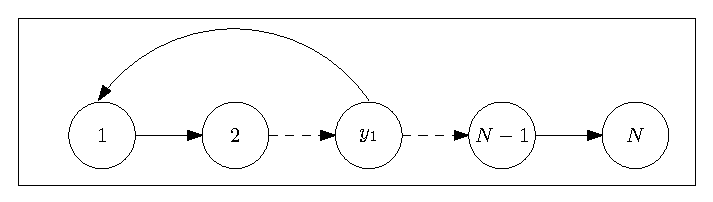
\includegraphics[scale=0.28, keepaspectratio]{Images/WithLeader.eps}\\
			\label{ChainLeader}
			\textnormal{\tiny(a) Directed Cycle With Leader}
		\end{minipage}
		\hspace{1em}
		\begin{minipage}[]{0.44\linewidth}
			\centering
			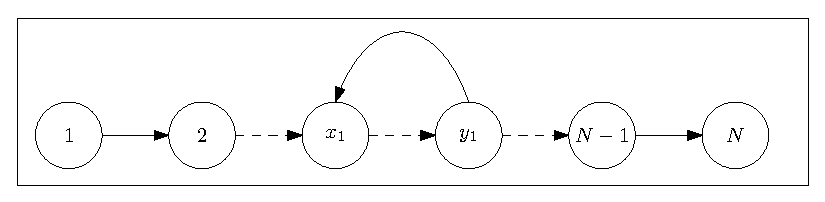
\includegraphics[scale=0.28, keepaspectratio]{Images/WithoutLeader.eps}\\
			\label{ChainWithoutLeader}
			\textnormal{\tiny(b) Directed Cycle Without Leader}
		\end{minipage}
	\end{figure}
	\vspace*{0.1cm}
	%\alt<1-2>{\let\thefootnote\relax\footnotetext{~}}
	{\footnotetext[1]{\textcolor{blue}{Ren W, Atkins E}, {\em Second-order consensus protocols in multiple vehicle systems with local interactions}, AIAA guidance, navigation, and control conference and exhibit 2005.}}
	%\alt<1-3>{\let\thefootnote\relax\footnotetext{~}}
	{\footnotetext[2]{\textcolor{blue}{Yu, Wenwu and Chen, Guanrong and Cao, Ming}, {\em Some necessary and sufficient conditions for second-order consensus in multi-agent dynamical systems}, Automatica 2010.}}		
	%\vspace{-0.5cm}	
\end{frame}


\begin{comment}
\begin{frame}{Problem 1}
	%\vspace{-0.2cm}
	\begin{block}{Problem Statement}
		Consider a \textcolor{blue}{directed chain/path of double integrators containing one leader} node following the consensus protocol \eqref{eq:agent-wise}. Suppose a reverse edge is added to this network to result in a \textcolor{blue}{directed cycle} that may or may not include the leader (as shown below).
	\end{block}
	\begin{figure}
		\centering
		\begin{minipage}[]{0.44\linewidth}
			\centering
			\includegraphics[height=1.2cm, keepaspectratio]{WithLeader.eps}\\
			\label{ChainLeader}
			\textnormal{(a) Directed Cycle With Leader}
		\end{minipage}
		\hspace{1em}
		\begin{minipage}[]{0.44\linewidth}
			\centering
			\includegraphics[height=1.2cm, keepaspectratio]{WithoutLeader.eps}\\
			\label{ChainWithoutLeader}
			\textnormal{(b) Directed Cycle Without Leader}
		\end{minipage}
	\end{figure} 
	\textcolor{blue}{The Objective: }Design suitable \emph{local} strategy/strategies to ensure that consensus does not break down, without adjusting any global variable such as $\gamma$.\\
	\begin{block}{Decentralized solution}
		By \emph{local} strategies, it is implied that the nodes forming the cycle should not be required to possess information about the complete Laplacian spectra.
	\end{block}
\end{frame}

\end{comment}


\begin{subframe}{Laplacian Structure}\label{LapStruct}
	%\vspace{-1cm}
	\textbf{Network Under consideration}:  -- A chain/directed path with $N$ nodes adhering to topological ordering,\\  --A single reverse edge from node $y_1$ to node $x_1$ ($y_1>x_1$) so that the length of the directed cycle is $\ell=y_1-x_1$.\\
	\textbf{Consequence}: Under topological ordering, the Laplacian will have a lower triangular structure:
	%\begin{figure}
		%\centering
		\begin{columns}
			\begin{column}{0.28\textwidth}
			~~	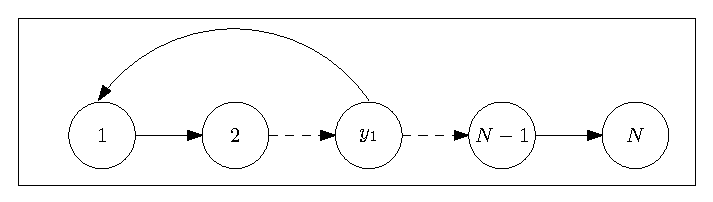
\includegraphics[scale=0.3, keepaspectratio]{Images/WithLeader.eps}
			\end{column}
			\hspace*{-0.5cm}
			\begin{column}{0.22\textwidth}
				$\mathcal{L}=\begin{bmatrix}
					\mathcal{C} & & 0 \\
					& & \\
					* & & \mathcal{L}_2
				\end{bmatrix}$,
			\end{column}
			
			%\centering
			%\label{ChainLeader}
			%\textnormal{(a) Directed Cycle With Leader}
		%\end{minipage}
	%	\hspace{0.5em}
		\begin{column}{0.28\textwidth}
			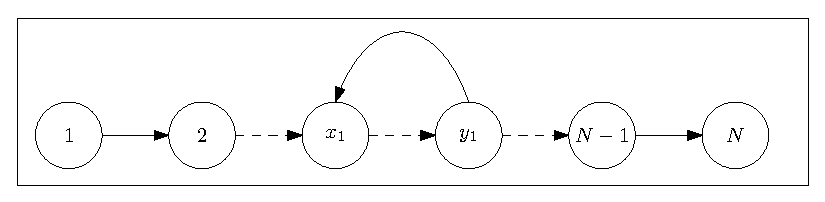
\includegraphics[scale=0.3, keepaspectratio]{Images/WithoutLeader.eps}
		\end{column}
		\begin{column}{0.22\textwidth}
			$\mathcal{L}=\begin{bmatrix}
				\mathcal{L}_1 & 0 & 0 \\
				* & \mathcal{C} & 0 \\
				* & * & \mathcal{L}_2
			\end{bmatrix}$
		\end{column}
		\end{columns}
			%\label{ChainWithoutLeader}
			%\textnormal{(b) Directed Cycle Without Leader}
%$		\end{minipage}
%	\end{figure}
	where $\mathcal{L}_2 \in \mathbb{R}^{(N-y_1) \times (N-y_1)}$,~~ $\mathcal{L}_1 \in \mathbb{R}^{(x_1-1) \times (x_1-1)}$ and $\mathcal{C} \in \mathbb{R}^{(\ell+1) \times (\ell+1)}$.\\
	\vspace{0.2cm}
	\textbf{Case 1:} \textcolor{blue}{With Leader}, $x_1=1 \implies \mathcal{L}_1$ vanishes and $\mathcal{C} \in \mathbb{R}^{y_1 \times y_1}$ exists.\\
	\textbf{Case 2:} \textcolor{blue}{On second reverse edge addition, Laplacian structure remains the same}.\\
	%\centering
	$$\mathcal{L}_2 \in \mathbb{R}^{(N-z_2) \times (N-z_2)},~~\mathcal{L}_1 \in \mathbb{R}^{(z_1-1) \times (z_1-1)},~~\mathcal{C} \in \mathbb{R}^{(z_2-z_1+1) \times (z_2-z_1+1)}$$\\ where $z_1=\min(x_1,x_2),z_2=\max(y_1,y_2)$.\\
	\textbf{Case 3:} Any change in the \textcolor{blue}{$\gamma$ bound is reflected by change in spectra of matrix $\mathcal{C}$}. 
	\hyperlink{BetterSuff}{\beamerbutton{Back}}
\end{subframe}

%\section{\color{blue} Effect of Second Reverse Edge on the Consensus of Double Integrators}
%%%%%%%%%%%%%%%%%%%%%%%%%%%%%%%%%%%%%%%%%%%%%%%%%%%%%
%\begin{frame}[noframenumbering]
%	\tableofcontents[currentsection]
%\end{frame}
%%%%%%%%%%%%%%%%%%%%%%%%%%%%%%%%%%%%%%%%%%%%%%%%%%%%
\begin{frame}
	%\centering
	\textcolor{blue}{Approach 1:} Can we add another cycle in the network to reduce or remove this bound?\\ 
	%\pause
	\vspace{-0.2cm}
	%There are 6 different cases of the second cycle interaction in the said network topology. 
	%Let $\mathcal{V}_1,\mathcal{E}_1$ be the node and edge set of first cycle and $\mathcal{V}_2,\mathcal{E}_2$ be the node and edge set of the second cycle. \vspace{-0.5cm} %Let the characteristic equation be represented by polynomial $p(s)$, where $s=1-\lambda$ and $\lambda$ are the eigenvalues of the matrix $\mathcal{C}$\\
	\begin{figure}
		\centering
		\subfloat[]%t[$\mathcal{V}_1 \cap \mathcal{V}_2=\phi,\mathcal{E}_1 \cap \mathcal{E}_2=\phi$]
		{
			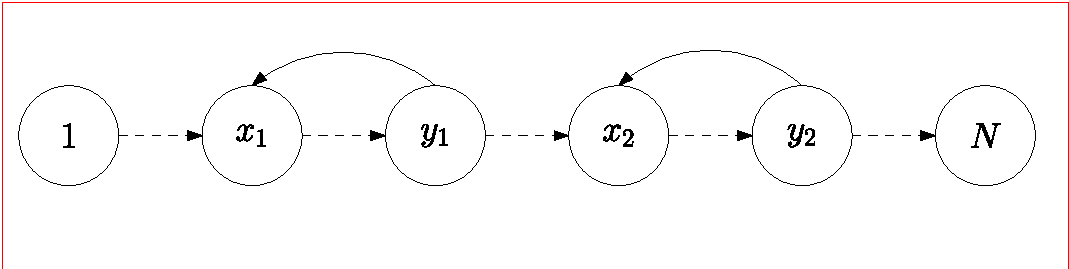
\includegraphics[width=0.35\textwidth,keepaspectratio]{Images/Fig1.pdf}
		}
		\subfloat[]%[$\mathcal{V}_1 \cap \mathcal{V}_2\neq \phi,\mathcal{E}_1 \cap \mathcal{E}_2=\phi$]
		{
			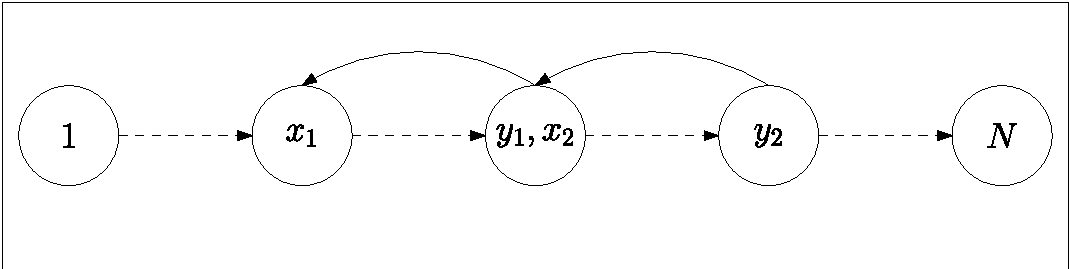
\includegraphics[width=0.35\textwidth,keepaspectratio]{Images/Fig2.pdf}
		}
		\vspace{-3mm}
		\subfloat[]%[$\mathcal{V}_2 \not\subset \mathcal{V}_1,\mathcal{E}_1 \cap \mathcal{E}_2 \neq \phi$]
		{
			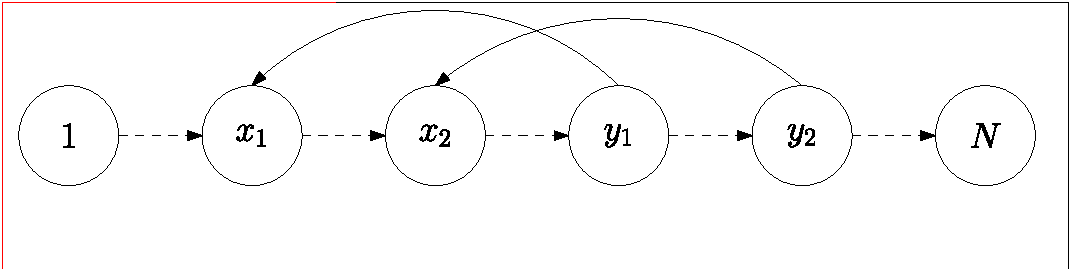
\includegraphics[width=0.35\textwidth,keepaspectratio]{Images/Fig3.pdf}
		}
		\subfloat[]%[$\mathcal{V}_2 \subset \mathcal{V}_1,\mathcal{E}_1 \cap \mathcal{E}_2 \neq \phi,y_2 \neq y_1,x_2 \neq x_1$]
		{
			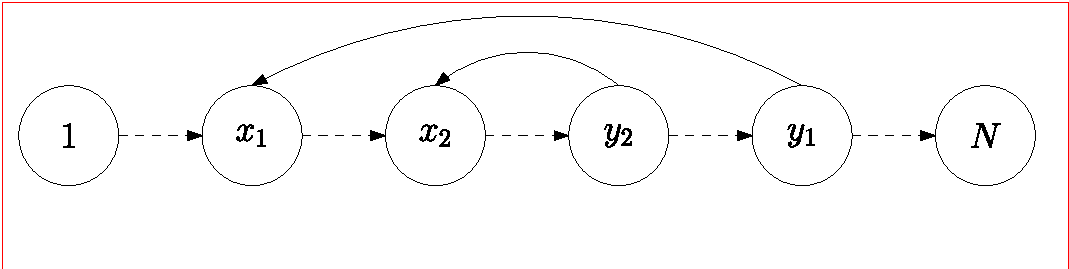
\includegraphics[width=0.35\textwidth,keepaspectratio]{Images/Fig4.pdf}
		}
		\vspace{-3mm}
		\subfloat[]%[$\mathcal{V}_2 \subset \mathcal{V}_1,\mathcal{E}_1 \cap \mathcal{E}_2 \neq \phi,y_2=y_1,x_2 \neq x_1$]
		{
			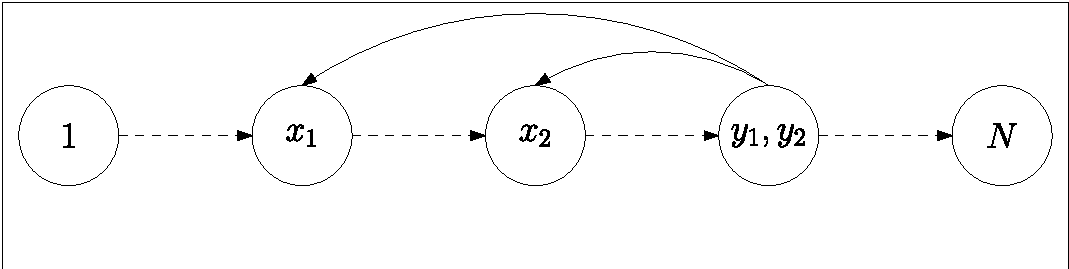
\includegraphics[width=0.35\textwidth,keepaspectratio]{Images/Fig5.pdf}
		}
		\subfloat[]%[$\mathcal{V}_2 \subset \mathcal{V}_1,\mathcal{E}_1 \cap \mathcal{E}_2 \neq \phi,y_2 \neq y_1,x_2=x_1$]
		{
			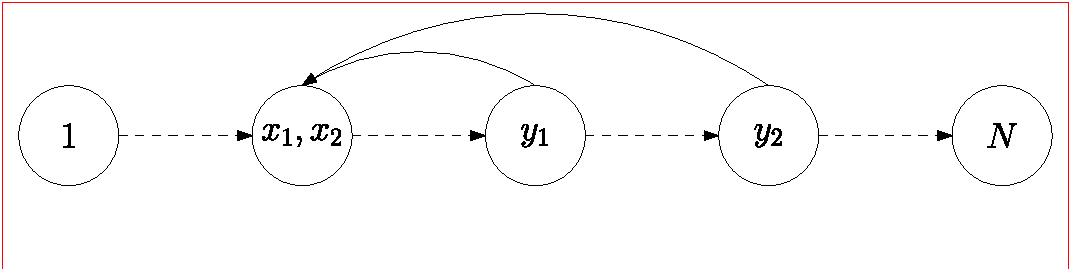
\includegraphics[width=0.35\textwidth,keepaspectratio]{Images/Fig6.pdf}
		}
		\vspace{-2mm}
		%\caption{Different Case of Two reverse Edge Interactions in a chain network}
	\end{figure}
	%\vspace{-0.5cm}
	%\pause
	\textbf{Note 1:} Red boxes indicates similar work by other researchers but in context to single integrators\footnotemark[1]$^,$\footnotemark[2]
	\vspace{0.1cm}
	\footnotetext[1]{\textcolor{blue}{Hao Y, Wang Q, Duan Z,Chen G}, {\em The role of reverse edges on consensus performance of chain networks}, IEEE Transactions on Systems, Man, and Cybernetics: Systems 2019.}
	\footnotetext[2]{\textcolor{blue}{H. -T. Zhang, Z. Chen and X. Mo}, {\em Effect of Adding Edges to Consensus Networks With Directed Acyclic Graphs}, IEEE Transactions on Automatic Control, 2017.}.\\
%	\textbf{Note 2:} Fig. (a)-(c) can be further divided in three sub-cases (i)$l_1>l_2$,(ii)$l_1<l_2$ and (iii) $l_1 = l_2$.\\
	%\textbf{Note 3:} The claims~\footnotemark[1] would be incorrect if the condition in \textbf{Note 2} is not specified.
	
	%\alt<1>{\let\thefootnote\relax\footnotetext{~}}{\footnotetext[1]{\textcolor{blue}{Hao Y, Wang Q, Duan Z,Chen G}, {\em The role of reverse edges on consensus performance of chain networks}, IEEE Transactions on Systems, Man, and Cybernetics: Systems 2019.}}
	%\alt<1>{\let\thefootnote\relax\footnotetext{~}}{\footnotetext[2]{\textcolor{blue}{H. -T. Zhang, Z. Chen and X. Mo}, {\em Effect of Adding Edges to Consensus Networks With Directed Acyclic Graphs}, IEEE Transactions on Automatic Control, 2017.}}
\end{frame}


\begin{subframe}
	The $\gamma$ bound is characterized by the eigenvalues of matrix $\mathcal{C}$ captured in the Laplacian matrix by the reverse edge addition as:\\
	%\centering
	$$\mathcal{L}=\begin{bmatrix}
		\mathcal{L}_1 & 0 & 0 \\
		* & \mathcal{C} & 0 \\
		* & * & \mathcal{L}_2
	\end{bmatrix} \text{ (without Leader)}$$ 
	\vspace{0.2cm}
	Let the characteristic equation of the matrix $\mathcal{C}$ be represented by the polynomial $$\chi(s)=p(s)-1,$$ where $s=1-\lambda$ and $\lambda$ are the eigenvalues of the matrix $\mathcal{C}$\\
	\vspace{-0.2cm}
	%\pause
	%\begin{block} {Polynomial Equations}
	%Then the polynomial equation p(s) will take either one of the form:
	%\begin{enumerate}
	%	\item %\begin{equation} \label{Polynomial1}
	%$p(s,l_2)=s^{l_2+2}+2s^{l_2+1}+s^{l_2}-2s=1, l_2 \in \mathbb{N} \text{ and }l_2 \geq 1$.
	%\end{equation}
	%with $l_2 \in \mathbb{N}$ and $l_2 \geq 1$.
	%\item %\begin{equation} \label{Polynomial2}
	%	$p(s,l_1,l_2)=s^{l_2+2}+2s^{l_2+1}+s^{l_2}-s^{l_2-l_1+1}-s=1, l_2,l_1 \in \mathbb{N}\text{ and }l_2>l_1 \geq 1.$
	%\end{equation}
	%with $l_2,l_1 \in \mathbb{N}$ and $l_2>l_1 \geq 1$.
	%\item %\begin{equation} \label{Polynomial3}
	%$p(s,l_1,l_2)=s^{l_1}(s+2)-s^{l_1-l_2}=1, l_2,l_1 \in \mathbb{N}\text{ and }l_1>l_2 \geq 1.$
	%\end{equation}
	%with $l_2,l_1 \in \mathbb{N}$ and $l_1>l_2 \geq 1$.
	%\item %\begin{equation} \label{Polynomial4}
	%$p(s,l_1,l_2)=s^{l_1+1}+2s^{l_1}+s^{l_1-1}-s^{l_1-l_2}-s^{l_1-l_2-1}=1, l_2,l_1 \in \mathbb{N}\text{ and }l_1>l_2 \geq 1.$
	%\end{equation}
	%with $l_2,l_1 \in \mathbb{N}$ and $l_1>l_2 \geq 1$.
	%\item %\begin{equation} \label{Polynomial5}
	%$p(s,l_1,l_2)=s^{l_i+1}+s^{l_i}=1, l_i=\max(l_1,l_2).$
	%\end{equation}
	%with $l_i=\max(l_1,l_2)$
	%\end{enumerate}
	%\pause
	The following statements are always true for equation p(s):
	\begin{enumerate}
		\item It has only one real solution between (0,1) say $s_1$.
		\item Real parts of other roots are smaller than $s_1$.
		\item $s_1$ is a strictly increasing function of $l_2$.
	\end{enumerate}
	\hyperlink{BetterSuff}{\beamerbutton{Back}}~~\hyperlink{Conc:Approach1}{\beamerbutton{Approach1}}
\end{subframe}


%\pause
\begin{comment}
	\begin{block}{Theorem 1}
		Consensus among double integrators, described by \eqref{SecondConsensus}, is achieved asymptotically if the networked system has a directed spanning tree and \\
		\begin{equation}\label{new-sufficiency}
			\gamma \geq \frac{1}{\sqrt{1-s_1}}=\frac{1}{\sqrt{\lambda_1}} \text{  \bigg(Better Sufficient Condition, \textcolor{red}{Earlier $\frac{2}{\sqrt{\lambda_1}}$}\bigg)}
		\end{equation}	
		where $s_1$ is the real solution of the relevant polynomial equations p(s) and $\lambda_1$ is the corresponding eigenvalue of the matrix $\mathcal{C}$ based on lengths of directed cycle and the interaction among the two cycles.
	\end{block}	
\end{comment}
%\end{block}


\begin{subframe}
	\vspace{-0.1cm}
	\begin{theorem}[Better Sufficiency Condition]\label{BetterSuff}
		Consensus among double integrators is achieved asymptotically if the networked system has a directed spanning tree and \\
		\begin{equation*}\label{new-sufficiency}
			\gamma \geq \frac{1}{\sqrt{1-s_1}}=\frac{1}{\sqrt{\lambda_1}} \text{  \bigg(Better Sufficient Condition, \textcolor{red}{Earlier $\frac{2}{\sqrt{\lambda_1}}$}\bigg)}
		\end{equation*}	
		where $s_1$ is the real solution of the relevant polynomial equations p(s) and $\lambda_1$ is the corresponding eigenvalue of the matrix $\mathcal{C}$. %based on lengths of directed cycle and the interaction among the two cycles. 
		\hyperlink{LapStruct}{\beamerbutton{$\mathcal{C} Structure$}}
	\end{theorem}	
	\vspace{-0.2cm}
	\begin{theorem}[Effect of Cycle on Eigenvalues]
		A cycle of length $l$ on a directed chain of $N$ nodes affects $l$ eigenvalues of the Laplacian if such a cycle contains the root node, and affects $l+1$ eigenvalues otherwise.
	\end{theorem}
	\vspace{-0.2cm}
	\begin{block}{Conclusions}
		\begin{enumerate}
			\item Deduced better sufficiency condition
			\item Need not to search over the entire spectra but the knowledge of the only real root is sufficient.
			\item The lengths of cycle and their relative positions are sufficient for finding the bound and is independent of the network size. \hyperlink{Conc:Approach1}{\beamerbutton{Approach1}}
		\end{enumerate}
	\end{block}
	
\end{subframe}

%\section{\color{blue}Guaranteeing Consensus of Double Integrators in Presence of a Directed Cycle}\label{Conc:Approach1}
\begin{frame}
	\begin{block}{Results from approach 1}
		\begin{enumerate}
			\item We were able to achieve better sufficiency condition than the one in the literature.\hyperlink{BetterSuff}{\beamerbutton{Theorem}}
			\item We proposed a polynomial-based approach where the roots are determined by the cycle in the loop, and the real root alone is sufficient to compute the sufficiency condition.
			\item The lengths of cycle and their relative positions are sufficient for finding the bound and is independent of the network size. 
		\end{enumerate}
	\end{block}
	\begin{block}{Challenges in Approach 1:}
		\begin{enumerate}
			\item The polynomial-based approach fails to analyze scenarios where the leader is part of the directed cycle.
			\item It simplifies computation but does not help in reducing or eliminating the bound.
			\item Not a local remedy as requires every agent to update the $\gamma$ value to achieve consensus.
		\end{enumerate}
	\end{block}
	\textcolor{blue}{Publications: }\\
	\begin{enumerate}
		\item Dubey, A. K., Mukherjee, D., \& Arya, K. (2022). Consensus of double integrators over a chain with reverse edges. IFAC-PapersOnLine, 55(13), 19-24.
	\end{enumerate}
	%\pause
	%\centering So can't we reduce the bound? \pause~~~\textcolor{blue}{Yes, We can}\\
	\vspace{0.2cm}
\end{frame}

\begin{frame}{Approach 2: Edge Weight Perturbation}\label{gersback}
	%\textcolor{blue}{Methodology} Using edge weight perturbation of the cycles and/or neighboring edge to the cycle, to 
	\textcolor{brown}{Guaranteed the consensus} for any pre-designed velocity coupling factor.\\ %Not only \textcolor{cyan}{for the leaderless case} but also for the case where \textcolor{cyan}{the directed cycle involves leader}.
	%\begin{itemize}
		%\item 
		-- \textcolor{blue}{Directed cycle without leader} $\rightarrow$ Guaranteed the consensus using the Node Scaling, the Edge Scaling and the combined scaling methods utilizing the Gershgorin's disc theorem. 
				\begin{columns}
					\begin{column}{0.5\textwidth}
						\begin{figure}
							\centering
							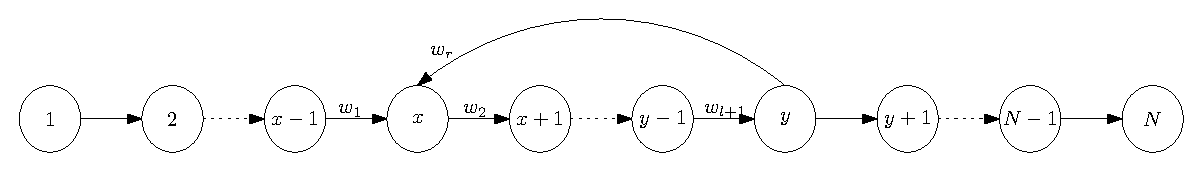
\includegraphics[scale=0.35,keepaspectratio]{Images/EdgeScaling.eps}
							\caption{Edge Scaling Method}
							%\label{EdgeScaledNetwork}
						\end{figure}
					\end{column}
					\begin{column}{0.5\textwidth}
						\begin{figure}
							\centering
							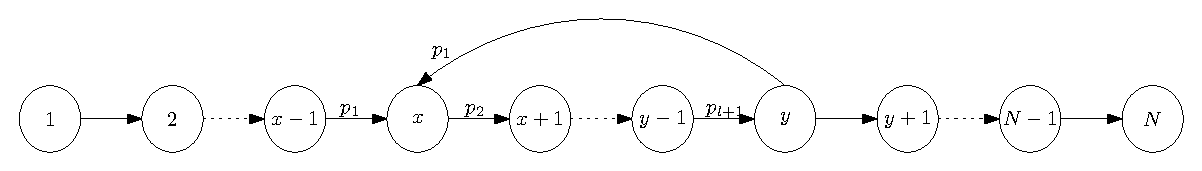
\includegraphics[scale=0.35,keepaspectratio]{Images/NodeScaling.eps}
							\caption{Node Scaling method}
							%\label{EdgeScaledNetwork}
						\end{figure}
					\end{column}
				\end{columns}
		%\item For directed cycle with leader $\rightarrow$ Root Locus Based approach.
	%\end{itemize}
	\hyperlink{NSSimbase}{\beamerbutton{{NS Method}}}~~\hyperlink{ESSimbase}{\beamerbutton{{ES Method}}}~~\hyperlink{CombScal}{\beamerbutton{{NES Method}}}~~ \hyperlink{gers}{\beamerbutton{Gershgorin's Theorem}}\\
	\pause
	-- \textcolor{blue}{Directed cycle with leader}
	\begin{itemize}
		\item Guranteed the consensus for a situation that has not been analyzed enough in the literature.
		\item Utilized a simple root locus based strategy, again applicable locally, to mitigate the adverse effects of the reverse edge.\hyperlink{RLSimbase}{\beamerbutton{RLS Method}}
		\item Contrary to the node scaling and the edge scaling methods, where increasing the scaling parameters assists in consensus, here one of the gain $\beta$ needs to be bounded above, while the other gain $\alpha$ is to be chosen large for achieving the consensus.
	\end{itemize}
	%\begin{block}{Future Work}
	%	\begin{itemize}
	%		\item To obtain a tighter lower bound on the coupling factor $\gamma$ by using both the real and imaginary parts of the eigenvalues.
	%		\item Considering more general types of directed acyclic graphs also remains an important problem to be addressed within this set-up.
	%	\end{itemize}
	%\end{block}
\end{frame}
%%%%%%%%%%%%%%%%%%%%%%%%%%%%%%%%%%%%%%%%%%%%%%%%%%%%%%%%%%%%%%%%%%%%%%%%%%%%%%%%%%
\begin{frame}
	\begin{block}{Conclusion}
		\begin{itemize}
			\item Guaranteed consensus for any pre-designed value of $\gamma$ .
			\item Can be applied locally and the agents outside the directed cycle need not alter their control laws.
			\item Adressed the case when the leader in the chain is forced into a directed cycle, a situation that has not been analyzed enough in the literature.
		\end{itemize}
	\end{block}
	\textcolor{blue}{Publications: }\\
	\begin{enumerate}
		\item Dubey, A. K., Mukherjee, D., \& Arya, K. (2023, May). Consensus of double integrators in presence of a reverse edge in a chain: Analysis and design. In 2023 American Control Conference (ACC) (pp. 411-416). IEEE.
		\item Dubey, A. K. \& Mukherjee, D.(2024). Guaranteed Consensus in System of Double Integrators in Presence of Directed Cycles [Journal to be communicated]
	\end{enumerate}
\end{frame}

\begin{subframe}{}
	Why Gershgorin's Theorem work??\\ 
	\pause
	The $\gamma$ bound is characterized by the eigenvalues of matrix $\mathcal{C}$ as:
	$$\mathcal{L}=\begin{bmatrix}
		\mathcal{L}_1 & 0 & 0 \\
		* & \mathcal{C} & 0 \\
		* & * & \mathcal{L}_2
	\end{bmatrix}\text{ (without Leader)}$$
	\vspace{-0.1cm}
	\begin{block}{New Sufficiency Condition}
		$$\gamma \geq \frac{1}{\sqrt{\lambda_1}}$$
		- $\lambda_1$ is the one and only real eigenvalue\\ 
		- $\lambda_1$ is the lowest real eigenvalue
	\end{block}
	\vspace{-0.1cm}
	\begin{exampleblock}{}
		- Zero eigenvalue is part of $\mathcal{L}_1$\\
		- Eigenvalue of $\mathcal{C}$ is all positive.
	\end{exampleblock}
	\vspace{-0.1cm}
	\begin{alertblock}{}
		- Row Picture of Gershgorin's Discs always touches zero\\
		- However, Column Picture of Gershgorin's Discs may not
	\end{alertblock}
	%\textbf{Note 1:} Although the Gershgorin's Discs always touches zero when looking at the row picture but we can ensure that the Gershgorin's discs do not touch zero while looking at the column picture. 
	\hyperlink{Conc:Approach1}{\beamerbutton{Approach1}}
\end{subframe}


\begin{subframe}{Node Scaled Method}\label{NSSimbase}	
	\begin{figure}
		\centering
		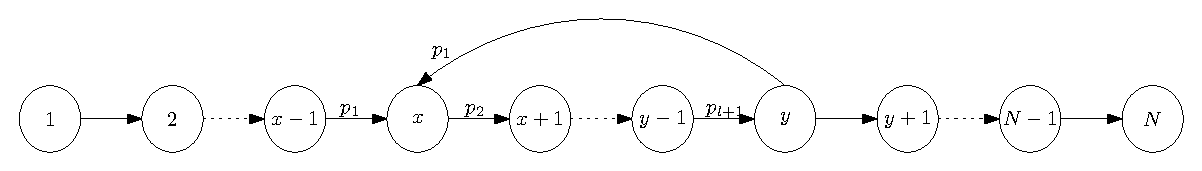
\includegraphics[scale=0.35,keepaspectratio]{Images/NodeScaling.eps}\\
		%\caption{Node Scaled Network}
		%\label{NodeScaledNetwork}
	\end{figure}
	%\pause
	$\Tilde{P}=P\mathcal{C}=\tiny{\begin{bsmallmatrix}
		2p_1  & 0  & \dots & -p_1 \\
		-p_2 & p_2 & \dots & 0 \\
		\vdots & \vdots & \ddots & \vdots \\
		\vdots & \dots & -p_{(\ell+1)} & p_{(\ell+1)}
	\end{bsmallmatrix}},$
	where, $P=\text{diag}(p_1,p_2,p_3,\dots,p_{\ell+1})$ is a matrix with positive entries.
	\vspace{-0.2cm}
	\begin{block}{Objective}
		Applying Gershgorin's Disc theorem to columns 
		$$2p_1>p_2>p_3>\dots>p_{\ell+1}>p_1$$
		
		- Ensure it is separated from origin \\
		- Maximize the distance of closest disc\\
		\textcolor{blue}{Solution: }Create an Arithmetic Progression between the elements of inequality above.
	\end{block}
	Consensus is achieved if:		$p_{i-x_1+1}=\frac{\ell+1}{\gamma^2}+\epsilon+(i-x_1)\frac{[(\ell+1)/\gamma^2]+\epsilon}{\ell+1}, \epsilon>0.$ \hyperlink{NSSim}{\beamerbutton{Simulations}}~~\hyperlink{gersback}{\beamerbutton{Back2Approach2}}
\end{subframe}



\begin{subframe}{Edge Scaled Method}\label{ESSimbase}
	%\begin{minipage}{0.45\textwidth}
	\begin{figure}
		\centering
		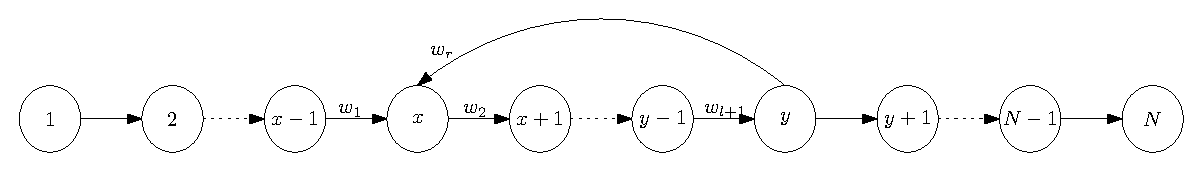
\includegraphics[scale=0.35,keepaspectratio]{Images/EdgeScaling.eps}
		%\caption{Edge Scaled Network}
		\label{EdgeScaledNetwork}
	\end{figure}
	$\Tilde{\mathcal{C}}=\tiny{\begin{bsmallmatrix}
		w_1+w_r  & 0 & \dots & -w_r \\
		-w_2 & w_2 & \dots & 0 \\
		\vdots & \vdots  & \ddots & \vdots \\
		\vdots & \dots & -w_{\ell+1} & w_{\ell+1}
	\end{bsmallmatrix}}$,~~where, $w_i's, i \in \{1,2,\dots,\ell+1\}$ are the forward edge weights and $w_r$ is the forward and reverse edge weight to node $x_1$.\\
	\vspace{-0.2cm}
	\begin{block}{Objective}
		Applying Gershgorin's Disc theorem to columns of $\tilde{\mathcal{C}}$ 
		\vspace*{-0.3cm}
		$$w_1+w_r>w_2>w_3>\dots>w_r$$		
		%\vspace*{-0.15cm}
		- Ensure it is separated from origin \\
		- Maximize the distance of closest disc\\
		\textcolor{blue}{Solution: }Create an Arithmetic Progression between the elements of inequality above.
	\end{block}
	\vspace*{-0.1cm}
	Consensus achieved if:
	$w_1=\frac{\ell+1}{\gamma^2}+\epsilon; w_k=w_1+(k-1)[w_1/(\ell+1)]$, for any $\epsilon>0$ and $k\in\{2,\ldots,\ell+1\}$. \hyperlink{ESSim}{\beamerbutton{Simulations}}~~\hyperlink{gersback}{\beamerbutton{Back2Approach2}}	
	%\end{minipage}
\end{subframe}



\begin{subframe}\label{CombScal}
	\begin{block}{Combined Scaling}
		$$\Tilde{P}=P\Tilde{\mathcal{C}}=\tiny{\begin{bsmallmatrix}
				p_1(w_1+w_f)  &  0 & \dots & -p_1w_1 \\
				-p_2w_2 & p_2w_2 & \dots & 0 \\
				\vdots & \vdots  & \ddots & \vdots \\
				\vdots & \vdots  & -p_{\ell+1}w_{\ell+1} & p_{\ell+1}w_{\ell+1}
		\end{bsmallmatrix}}$$
		where $P$ is the matrix coming from Node Scaling and $\mathcal{C}$ is the matrix coming from Edge Scaling.\\
	\end{block}
	Applying Gershgorin's theorem, we get:\\
	$$p_1(w_1+w_r)>p_2w_2>p_3w_3>\dots>p_1w_r$$
	\textcolor{blue}{Solution: }Create an AP between $p_1(w_1+w_r)$ and $p_1w_r$\\
	\pause
	Why Combine?\\
	\pause
	\textcolor{blue}{Reason:\\ }
	- Greater freedom in parametric choice \\
	- Trade-off between the node and edge scaling parameters.\\
	~~\hyperlink{gersback}{\beamerbutton{Back2Approach2}}
\end{subframe}
	%\pause
	%\hrule
	
	
\begin{subframe}{Directed cycle with root node}
	\textcolor{red}{Will ESS or NSS work for directed cycles with leader ??} \pause \textcolor{blue}{No!! but why ??}\\
	\begin{block}{}
		\begin{itemize}
			\item The edge scaling fails since the edge connecting node $x_1=1$ to $x_1-1$ does not exist (node $0$ is non-existent)
			\item The node scaling method fails because $\Tilde{\mathcal{C}}$ becomes a circulant matrix with a zero eigenvalue, and union of Gershgorin's discs always contains any open neighborhood of the origin.
		\end{itemize}
	\end{block}
	\pause
	\centering
	\textcolor{red}{Solution??} 
	Root Locus Based Methodology ~~\hyperlink{RLSimbase}{\beamerbutton{RLS Method}}
\end{subframe}


\begin{subframe}{Root Locus Method}\label{RLSimbase}
	\vspace*{-0.2cm}
	Choose Node Scaling based approach to scale all but one with scaling factor $\alpha$ and this one node scaling parameter(say for agent $2$) be $\beta$. Then,
	$\Tilde{\mathcal{C}}=\tiny{\begin{bsmallmatrix}
		\alpha  & 0 & \dots & -\alpha \\
		-\beta & \beta & 0 & 0 \\
		\vdots & \vdots & \ddots & \vdots \\
		\vdots & \dots & -\alpha & \alpha
	\end{bsmallmatrix}}$\\
	the $\gamma$ bound as mentioned earlier is driven by the roots of characteristic equation of $\mathcal{C}$ which is given by:\\
	--Characteristic Equation $\chi(s)=1-G(s)=0$, with $G(s)=\frac{\beta\{(s-\alpha)^\ell-(-\alpha)^\ell\}}{s(s-\alpha)^\ell}$.\\
	--Cast as complementary root locus on gain $\beta$.\\
	--Zeros at $\alpha(1-e^{(\iota \frac{\pi}{\ell}(2k))})$ with $k\in\{0,\ldots,\ell-1\}$, where $\iota=\sqrt{-1}$.\\
	\textbf{Note: } The pole at origin is canceled by zero at origin of the G(s).
	\vspace*{-0.2cm}
	\begin{block}{Algorithm}\label{Algo}
		\begin{enumerate}
			\item Choose $\alpha>\frac{1}{\gamma^2}$ and draw the complementary root locus of G(s).
			\item Take it's mirror image by drawing the root locus of G(-s) and shift it by a distance $d=\frac{1}{\gamma^2}$.
			\item Find the gain value at which it remains inside the left half plane.%(\textcolor{red}{It is not equivalent to gain value when it moves to right half})
			\item choose any $\beta$ from that range to guarantee the consensus.
		\end{enumerate}
	\end{block}  
\end{subframe}

%%%%%%%%%%%%%%%%%%%%%%%%%%%%%%%%%%%%%%%%%%%%%%%%%%%%%%%%%%%%%%%%%%%%%%%%%%%%%%%%%%%%%%%
\begin{subframe}{Remarks on Root Locus Approach}
	\begin{enumerate}
		\item Contrary to the node scaling and the edge scaling methods, where increasing the scaling parameters assists in consensus, here the gain $\beta$ needs to be bounded above, while $\alpha$ is to be chosen large.
		\item Note, $\beta=0$ is not a feasible choice, since it implies breaking the cycle that was formed by the reverse edge and is tantamount to dropping an edge altogether, in response to an additional reverse edge.
		\item In most of the literature dealing with consensus in case of perturbed edge weights, such perturbations have mostly been viewed as undesirable, both for undirected and directed graphs. However, we show that a judiciously chosen \emph{perturbation} may also lead to local remedies for a consensus-seeking network of double integrators.
	\end{enumerate} 
	\hyperlink{RLSim}{\beamerbutton{Simulations}}~~\hyperlink{gersback}{\beamerbutton{Back2Approach2}}   
\end{subframe}
%%%%%%%%%%%%%%%%%%%%%%%%%%%%%%%%%%%%%%%%%%%%%%%%%%%%%%%%%%%%%%%%%%%%%%%%%%%%%%%%%%
\begin{comment}
\begin{frame}{Conclusion}
	\begin{block}{Remark on Root locus}
		\begin{itemize}
			\item Need Small $\beta$ unlike node and edge based scaling.
			\item Ideal choice $\beta=0$, \textcolor{red}{Not an appropriate choice}
			\item Edge Perturbation- \textcolor{red}{Bane or Boon?}
		\end{itemize}
	\end{block}
	\begin{block}{Solution to Challenges in Approach 1:}
		\begin{enumerate}
			\item Fails with leader in the directed cycle. \checkmark
			\item Ease computation but not helpful reducing or eliminating the bound. \checkmark
			\item Not a local remedy. \checkmark
			%\paused
		\end{enumerate}
	\end{block}	
	%\pause
	
\end{frame}

\end{comment}



\begin{subframe}{Node Scaling Simulations}\label{NSSim}
	-- Effective length of cycle= $\ell+1=6$ and $\gamma^2=0.16$, Hence, $p_1 \geq \frac{6}{0.16}=37.5$\\
	-- We chose, $p_1=39$, with $diff=39/6=6.5$ and hence, $$P= \text{diag}(39,71.5,65,58.5,52,45.5)$$
	\begin{figure}[ht]
		\centering
		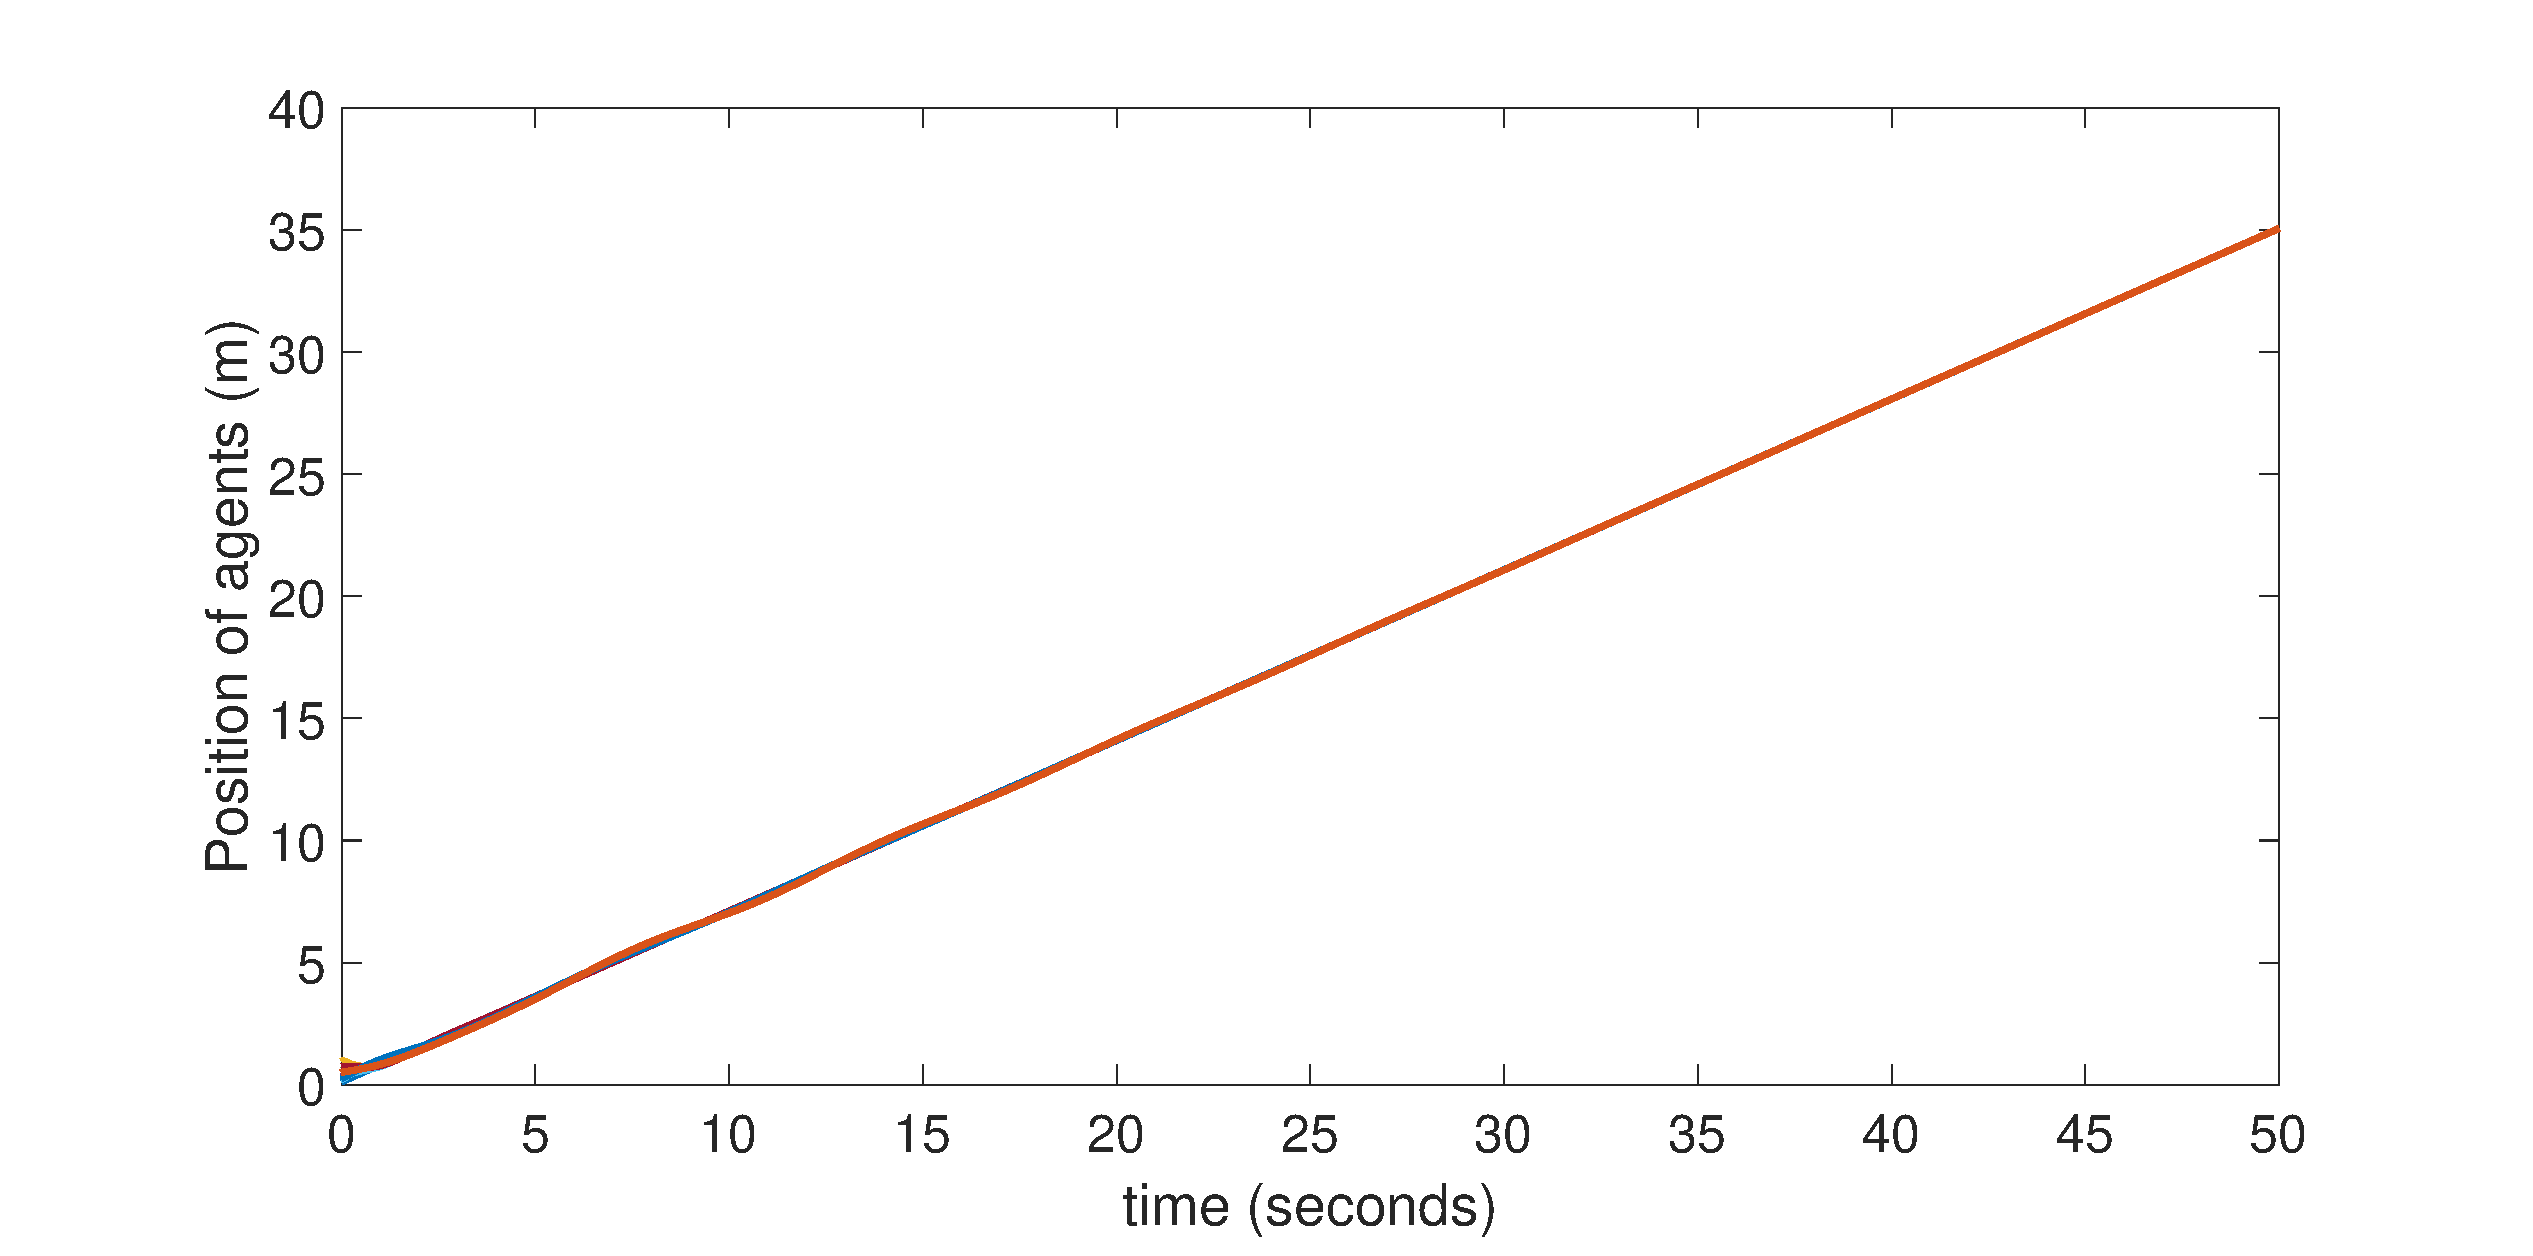
\includegraphics[scale=0.2,keepaspectratio]{Images/9-7-2_NodeScaledlLaplacianGamma0.4PositionConsensus1.eps}
		\caption{Position consensus with node scaled Laplacian for $\gamma = 0.4$}
		\label{NodeScaledLaplacianPositionConsensus0.4}
	\end{figure}
	\vspace{-1.2cm}
	\hyperlink{NSSimbase}{\beamerbutton{Back}}
\end{subframe}


%%%%%%%%%%%%%%%%%%%%%%%%%%%%%%%%%%%%%%%%%%%%%%%%%%%%%%%%%%%%%%%%%%%%%%%%%%%%%%%%%%%%%%%
\begin{subframe}{Edge Scaling Simulations}\label{ESSim}
	--Similar to the node scaling method, here  $w_1 \geq 37.5$ \\
	--We chose, $w_1=39$ and assume $w_r=1$, thus giving $diff=39/6=6.5$ and hence, edge weights $$W= \text{diag}(39,32.5,26,19.5,13,6.5)$$
	\begin{figure}[ht]
		\centering
		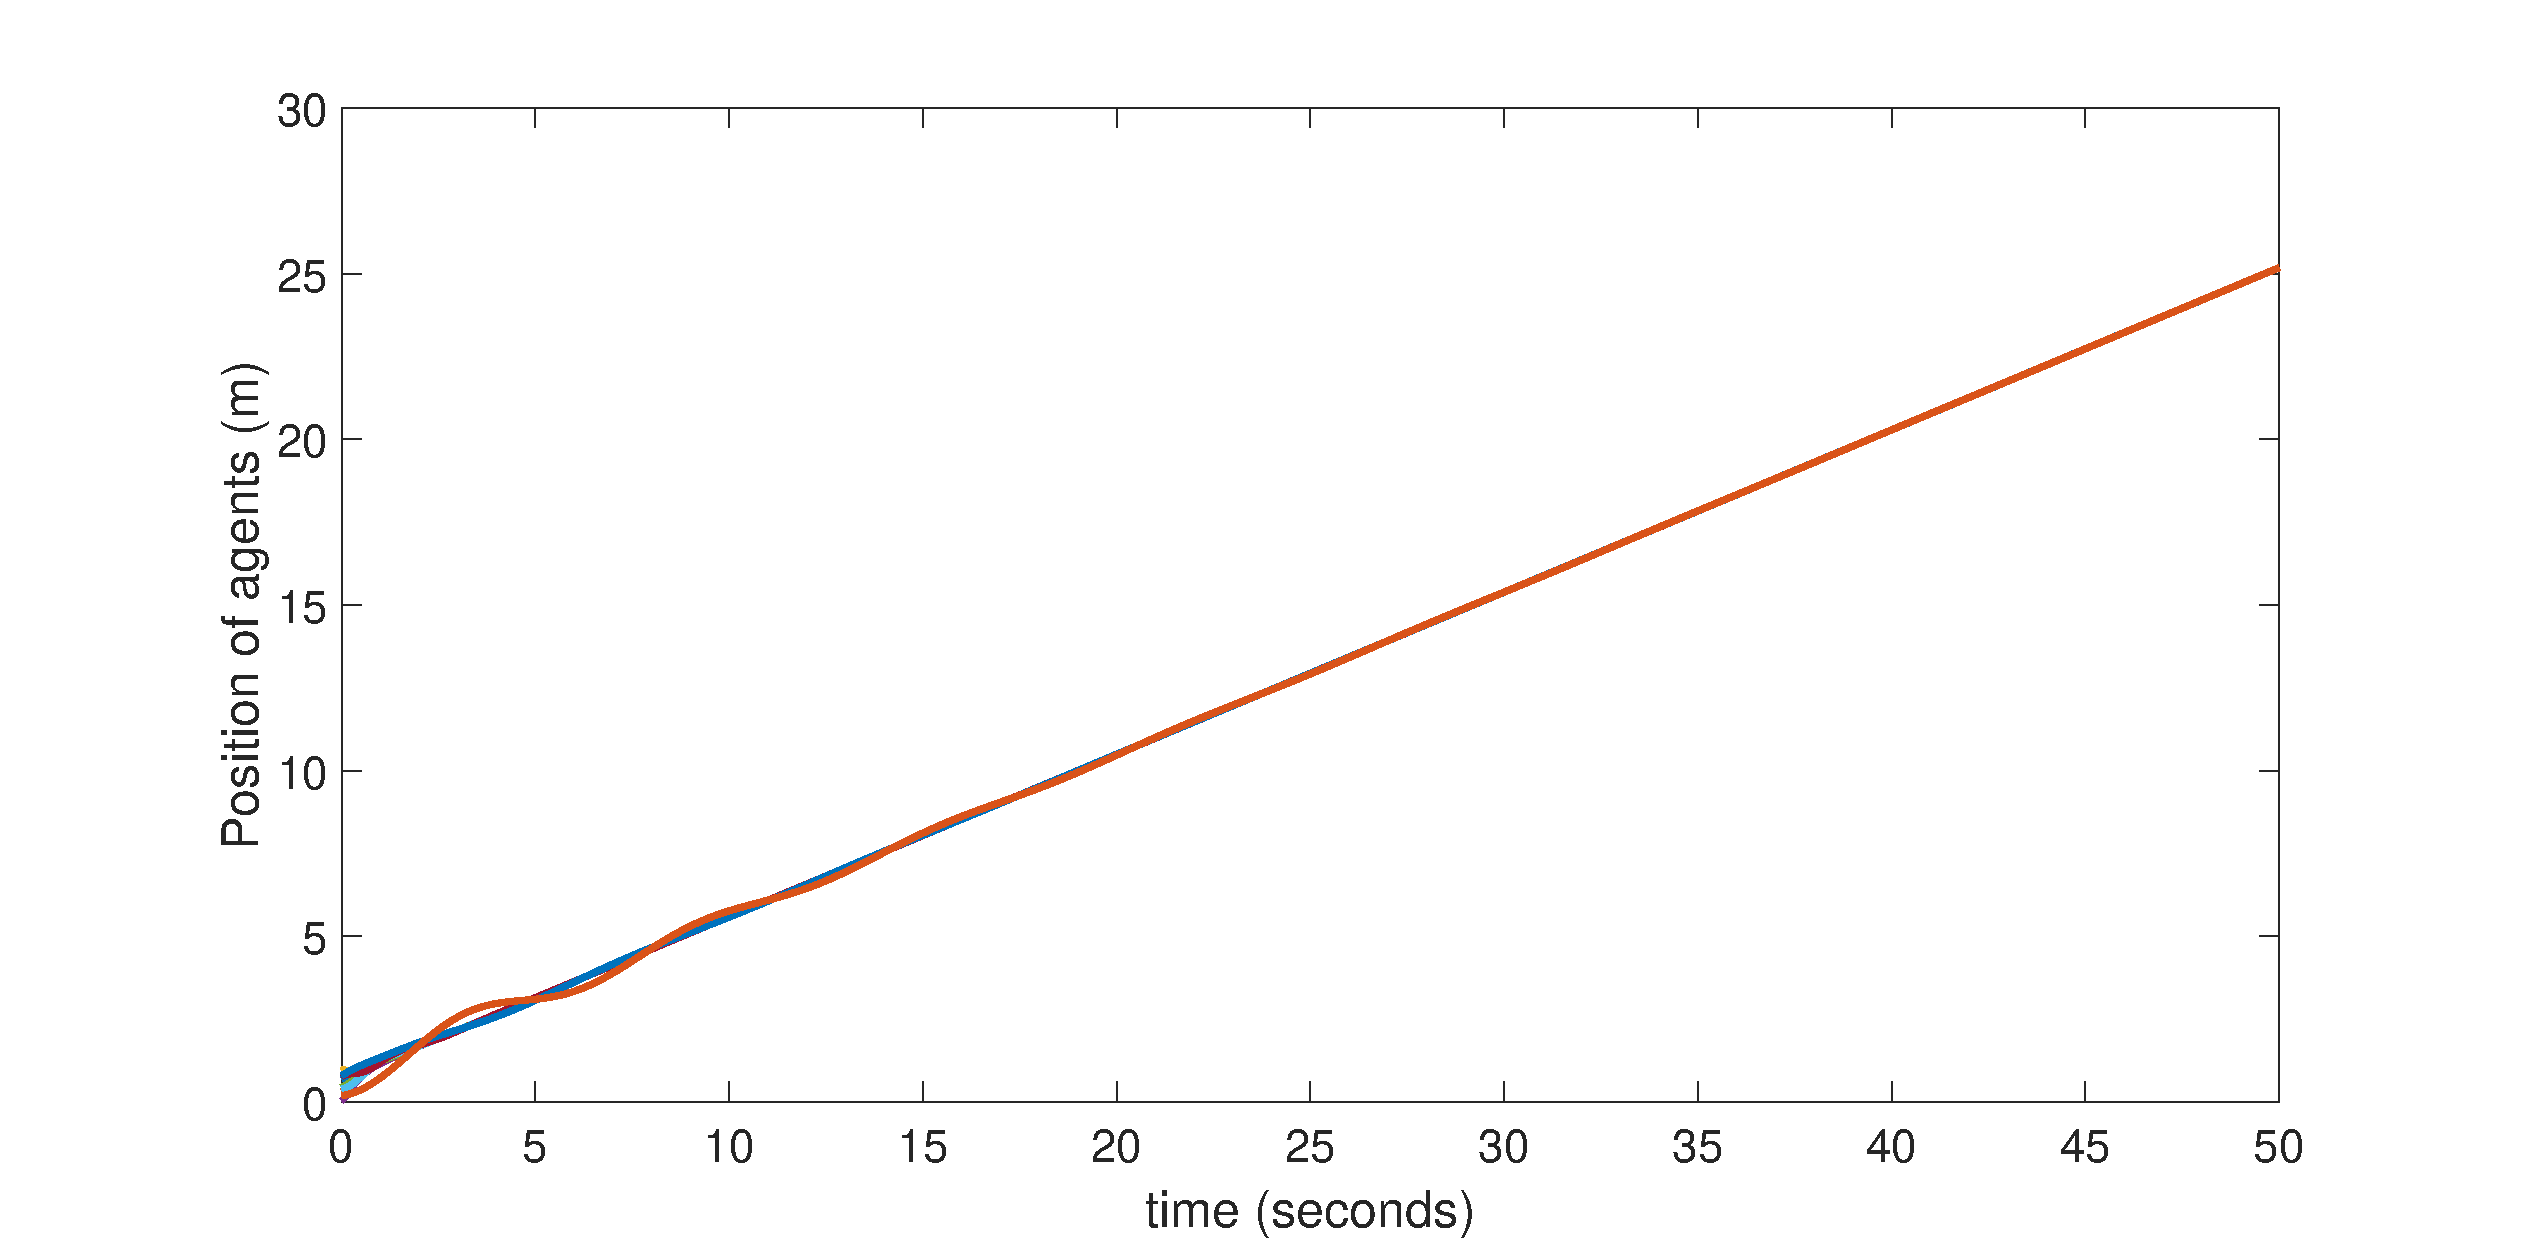
\includegraphics[width=0.5\textwidth,keepaspectratio]{Images/9-7-2_EdgeWeightedlLaplacianGamma0.4PositionConsensus1.eps}
		\caption{Position consensus of edge weight scaled Laplacian with $\gamma = 0.4$}
		\label{EdgeWeightedLaplacianPositionConsensus0.4}
	\end{figure}
	\vspace{-0.3cm}
	\hyperlink{ESSimbase}{\beamerbutton{Back}}
	%\textbf{Note:} Simulation for Combined Method is omitted as it is trivial to achieve consensus but only provides with more flexibility in choosing the design parameters. 
\end{subframe}
%%%%%%%%%%%%%%%%%%%%%%%%%%%%%%%%%%%%%%%%%%%%%%%%%%%%%%%%%%%%%%%%%%%%%%%%%%%%%%%%%%%%%%%


\begin{subframe}{Root Locus Based Simulations}\label{RLSim}	
	We chose $\alpha=10$ and $\tau=9$, and thus from the root locus, we get, $\beta \leq 0.00009$, Thus, we chose $\beta=0.00008$
	\vspace{-0.3cm}	
	\begin{columns}
		\begin{column}{0.5\textwidth}
			\begin{figure}[ht]
				\centering
				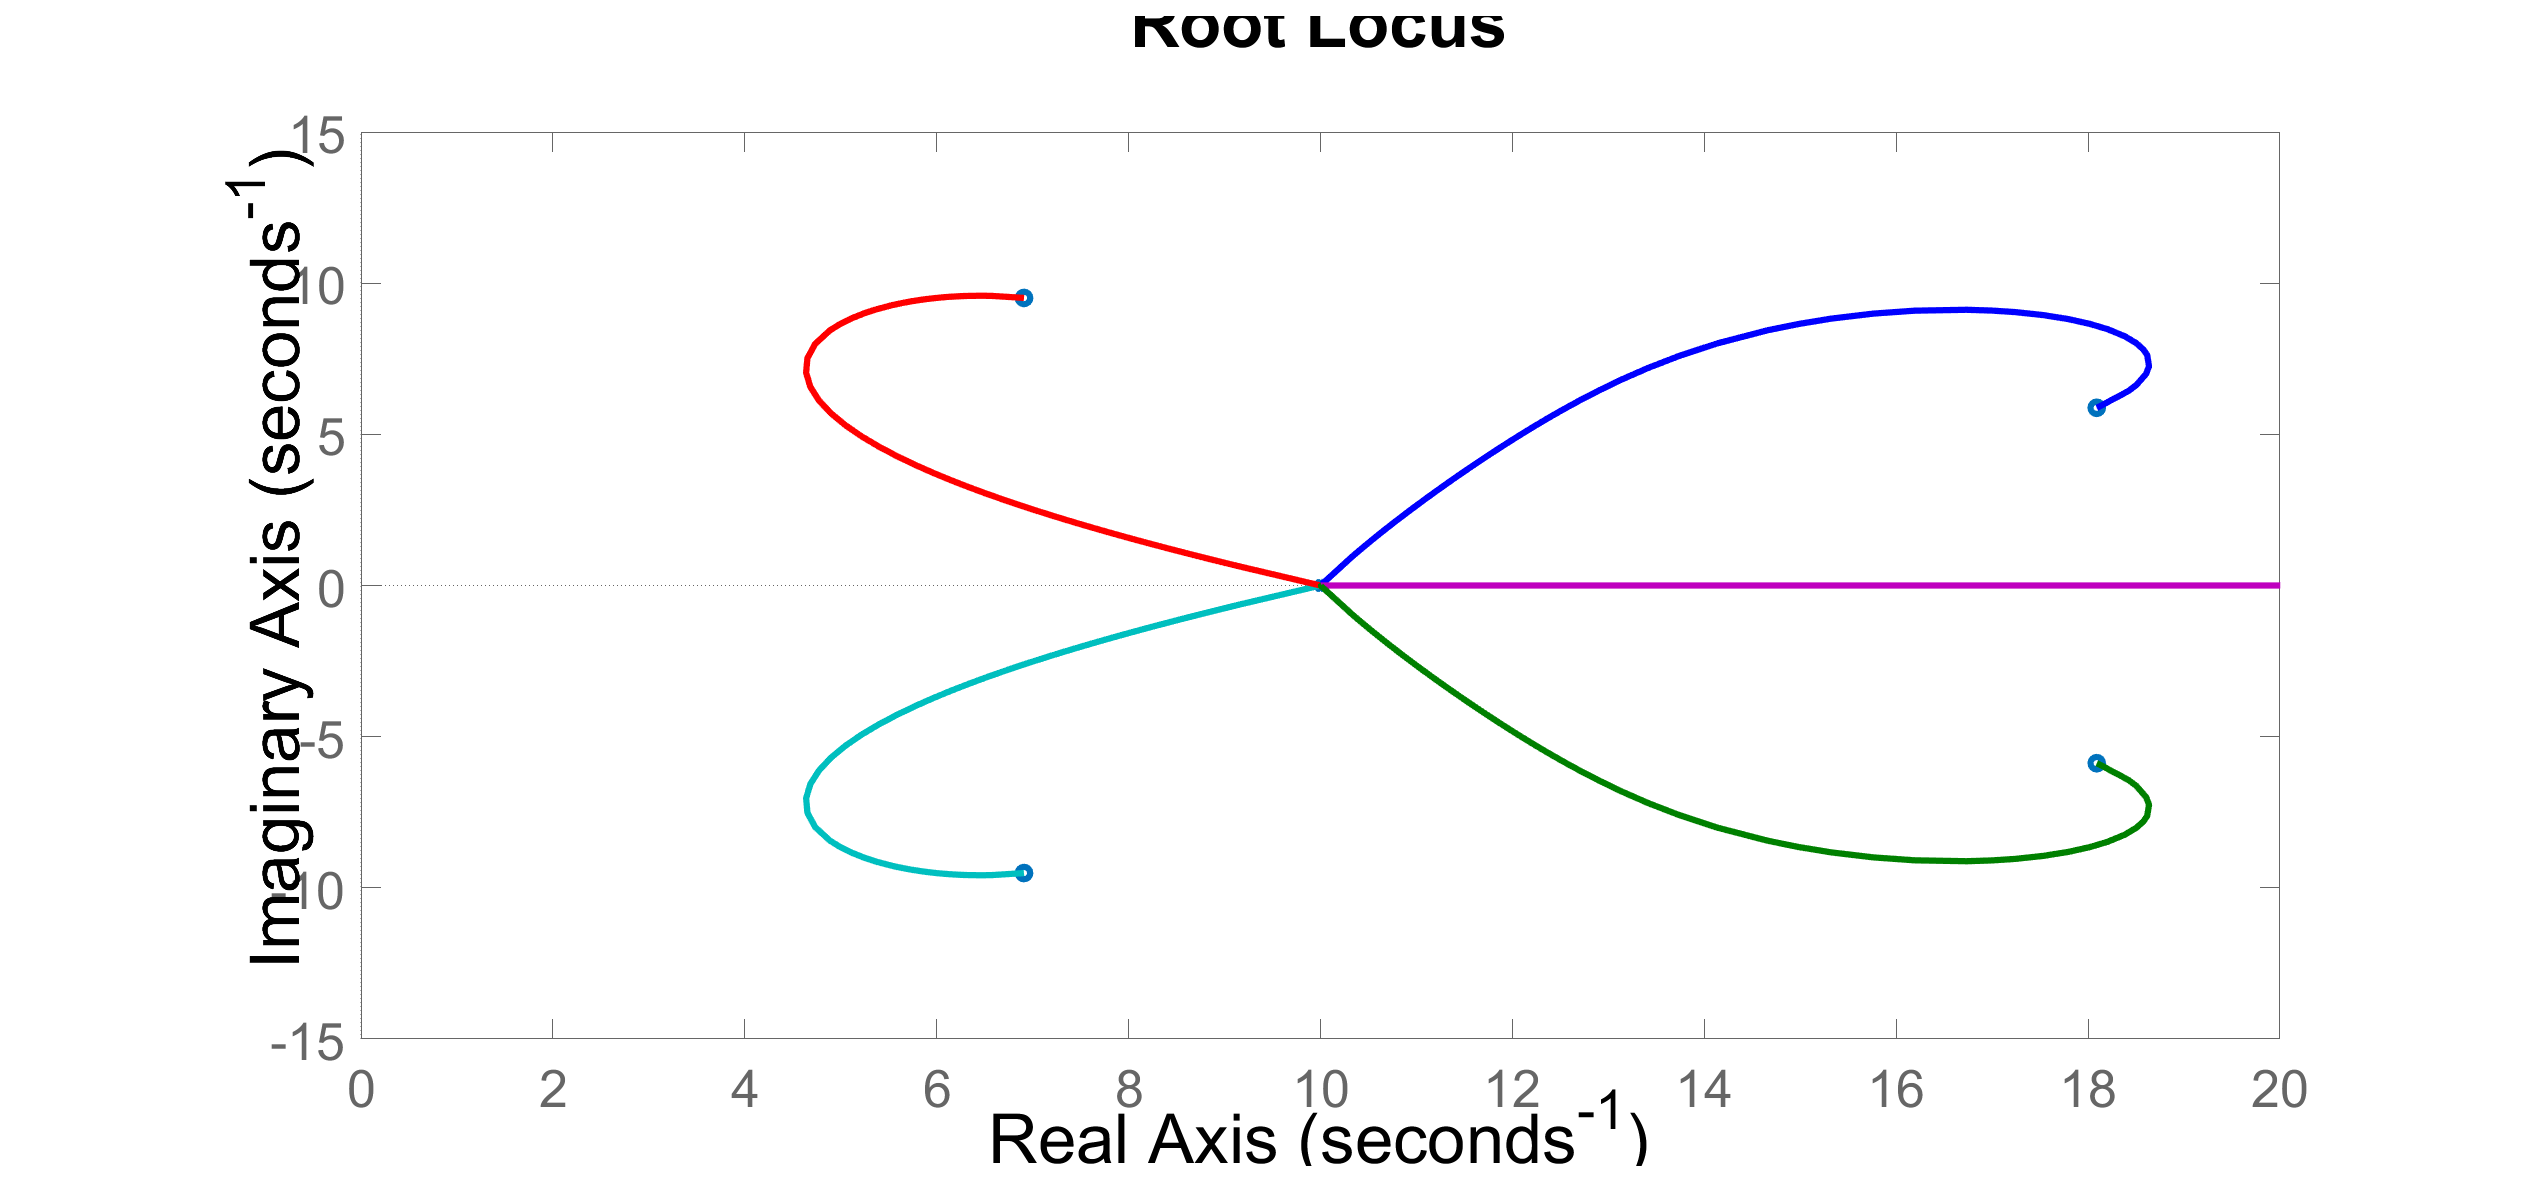
\includegraphics[trim={0 0 0 .6cm},clip,scale=0.18,keepaspectratio]{Images/9-6-1_RootLocus1.eps}
				\caption{Complementary root locus of $G(s)$ when the cycle involves leader}
				\label{ComplimentaryRootLocus}
			\end{figure}
		\end{column}
		\begin{column}{0.5\textwidth}
			\begin{figure}[ht]
				\centering
				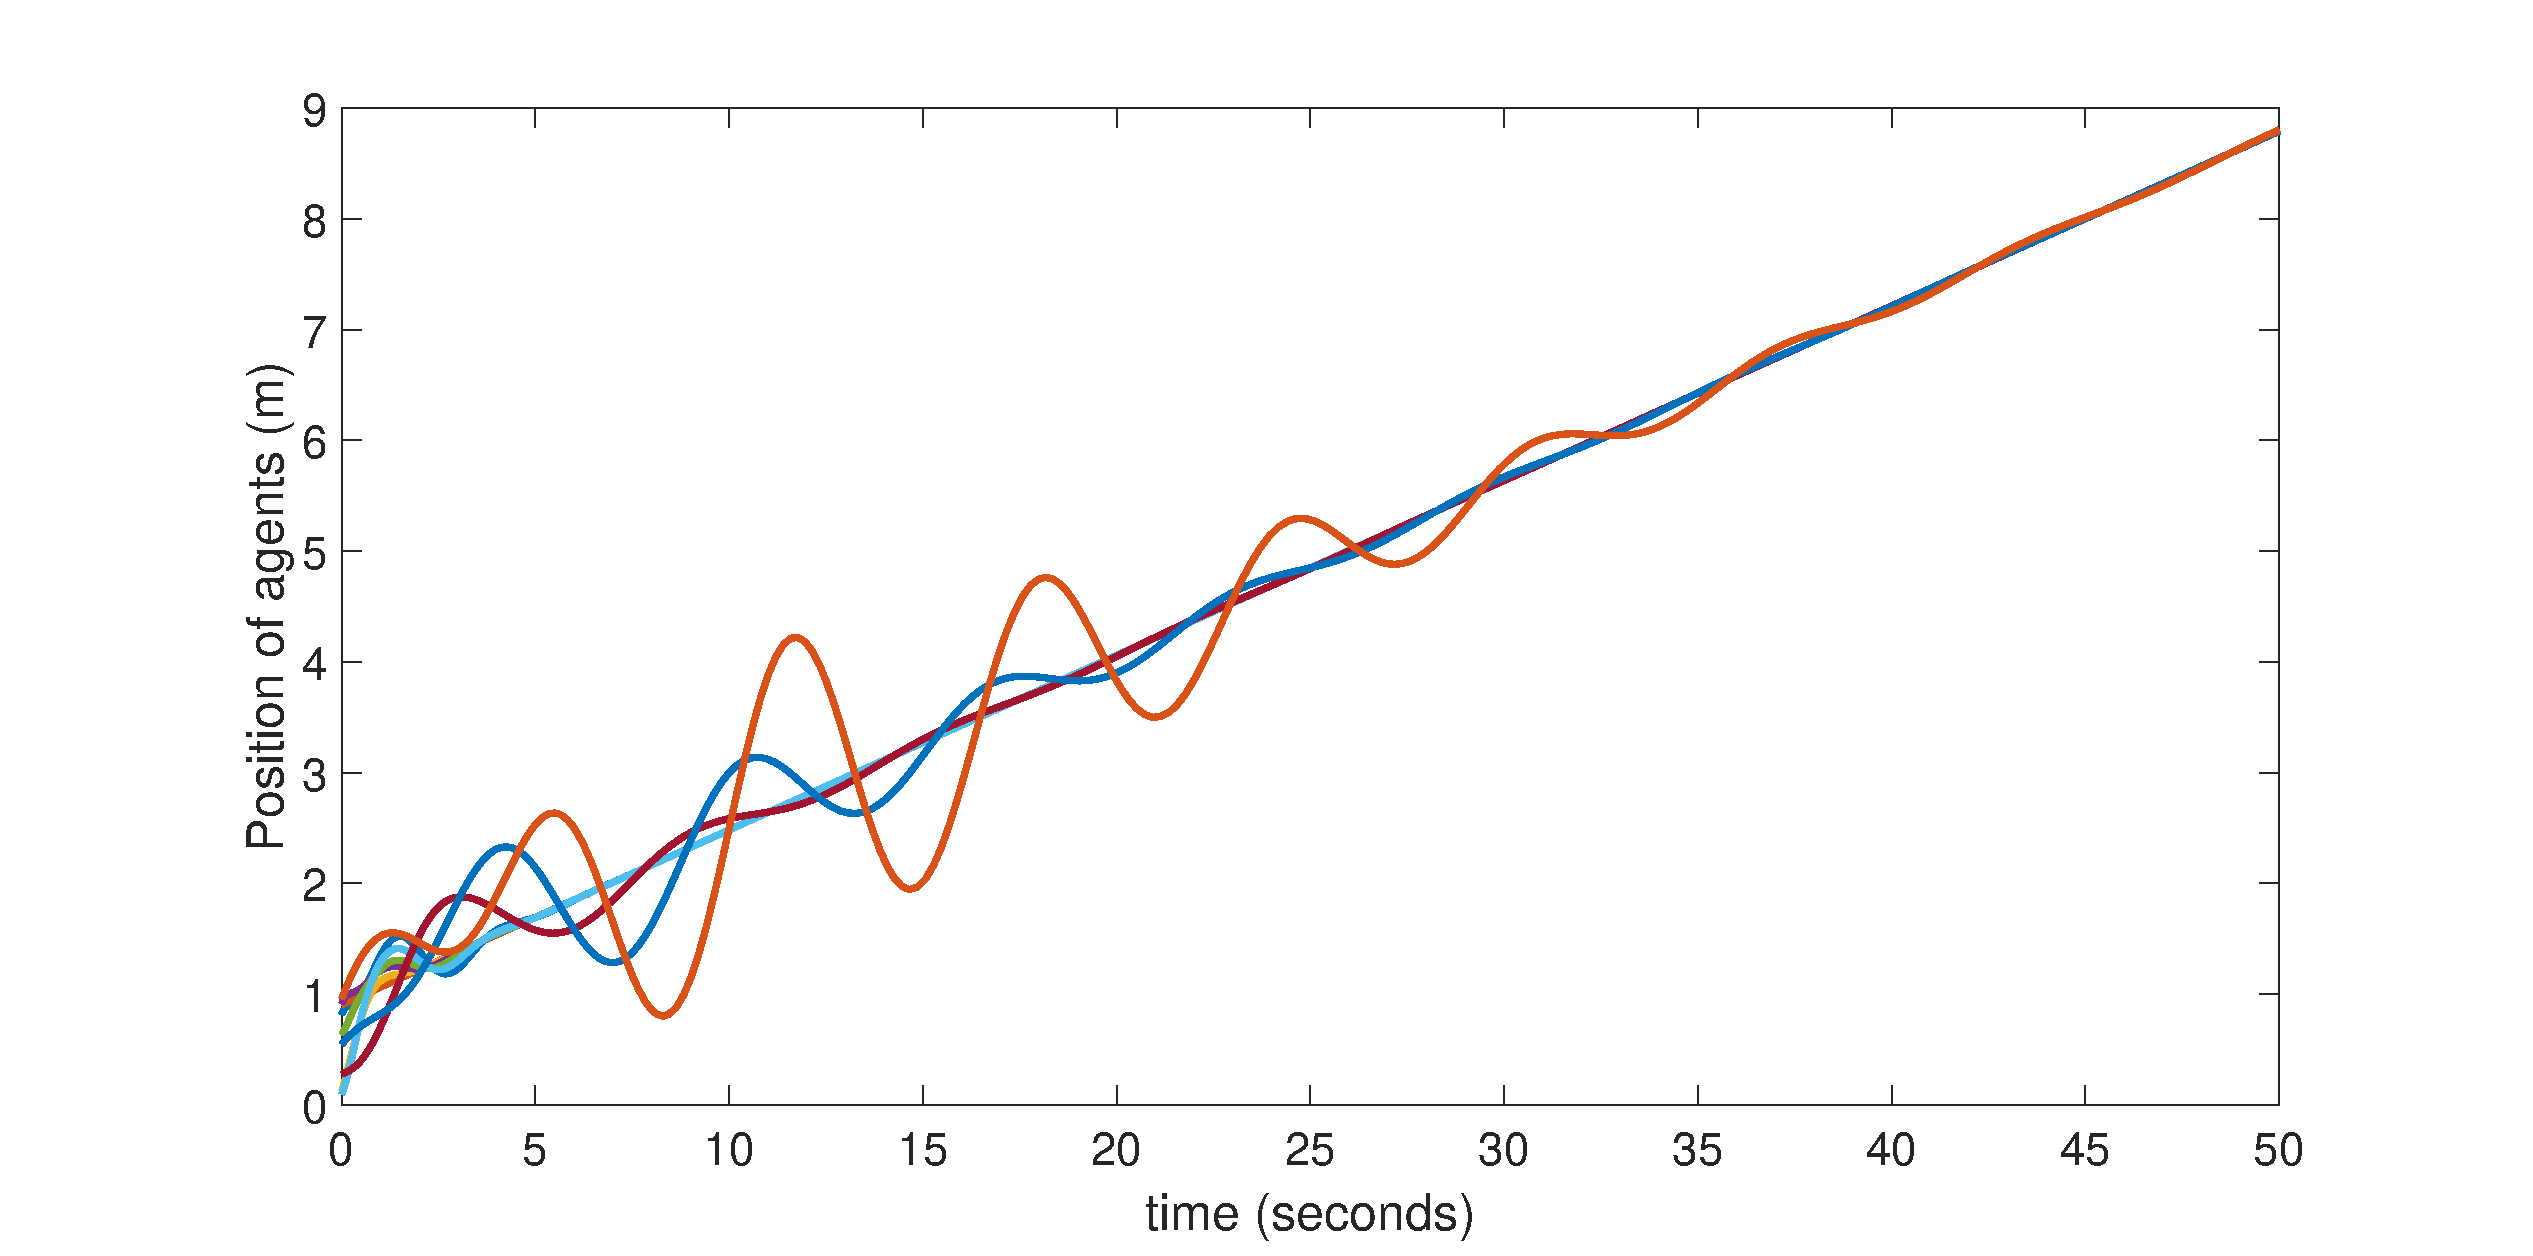
\includegraphics[scale=0.18,keepaspectratio]{Images/9-6-1_RootLocusLaplacianGamma0.4PositionConsensus1.eps}
				\caption{Position consensus with root locus based Laplacian design for $\gamma = 0.4$}
				\label{RootLocusBasedLaplacianPositionConsensus0.4}
			\end{figure}
		\end{column}
	\end{columns}
	%	Parameters chosen based on root locus tuning\\
	%	\begin{minipage}{0.45\linewidth}
		
		%\vspace{-0.3cm}    
		%	\end{minipage}
	%	\hspace{1em}
	%	\begin{minipage}{0.45\linewidth}
		%\vspace{-0.4cm}   
		
		%	\end{minipage}
	%\vspace{-1cm}
	\hyperlink{RLSimbase}{\beamerbutton{Back}}
\end{subframe}
%%%%%%%%%%%%%%%%%%%%%%%%%%%%%%%%%%%%%%%%%%%%%%%%%%%%%%%%%%%%%%%%%%%%%%%%%%%%%%%%%%%%%%%


\begin{subframe}{Gershgorin's Disc Theorem}\label{gers}
	%\begin{minipage}[]{0.4\textwidth}
	\begin{columns}
		\begin{column}{0.5\textwidth}
			Let there be a square matrix $A \in \mathbb{R}^{n \times n}$ and $$R_j(A)=\sum_{i=1,j \neq i}^{i=n}|a_{ij}| \text{ , } \forall \text{ }j \in \{1,2,\dots,n\}$$ $R_j(A)$ is the absolute sum of all the elements except the $j^{\rm th}$ element of column $j$ of matrix $A$. Consider a disc, say $\mathfrak{D}_j$, known as Gershgorin's disc for column $j$, given by $$\mathfrak{D}_j=\{r \in \mathbb{C}:|r-a_{jj}| \leq R_j(A)\}.$$
			Then, the eigenvalues of $A$ lies inside union of all the disks such that $D(A):=\bigcup_{j=1}^{n}\mathfrak{D}_j$.\\
		\end{column}
		\begin{column}{0.5\textwidth}
			\centering	
			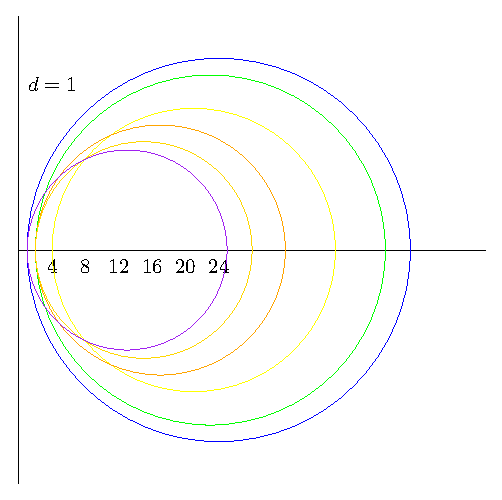
\includegraphics[scale=0.6,keepaspectratio]{Images/GershgorinDiscNotinAP.eps}\\
		\end{column}
	\end{columns}
	%	Let there be a square matrix $A \in \mathbb{R}^{n \times n}$ and $$R_j(A)=\sum_{i=1,j \neq i}^{i=n}|a_{ij}| \text{ , } \forall \text{ }j \in \{1,2,\dots,n\}$$ $R_j(A)$ is the absolute sum of all the elements except the $j^{\rm th}$ element of column $j$ of matrix $A$. Consider a disc, say $\mathfrak{D}_j$, known as Gershgorin's disc for column $j$, given by $$\mathfrak{D}_j=\{r \in \mathbb{C}:|r-a_{jj}| \leq R_j(A)\}.$$
	%	Then, the eigenvalues of $A$ lies inside union of all the disks such that $D(A):=\bigcup_{j=1}^{n}\mathfrak{D}_j$.\\
	%\end{minipage}
	%\begin{minipage}[]{0.5\textwidth}
	%	\centering	
	%	\includegraphics[scale=0.6,keepaspectratio]{GershgorinDiscNotinAP.eps}\\
	%\end{minipage}
	\textbf{Note: }Also true if the \textcolor{blue}{columns and rows are interchanged} since $A$ and $A^T$ have same eigenvalues.	\\
	\hyperlink{gersback}{\beamerbutton{Back}}
\end{subframe}
%\section{\color{blue}{Effect of Cycles on $\mathcal{H}_2$ performance of Double Integrators}}
%%%%%%%%%%%%%%%%%%%%%%%%%%%%%%%%%%%%%%%%%%%%%%%%%%%%%
\begin{comment}
\begin{frame}{Motivation: The Double Integrator Consensus}
	\vspace{-0.2cm}
	\begin{block}{}
			\textcolor{blue}{The system:}\vspace{-0.3cm} $$\dot{x}_i(t)=v_i(t),~~\dot{v}_i(t)=u_i(t)$$
		\textcolor{blue}{The proposed control law \footnotemark[1]} :
		$u_i(t)=-\sum_{j=1}^{N}{w_{ij}[(x_j(t)-x_i(t))}+\gamma{(v_j(t)-v_i(t))}],$
		
		where $x_i(t),v_i(t)\in \Rp$ denotes position and velocity of the $i^{th}$ agent in a $p$ dimensional space. $w_{ij}$ is the $(i,j)^{\rm th}$ entry of weighted adjacency matrix, and $\gamma$ is called the \textbf{velocity coupling factor}
	\end{block}
\vspace*{-0.2cm}
\begin{block}{}
		Double integrator consensus is achieved if :
	\begin{itemize}
		\item Network has a \emph{spanning tree }for undirected and directed network. [Necessary but not Sufficient]
		\item  $\gamma >0$ for undirected and $\gamma > \max_{i=2,\dots,n}\frac{\Im(\mu_i)}{|\mu_i|\sqrt{{\Re(\mu_i)}}}$for directed network. [Necessary \& Sufficient]~\footnotemark[2]
	\end{itemize}
	where, $\mu_i$, are the non-zero eigenvalues of $\mathcal{L}_n$, where $\Re(.)$ and $\Im(.)$ are the real and imaginary parts respectively.
\end{block}
	%\textcolor{blue}{Consensus} among double integrator, for any initial condition, is defined as:
	\vspace{-0.2cm}
	%\begin{equation*}\label{SecondConsensus}
	%	\begin{array}{ll}
	%		\lim_{t \rightarrow \infty}||x_i(t)-x_j(t)||=0,~~
	%		\lim_{t \rightarrow \infty}||v_i(t)-v_j(t)||=0, ~~ i,j \in \{1,2,\dots,N\}\\
	%	\end{array}
	%\end{equation*}
	%where 
	%\vspace{-0.6cm}
				%\vspace{-0.3cm}
			%\end{equation*}

	%\vspace{0.1cm}
	{\footnotetext[1]{\textcolor{blue}{Ren W, Atkins E}, {\em Second-order consensus protocols in multiple vehicle systems with local interactions}, AIAA guidance, navigation, and control conference and exhibit 2005.}}
	{\footnotetext[2]{\textcolor{blue}{Yu, Wenwu and Chen, Guanrong and Cao, Ming}, {\em Some necessary and sufficient conditions for second-order consensus in multi-agent dynamical systems}, Automatica 2010.}}	
\end{frame}

\end{comment}	
\begin{frame}[noframenumbering]
	\tableofcontents[currentsection]
	%\begin{center}
	%\textcolor{blue}{Problem 2: Effect of cycles on $\mathcal{H}_2$ performance of Double Integrators}
	%\end{center}
\end{frame}


%%%%%%%%%%%%%%%%%%%%%%%%%%%%%%%%%%%%%%%%%%%%%%%%%%%%
\begin{frame}{}
	\vspace{-0.1cm}
		The proposed control law under exogenous input such as node noise and edge noise can be represented as:\vspace{-0.2cm}
%	\vspace*{-0.3cm}
	\begin{equation*}
		u_i(t)=-\sum_{j=1}^{N}{w_{ij}[(x_j(t)-x_i(t))}+\gamma{(v_j(t)-v_i(t))}+r_{ij}(t)]+q_i(t),
	%	\vspace{-0.3cm}
	\end{equation*}
	where, $r_{ij}(t)$ is the edge/measurement noise and $q_i(t)$ is the node noise for $i^{th}$ agent. 
	\vspace{-0.1cm}
		\begin{block}{Noise Characterization}
		-- The node noise is an uncorrelated zero mean Gaussian noise such that $\mathbb{E}[q(t)q^T(t)]=\sigma_{q}^2I_n,$\\
		-- The edge noise is also an uncorrelated zero mean Gaussian noise $\mathbb{E}[r(t)r^T(t)]=\sigma_{r}^2I_e$\\
		where $q(t) \in \R^n$ and $r(t) \in \R^e$, $n,e$ are the number of nodes and edges in a graph and $I_n,I_e$ are identity matrices of dimension $n,e$.
	\end{block}
	\vspace*{-0.2cm}
	\pause
	\begin{block}{Problem Statement}
		Consider a \textcolor{blue}{chain/path of double integrators} following the above consensus protocol. Then,
		\begin{itemize}
			\item Characterize how an exogenous Gaussian noise propagates throughout a system and affect the energy of the monitored output.
			\item How these noises result in asymptotic deviation of each node's state from consensus state. 
			%\item Study effect of cycles on the $\mathcal{H}_2$ performance of the system in context to the combinatorial properties of graph such as cycles.
			%\item Characterize connection between combinatorial properties of graph and the dynamic properties of consensus protocol.
			\item And how does the cycles and $\gamma$ affect the performance of the system measured via the metric $\mathcal{H}_2$ norm.
		\end{itemize}
		%How does the various combinatorial properties of graph such as spanning trees and cycles impact the $\mathcal{H}_2$ performance of the system, in presence of exogenous inputs such as node (process) and edge(measurement) noises.}
		\end{block}
\end{frame}
%%%%%%%%%%%%%%%%%%%%%%%%%%%%%%%%%%%%%%%%%%%%%%%%%%%%
\begin{frame}		
\begin{block}{Literature}
	\begin{itemize}
		%\item Most of the work in the literature are on single integrator and undirected graph.
		\item Zelazo\footnotemark[1], through edge-based analysis, has explored the robustness concerning the combinatorial properties of graphs, albeit still within the context of single integrators and undirected topologies.
		\item The $\mathcal{H}_2$ analysis of networks under directed topology, has been studied by Young\footnotemark[2] for single integrators and by HG Oral\footnotemark[3] for double integrator, but with respect to spectral properties of graph.
		\item $\mathcal{H}_2$ analysis for undirected or directed topology for double integrators has not been explored in context to combinatorial properties of graph.
	\end{itemize}
\end{block}	
\begin{alertblock}{Challenges}
\begin{itemize}
%\item The asymmetrical structure of graph Laplacian in directed networks makes the analysis challenging. 
\item Existence of zero eigenvalues in the Laplacian makes the $\mathcal{H}_2$ norm unbounded.
\item Second Order topology adds further to the complexity.
\end{itemize}
\end{alertblock}
\vspace{0.1cm}
\footnotetext[1]{\textcolor{blue}{Zelazo, Daniel, Simone Schuler, and Frank Allgöwer.}, {\em "Performance and design of cycles in consensus networks." Systems \& Control Letters 62.1 (2013): 85-96.}}
\footnotetext[2]{\textcolor{blue}{Young, George Forrest, Luca Scardovi, and Naomi Ehrich Leonard.}, {\em "Robustness of noisy consensus dynamics with directed communication." Proceedings of the 2010 American Control Conference. IEEE, 2010.}}	
\footnotetext[3]{\textcolor{blue}{Giray Oral, H., Enrique Mallada, and Dennice F. Gayme.}, {\em "Performance of Single and Double-Integrator Networks over Directed Graphs." arXiv e-prints (2019): arXiv-1911.}} 
\end{frame}
%%%%%%%%%%%%%%%%%%%%%%%%%%%%%%%%%%%%%%%%%%%%%%%%%%%%
\begin{frame}{Node dynamics of system in Compact Form}
			\begin{figure}
				\centering
				%\includegraphics[scale=0.3]{blocknoise.png}
				%\includegraphics[trim={1cm 35cm 0cm 7cm},clip,scale=0.16]{block.jpg}
				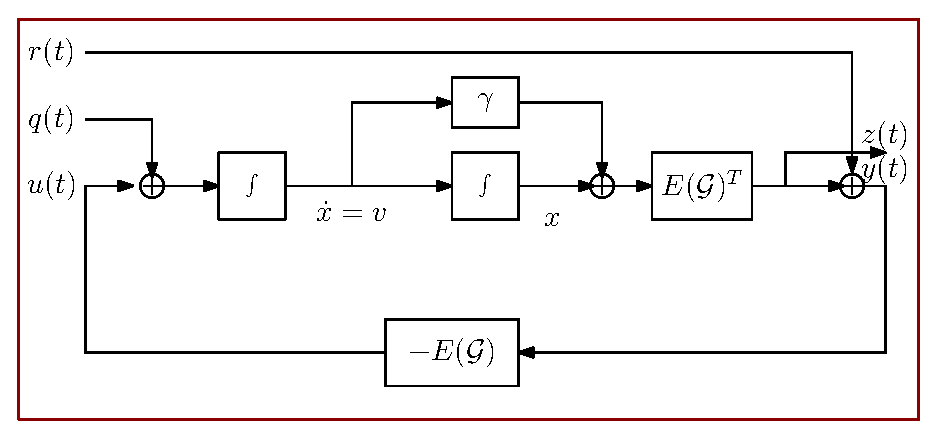
\includegraphics[scale=0.4]{Images/double_int_block_undirected.eps}
			\end{figure}
			\vspace*{-0.25cm}
			\begin{block}{Node Dynamics}
				The node dynamics where $z(t)$ is our monitored performance signal can be written as:
				$$\begin{bmatrix}
					\dot{x} \\ \dot{v}
				\end{bmatrix}=\begin{bmatrix}
					\mathbf{0} & I_n\\
					-\mathcal{L}_n & -\gamma \mathcal{L}_n
				\end{bmatrix}\begin{bmatrix}
					x \\ v
				\end{bmatrix}+
				\begin{bmatrix}
					\mathbf{0} & \mathbf{0}\\
					I_{n} & -E 
				\end{bmatrix}\begin{bmatrix}
					q \\ \r
				\end{bmatrix},~~z(t)=E^Tx(t)+\gamma E^T v(t)$$
				where, $\mathcal{L}_n=EE^T$ is the node Laplacian.
			\end{block}	
			where $x(t)=\begin{bsmallmatrix}x_1,x_2,\dots,x_n \end{bsmallmatrix}^T,v(t)=\begin{bsmallmatrix}v_1,v_2,\dots,v_n \end{bsmallmatrix}^T$ are the agent/node position and velocity vectors,\\
			$q(t)=\begin{bsmallmatrix}q_1,q_2,\dots,q_n \end{bsmallmatrix}^T$ is the node noise and $r(t)=\begin{bsmallmatrix}r_1,r_2,\dots,r_e \end{bsmallmatrix}^T$ is the edge noise
\end{frame}
%%%%%%%%%%%%%%%%%%%%%%%%%%%%%%%%%%%%%%%%%%%%%%%%%%%%
\begin{frame}
	\begin{figure}
		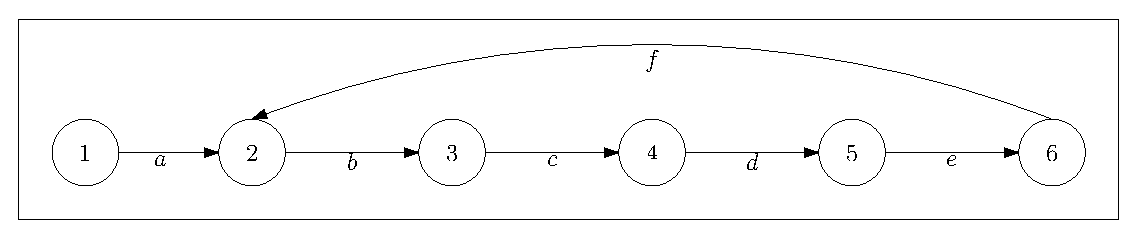
\includegraphics[scale=0.4]{Images/example_network.eps}		\\
	\end{figure}
	%\vspace{1mm}
	\begin{defi}[Incidence Matrix{\footnotemark[1]}]
		The incidence matrix for an oriented graph is defined such that $E(\mathcal{G})_{ij}=+1$ if edge $e_j$ is outgoing from vertex $i$, and $E(\mathcal{G})_{ij}=-1$ if edge $e_j$ is incoming at vertex $i$ and $E(\mathcal{G})_{ij}=0$ otherwise.
	\end{defi}
	%	\pause
	%\begin{block}{Incidence Matrix}
	\vspace{1mm}
	$$E=\begin{bsmallmatrix}
		1 &  0 &  0 &  0 &  0 & \color{cyan}{0} \\
		-1 &  1 &  0 &  0 &  0 & \color{cyan}{-1} \\
		0 & -1 &  1 &  0 &  0 & \color{cyan}{0} \\
		0 &  0 & -1 &  1 &  0 & \color{cyan}{0} \\
		0 &  0 &  0 & -1 &  1 & \color{cyan}{0} \\
		0 &  0 &  0 &  0 & -1 & \color{cyan}{1} \\
	\end{bsmallmatrix}=\begin{bmatrix}\etree & \color{cyan}{E_c}\end{bmatrix}=\etree \begin{bmatrix} I & \color{cyan} T \end{bmatrix}=\etree R$$ 
	where $T=\begin{bmatrix}0 & -1 & -1 & -1 & -1 \end{bmatrix}^T$ and
	$T=(\etree^T\etree)^{-1}\etree^TE_c$
	\\
	\footnotetext[1]{D. Zelazo, Amirreza Rahmani and Mehran Mesbahi, "Agreement via the edge laplacian," 2007 46th IEEE Conference on Decision and Control, New Orleans, LA, USA, 2007, pp. 2309-2314.}
\end{frame}
\begin{frame}
		\begin{defi}[Edge Laplacian of a graph]
		The edge Laplacian for an undirected graph is defined as:  $$\mathcal{L}_{e}:= E^TE,~~~~\letree:= E_\tau^T \etree$$
		where $\mathcal{L}_{e} \in \R^{e \times e}$, $\letree \in \R^{(n-1) \times (n-1)}$
	\end{defi}
			\begin{lemma}[Separation of zero eigenvalue{\footnotemark[1]}]
				Node Laplacian $\mathcal{L}_{n}=EE^T$ for a connected graph $\mathcal{G}$ is similar to $\begin{bmatrix}
					\letree {R}R^T & \textbf{0} \\
					\textbf{0} & 0
				\end{bmatrix}$
			\end{lemma}	
			Proof Outline: Define $S_v=\begin{bmatrix}
				\etree(E_{\tau}^T\etree)^{-1} & \mathbf{1}
			\end{bmatrix}$, thus, $S_v^{-1}=\begin{bmatrix}
				E_{\tau}^T & (1/n)\mathbf{1}^T \end{bmatrix}^T$. Apply the transformation $S_v^{-1}\mathcal{L}_{n}S_v$.					
	\begin{alertblock}{}
		\begin{itemize}
			\item $\letree {R}R^T$ is known as essential edge Laplacian.
			\item Although $\letree$ and $RR^T$ are symmetric matrices, essential edge Laplacian is an asymmetric matrix.
		\end{itemize}
	\end{alertblock}
		\footnotetext[1]{D. Zelazo, Amirreza Rahmani and Mehran Mesbahi, "Agreement via the edge laplacian," 2007 46th IEEE Conference on Decision and Control, New Orleans, LA, USA, 2007, pp. 2309-2314.}
\end{frame}
%%%%%%%%%%%%%%%%%%%%%%%%%%%%%%%%%%%%%%%%%%%%%%%%%%%%

\begin{frame}
	%Transforming the node states to edge states:\\
	%$\dot{X}_e=\begin{bmatrix}
		%	0 & I\\
		%	-E^TE_{in} & -\gamma E^TE_{in}
		%\end{bmatrix}X_e+\begin{bmatrix}
		%	0 & 0\\
		%	E^T & -E^TE_{in} 
		%\end{bmatrix}N(t)$\\
		%where,\\
		%$X=\begin{bmatrix}
			%	x(t) & v(t)
			%\end{bmatrix}^T,X_e=\begin{bmatrix}
			%	x_e(t) & v_e(t)
			%\end{bmatrix}^T,$\\
			%$N=\begin{bmatrix}
				%	q(t) & r(t)
				%\end{bmatrix}^T$,
				%$q(t) \in \R^{n},~~r(t) \in \R^{|e|}$\\
					\begin{lemma}[Coordinate Transformation]
					Using $S_v=\begin{bmatrix}
						\etree(E_{\tau}^T\etree)^{-1} & \mathbf{1}
					\end{bmatrix}$ and applying the coordinate transformation $\begin{bmatrix} S_v & \mathbf{0} \\ \mathbf{0} & S_v \end{bmatrix}\begin{bmatrix} x_e \\ v_e \end{bmatrix}=\begin{bmatrix} x \\ v \end{bmatrix}$, Node states are transformed to new states $x^T_e=\begin{bmatrix*} x^T_{\tau} & x^T_{\mathbf{1}}\end{bmatrix*}^T$, and $v^T_e=\begin{bmatrix*} v^T_{\tau} & v^T_{\mathbf{1}}\end{bmatrix*}^T$
					
					where, $x_\tau,v_\tau \in \R^{n-1}$ are relative state information across the spanning trees and $x_{\mathbf{1}}, v_{\mathbf{1}} \in \R$ are mode in the agreement subspace. 
				\end{lemma}	
				\begin{block}{Reduced Order Edge Dynamics}
					 Using the above coordinate transformation and considering ${X}_{e_\tau}=\begin{bmatrix}
					 	x_\tau^T & v_\tau^T \end{bmatrix}^T$, the reduced order system ($\Sigma_{\tau}$) can be represented as:
					$$\dot{X}_{e_\tau}=\begin{bmatrix}
						\mathbf{0} & I_{n-1}\\
						-\letree RR^T & -\gamma\letree RR^T
					\end{bmatrix}X_{e_\tau}+\begin{bmatrix}
						\mathbf{0} & \mathbf{0}\\
						\sigma_{q}E_{\tau}^T & -\sigma_{r}\letree R
					\end{bmatrix}\hat{N}(t)$$
					$$z(t)=X_{e_\tau}$$
					where, ${X}_{e_\tau} \in \R^{2(n-1)},~\hat{N}(t) \in \R^{(n+|e|)} $ is the normalized noise signal.
				\end{block}
			\end{frame}
\begin{frame}{}
	\begin{defi}[$\mathcal{H}_2$ Norm{\footnotemark[1]}]
		Consider a transfer function $G(s)=\left[
		\begin{array}{c|c}
			A & B \\
			\hline
			C & 0
		\end{array}
		\right]$
		with $A$ stable. Then we have $$\norm{G}_2^2=trace(B^*QB)=trace(CPC^*)$$
		where $Q$ and $P$ are observability and controllability gramians that can be obtained from the following Lyapunov equation:
		$$A^*Q+QA+C^*C=0;~~AP+PA^*+BB^*=0 $$
	\end{defi}
	\pause
	\begin{block}{$\mathcal{H}_2$ norm}
		The $\mathcal{H}_2$ Norm of the system $\Sigma_{\tau}$, where, $A=\begin{bmatrix}
			\mathbf{0} & I_{n-1}\\
			-\letree RR^T & -\gamma\letree RR^T
		\end{bmatrix}$, $B=\begin{bmatrix}
			\mathbf{0} & \mathbf{0}\\
			\sigma_{q}E_{\tau}^T & -\sigma_{r}\letree R
		\end{bmatrix}$ and $C=I_{n-1}$ is given by $$\norm{\Sigma_{\tau}}_2^2=trace(P)$$
		where $P$ is the solution to the Lyapunov equation $AP+PA^T+BB^T=0,$
	\end{block}							
	\footnotetext[1]{Zhou, Kemin, and John Comstock Doyle. Essentials of robust control. Vol. 104. Upper Saddle River, NJ: Prentice hall, 1998.}
\end{frame}

%%%%%%%%%%%%%%%%%%%%%%%%%%%%%%%%%%%%%%%%%%%%%%%%%%%%
\begin{comment}
\begin{frame}{$\mathcal{H}_2$ Norm of the System $\Sigma_{\tau}$}
	Let $P=\begin{bmatrix}
		P_1 & P_2\\
		P_2^T & P_3
	\end{bmatrix}$, $A_3 = -\letree{R}R^T$, and $QQ^T = \sigma_{r}^2 \letree{R}{R}^T\letree^T + \sigma_{q}^2 \etree^T \etree$, \\
	Thus, the Lyapunov equation reduces to the following set of equations:
	\begin{equation*}
		P_2^T = -P_2
	\end{equation*}
	\begin{equation*}
		P_3 + P_1 A_3^T + \gamma P_2 A_3^T = 0
	\end{equation*}
	\begin{equation*}
		P_3 + A_3 P_1 + \gamma A_3 P_2^T = 0
	\end{equation*}
	\begin{equation*}
		A_3 P_2 + P_2^T A_3^T + \gamma A_3 P_3 + \gamma P_3 A_3^T = -QQ^T
	\end{equation*}
	\pause
	Let $\color{blue}J=2\gamma\left[2\gamma^2(I_{n-1} \otimes A_3 + A_3 \otimes I_{n-1}) + 2I_{(n-1)^2} - (A_3^{-1} \otimes A_3 + A_3 \otimes A_3^{-1})\right]^{-1}$, then, solving yields:
	$$\color{magenta}\text{vec}(P_3) = J\text{vec}(-QQ^T)$$
	\vspace{-0.2cm}
	$$\color{magenta}\text{vec}(P_1) = \frac{-1}{2}(I_{n-1} \otimes A_3^{-1} + A_3^{-1} \otimes I_{n-1})\text{vec}(P_3)$$
	\vspace{-0.2cm}
	%$$\color{magenta}\text{vec}(P_2) = \frac{1}{2\gamma}(I \otimes A_3^{-1} - A_3^{-1} \otimes I)\text{vec}(P_3)$$
	\pause
	and hence, the $\mathcal{H}_2$ norm of the system is:
	$$\color{cyan}\|\Sigma_{\tau}\|_2^2 = \text{trace}(P) = \text{trace}(P_1) + \text{trace}(P_3)$$
\end{frame}

\end{comment}
%%%%%%%%%%%%%%%%%%%%%%%%%%%%%%%%%%%%%%%%%%%%%%%%%%%%
\begin{frame}{$\mathcal{H}_2$ Norm for Network of Double Integrators}
	\vspace{-0.2cm}
\begin{myblock}{Theorem 1}
	The $\mathcal{H}_2$ Norm of System $\Sigma_{\tau}$ is 
	$$\norm{\Sigma_{\tau}}^2=\frac{1}{2\gamma}\text{ trace}[(I_{n-1}-A_3^{-1})\color{cyan}{(\sigma_r^2I_{n-1}-\sigma_q^2A_3^{-1})\letree}]$$
	where, $A_3 = -\letree{R}R^T$
\end{myblock}
\textbf{Note:} 
\begin{itemize}
	\item A double integrator network always has a poorer performance than a single integrator.
	\item Norm for double integrator depends on choice of spanning trees unlike single integrator.
\end{itemize}
	\begin{block}{Some Important Properties}
	For an undirected path graph: ($E=\begin{bmatrix}\etree & \color{cyan}{E_c}\end{bmatrix}=\etree \begin{bmatrix} I & \color{cyan} T \end{bmatrix}=\etree R$)
	\begin{itemize}
		\item $\text{trace}[\letree]=2(n-1)$ (True for any spanning tree)
		\item $\text{trace}[\letree^{-1}]=(n-1)(n+1)/6$
		%\item $(RR^T)^{-1}=(I+TT^T)^{-1}$ 
	\end{itemize}
\end{block}
\end{frame}
%%%%%%%%%%%%%%%%%%%%%%%%%%%%%%%%%%%%%%%%%%%%%%%%%%%%
\begin{frame}
	For a path graph with one cycle:
	\begin{itemize}
		\item $(RR^T)^{-1}=(I+TT^T)^{-1}=(I-TT^T/(\ell+1))$ (Matrix Inversion Lemma)
		\item $\text{ trace}[(RR^T)^{-1}]=n-2+1/(\ell+1)]$
		\item $\text{ trace}[(RR^T)^{-1}\letree^{-1}(RR^T)^{-1}]=\text{ trace}[\letree^{-1}-TT^T\letree^{-1}/(\ell+1)]$
	\end{itemize}
\vspace{-0.2cm}
\begin{myblock}{Theorem 2}
		Given an undirected path graph with $n$ node and presence of a cycle of length $\ell$, the $\mathcal{H}_2$ Norm of System $\Sigma_{\tau}$ is
		\vspace{-0.3cm}
		$$\norm{\Sigma_{\tau}}^2=\frac{1}{2\gamma}\left[\textcolor{violet}{2\sigma_r^2(n-1)}+\textcolor{magenta}{(\sigma_{q}^2+\sigma_r^2)(n-2+\frac{1}{\ell+1})}+\textcolor{cyan}{\sigma_q^2\text{ trace}[(RR^T)^{-1}\letree^{-1}(RR^T)^{-1}]}\right]$$
		$$\norm{\Sigma_{\tau}}^2=\frac{1}{2\gamma}\left[\textcolor{violet}{2\sigma_r^2(n-1)}+\textcolor{magenta}{(\sigma_{q}^2+\sigma_r^2)(n-2+\frac{1}{\ell+1})}+\textcolor{cyan}{\sigma_q^2\frac{(n-1)(n+1)}{6}-\sigma_q^2\text{ trace}[\frac{TT^T\letree^{-1}}{\ell+1}]}\right]$$
		where, $\ell=|j-i|$ is the length of cycle and $j,i$ are the end nodes of the edge forming the cycle.
	\end{myblock}
	\vspace{-0.3cm}
	\begin{alertblock}{}
		%$\mathcal{H}_2$ performance is:
		\begin{itemize}
			\item Larger cycle are better.
			\item Increased values of $\gamma$ leads to improvement in performance.
			\item Smaller network performs better than large networks.
		\end{itemize}
	\end{alertblock}
\end{frame}
%%%%%%%%%%%%%%%%%%%%%%%%%%%%%%%%%%%%%%%%%%%%%%%%%%%%
%%%%%%%%%%%%%%%%%%%%%%%%%%%%%%%%%%%%%%%%%%%%%%%%%%%%
\begin{frame}{$\mathcal{H}_2$ Norm of the system with varying cycle length in a network}
	%\vspace{-0.5cm}
	\begin{figure}
		%\hspace{-1cm}
		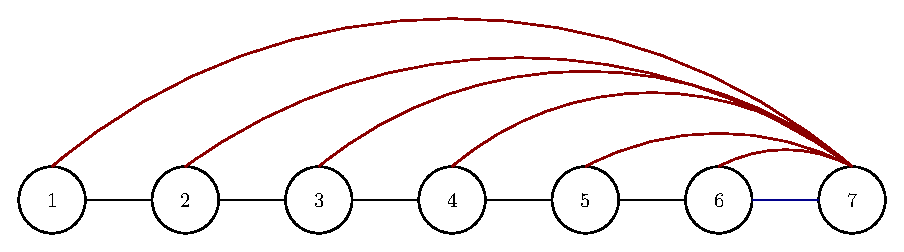
\includegraphics[scale=0.5]{Images/one_cycle_undirected.eps}
	\end{figure}
			%\vspace{-0.7cm}
			\begin{figure}
				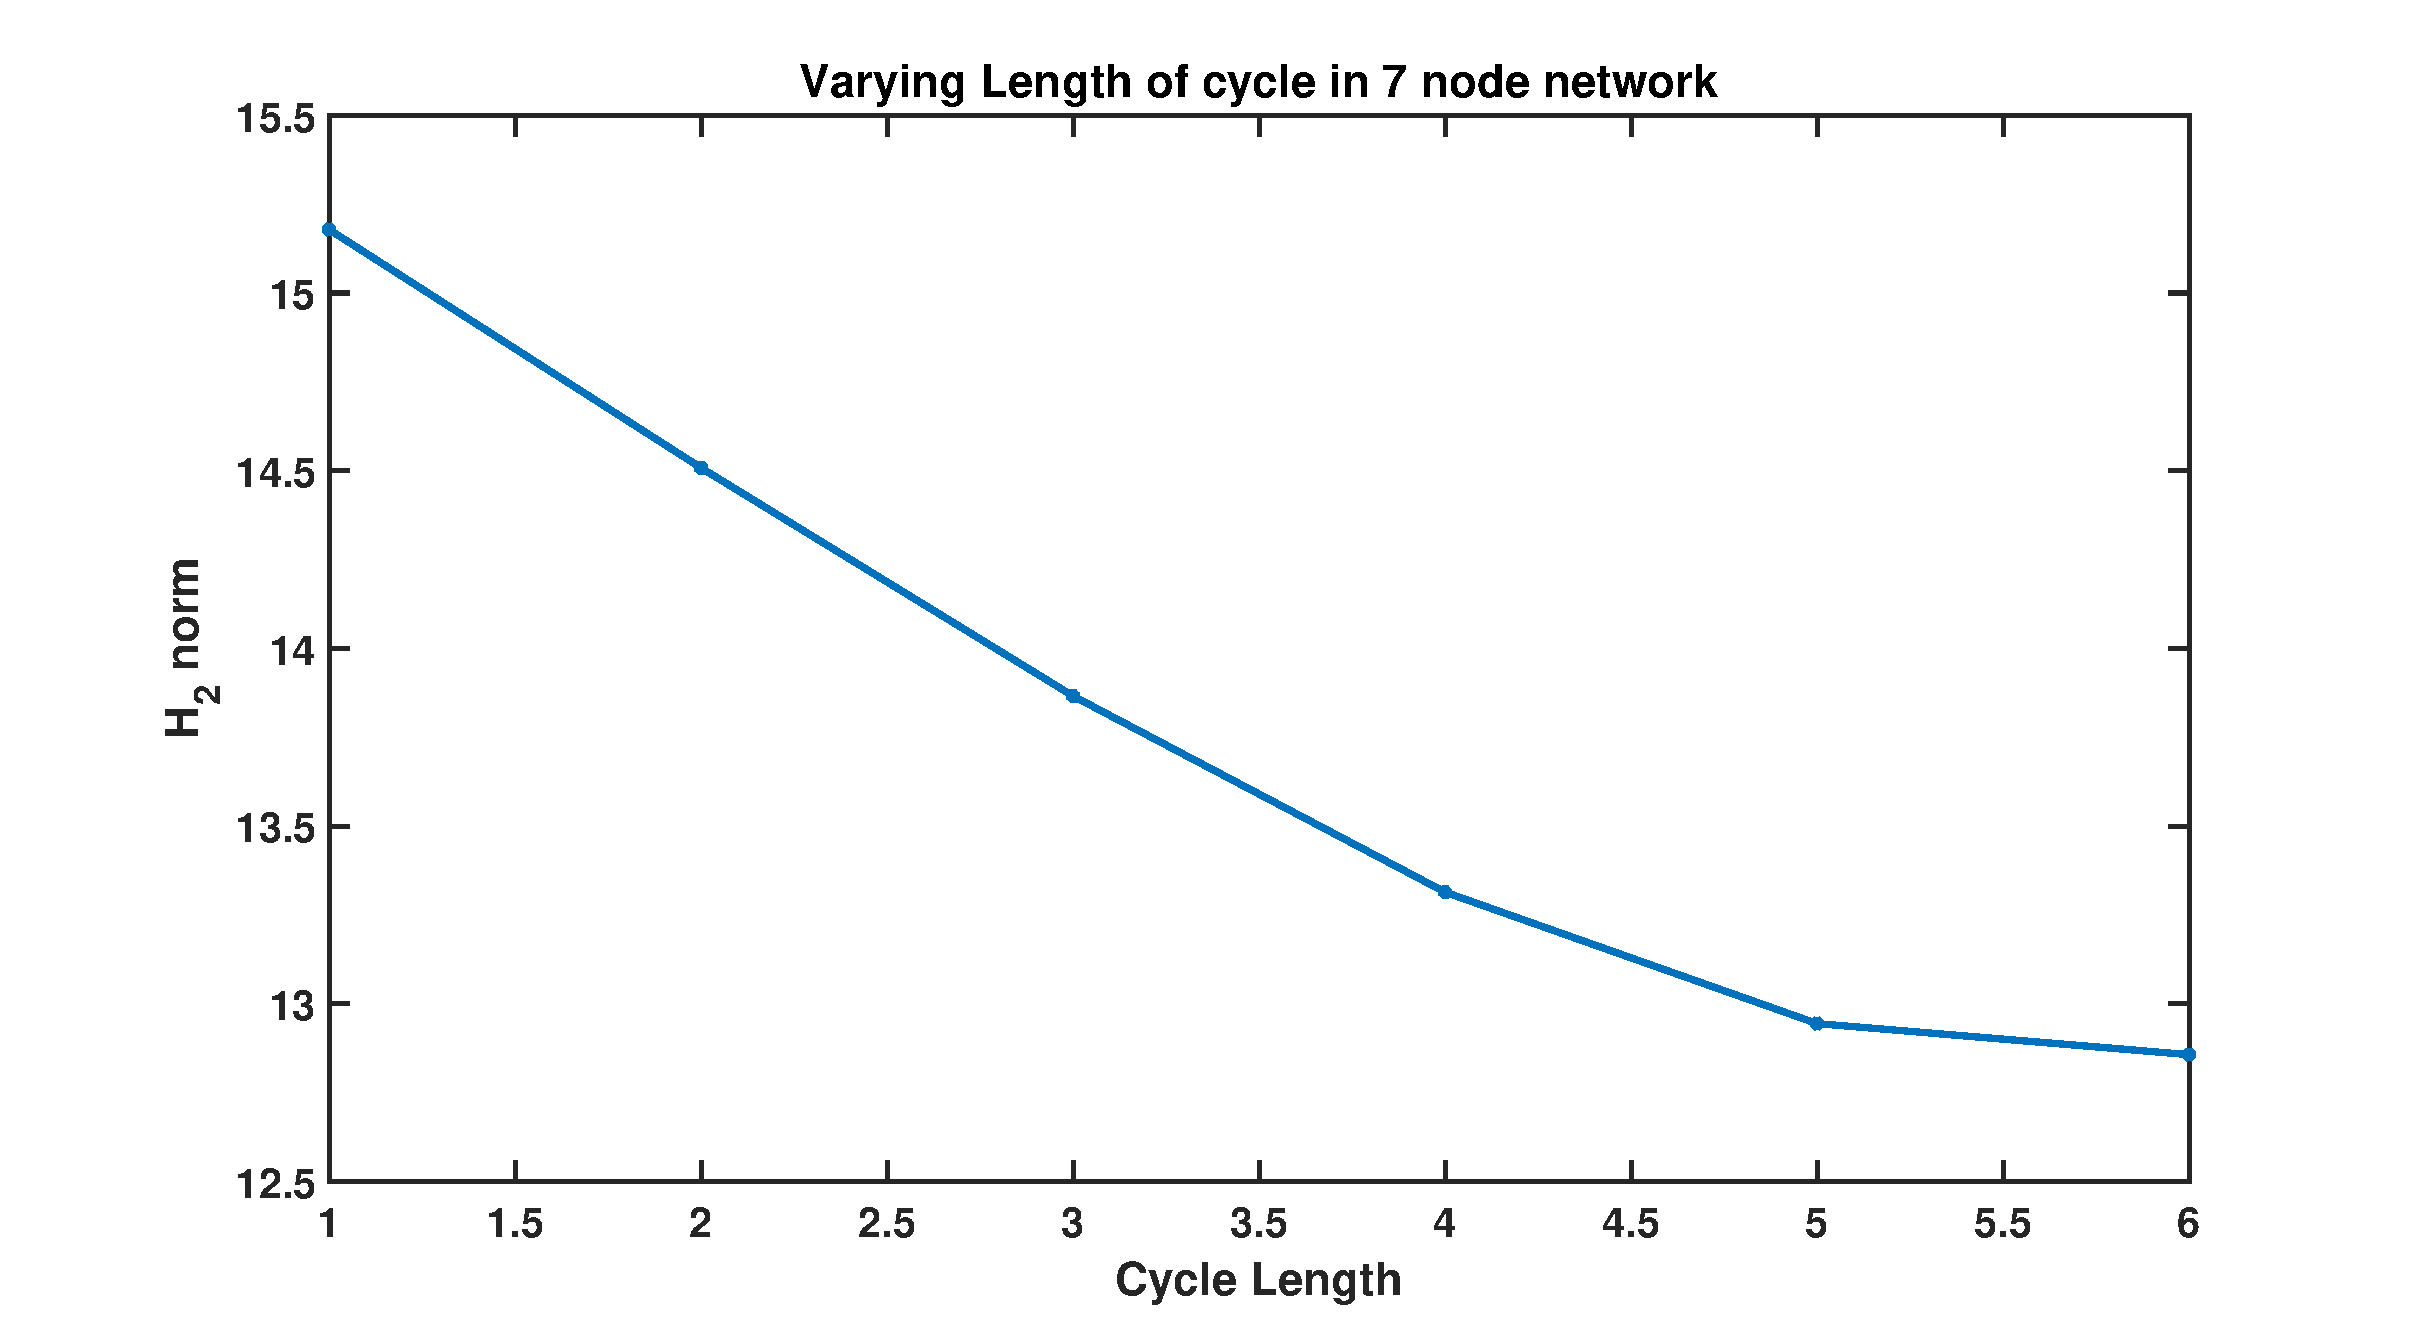
\includegraphics[scale=0.2]{Images/Single_Cycle_Varying_Length.eps}
			\end{figure}
\end{frame}
%%%%%%%%%%%%%%%%%%%%%%%%%%%%%%%%%%%%%%%%%%%%%%%%%%%%
\begin{frame}
		\begin{myblock}{Theorem 3}
		Given an undirected path graph on $n$ double integrators, addition of an edge that leads to the formation of a cycle of length $\ell < n $, results in $\mathcal{H}_2$ norm of a system $\Sigma_{\tau}$ is given by:
		$$\norm{\Sigma_{\tau}}^2=\frac{1}{2\gamma}\left[\textcolor{violet}{2\sigma_r^2(n-1)}+\textcolor{magenta}{(\sigma_{q}^2+\sigma_r^2)(n-2+\frac{1}{\ell+1})}+\textcolor{cyan}{\sigma_q^2\frac{(n-1)(n+1)}{6}-\frac{\sigma_q^2(\ell+2)}{(\ell+1)^2}\text{ trace}[TT^T\letree^{-1}]}\right]$$
	\end{myblock}
\vspace{-0.3cm}
\begin{alertblock}{}
	\begin{itemize}
\item For a cycle of length $\ell, ~~\text{trace}[TT^T\letree^{-1}]$ is maximum if the cycle is at the center of the tree.	
\end{itemize}
\end{alertblock}
\vspace{-0.5cm}
	$$TT^T=\begin{bmatrix}
		0 & 0 & 0 & 0 & 0 & 0 \\
		0 & 1 & 1 & 0 & 0 & 0 \\
		0 & 1 & 1 & 0 & 0 & 0 \\
		0 & 0 & 0 & 0 & 0 & 0 \\
		0 & 0 & 0 & 0 & 0 & 0 \\
		0 & 0 & 0 & 0 & 0 & 0 
	\end{bmatrix},~~\letree^{-1}=\begin{bmatrix}
	0.8571 & 0.7143 & 0.5714 & 0.4286 & 0.2857 & 0.1429 \\
	0.7143 & 1.4286 & 1.1429 & 0.8571 & 0.5714 & 0.2857 \\
	0.5714 & 1.1429 & 1.7143 & 1.2857 & 0.8571 & 0.4286 \\
	0.4286 & 0.8571 & 1.2857 & 1.7143 & 1.1429 & 0.5714 \\
	0.2857 & 0.5714 & 0.8571 & 1.1429 & 1.4286 & 0.7143 \\
	0.1429 & 0.2857 & 0.4286 & 0.5714 & 0.7143 & 0.8571 
	\end{bmatrix}$$
	$$\text{trace}[TT^T\letree^{-1}]=5.4286$$
\end{frame}
%%%%%%%%%%%%%%%%%%%%%%%%%%%%%%%%%%%%%%%%%%%%%%%%%%%%
\begin{frame}{$\mathcal{H}_2$ Norm of the system with cycle length in presence of single cycle}
	%\vspace{-0.5cm}
		\begin{figure}
		%\hspace{-1cm}
		\includegraphics[scale=0.5]{Images/same_length2_different_position_undirected.eps}
	\end{figure}
	\begin{columns}
		\begin{column}{0.5\textwidth}
			%\vspace{-0.7cm}
			\begin{figure}
				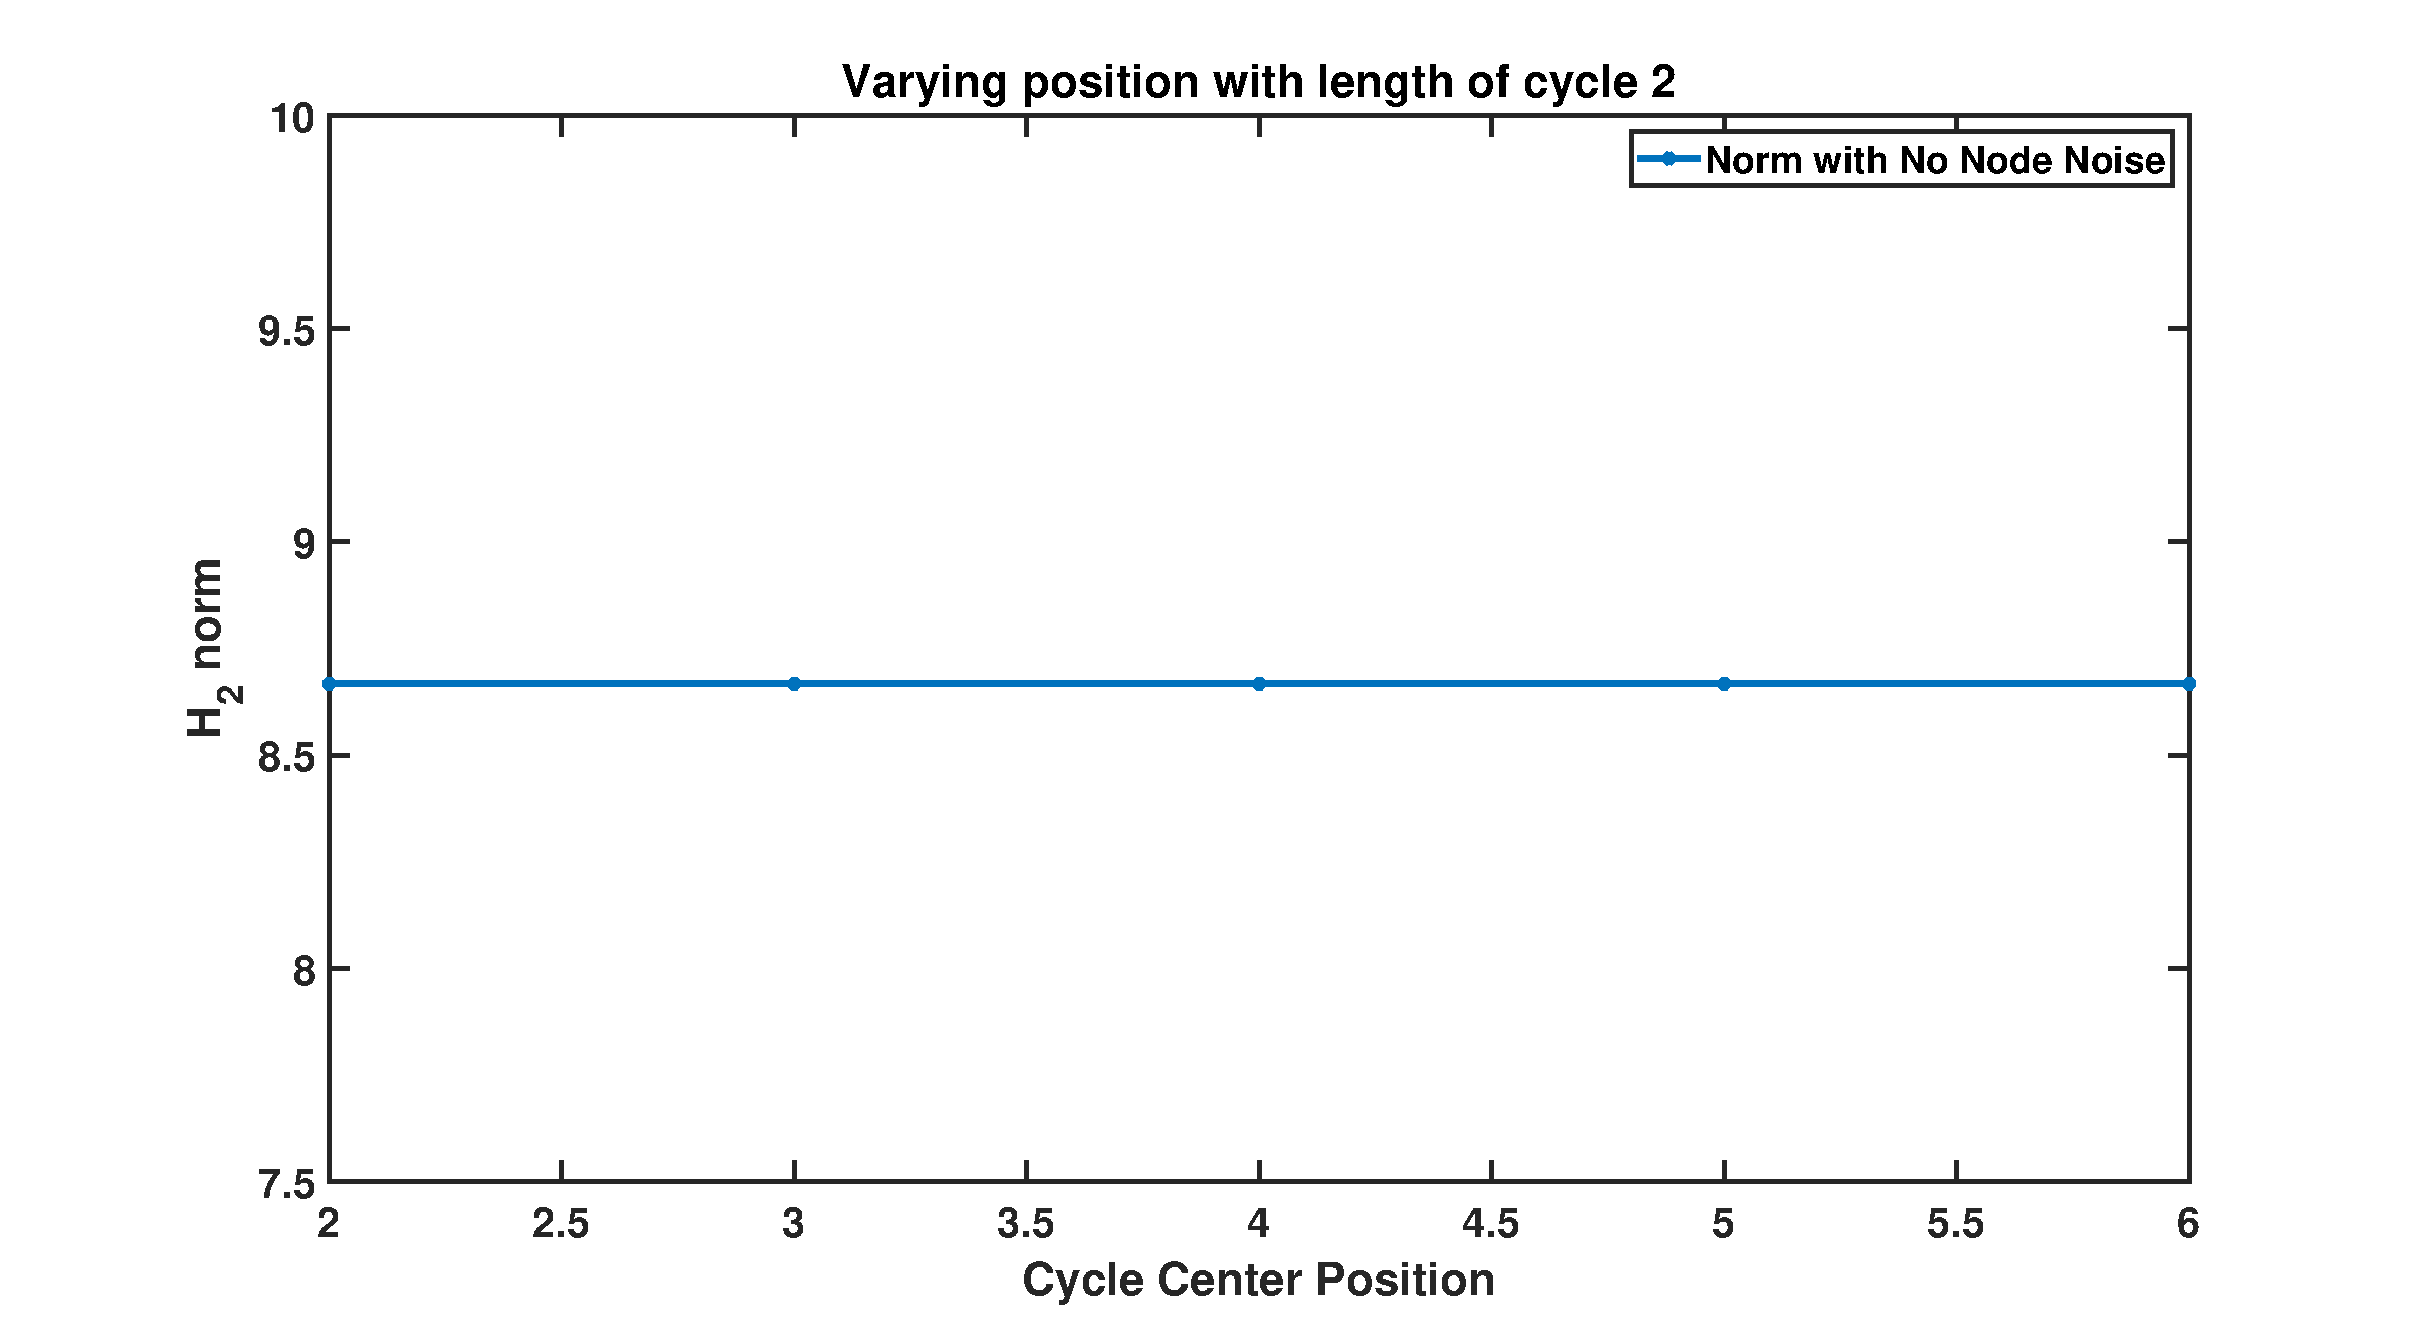
\includegraphics[scale=0.2]{Images/Single_Cycle_Length2_unidrected_Absent_Node_Noise.eps}
			\end{figure}
		\end{column}
		\begin{column}{0.5\textwidth}
			%\vspace{-0.7cm}
		\begin{figure}
				\centering
				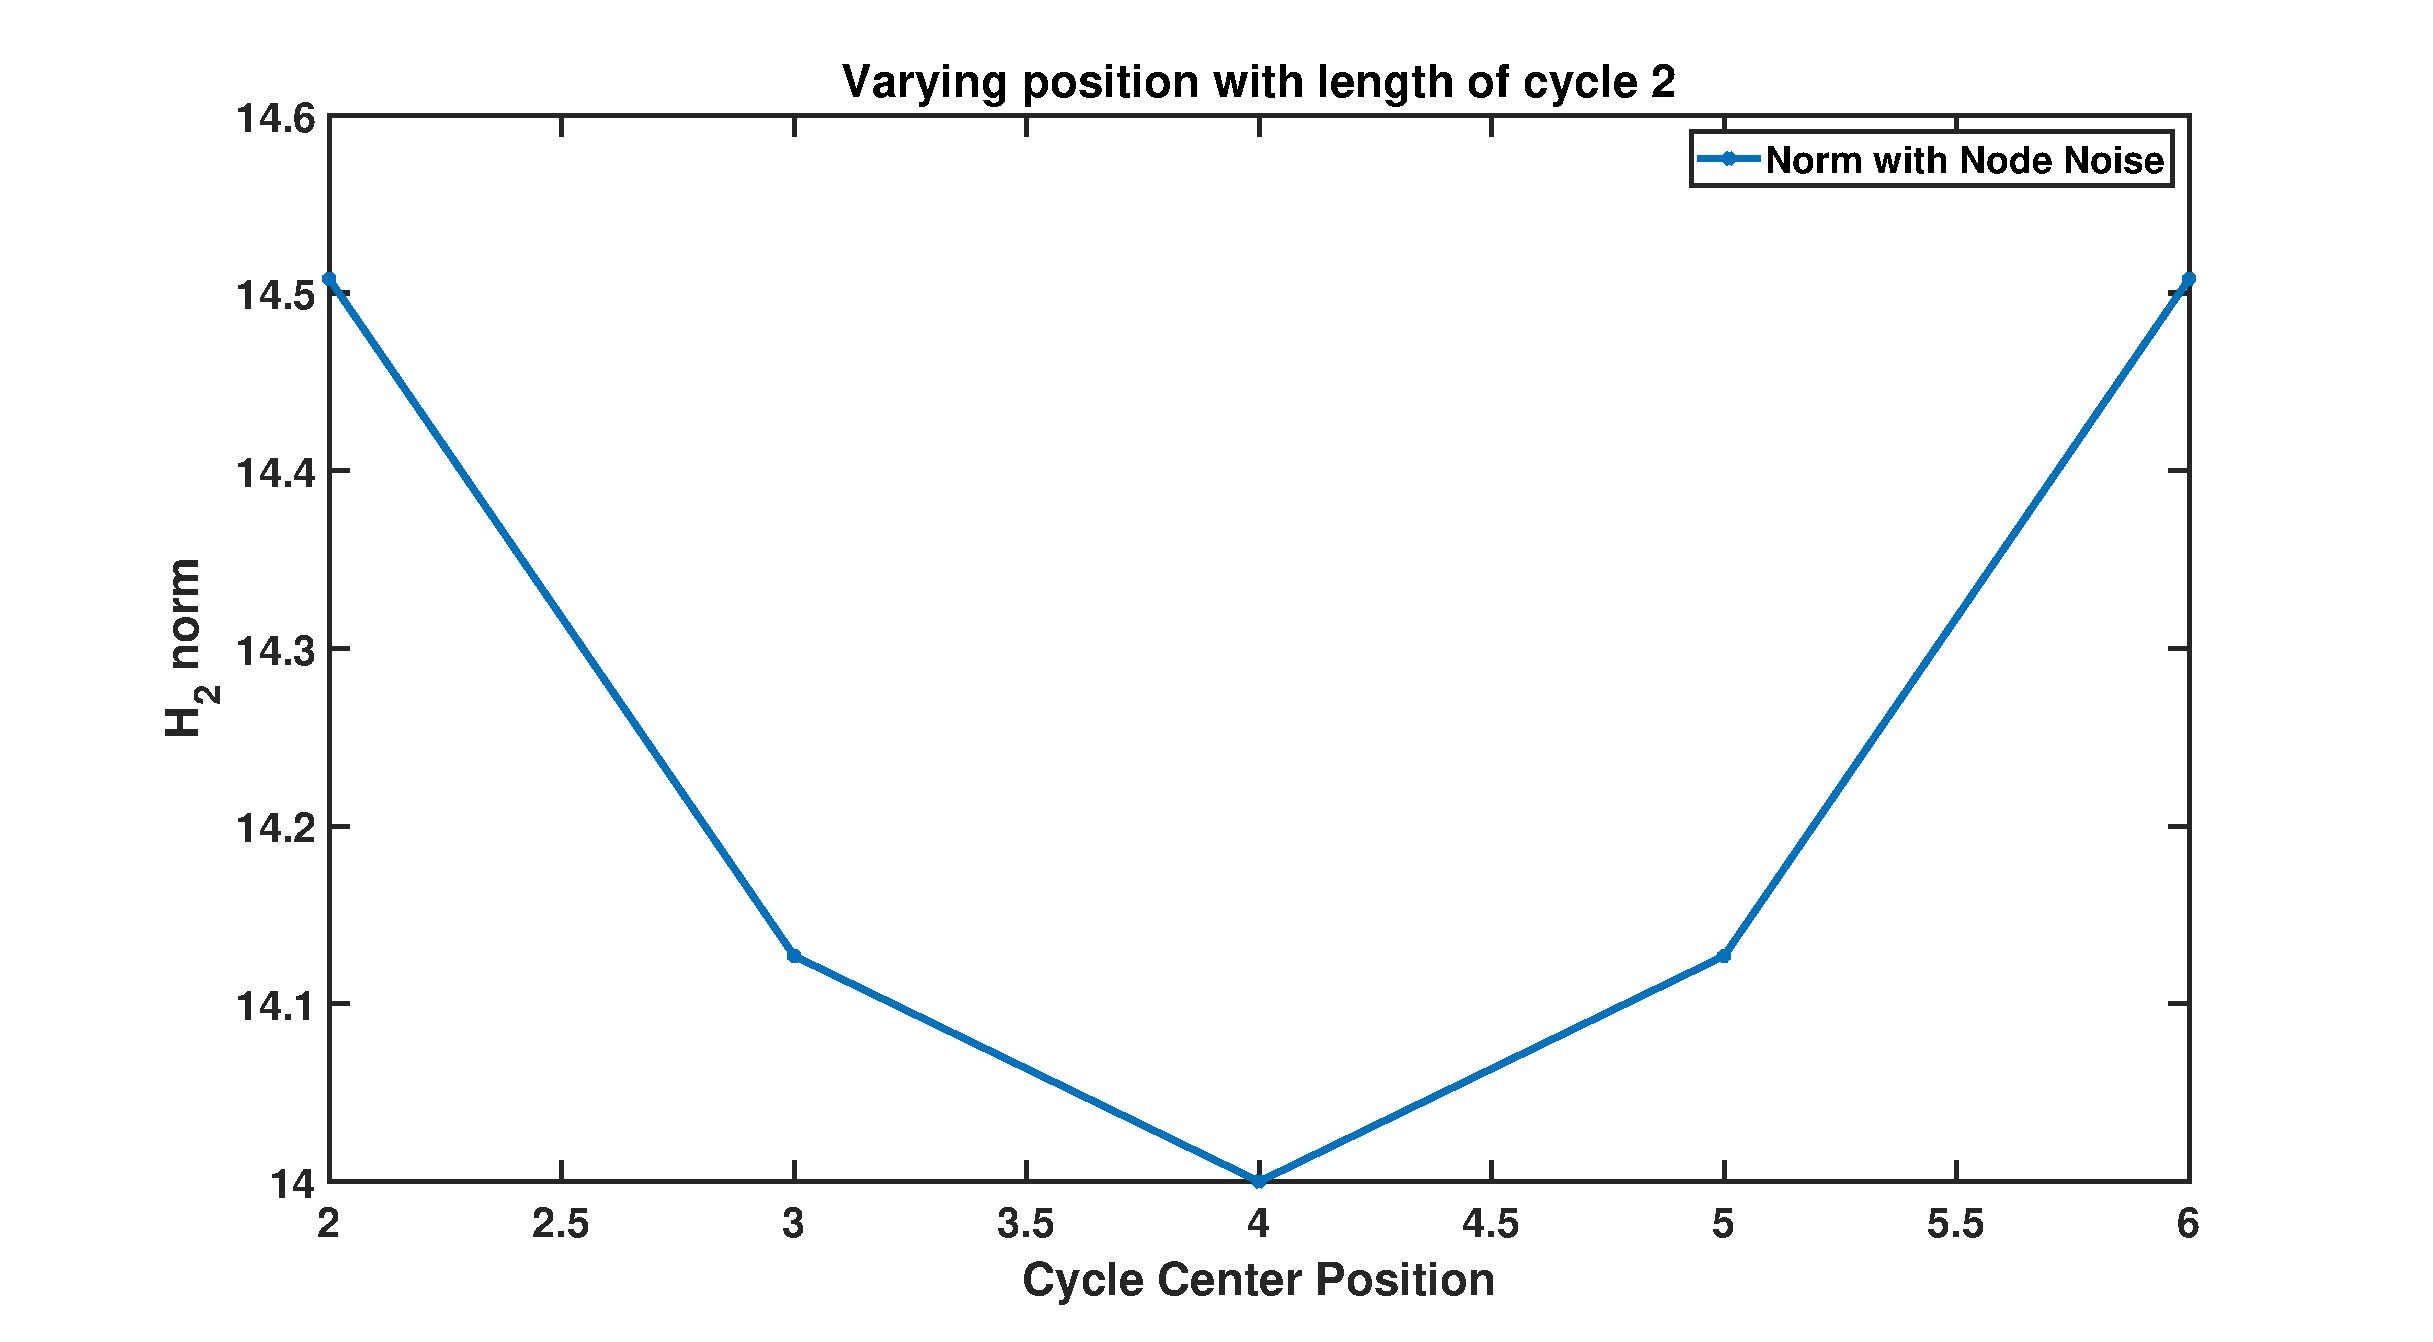
\includegraphics[scale=0.2]{Images/Single_Cycle_Length2_unidrected_Present_Node_Noise.eps}
			\end{figure}
		\end{column}
	\end{columns}
	\vspace{-0.2cm}	
\end{frame}
%%%%%%%%%%%%%%%%%%%%%%%%%%%%%%%%%%%%%%%%%%%%%%%%%%%%

\begin{frame}{Path Graph with Single Cycle}
	\begin{alertblock}{Conclusion}
		\begin{itemize}[]
			\item Performance improves with increase in the value of $\gamma$.
			\item Performance degrades with increase in the network size i.e with increase in $n$.
			\item The performance improves with increase in length of the cycle $\ell$. Hence larger cycles are better. 
			\item If the node noise is zero, then the position of cycle does not impact the performance. Hence, in presence of edge noise only, the size of cycle is enough to characterize the performance. 
			\item However, in presence of node noise with single cycle, the performance depends also on the location of the cycle.
			\item Thus, among two cycles of same size, the cycle towards center of the tree gives better performance. 
		\end{itemize}
	\end{alertblock}
\end{frame}
%%%%%%%%%%%%%%%%%%%%%%%%%%%%%%%%%%%%%%%%%%%%%%%%%%%%
\begin{frame}{Two interacting Cycles in Undirected Path graph}
	\begin{figure}
		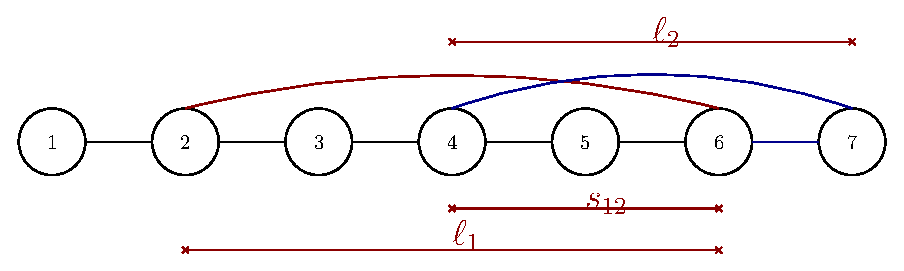
\includegraphics[scale=0.8]{Images/2_InteractingCycles_undirected.eps}
	\end{figure}
	\begin{myblock}{Theorem 4}
		Given an undirected path graph with $n$ node and presence of two cycle of length $\ell_1,\ell_2$ and number of overlapping edges $s_{12}$, then $\mathcal{H}_2$ Norm of System $\Sigma_{\tau}$ is
		
		$$\norm{\Sigma_{\tau}}^2=\frac{1}{2\gamma}\left[\textcolor{violet}{2\sigma_r^2(n-1)}+\textcolor{magenta}{(\sigma_{q}^2+\sigma_r^2)(n-3+D)}+\textcolor{cyan}{\sigma_q^2\text{ trace}[(RR^T)^{-1}\letree^{-1}(RR^T)^{-1}}\right]$$
		
		where $D=\frac{\ell_1+\ell_2+2}{(\ell_1+1)(\ell_2+1)-s_{12}^2}$
		
	\end{myblock}
\end{frame}	
%%%%%%%%%%%%%%%%%%%%%%%%%%%%%%%%%%%%%%%%%%%%%%%%%%%%
\begin{comment}
\begin{frame}{Two interacting Cycles in Undirected Path graph}
	In absence of node noise
	$\norm{\Sigma_{\tau}}^2=\frac{1}{2\gamma}\left[\textcolor{violet}{2\sigma_r^2(n-1)}+\textcolor{magenta}{\sigma_r^2(n-3+D)}\right]$ \\
	Thus, cycle lengths and overlap is enough to characterize performance.
	\begin{figure}
		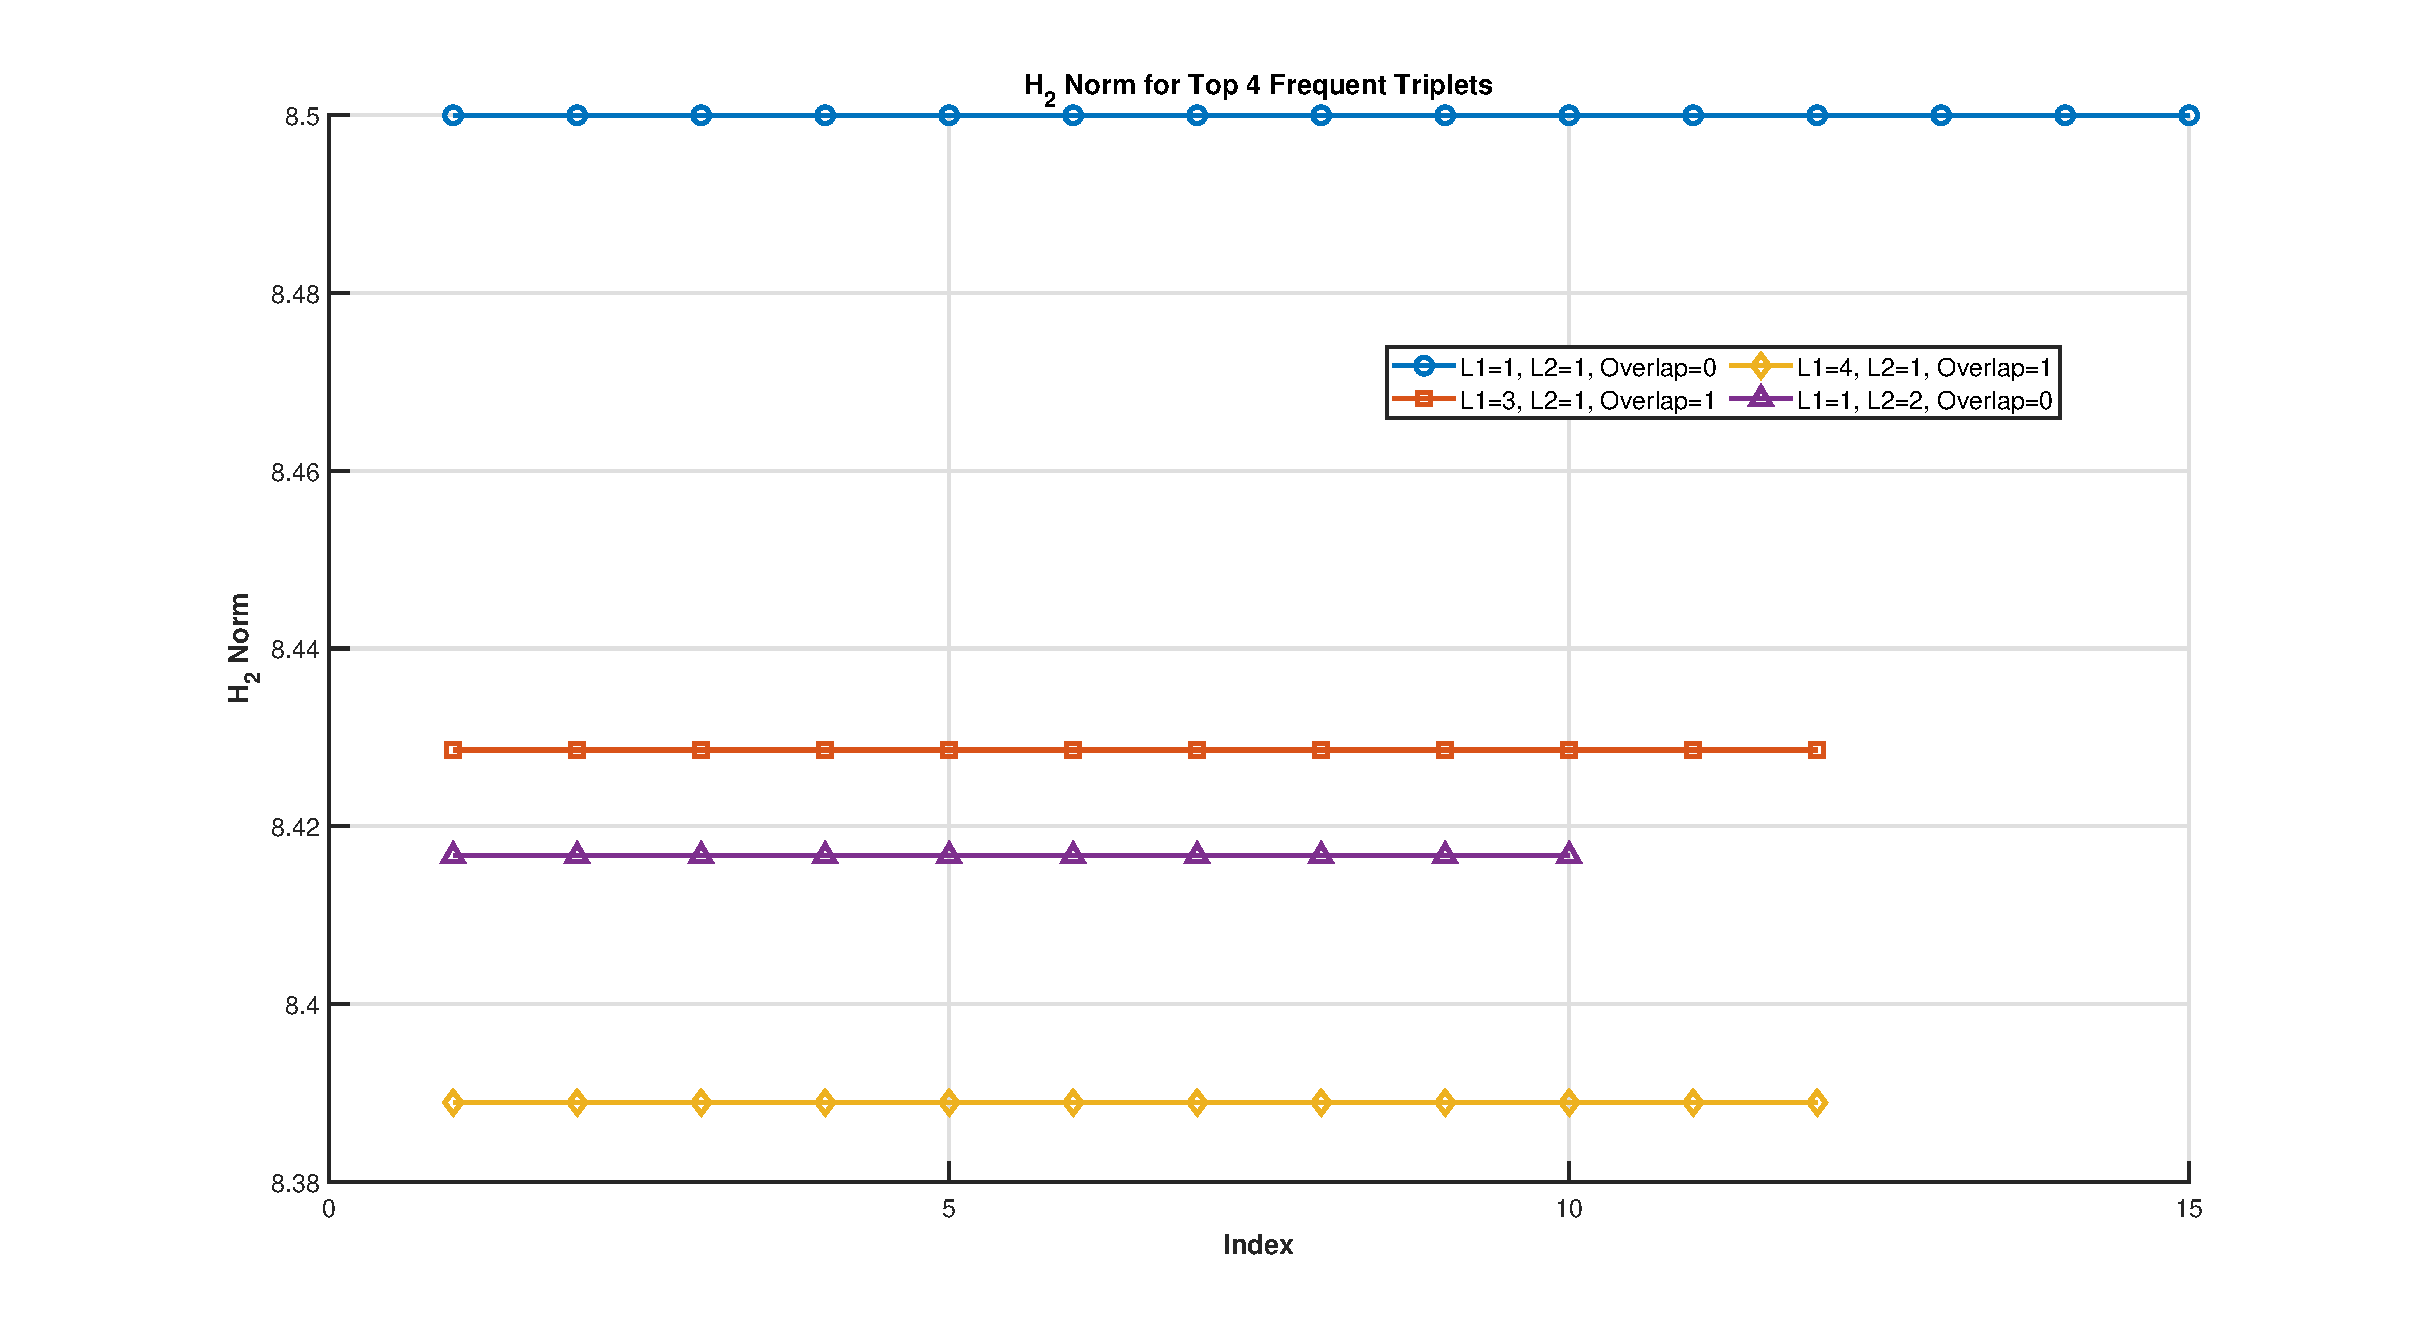
\includegraphics[scale=0.19]{Images/4_most_frequent_triplets.eps}
		\hspace{-0.5cm}
		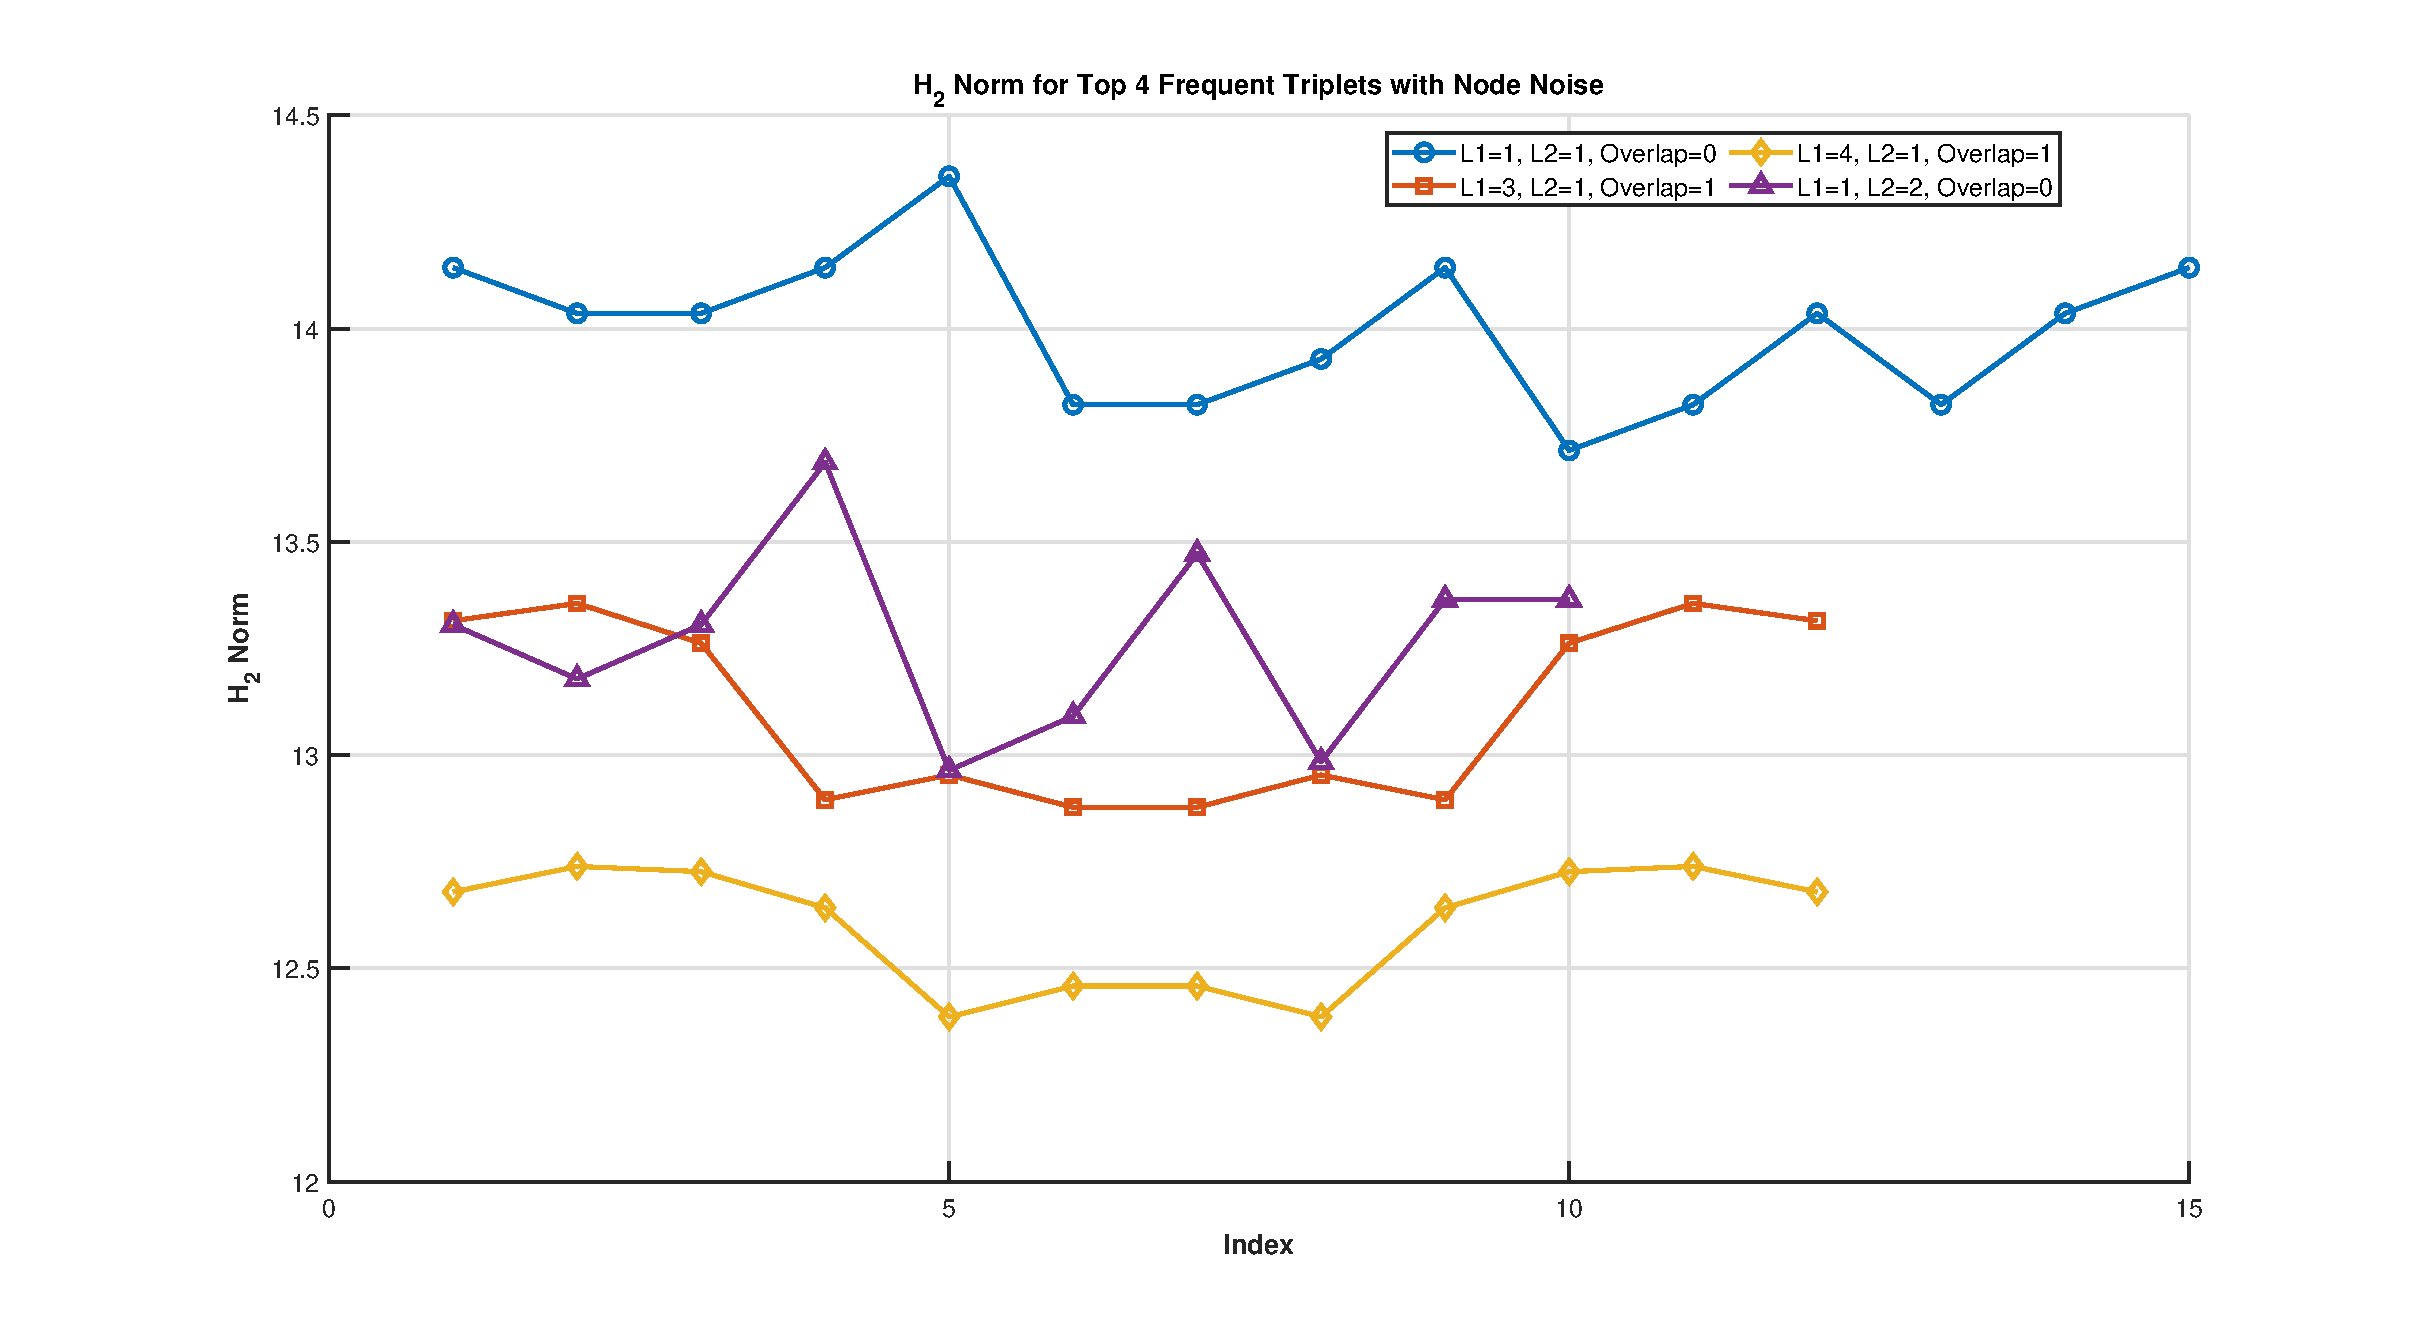
\includegraphics[scale=0.19]{Images/4_most_frequent_triplets_with_node_noise.eps}
	\end{figure}
\end{frame}	
%%%%%%%%%%%%%%%%%%%%%%%%%%%%%%%%%%%%%%%%%%%%%%%%%%%%
\begin{frame}{Two interacting Cycles in Undirected Path graph}
	Lengths Vs $\mathcal{H}_2$ Norm for $n=7$
	\begin{figure}
		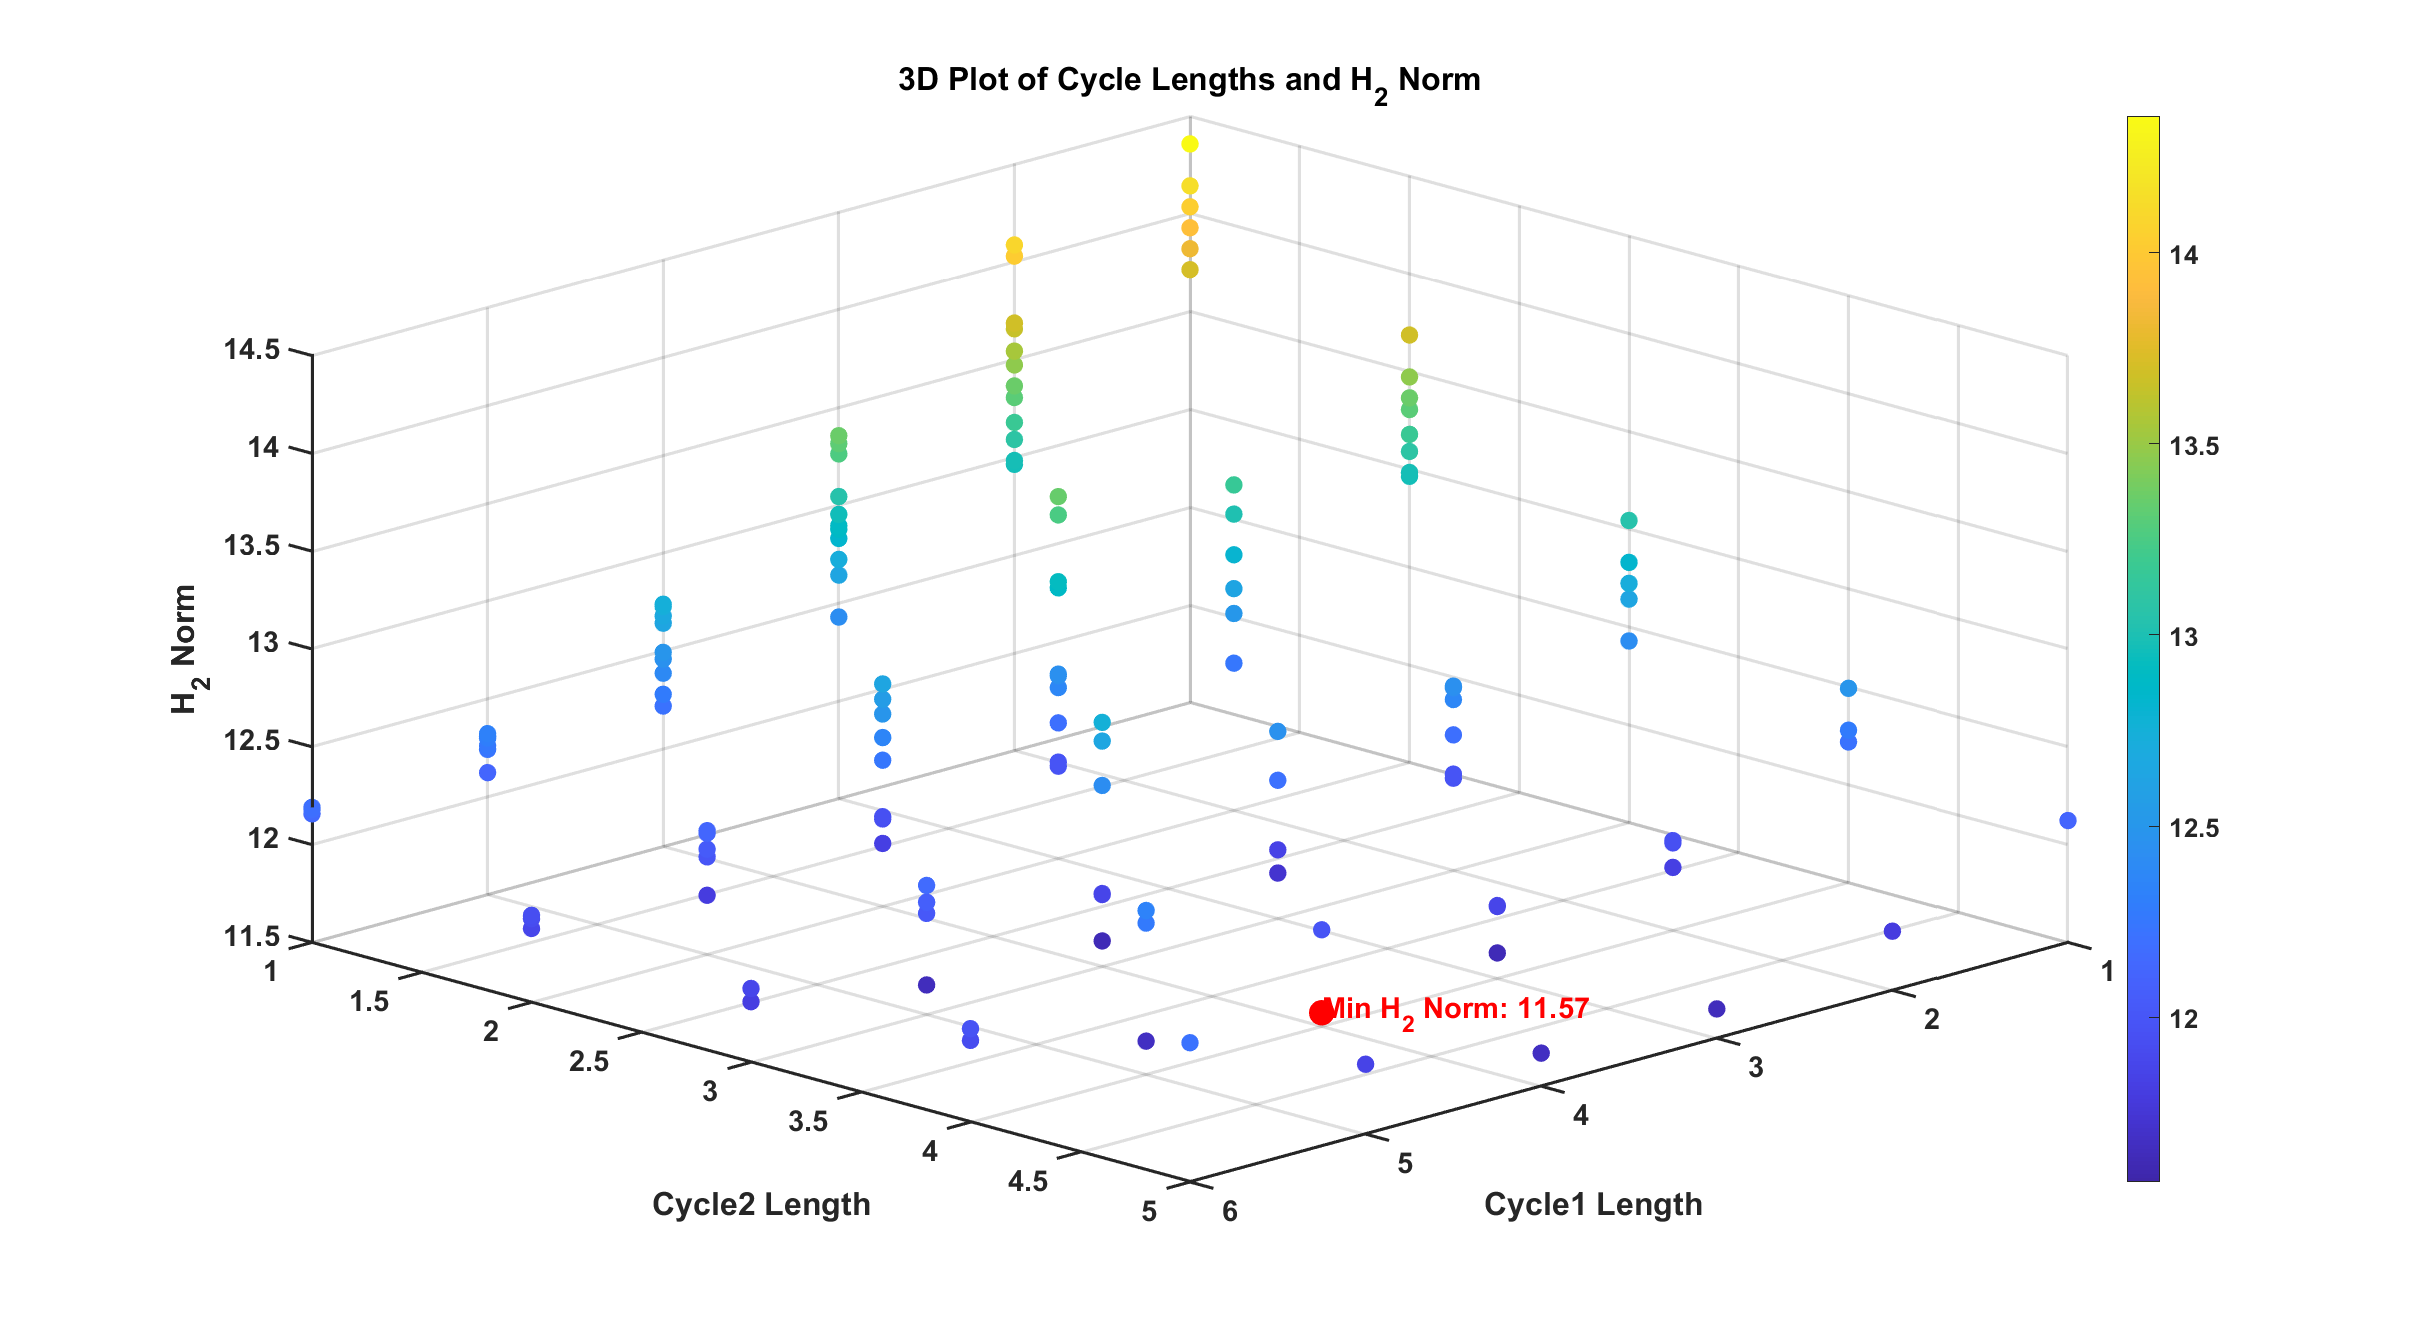
\includegraphics[scale=0.3]{Images/Two_Cycles_Length_Variations_H2_norm.eps}
	\end{figure}
\end{frame}	
%%%%%%%%%%%%%%%%%%%%%%%%%%%%%%%%%%%%%%%%%%%%%%%%%%%%
\begin{frame}{Two interacting Cycles in Undirected Path graph}
	Edge Overlaps Vs $\mathcal{H}_2$ Norm for $n=7$
	\begin{figure}
		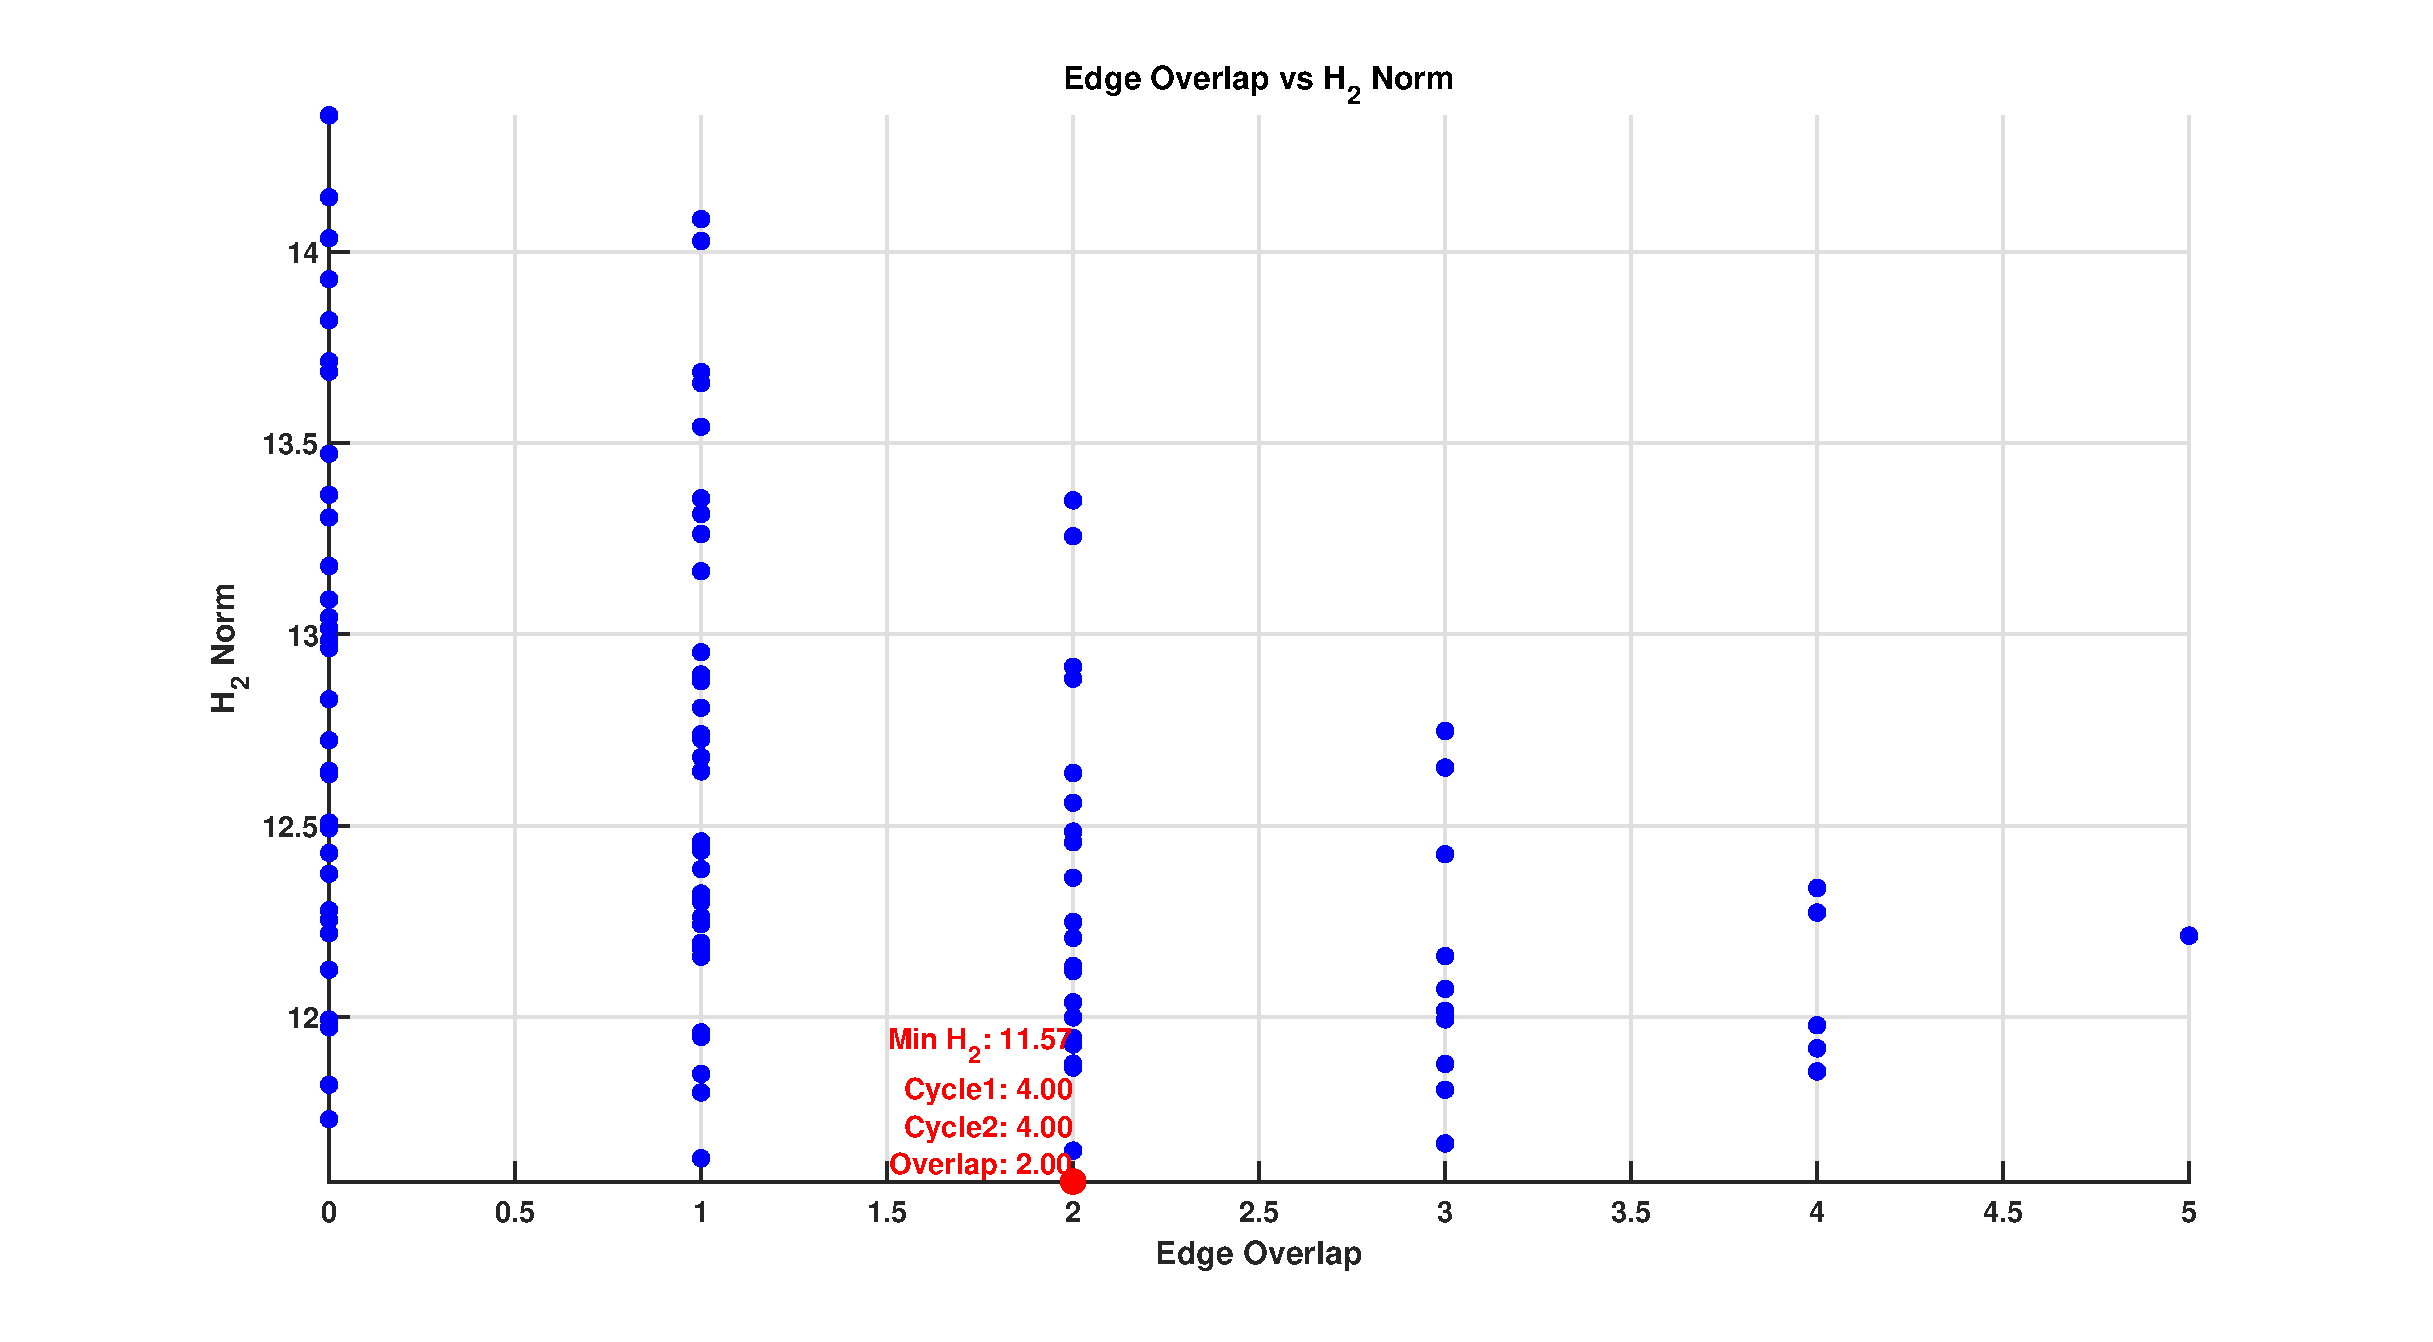
\includegraphics[scale=0.3]{Images/H2_norm_with_edge_overlap.eps}
	\end{figure}
\end{frame}	

\end{comment}
%%%%%%%%%%%%%%%%%%%%%%%%%%%%%%%%%%%%%%%%%%%%%%%%%%%%
\begin{frame}{Path Graph with Two Cycles}
	
	\begin{block}{}
		$\text{Trace}\left[(RR^T)^{-1}\letree^{-1}(RR^T)^{-1}\right]=\text{trace}\left[\letree^{-1}+(\frac{1}{D^2})\letree^{-1}(c_1t_1t_1^T+c_2t_2t_2^T+2c_3t_1t_2^T)\right]$\\
		where, \\
		$t_1,t_2$ are columns of $T$ corresponding to cycles 1 and 2,\\
		$c_1=\ell_1(\ell_2+1)^2-(\ell_2+2)s_{12}^2-2D(\ell_2+1)$\\
		$c_2=\ell_2(\ell_1+1)^2-(\ell_1+2)s_{12}^2-2D(\ell_1+1)$\\
		$c_3=s_{12}(s_{12}^2+2D+1-\ell_1\ell_2)$
		%Given a path graph with $n$ node and two cycle of size $\ell_1, \ell_2$ with $s_{12}$ overlapping edges between the cycles, the $\mathcal{H}_2$ Norm of System $\Sigma_{\tau}$ in presence of node noise depends on the location of cycles and is independent of its location in absence of node noise.
	\end{block}
	\begin{alertblock}{}
	\begin{itemize}
		\item In absence of node noise, the performance only depends on the size of the cycles and the number of overlapping edges but independent of the position of the cycles in the network.
		\item The best performance is achieved with near equal sized cycles ($|\ell_1-\ell_2|\le1$) from two extreme edges of spanning trees.
		\item The number of overlapping edges for best performance increases with the increase in size of network.
	\end{itemize}
\end{alertblock}

\end{frame}
%%%%%%%%%%%%%%%%%%%%%%%%%%%%%%%%%%%%%%%%%%%%%%%%%%%%
\begin{comment}
\begin{frame}{For Directed Path Graph}
	\begin{figure}
		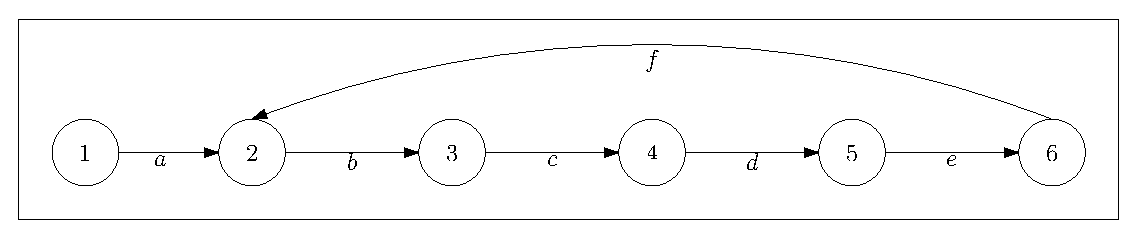
\includegraphics[scale=0.4]{Images/example_network.eps}		\\
	\end{figure}
	\vspace{-0.3cm}
\begin{defi}[In-incidence Matrix{\footnotemark[1]}]
				The In-incidence matrix for a digraph $\mathcal{G}$ is defined such that $E_{in}(\mathcal{G})_{ij}=-1$ if edge $e_j$ is incoming at vertex $i$ and $E(\mathcal{G})_{ij}=0$ otherwise.
\end{defi}
$E_{in}=\begin{bsmallmatrix}
				0 &  0 &  0 &  0 &  0 & \color{cyan}{0} \\
				-1 &  0 &  0 &  0 &  0 & \color{cyan}{-1} \\
				0 & -1 &  0 &  0 &  0 & \color{cyan}{0} \\
				0 &  0 & -1 &  0 &  0 & \color{cyan}{0} \\
				0 &  0 &  0 & -1 &  0 & \color{cyan}{0} \\
				0 &  0 &  0 &  0 & -1 & \color{cyan}{0} \\
\end{bsmallmatrix}$;
			$~~E_{in}=\begin{bmatrix}\etreein & \color{cyan}{E_{c_{in}}}\end{bmatrix}=\etreein \begin{bmatrix} I_{n-1} & \color{cyan}{\tilde{T}}\end{bmatrix}=\etreein \tilde{R}$,\\
			where $\tilde{T}=\begin{bmatrix}1 & 0 & 0 & 0 & 0 \end{bmatrix}^T=(\etreein^T\etreein)^{-1}\etreein^TE_{c_{in}}$\\
\textcolor{red}{Note:} Relation above holds only if graph has a \color{blue}{unique root node}.
	\footnotetext[1]{Mukherjee, Dwaipayan, and Daniel Zelazo. "Robustness of consensus over weighted digraphs." IEEE Transactions on Network Science and Engineering 6.4 (2018): 657-670.}
\end{frame}

%%%%%%%%%%%%%%%%%%%%%%%%%%%%%%%%%%%%%%%%%%%%%%%%%%%%
\begin{frame}
	\begin{block}{Reduced Order Edge Dynamics}
		Applying similar coordinate transformation to separate the zero eigenvalue, the reduced order system ($\Sigma_{\tau}$) can be represented as:
		$$\dot{X}_{e_\tau}=\begin{bmatrix}
			\mathbf{0} & I_{n-1}\\
			-\letreein \tilde{R}R^T & -\gamma\letreein \tilde{R}R^T
		\end{bmatrix}X_{e_\tau}+\begin{bmatrix}
			\mathbf{0} & \mathbf{0}\\
			\sigma_{q}E^T & -\sigma_{r}\letreein \tilde{R}
		\end{bmatrix}\hat{N}(t)$$
		$$z(t)=X_{e_\tau}$$
		where, ${X}_{e_\tau} \in \R^{2(n-1)},~ \hat{N}(t) \in \R^{(n+|e|)} $ is the normalized noise signal.
	\end{block}
	\pause
	\begin{block}{$\mathcal{H}_2$ norm}
		The $\mathcal{H}_2$ Norm of the system $\Sigma_{\tau}$, where, $A=\begin{bmatrix}
			\mathbf{0} & I_{n-1}\\
			-\letreein \tilde{R}R^T & -\gamma\letreein \tilde{R}R^T
		\end{bmatrix}$, $B=\begin{bmatrix}
			\mathbf{0} & \mathbf{0}\\
			\sigma_{q}E^T & -\sigma_{r}\letreein \tilde{R}
		\end{bmatrix}$ and $C=I_{n-1}$ is given by $$\norm{\Sigma_{\tau}}_2^2=trace(P)$$
		where $P$ is the solution to the Lyapunov equation $AP+PA^T+BB^T=0,$
	\end{block}							
\end{frame}


\begin{frame}{$\mathcal{H}_2$ Norm of the system with variation in $\gamma$ }
	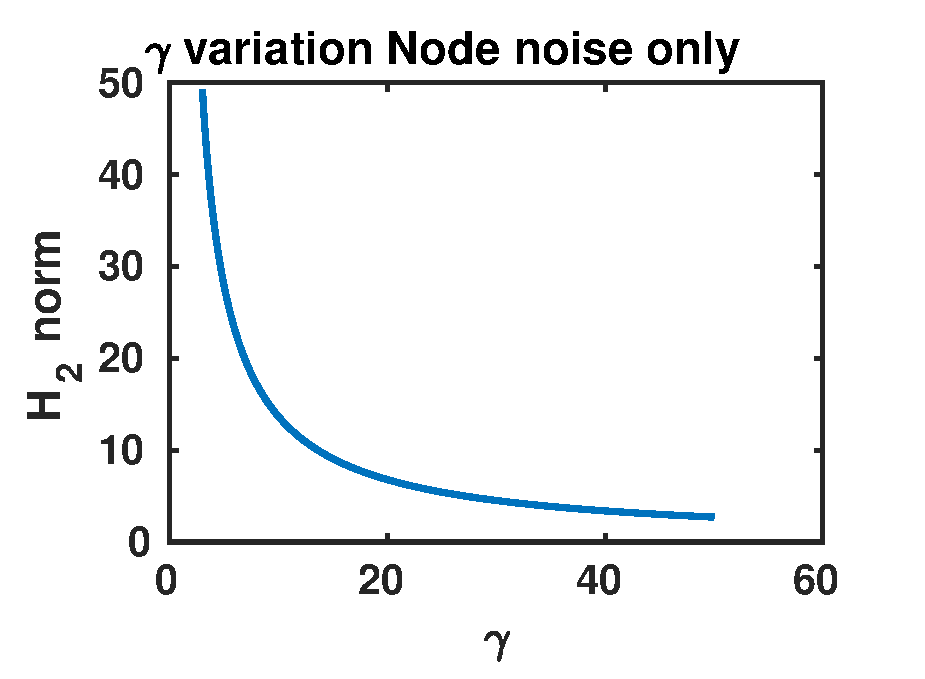
\includegraphics[scale=0.33]{Images/H2normwithgamma_Nodenoise.eps}
	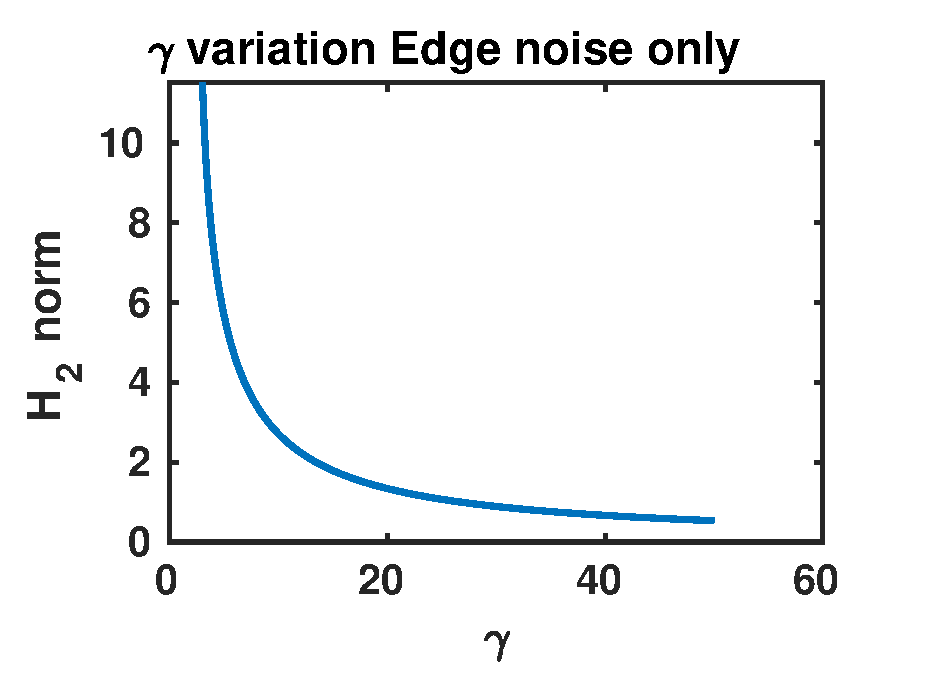
\includegraphics[scale=0.33]{Images/H2normwithgamma_Edgenoise.eps}
	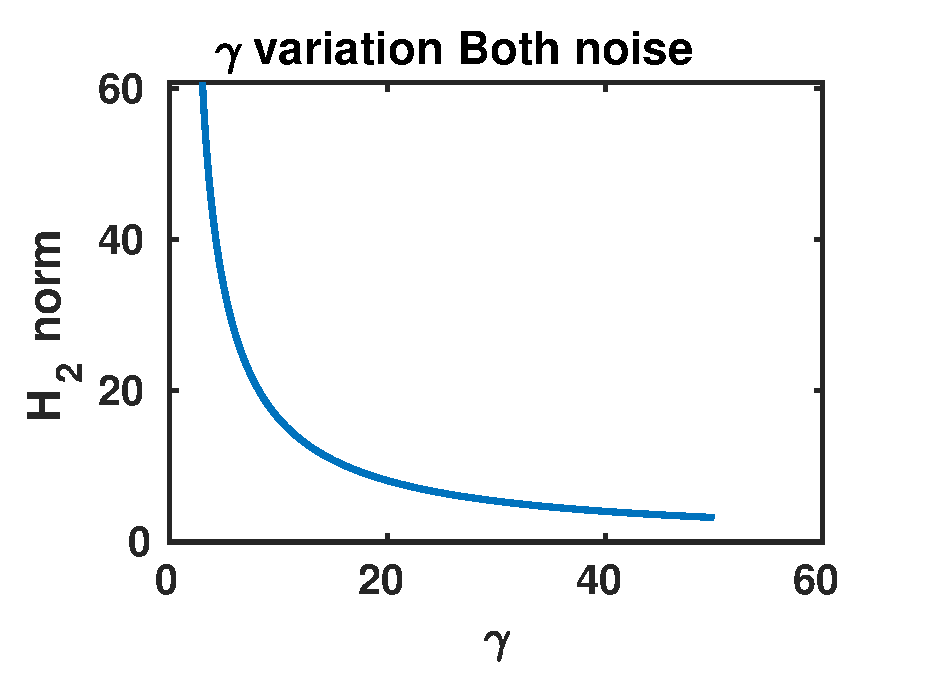
\includegraphics[scale=0.33]{Images/H2normwithgamma_Bothnoise.eps}\\
	\centering
	$\color{blue}J=2\gamma\left[2\gamma^2(I_{n-1} \otimes A_3+A_3 \otimes I_{n-1})+2I_{(n-1)^2}-(A_3^{-1} \otimes A_3+A_3 \otimes A_3^{-1})\right]^{-1}$\\
	$\color{magenta}\text{vec}(P_3)=J\text{vec}(-QQ^T)$\\
	%	\vspace{-0.4cm}
	$\color{magenta}\text{vec}(P_1)=(-1/2)(I_{n-1}\otimes A_3^{-1}+A_3^{-1} \otimes I_{n-1})\text{vec}(P_3)$\\
	$\mathcal{H}_2$ norm of the system $\color{cyan}\norm{\Sigma{\tau}}_2^2=trace(P)=trace(P_1)+trace(P_3)$\\
	\begin{block}{}
		-- The influence of $\gamma$ is encapsulated solely by $J$, and it has an inverse impact on the $\mathcal{H}_2$ performance.\\
		-- Larger values of $\gamma$ not only facilitate consensus but also help in mitigating the effects of noise.
	\end{block}
\end{frame}
%%%%%%%%%%%%%%%%%%%%%%%%%%%%%%%%%%%%%%%%%%%%%%%%%%%%
\begin{frame}{$\mathcal{H}_2$ Norm of the system with cycle length in presence of single cycle}
\begin{figure}
	\centering
	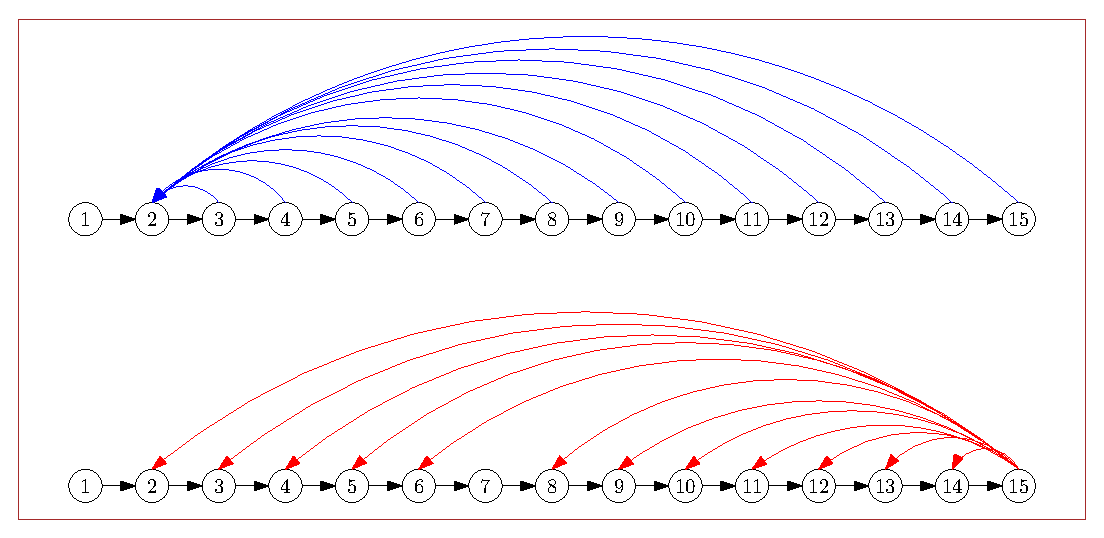
\includegraphics[scale=0.35]{Images/cycle_length.eps}
\end{figure}
\vspace{-0.5cm}
\begin{columns}
	\begin{column}{0.5\textwidth}
		%\vspace{-0.1cm}
		\begin{figure}
			%\hspace{-1cm}
			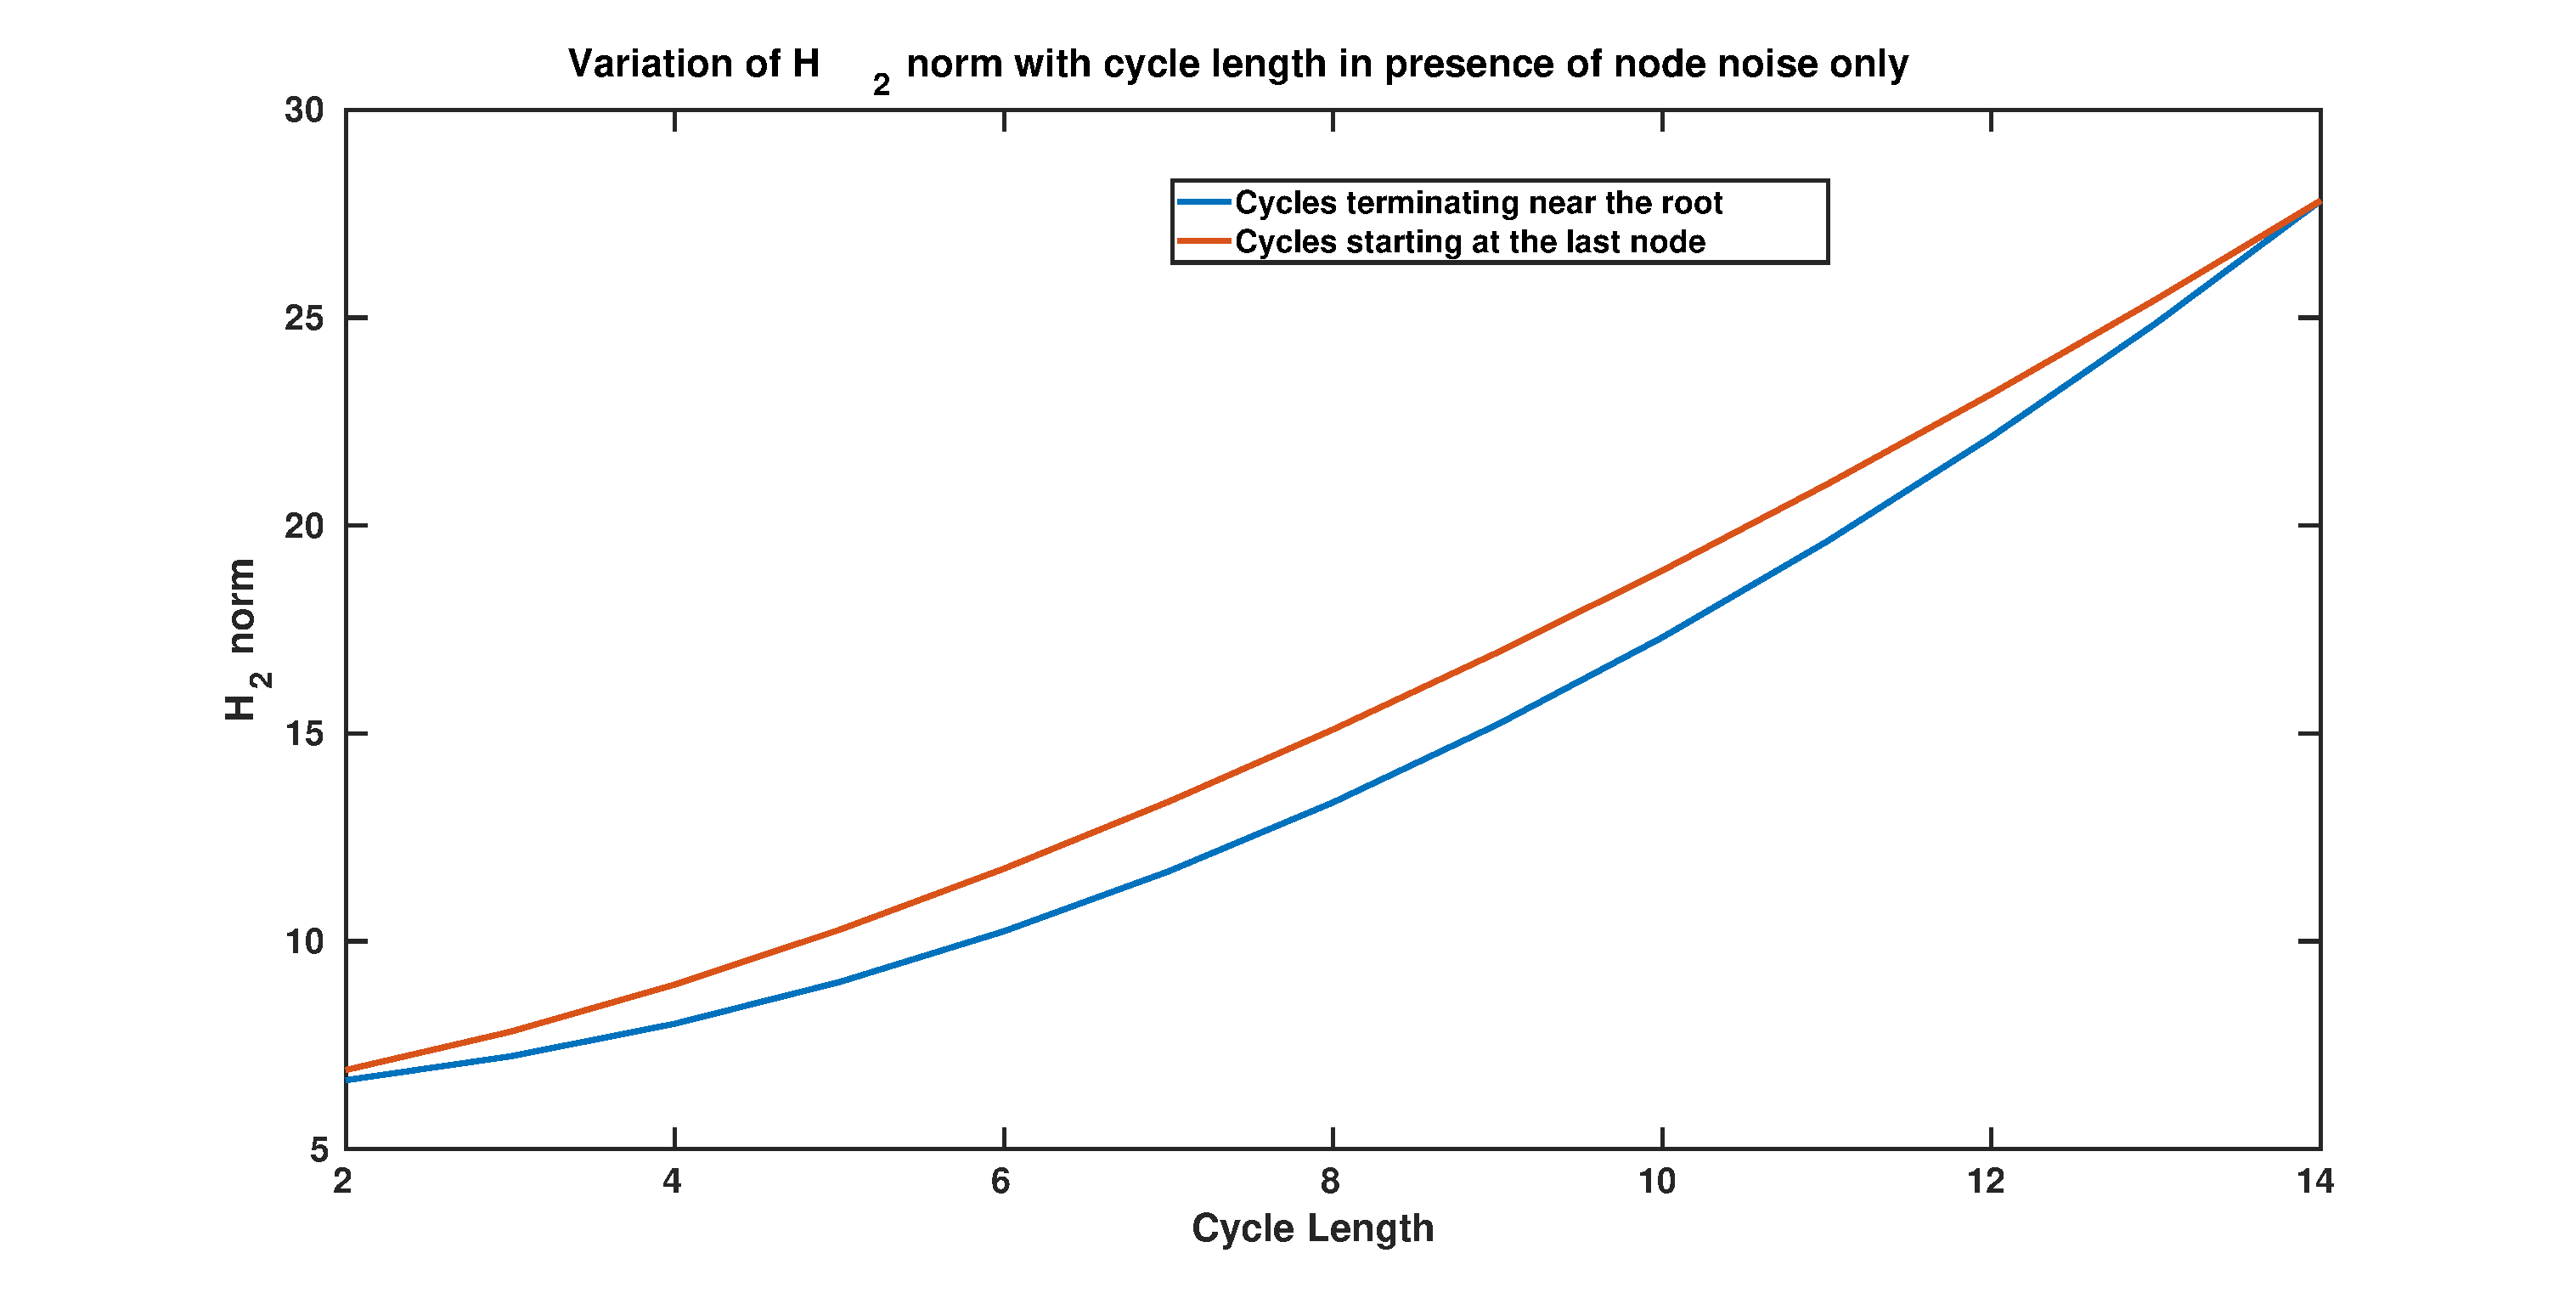
\includegraphics[scale=0.15]{Images/H2normwithcyclelength_Nodenoise.eps}
		\end{figure}
		\vspace{-0.7cm}
	\end{column}
	\begin{column}{0.5\textwidth}
		\vspace{0.5cm}
		\begin{figure}
			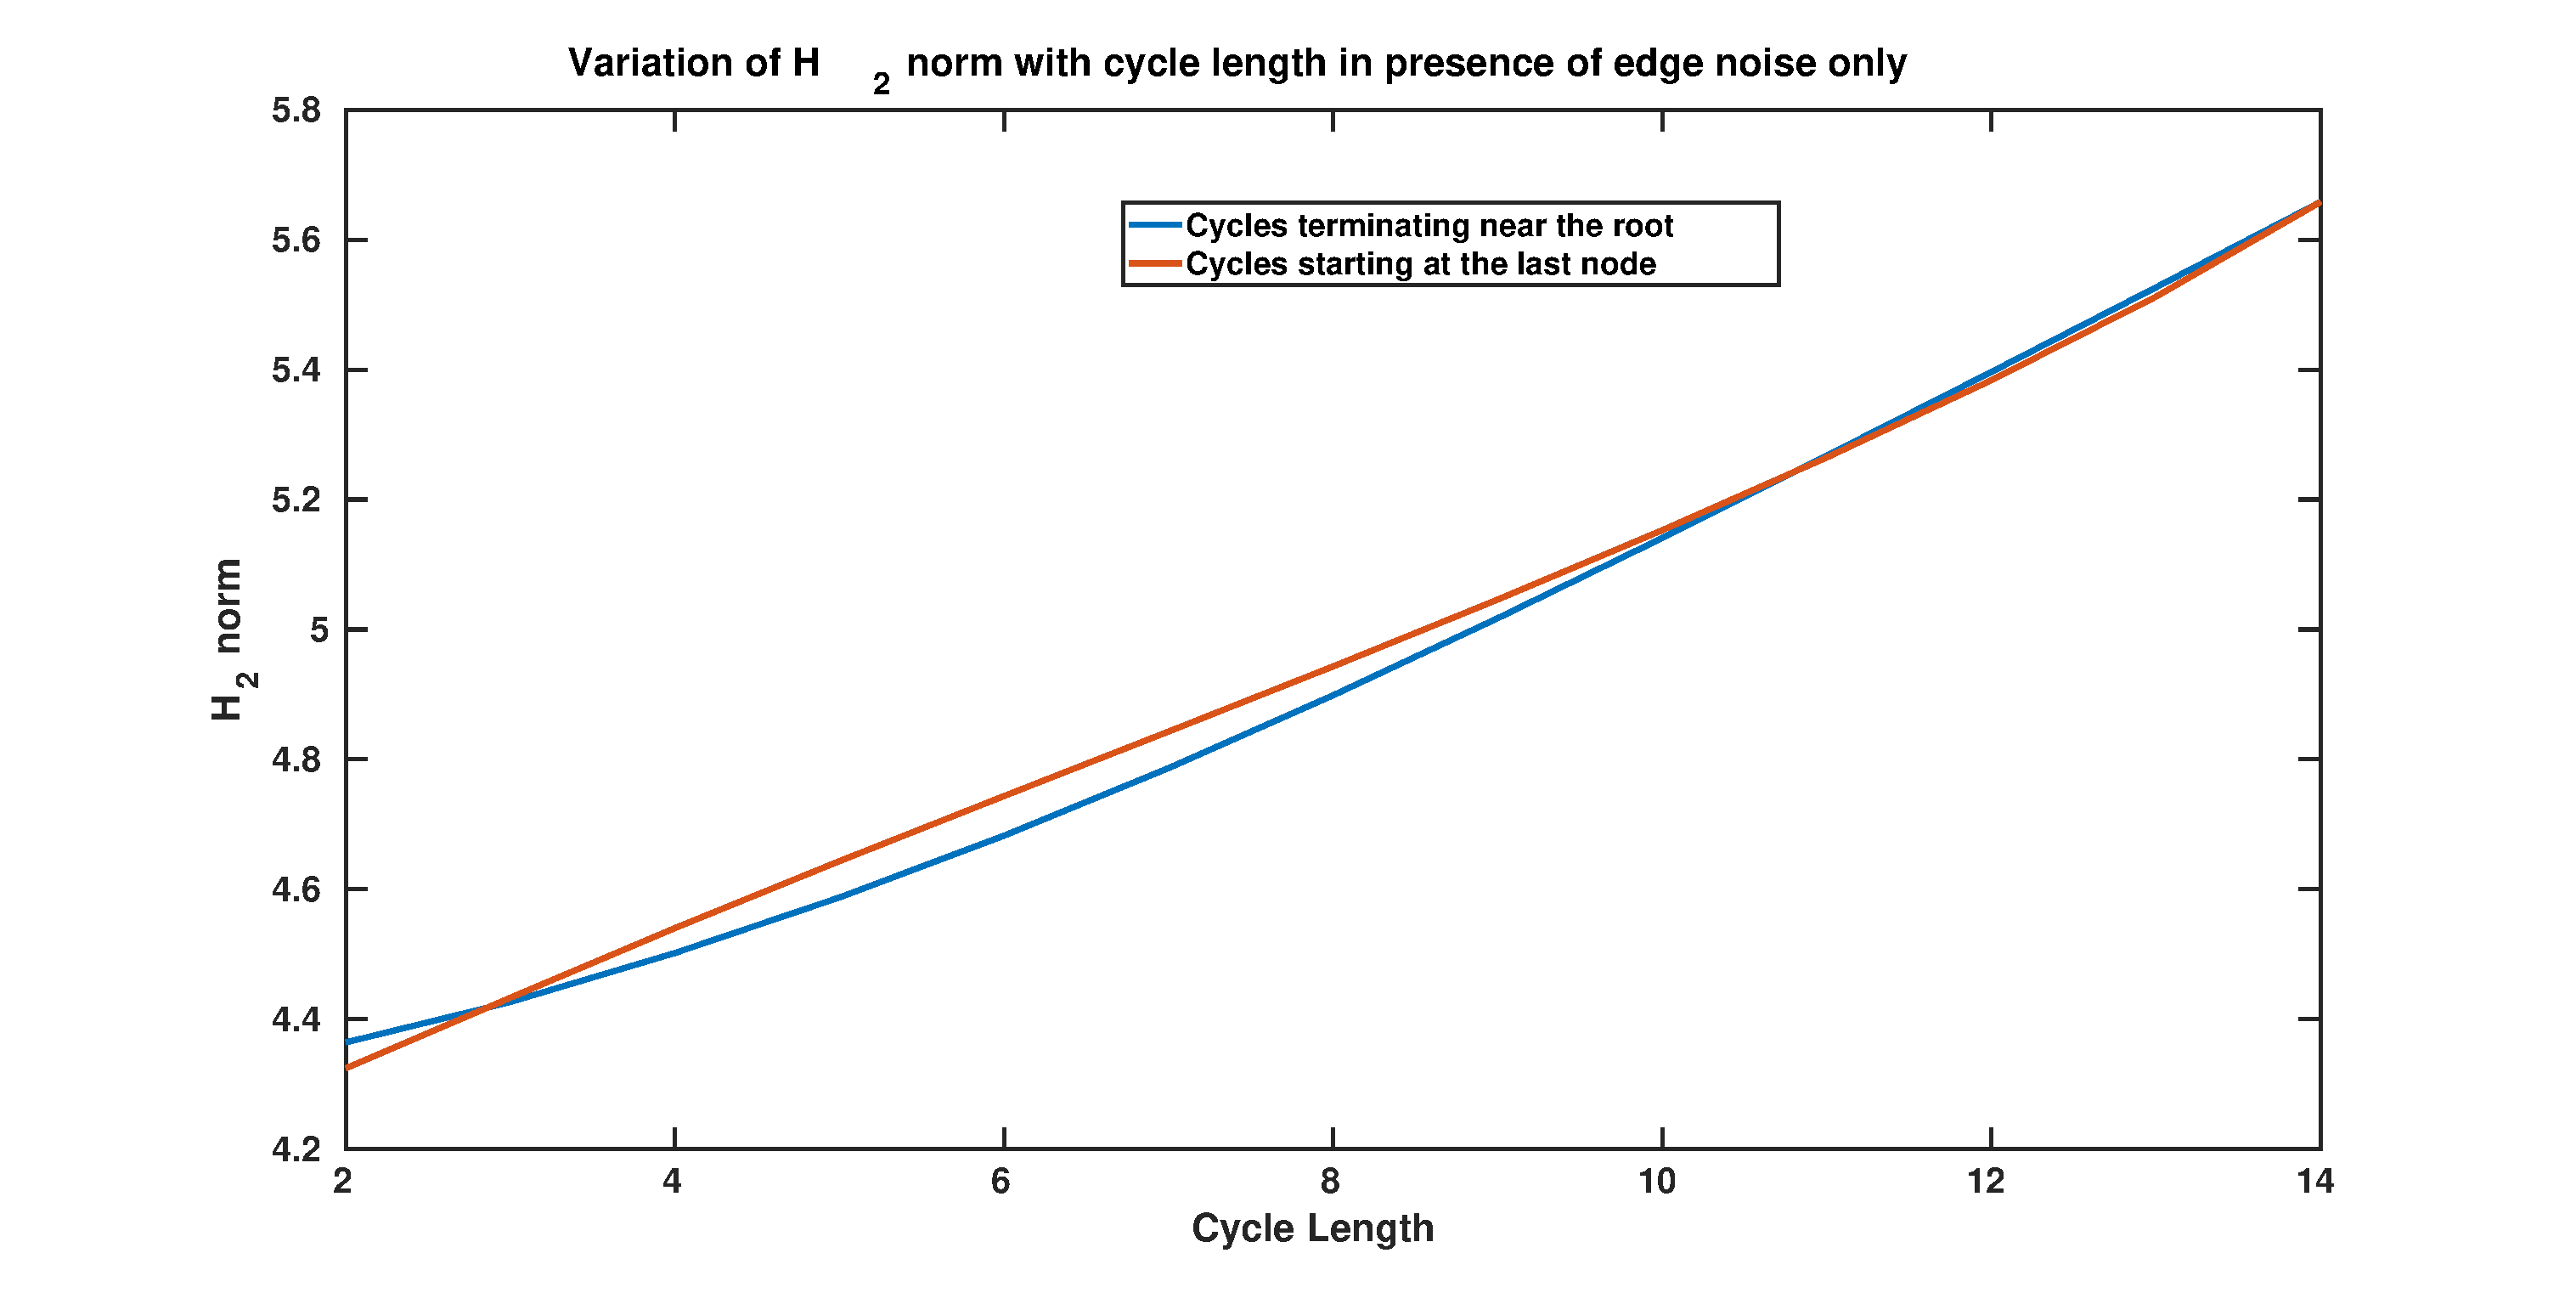
\includegraphics[scale=0.15]{Images/H2normwithcyclelength_Edgenoise.eps}
		\end{figure}
	\end{column}
\end{columns}
\vspace{-0.2cm}
\end{frame}
%%%%%%%%%%%%%%%%%%%%%%%%%%%%%%%%%%%%%%%%%%%%%%%%%%%%
\begin{frame}{$\mathcal{H}_2$ Norm of the system with cycle length in presence of single cycle}
	\begin{figure}
	\centering
	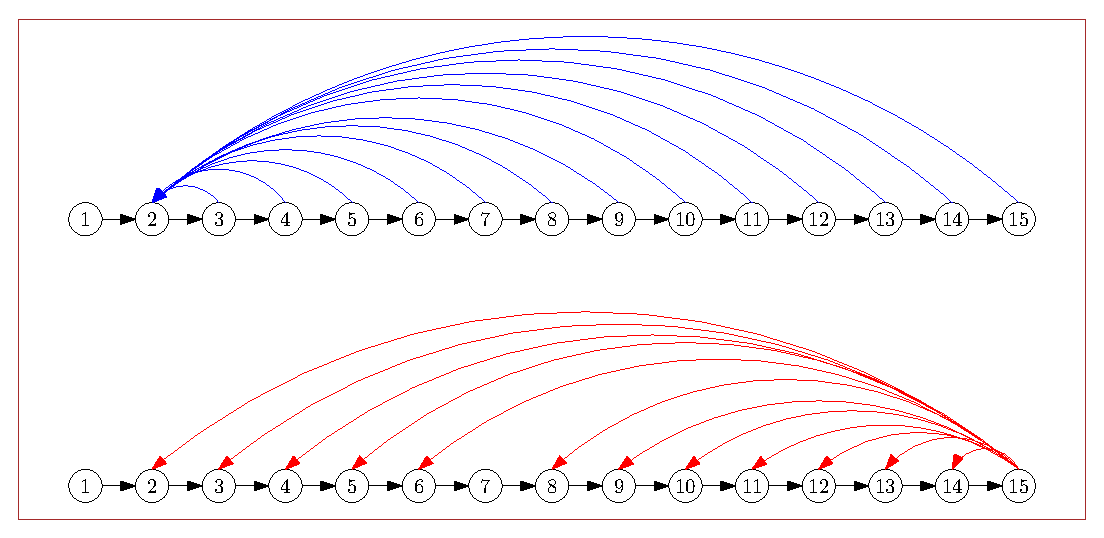
\includegraphics[scale=0.35]{Images/cycle_length.eps}
\end{figure}
\vspace{-0.5cm}
	\begin{columns}
		\begin{column}{0.5\textwidth}
			\begin{figure}
				\centering
				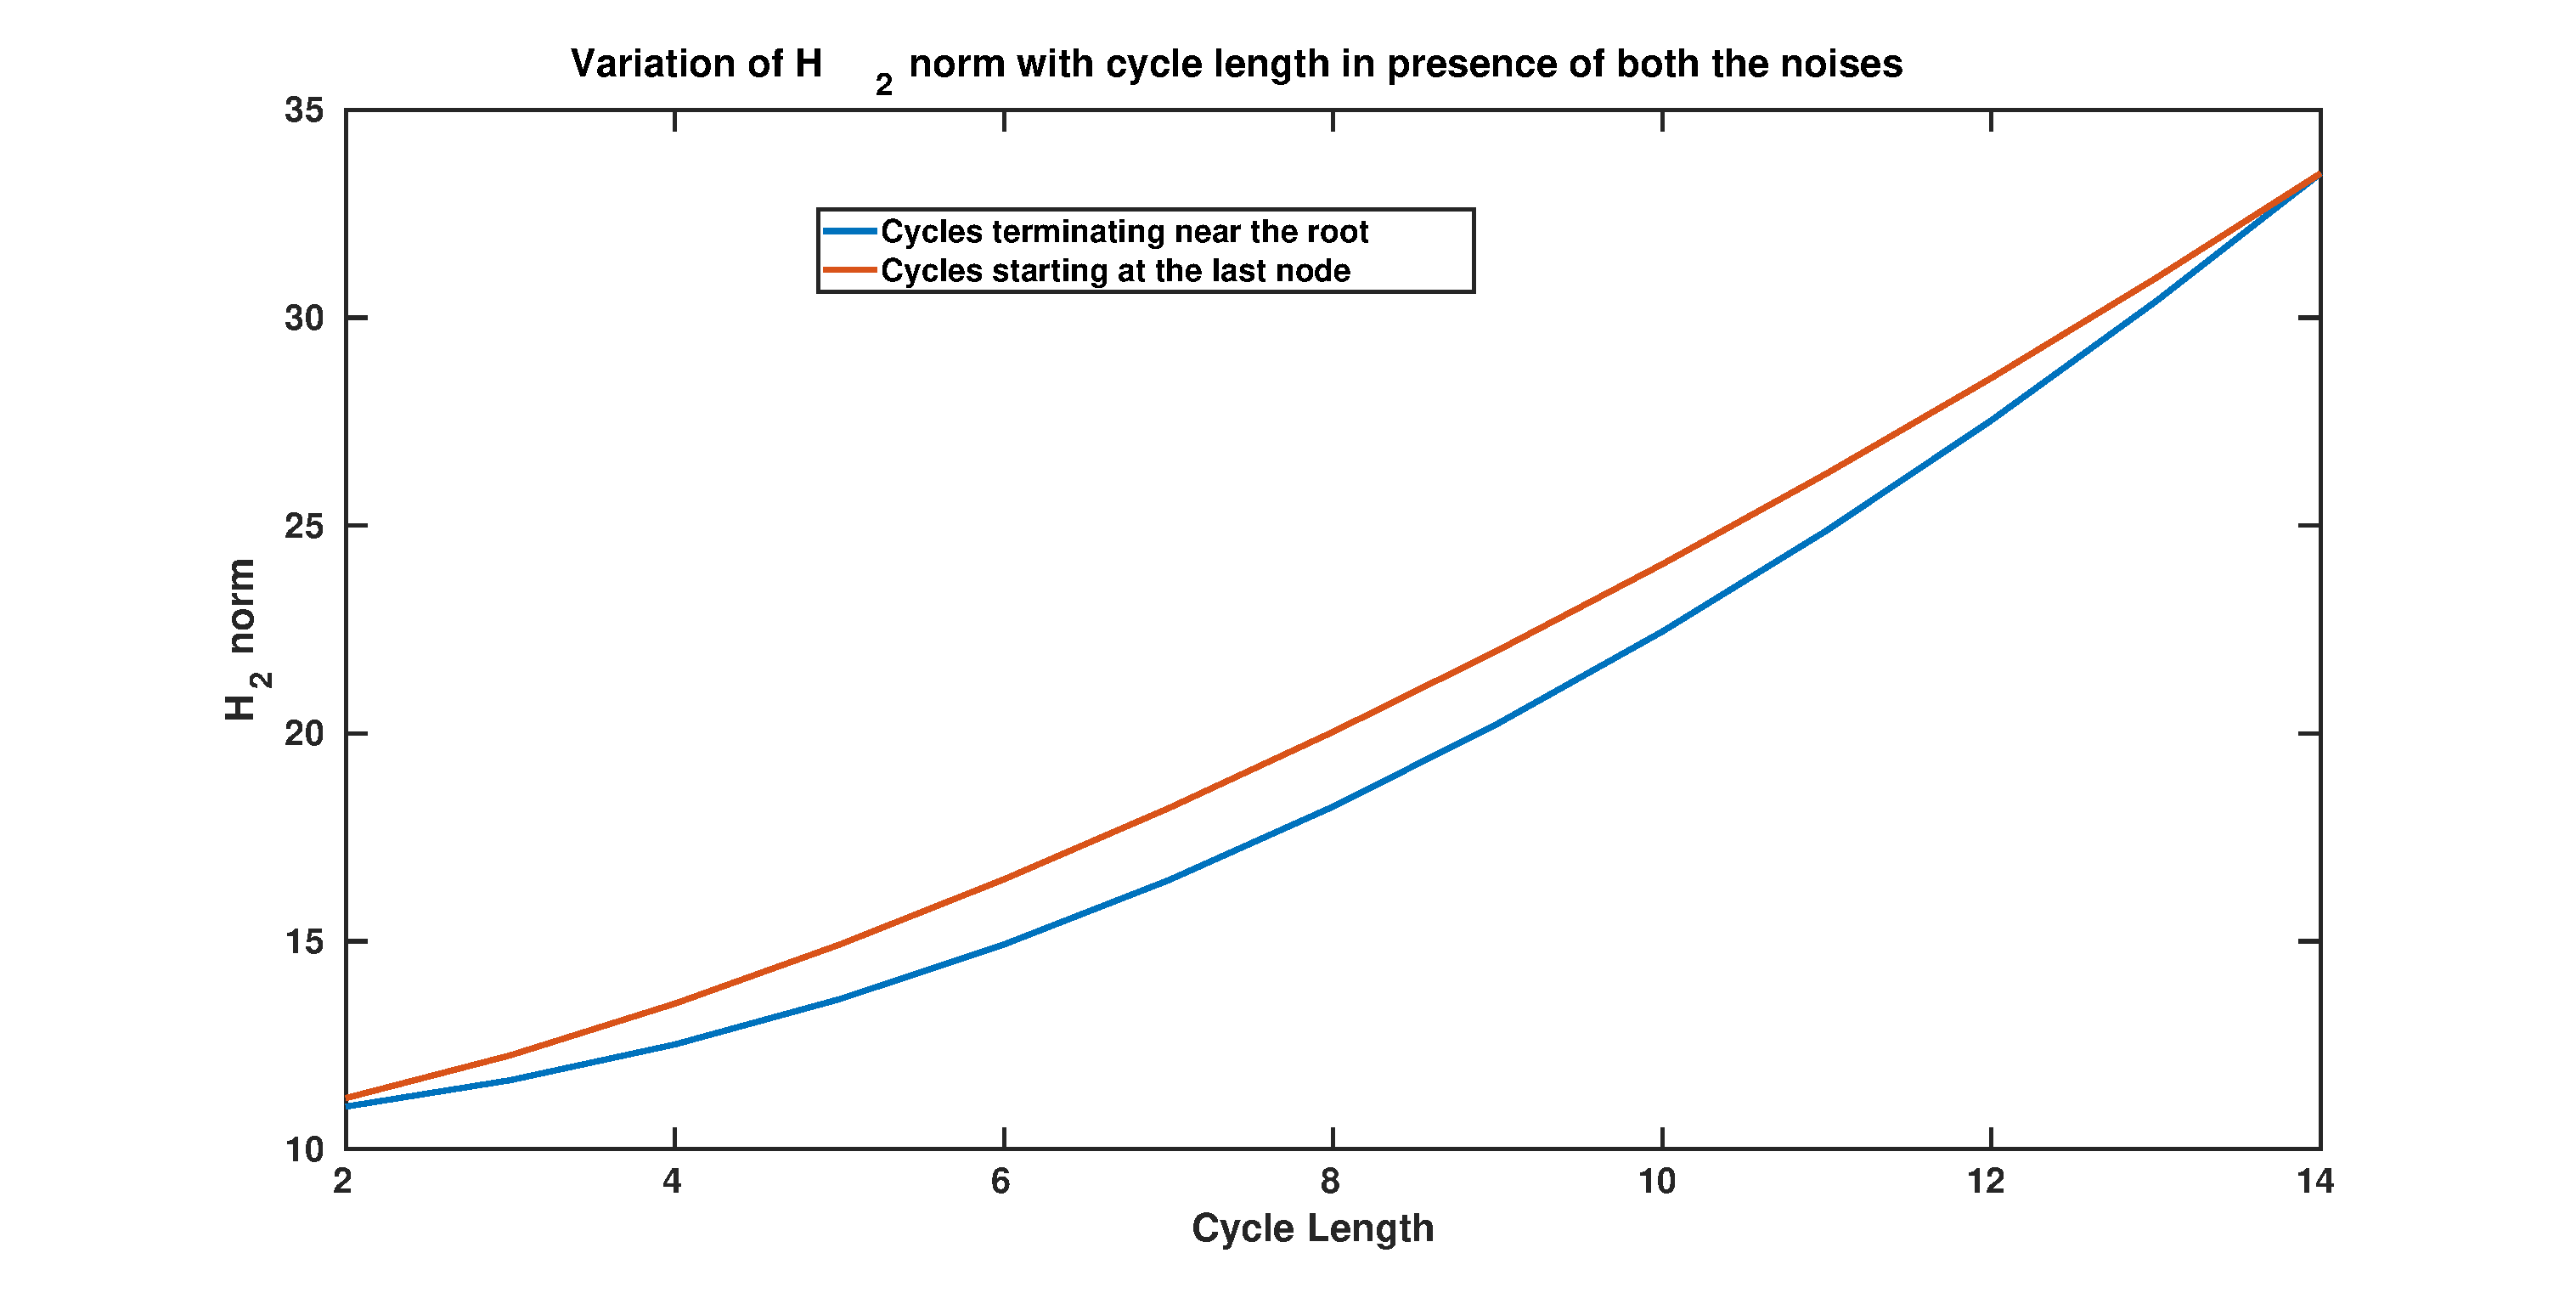
\includegraphics[scale=0.15]{Images/H2normwithcyclelength_Bothnoise.eps}
			\end{figure}
		\end{column}
		\begin{column}{0.5\textwidth}
			\begin{itemize}
				\item Cycles closer to root nodes are better.
				\item Smaller Cycles are better.
				\item Node Noise dominates the performance.
			\end{itemize} 
		\end{column}
	\end{columns}
	\vspace{-0.2cm}
\end{frame}
%%%%%%%%%%%%%%%%%%%%%%%%%%%%%%%%%%%%%%%%%%%%%%%%%%%%
\begin{frame}{$\mathcal{H}_2$ Norm of the system with varying position and cycle length}
	%\vspace{-1cm}
	\begin{columns}
		\begin{column}{0.6\textwidth}
			\vspace{-0.5cm}
			\begin{figure}
				%\hspace{-1cm}
				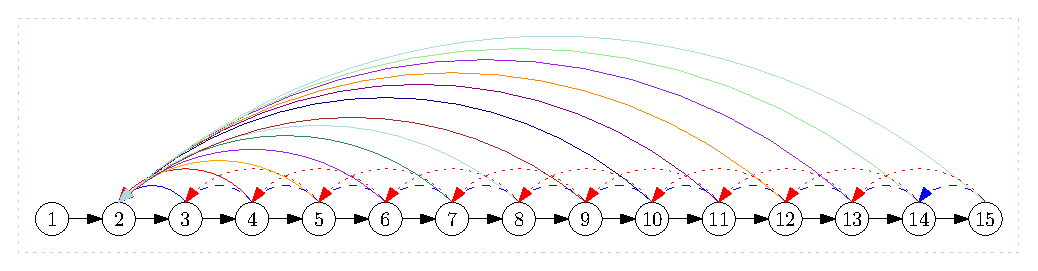
\includegraphics[scale=0.45]{Images/cycle_position_length.eps}
			\end{figure}
		\end{column}
		\begin{column}{0.5\textwidth}
			\vspace{-0.5cm}
			\begin{itemize}
				\item Performance changes with cycle position.
				\item Node Noise and Edge noise, both have positional dependence.
			\end{itemize}	
		\end{column}
	\end{columns}
	\begin{columns}
	\begin{column}{0.3\textwidth}
		\begin{figure}
			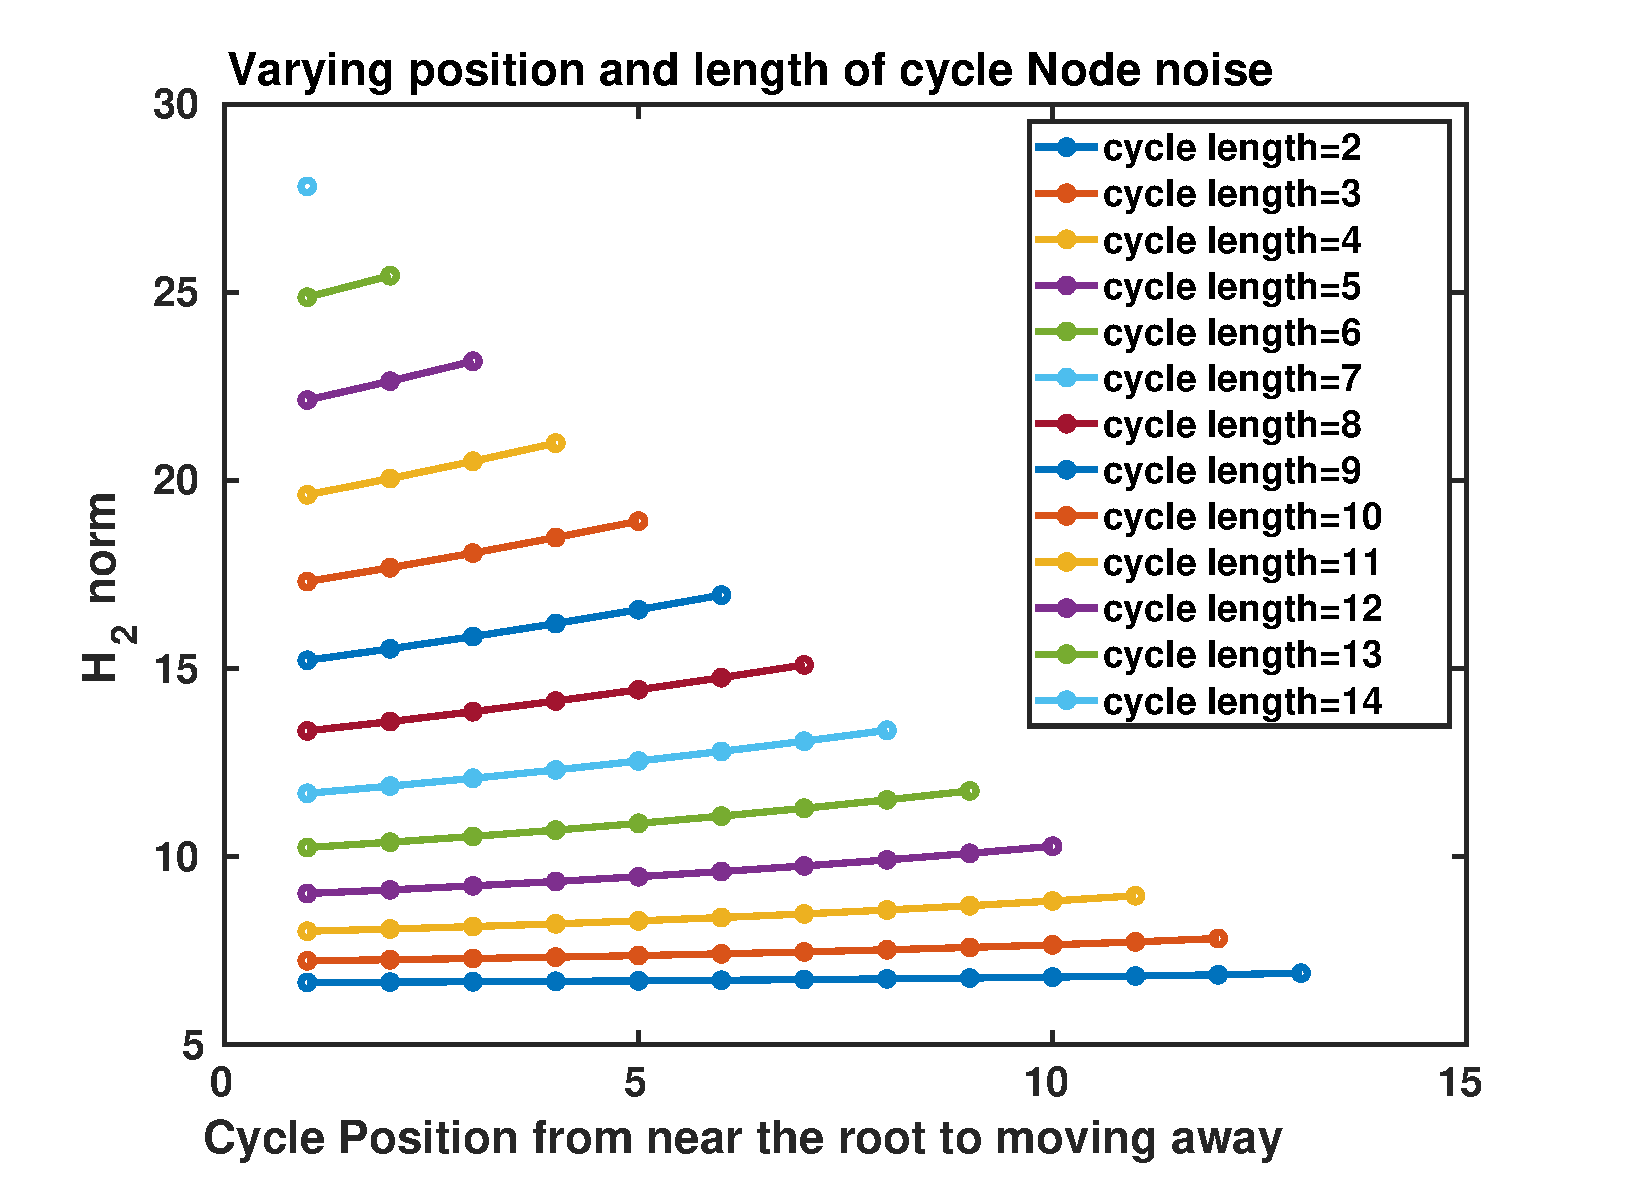
\includegraphics[scale=0.18]{Images/H2normwithvaryingcyclelengthandposition_Nodenoise2.eps}
		\end{figure}
	\end{column}
	\begin{column}{0.3\textwidth}
		\begin{figure}
			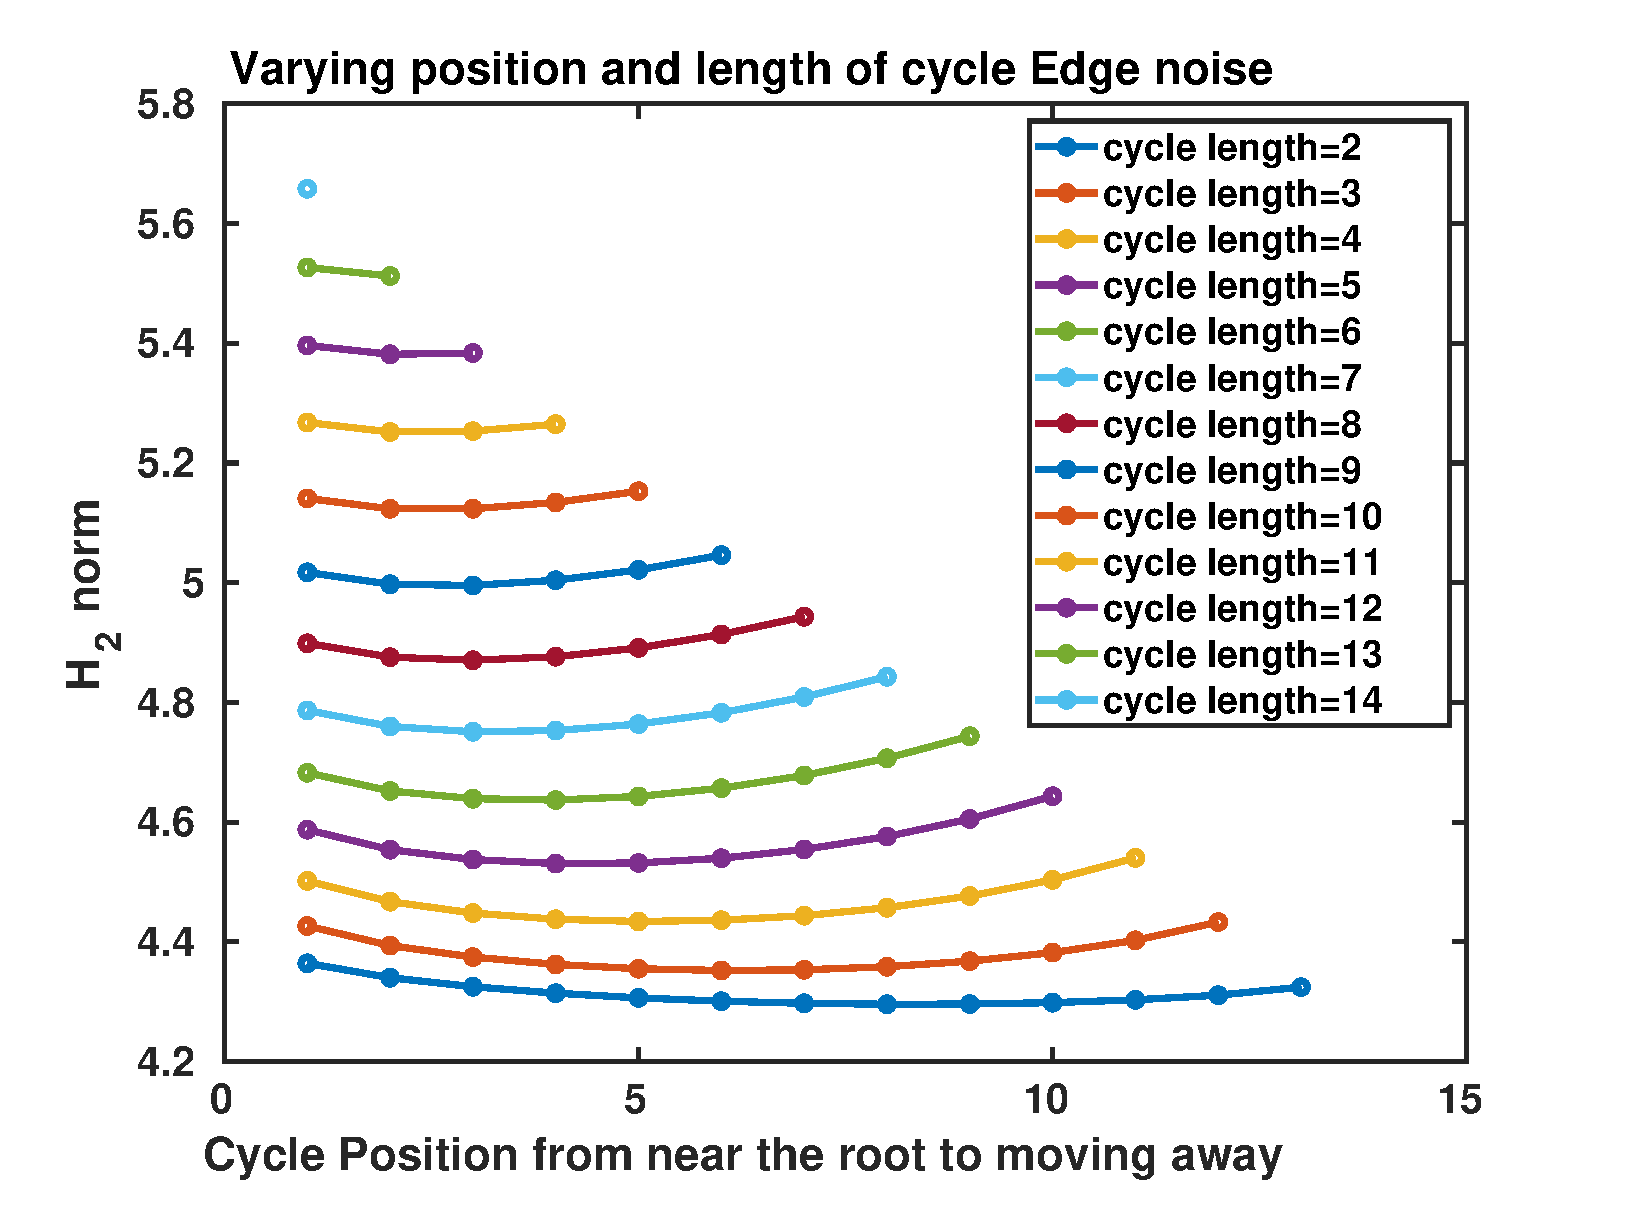
\includegraphics[scale=0.18]{Images/H2normwithvaryingcyclelengthandposition_Edgenoise2.eps}
		\end{figure}
	\end{column}
	\begin{column}{0.3\textwidth}
		\begin{figure}
			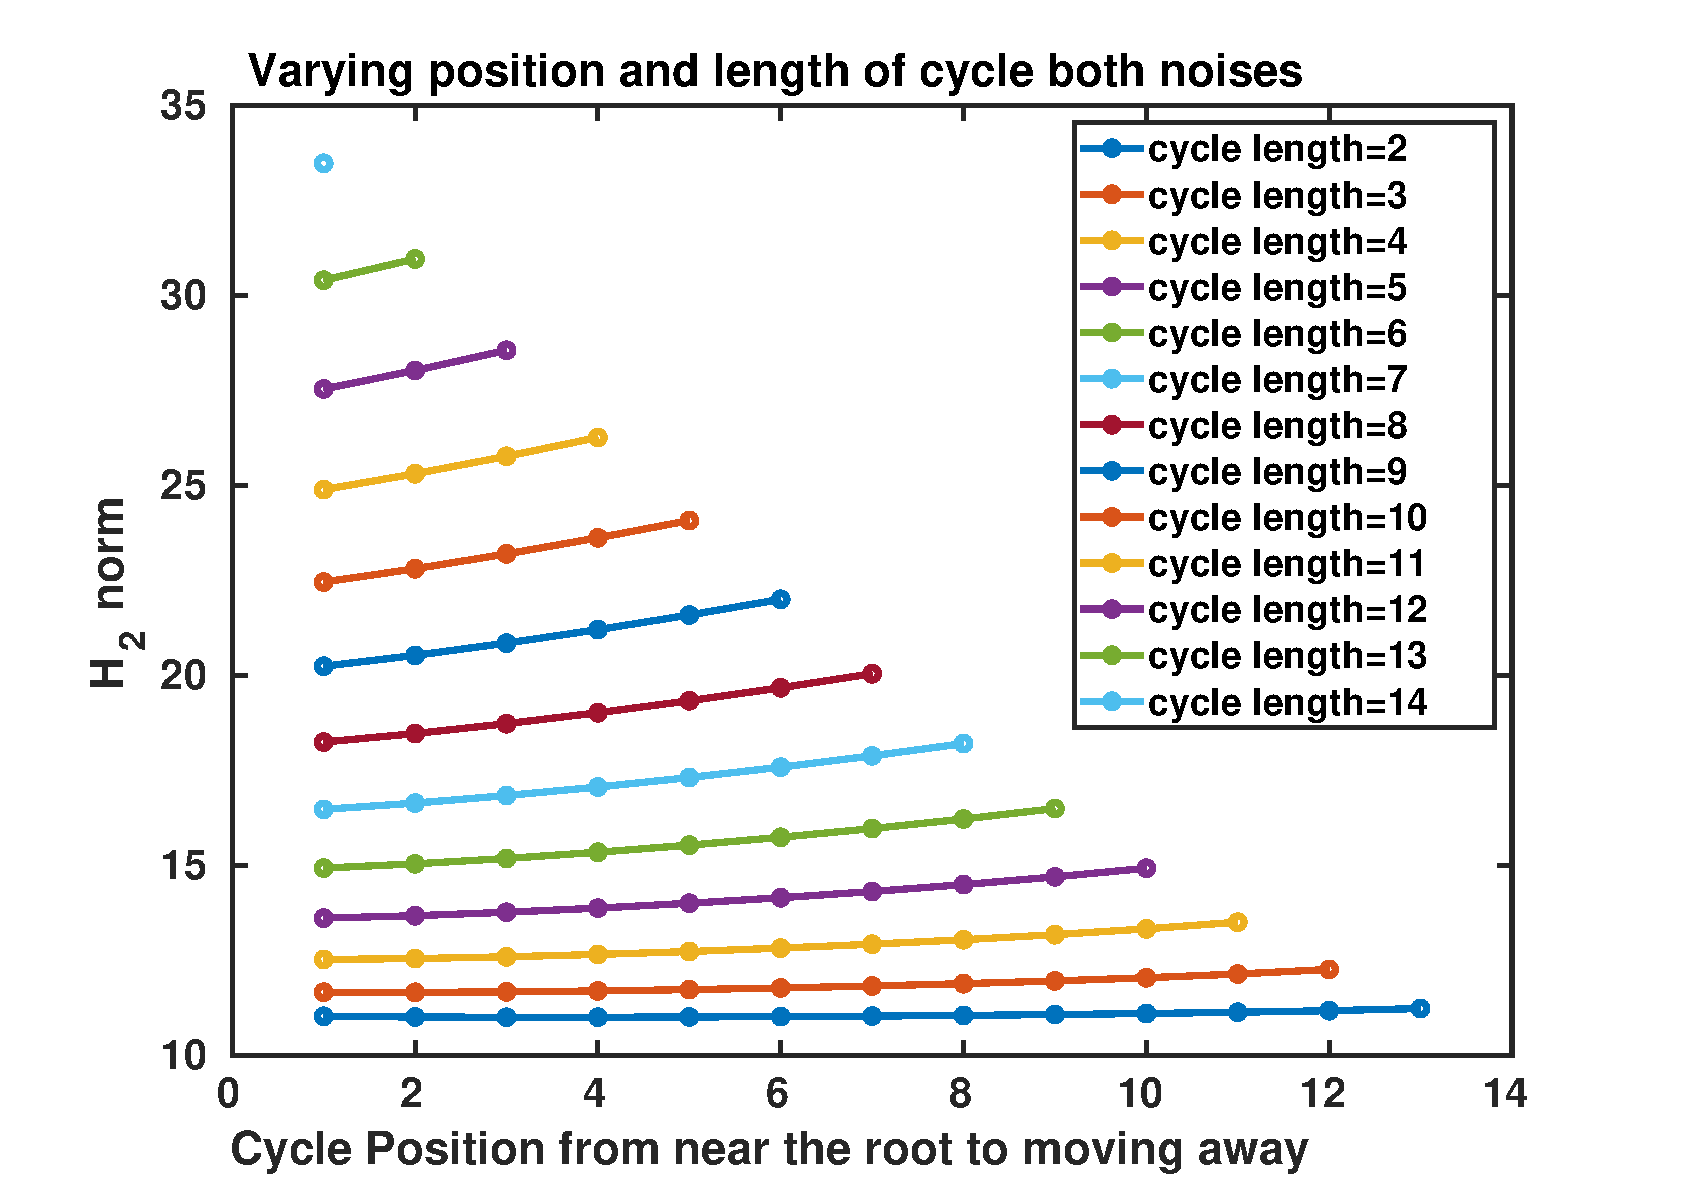
\includegraphics[scale=0.18]{Images/H2normwithvaryingcyclelengthandposition_Bothnoise2.eps}
		\end{figure}
	\end{column}
\end{columns}
\end{frame}
\end{comment}
%%%%%%%%%%%%%%%%%%%%%%%%%%%%%%%%%%%%%%%%%%%%%%%%%%%%
\begin{frame}{}
	\vspace{-0.1cm}
	\begin{block}{Conclusion}
		\begin{columns}
			\vspace{-5cm}
				% Second Column: Single Integrator Undirected Network
			\begin{column}{0.5\textwidth}
				\centering
				\textbf{Network of Single Integrators\footnotemark[1]}
				\begin{itemize}
					\item Longer cycles are better.
					\item Cycle position is not critical to performance.
					\item Choice of Spanning tree has no impact.
					\item $\gamma$ is not a parameter.
					\item Node noise and edge noise not studied separately.
				\end{itemize}
			\end{column}
			% First Column: Double Integrator Directed Network
			\begin{column}{0.5\textwidth}
				\centering
				\textbf{Network of Double Integrators}
				\begin{itemize}
					\item Longer cycles are better.
					\item Cycles at the center of tree are better.
					\item Choice of Spanning tree affect the performance.
					\item Larger values of $\gamma$ are better
					\item Node noise results in variation with cycle position.
				\end{itemize}
			\end{column}
		\end{columns}
	\end{block}
	\footnotetext[1]{\textcolor{blue}{Zelazo, Daniel, Simone Schuler, and Frank Allgöwer.}, {\em "Performance and design of cycles in consensus networks." Systems \& Control Letters 62.1 (2013): 85-96.}}
\end{frame}
\begin{comment}
	\pause
	\begin{block}{Future Work}
		\begin{itemize}
			\item Find analytical solution for directed network.
			\item Study the effects of multiple cycles in the network.
		\end{itemize}
	\end{block}
	
	\vspace{-0.2cm}
		% Second Column: Single Integrator Undirected Network
	\begin{column}{0.35\textwidth}
		\centering
		\textbf{Second Order Directed}
		\begin{itemize}
			\item Shorter cycles are better.
			\item Cycles closer to the root node are better.
			\item Choice of Spanning tree affect the performance.
			\item Larger values of $\gamma$ are better.
			\item Both noises result in positional dependence with Node noise dominating the performance.
		\end{itemize}
	\end{column}
\end{comment}
%%%%%%%%%%%%%%%%%%%%%%%%%%%%%%%%%%%%%%%%%%%%%%%%%%%%
%\section{\color{blue}{Trajectory planning for interception with terminal constraints}}
%%%%%%%%%%%%%%%%%%%%%%%%%%%%%%%%%%%%%%%%%%%%%%%%%%%%%
\begin{frame}[noframenumbering]
	\tableofcontents[currentsection]
	The guidance-related work presented here was carried out under the AR\&DB sponsored project
	“Multi-Vehicular Cooperative Pursuit and Evasion Guidance Strategies: Multi-Agent Perspective”
	(2022–2024)

	\color{magenta}{Principal Investigator: Prof. Shashi Ranjan Kumar}, Department of Aerospace Engineering, IIT Bombay
\end{frame}
%%%%%%%%%%%%%%%%%%%%%%%%%%%%%%%%%%%%%%%%%%%%%%%%%%%%
\begin{frame}{Problem Statement}
	\vspace{-0.5cm}
	%\begin{alertblock}{}
	%Consider a planar interceptor-target engagement geometry as shown. Given an interceptor's launch angle ($\gamma_M$), (constant) speed ($V_M$ ), initial range-to-go ($r$), and maximum lateral acceleration capability ($a^{\rm max}$), design a simple, easy-to-implement guidance law that meets the desired impact/approach angle ($\gamma_T$) and impact/terminal time ($t_{imp}$) requirements.
	%\end{alertblock}
	%\vspace{-0.5cm}
	\begin{figure}
		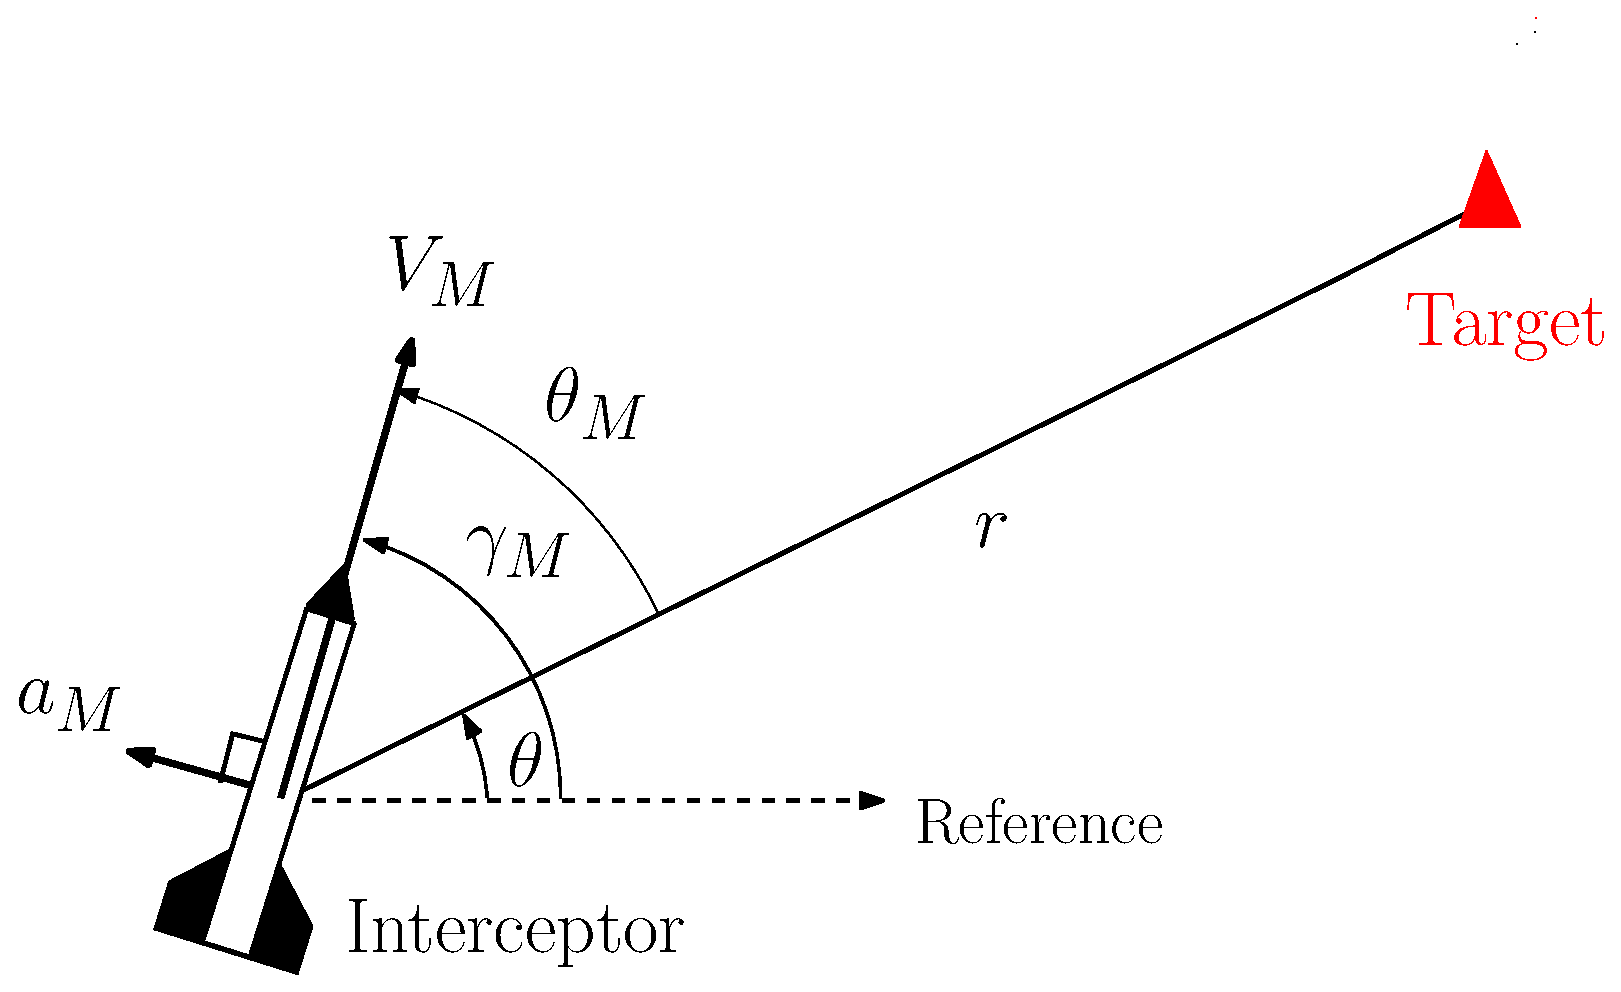
\includegraphics[scale=0.33, keepaspectratio]{Images/dubins_eng.eps}\\
		% \label{ChainLeader}
		% \caption{Engagement scenario against a stationary target.}
	\end{figure} 
	%\vspace{-0.5cm}
	\begin{columns}[T]
		\begin{column}{0.46\textwidth}
			%\column{0.46\textwidth}
			-- \textbf{Geometry: }Planar Engagement\\    
			-- \textbf{Known Parameters: }Launch Angle, Initial Range, Maximum Lateral Acceleration, Speed, \textcolor{red}{Desired Impact Angle and Time}
		\end{column}
		\vrule{}
		\begin{column}{0.5\textwidth}
			%\column{0.5\textwidth}
			-- \textbf{Assumption: } $\theta=0$ \\
			-- \textcolor{blue}{\textbf{Objective: }Design a simple and easy-to-implement guidance law to satisfy the terminal constraints}    
		\end{column}
	\end{columns}
	%\begin{alertblock}{}
	%   We'll consider $\theta=0$ i.e. the target and the launching platform are in the same reference plane. This implies $\gamma_M=\theta_M$ and $\gamma_T=\theta_T$
	%\end{alertblock}
\end{frame}
%%%%%%%%%%%%%%%%%%%%%%%%%%%%%%%%%%%%%%%%%%%%%%%%%%%%%%%%%%%%%%%%%%%%%%%%%%%%%%%%%%%%%%%%%%%%%%%%%
\begin{frame}{Introduction: Why Terminal Constraints Are Important?}
	\begin{figure}
		\centering
		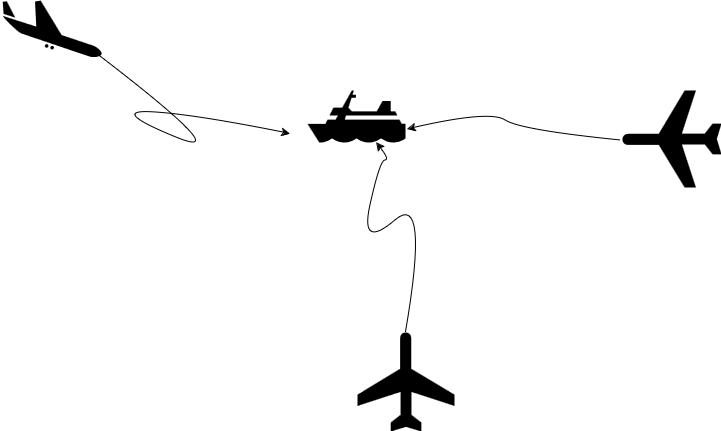
\includegraphics[scale=0.25]{Images/basicattack.png}
	\end{figure}
	\begin{columns}[T]
		\begin{column}{0.59\textwidth}
			%\column{0.46\textwidth}
			-- Exploit the geometric vulnerability\\    
			-- Enhancing warhead effectiveness \\
			-- Exploit fan-shaped coverage zones of radars
		\end{column}
		\vrule{}
		\begin{column}{0.41\textwidth}
			%\column{0.5\textwidth}
			-- Counter defense systems \\
			-- Achieve salvo attack \\
			-- Improve hit-to-kill probability 
		\end{column}
	\end{columns}
	\begin{alertblock}{Simultaneous Control}
		-- Challenging \quad \quad     -- Scarcely examined in the literature
	\end{alertblock}
\end{frame}
%%%%%%%%%%%%%%%%%%%%%%%%%%%%%%%%%%%%%%%%%%%%%%%%%%%%%%%%%%%%%%%%%%%%%%%%%%%%%%%
\begin{frame}{Definitions}
	\begin{defi}[Impact Angle]
		The angle between the velocity vectors of the two adversaries (target and interceptor) at the instant when interception of the target by the interceptor occurs. 
		
		For stationary targets, the impact angle is defined as the angle between the interceptor's velocity vector and some well-defined reference.
	\end{defi}
	\begin{defi}[Impact Time]
		The total time taken after the launch of the interceptor to intercept the target.$$t_{\rm imp}= t_{\rm el} + t_{\rm go},$$ where $t_{\rm el}$ is the time elapsed since the interceptor has been launched, and $t_{\rm go}$ is the time-to-go, i.e., the expected time remaining till interception occurs.
	\end{defi}
\end{frame}

%%%%%%%%%%%%%%%%%%%%%%%%%%%%%%%%%%%%%%%%%%%%%%%%%%%%%
\begin{comment}
\begin{frame}{Dubins Path (1957)\footnotemark[1]}
	\vspace{-0.5cm}
	\begin{columns}[T]%beamer
		\column{0.5\textwidth}
		\begin{defi}
			\justifying
			The shortest curvature bounded path (i.e. $a_M<a_{max}$) between two oriented points is given by a geometric pattern $CCC$ or $CSC$ or a subset of either.
			\begin{itemize}
				\item CSC=$\{LSR, RSL, LSL, RSR\}$
				\item CCC=$\{LRL, RLR\}$
			\end{itemize}
			$C$ - denotes a circular path \\
			$L,R$ - denotes the left and right turning circular paths, respectively. \\
			$S$ - denotes a straight path with zero curvature, i.e., $a_M=0$
		\end{defi}
		\vrule{}
		\column{0.5\textwidth}
		\begin{figure}
			\centering
			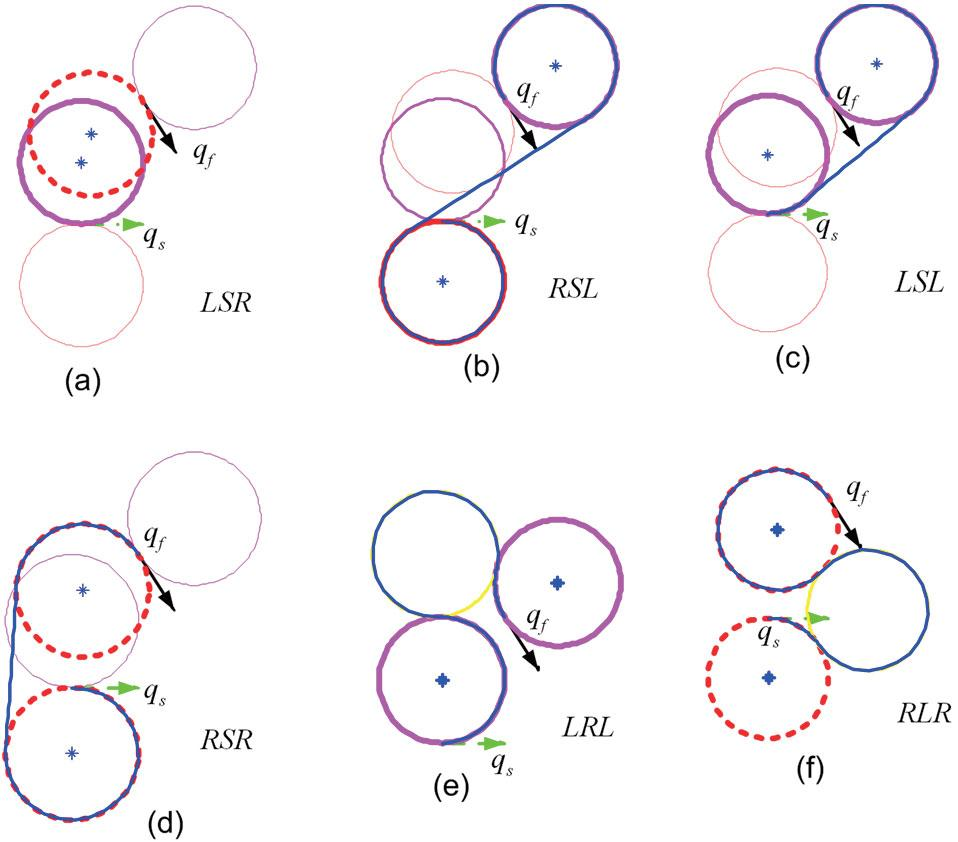
\includegraphics[scale=0.5,width=0.8\textwidth]{Images/dubin.jpeg}
		\end{figure}
	\end{columns}
	\vspace{-0.5cm}
	\footnotetext[1]{Dubins, Lester E. "On curves of minimal length with a constraint on average curvature, and with prescribed initial and terminal positions and tangents." American Journal of mathematics 79.3 (1957): 497-516.}
	\footnotetext[2]{PicSource: I. A. Hameed, "Coverage path planning software for autonomous robotic lawn mower using Dubins' curve," 2017 IEEE International Conference on Real-time Computing and Robotics (RCAR), Okinawa, Japan, 2017, pp. 517-522}
\end{frame}

\end{comment}
%%%%%%%%%%%%%%%%%%%%%%%%%%%%%%%%%%%%%%%%%%%%%%%%%%%%%%%%%%%%%%%%%%%%%%%%%%
\begin{frame}{Dubins Type CLC Path }
	\begin{figure}
		\centering
		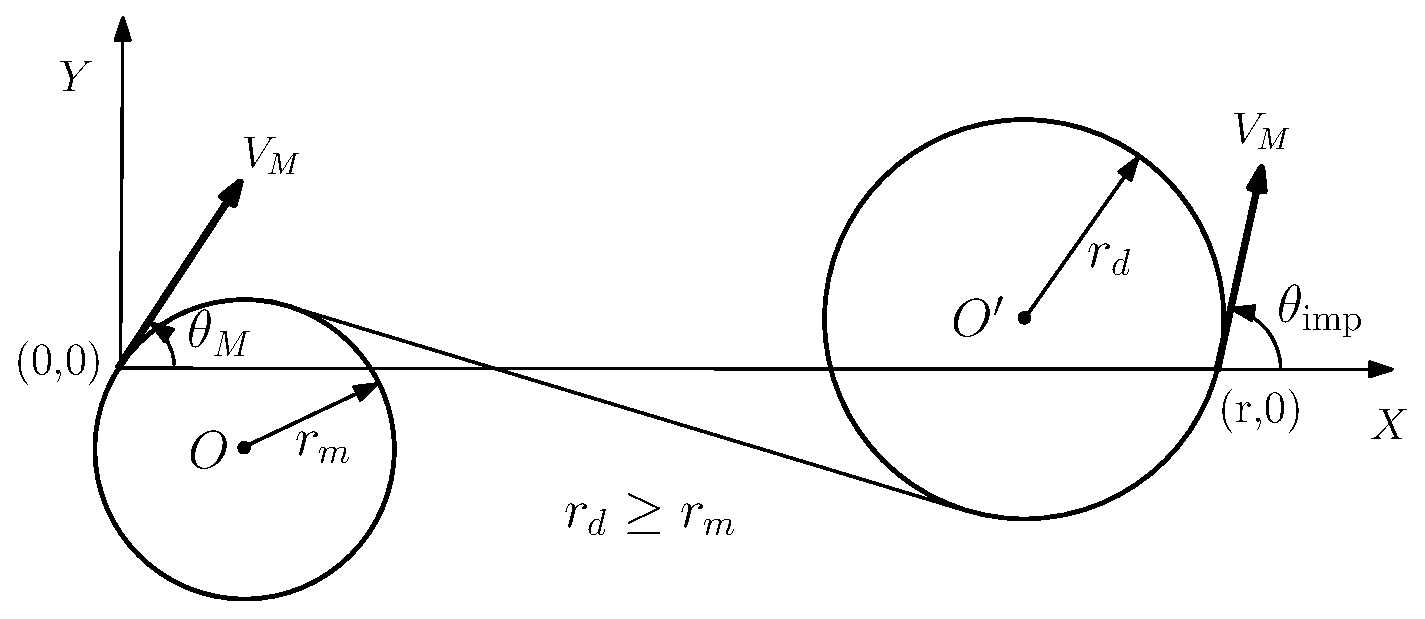
\includegraphics[width=0.4\textwidth, keepaspectratio]{Images/fig1.eps}\\
		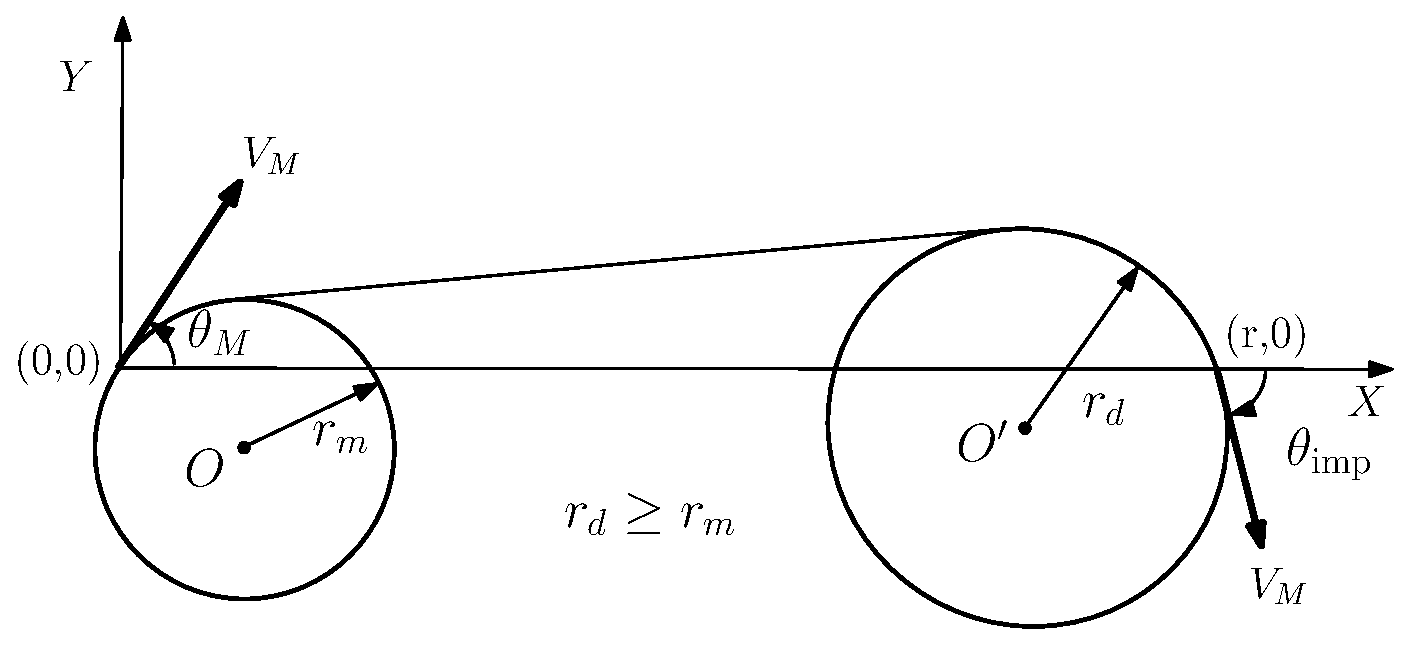
\includegraphics[width=0.4\textwidth, keepaspectratio]{Images/fig2.eps}
		%\caption{Dubins like path with Trasverse Common Tangent (TCT ) and Direct  Common Tangent (DCT)}
	\end{figure}
	%\vspace{-0.5cm}
	%\begin{columns}[T]
	%\column{0.46\textwidth}
	-- TCT based analysis \\    
	-- $C_1$- Constant radius,$C_2$- Variable radius, our design parameter\\
	-- Bounds on TCT and DCT
	%\vrule{}
	%\column{0.5\textwidth}
	%-- \textbf{Assumption: } $\theta=0$ \\
	%-- \textcolor{blue}{\textbf{Objective: }Design a simple and easy-to-implement guidance law to satisfy the terminal constraints}
	%\end{columns}
	%\begin{alertblock}{Note:}
	%   \begin{itemize}
		%      \item In this analysis, we will focus solely on the TCT-based path, as other analyses can be performed similarly and yield nearly identical results.
		%     \item We will maintain the radius of the first circle equal to the minimum turn radius, while using the radius of the second circle as a design parameter to adjust the path length to achieve the desired impact time.
		%    \item The TCT ceases to exist when the circles touch each other, whereas the DCT ceases to exist when one circle is contained within the other.
		% \end{itemize}
	%\end{alertblock}
\end{frame}
%%%%%%%%%%%%%%%%%%%%%%%%%%%%%%%%%%%%%%%%%%%%%%%%%%%%%%%%%%%%%%%%%%%%%%%%%%%%%%%%%%%%%%%%%%%%%
\begin{frame}{TCT Based Path Planning}
	\vspace{-0.3cm}
	\begin{figure}
		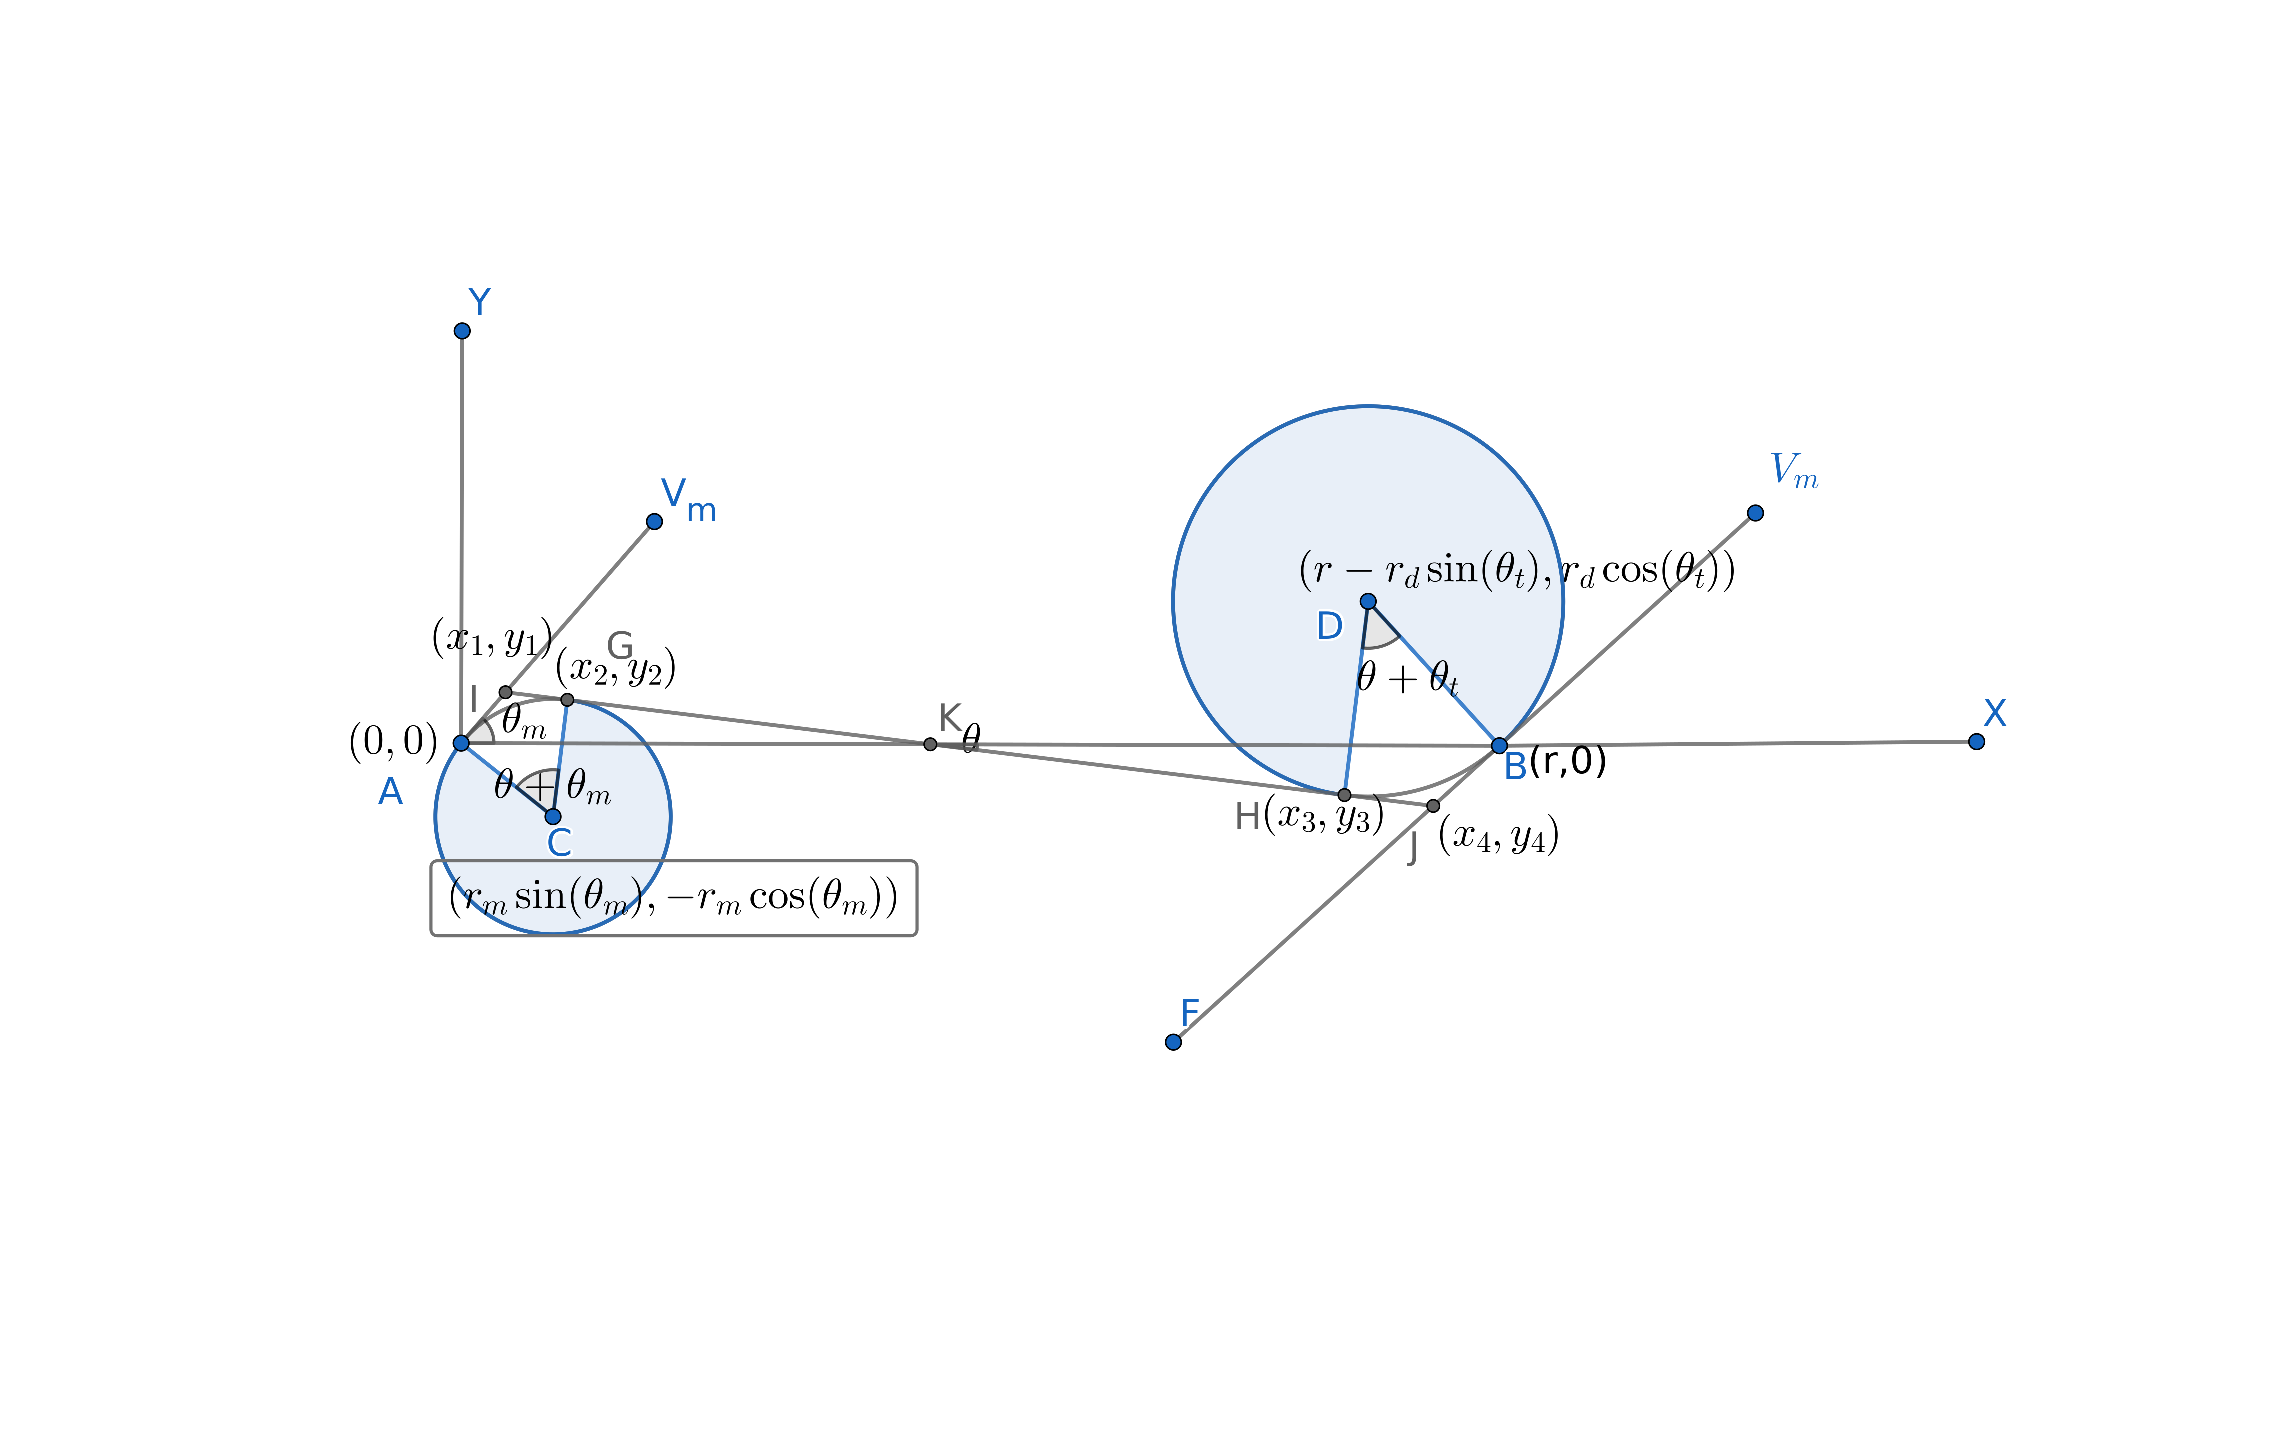
\includegraphics[trim={5cm 6cm 7cm 4cm},clip,width=0.6\textwidth, keepaspectratio]{Images/TCT_final.eps}
		%\caption{The TCT-based Dubins-like path with same-sign angles}
	\end{figure}
	\vspace{-0.3cm}
	\begin{columns}[T]
		\begin{column}{0.45\textwidth}
			%\column{0.45\textwidth}
			Interceptor position - $(0,0)$ \\
			Target position - $(r,0)$\\ 
			Launch angle - $\theta_m \in (0,\pi)$
		\end{column}
		\vrule{}
		\begin{column}{0.5\textwidth}
			%\column{0.5\textwidth}
			Desired impact angle - $\theta_t \in (0,\pi)$ \\
			Scenario with $\theta_m \in (-\pi,0)$\\
			Length IG=$L_{t1}$ and HJ=$L_{t2}$
		\end{column}
	\end{columns}
	\vspace{0.2cm}
	\centering
	$\color{olive}r_{crit}^{TCT}=\frac{r^2-2rr_m\sin\theta_m}{2r_m(1-\cos(\theta_m-\theta_t)+2r\sin\theta_t)} \geq r_d \geq r_m =\frac{V_m^2}{a_{max}}$ \\
\end{frame}
%%%%%%%%%%%%%%%%%%%%%%%%%%%%%%%%%%%%%%%%%%%%%%%%%%%%%%%%%%%%%%%%%%%%%%%%%%%%%%%%%%%%%%%%%%%%%
\begin{frame}{TCT Based Path Planning - Derivation}
	Total path length (P) is $$\color{cyan}r_m(\theta_m+\theta)+\color{magenta}\frac{r-L_{t1}(\cos \theta_m+\cos \theta)-L_{t2}(\cos \theta_t+\cos \theta)}{\cos \theta}+ \color{brown}r_d(\theta_t+\theta)=\color{blue}f(\theta)$$
	\begin{itemize}
		\item $r_d=L_{t2}\cot \frac{\theta_t+\theta}{2}$
		\item $L_{t1}=\frac{c}{\tan \theta_m+\tan \theta}\sec\theta_m$ and $L_{t2}=\frac{c-r\tan \theta}{\tan \theta_t+\tan \theta}\sec\theta_t$
		\item $c=r_m(\cos \theta -\cos \theta_m+\sin \theta \tan \theta+\sin \theta_m \tan \theta)$
	\end{itemize}
	\begin{alertblock}{}
		Given impact time or path length, we can calculate $\theta$ and thus the design parameter $r_d$. \\
		\centering{Is  function $f$ Invertible ?}
	\end{alertblock}
\end{frame}
%%%%%%%%%%%%%%%%%%%%%%%%%%%%%%%%%%%%%%%%%%%%%%%%%%%%%%%%%%%%%%%%%%%%%%%%%%%%%%%%%%%%%%%%%%%%%
\begin{frame}{Path Uniqueness}
	\begin{figure}
		\centering
		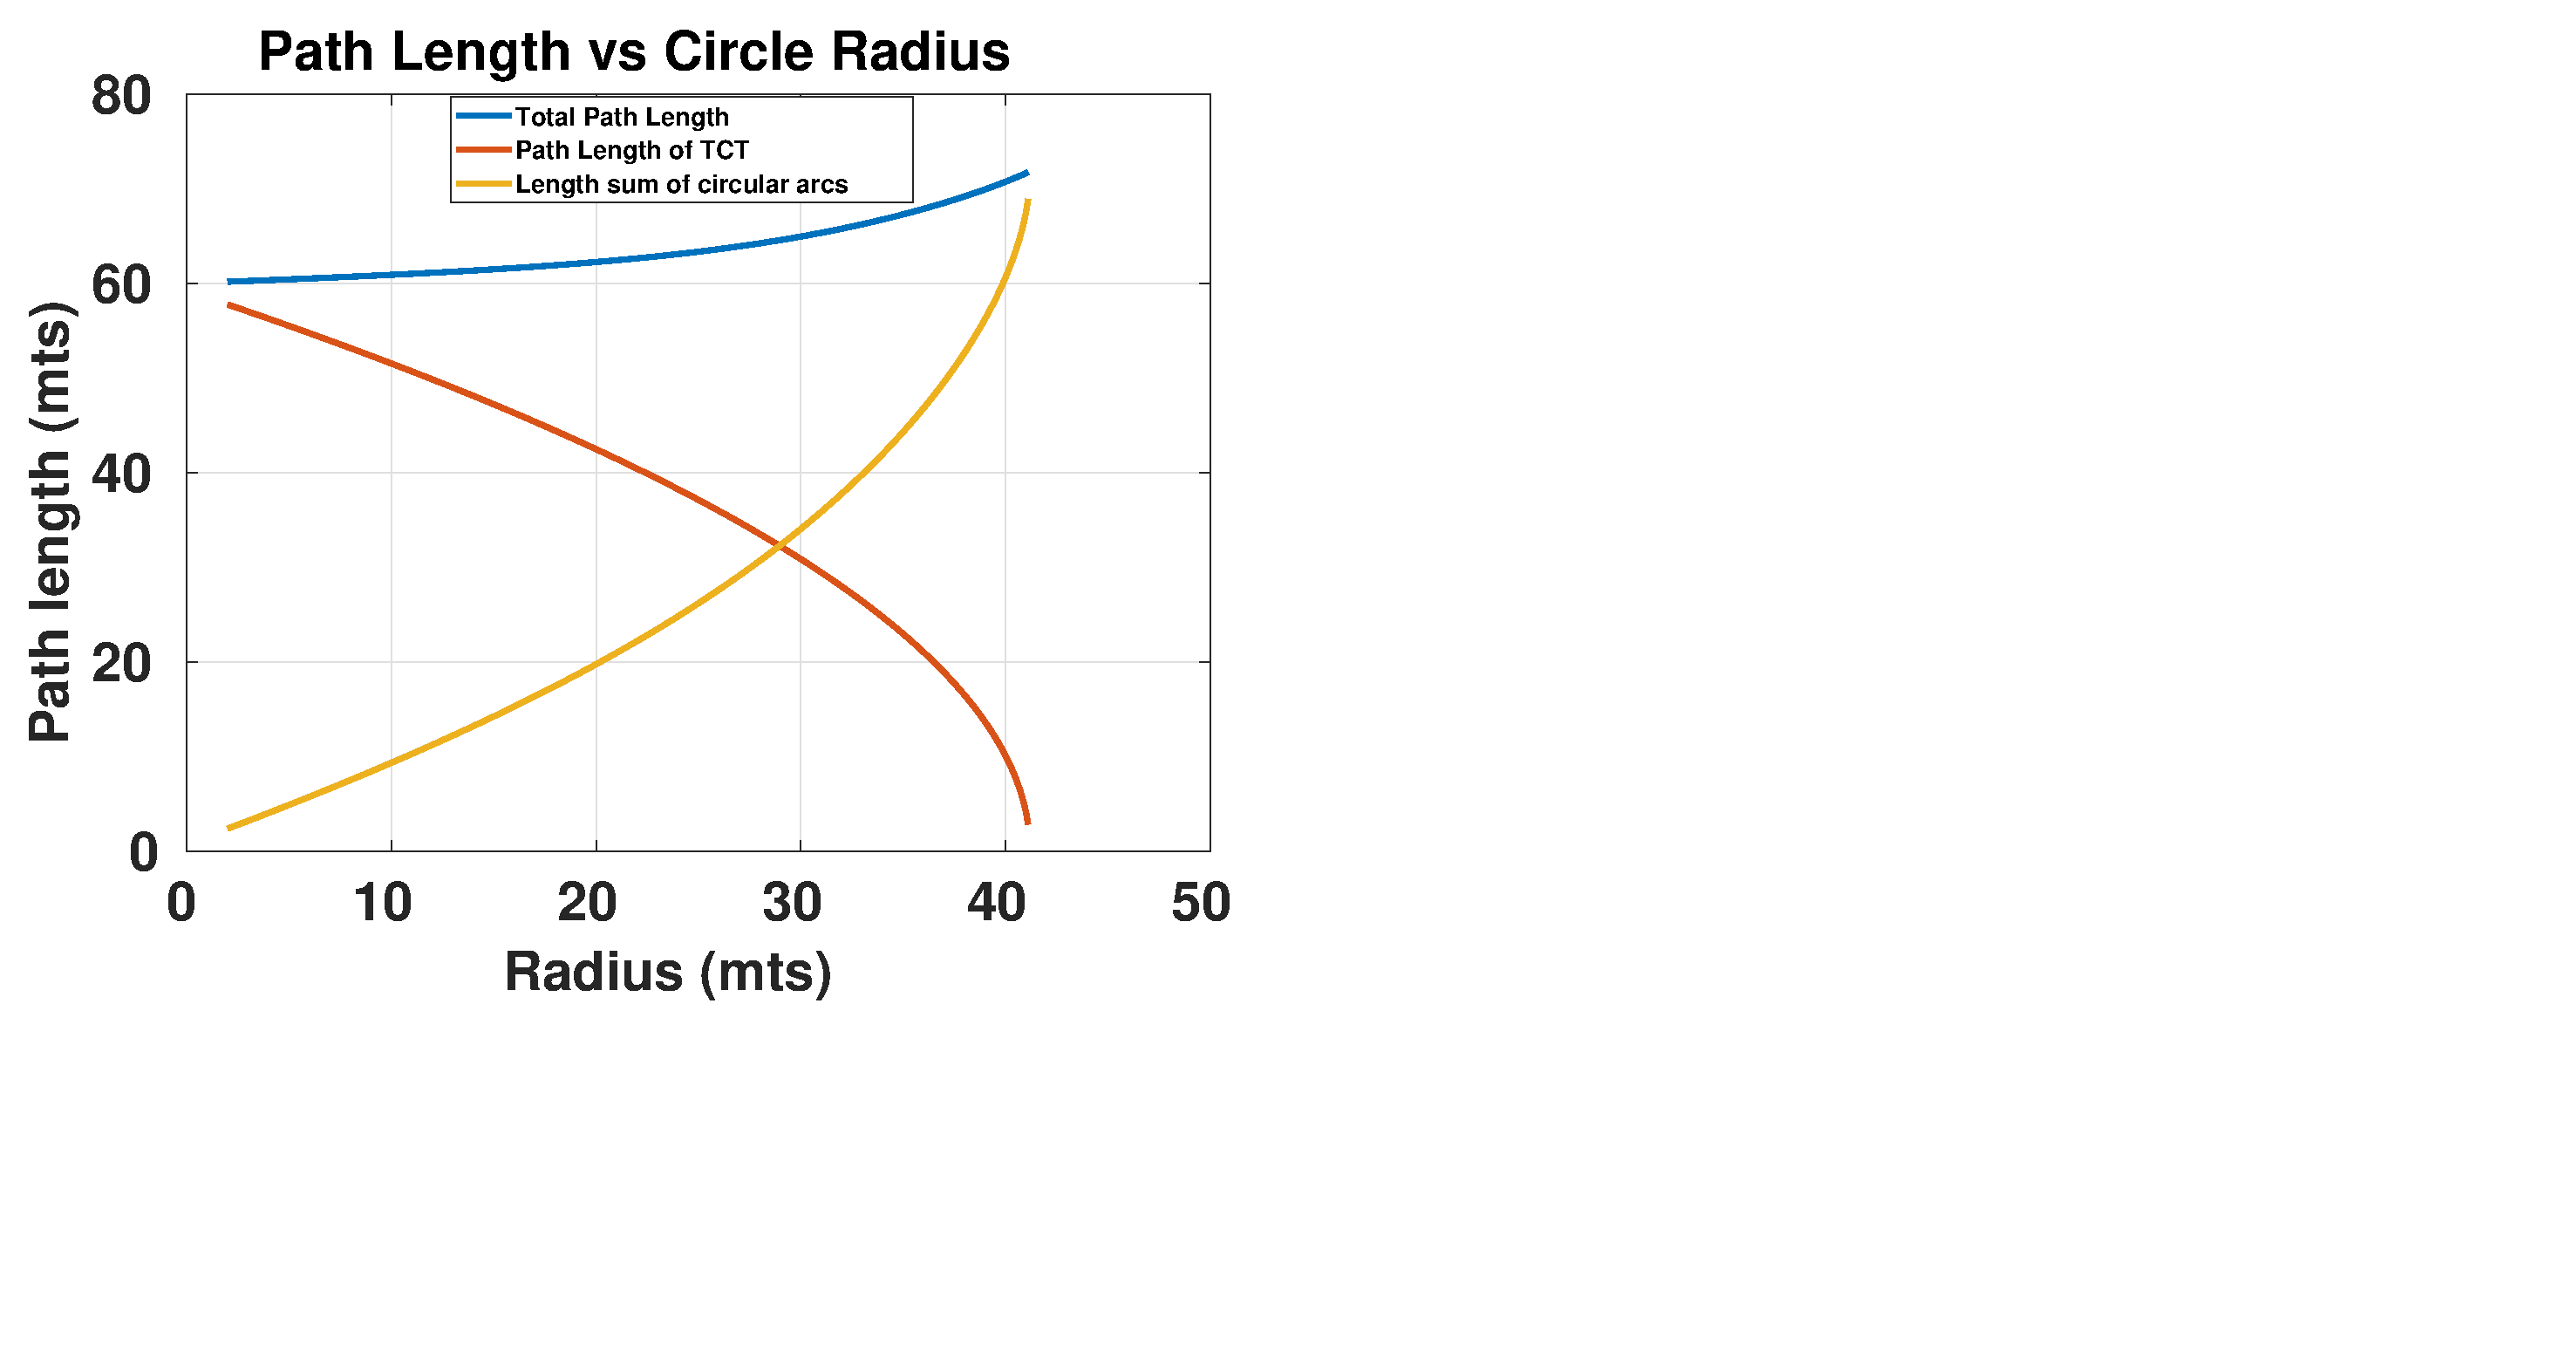
\includegraphics[trim={0cm 6cm 25cm 0cm},clip,scale=0.3]{Images/RadiusVsPathLength1.eps}%{newrad.eps}%
		%\caption{Path length vs radius [$r_d \in (r_m,r_{crit}^{TCT})$]}
		%\label{lengthvsradius}
	\end{figure}
	\vspace{-0.5cm}
	%\begin{block}{Note:}    
	\begin{itemize}
		\item TCT decreases
		\item Arc lengths increases 
		\item Total length Increases
	\end{itemize}
	%\end{block}
\end{frame}
%%%%%%%%%%%%%%%%%%%%%%%%%%%%%%%%%%%%%%%%%%%%%%%%%%%%%%%%%%%%%%%%%%%%%%%%%%%%%%%%%%%%%%%%%%%%%
\begin{comment}
\begin{frame}{TCT Based Path Planning- II}
	\begin{figure}
		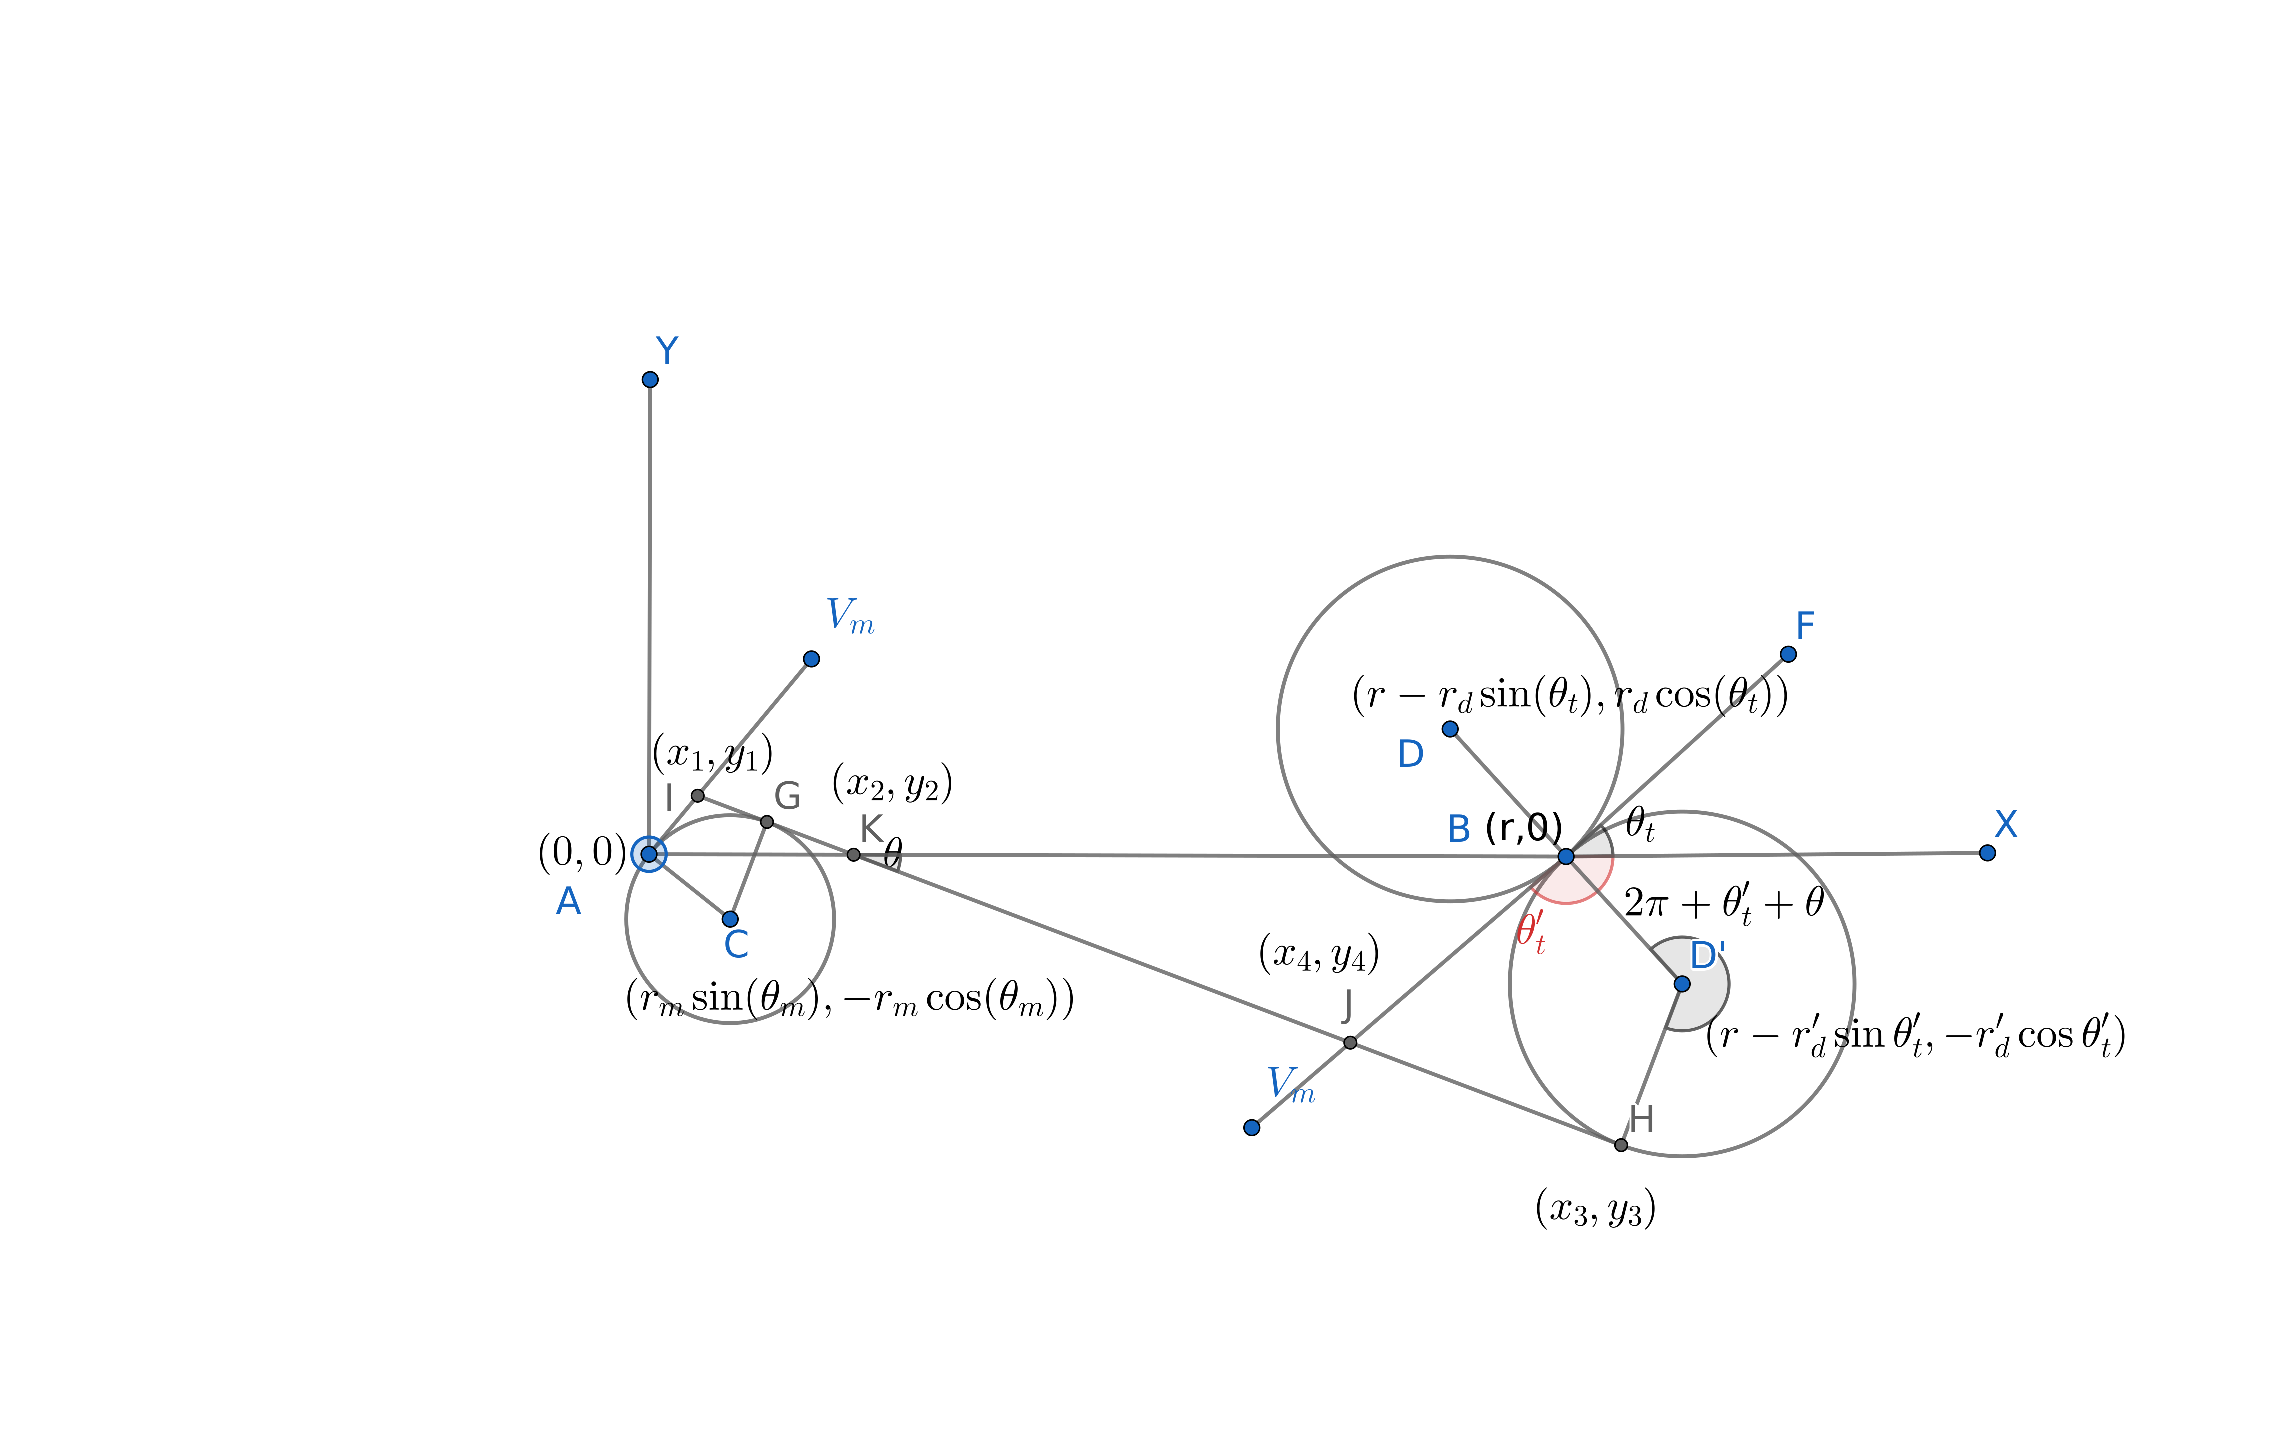
\includegraphics[trim={9cm 2.5cm 2cm 5cm},clip,width=0.7\textwidth]{Images/TCT_EXternal_Final.eps}
		%\caption{The TCT based Dubins like path when both the impact angle and target angle have opposite sign.}
	\end{figure} 
	\vspace{-1cm}
	-- $\theta_t \in (-\pi,0)$ \\
	-- $r_d \in (r_m, \infty)$ \\
	-- If larger impact time is required 
\end{frame}

\end{comment}
%%%%%%%%%%%%%%%%%%%%%%%%%%%%%%%%%%%%%%%%%%%%%%%%%%%%%%%%%%%%%%%%%%%%%%%%%%%%%%%%%%%%%%%%%%%%%
\begin{frame}{Guidance Design} \label{Guidance_Law}
	\begin{block}{}
		The guidance command is proposed as
		\begin{equation*}\label{mainguide}
			a_M=\begin{cases}
				a^{\rm max}\text{sgn}(x),~\text{for}~ 0<t<t_1,\\
				0~\text{for}~t_1<t<t_{1}+t_2\\
				\left(\dfrac{r_m}{r_d}\right)a^{\rm max}\text{sgn}(y)~\text{for}~t_1+t_2<t<t_{1}+t_2+t_3,
			\end{cases}
		\end{equation*}
		-- $t_1,t_1+t_2,t_1+t_2+t_3$ - switching time instants (in seconds)\\
		-- $\text{sgn}(\cdot)$ - the signum function. \\
		-- $x$ and $y$ - arbitrary non-zero real numbers whose signs are opposite.   
	\end{block}
\hyperlink{Dubin_based_Simulation}{\beamerbutton{Simulations}}
\end{frame}

\begin{frame}{Conclusion And Future Work}
	\begin{block}{Conclusion}
		\begin{itemize}
			\item Proposed a simple to implement guidance strategy using piece wise linear accelerations only.
			\item Simultaneously satisfied both the terminal constraints namely Impact Angle and Time.
			\item It was established that launching a vehicle with negative direction to the desired impact angle is advantageous.
		\end{itemize}
	\end{block}
	\textcolor{blue}{Publications: }\\
	\begin{enumerate}
		\item Dubey, A. K., Mukherjee, D., \& Kumar, S. R. (2024, June). Trajectory Planning Using Dubins-Like Paths with Approach Angle and Terminal Time Constraints. In 2024 32nd Mediterranean Conference on Control and Automation (MED) (pp. 412-417). IEEE.
	\end{enumerate}	
\end{frame}

%%%%%%%%%%%%%%%%%%%%%%%%%%%%%%%%%%%%%%%%%%%%%%%%%%%%%%%%%%%%%%%%%%%%%%%%%%%%%%%%%%%%%%%
\begin{subframe}{Simulation Setup}\label{Dubin_based_Simulation}
	\begin{columns}
		\begin{column}{0.5\textwidth}
			-- Desired impact angle $\theta_t=45^\circ$\\
			-- Impact time $t_{imp}=22\,\text{s}$\\
			-- Interceptor's speed $V_m=500\,\text{m/s}$    
		\end{column}
		\vrule{}
		\begin{column}{0.5\textwidth}
			-- Maximum lateral acceleration $a_{max}=400\,\text{m/s}^2$\\
			-- Launch angle $\theta_m=90^\circ$\\
			-- Initial range-to-go $r=10000\,\text{m}$
		\end{column}
	\end{columns}
	\begin{block}{}
		The closed-loop implementation of proposed strategy can be performed using 
		\begin{align}\label{mainguidecl}
			\nonumber a_M=&\frac{a^{\rm max}}{2}\left[\left\{1+\text{sign}(A_1-A)\right\}\text{sgn}(x)\right.\\
			\nonumber &\left.+\left(\frac{r_m}{r_d}\right) \left\{1-\text{sign}(A_1+\ell_{TCT}-A)\right\}\text{sgn}(y)\right], 
		\end{align}
		-- $A$ - Distance (length of the path) traveled by the interceptor since its launch \\
		-- $A_1$ - Distance travelled on circle 1 \\
		-- $\ell_{TCT}$ - Distance travelled on straight line.
	\end{block}
	
\end{subframe}
%%%%%%%%%%%%%%%%%%%%%%%%%%%%%%%%%%%%%%%%%%%%%%%%%%%%%%%%%%%%%%%%%%%%%%%%%%%%%%%%%%%%%%%
\begin{subframe}{Impact Angle $45^\circ$ And Impact Time $22s$}
	\begin{figure}
		%\subfigure[Trajectories.]{\includegraphics[scale=0.75]{trajakd.eps}\hspace{-.2cm}
			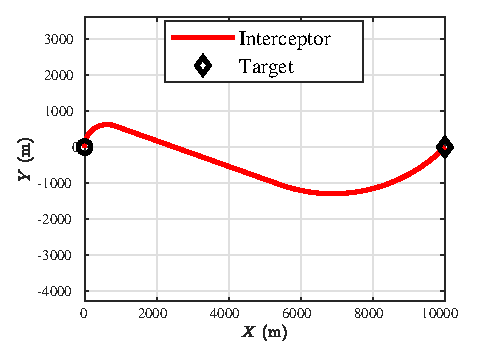
\includegraphics[scale=0.75]{Images/trajakd.eps}
			%\subfigure[$a_M$ and heading angle.]{\includegraphics[scale=0.75]{amsigmakd.eps}
				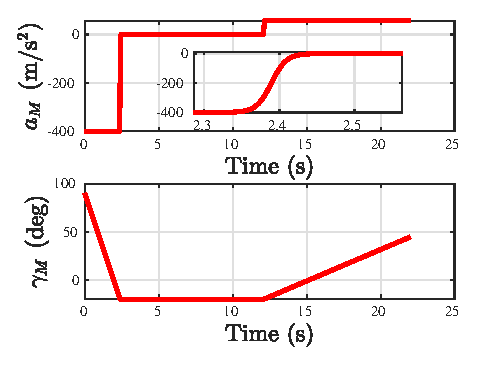
\includegraphics[scale=0.75]{Images/amsigmakd.eps}
				%\caption{Interception of stationary target using TCT at an impact angle of $45^\circ$ and an impact time of 22 seconds.}
	\end{figure}
	\begin{alertblock}{}
				The proposed guidance strategy works for $\theta_m=90^\circ$, whereas, this is not true for many guidance strategies. 
	\end{alertblock}
\end{subframe}
%%%%%%%%%%%%%%%%%%%%%%%%%%%%%%%%%%%%%%%%%%%%%%%%%%%%%%%%%%%%%%%%%%%%%%%%%%%%%%%%%%%%%%%
\begin{subframe}{Impact Angle $45^\circ$ And Different Impact Times}
			\begin{figure}
				%\subfigure[Trajectories.]{\includegraphics[scale=0.55]{traj_tct_compakd.eps}}\hspace{-.2cm}
				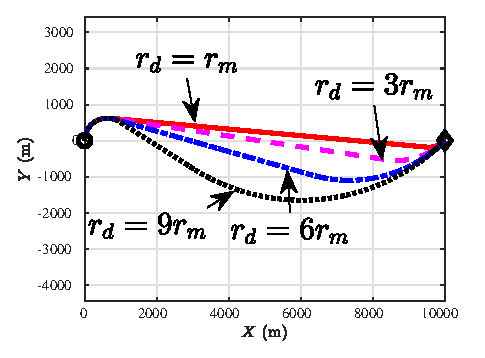
\includegraphics[scale=0.75]{Images/traj_tct_compakd.eps}
				%\subfigure[$a_M$ and heading angle.]{\includegraphics[scale=.23]{amgammam_tct_compsrk.eps}}
				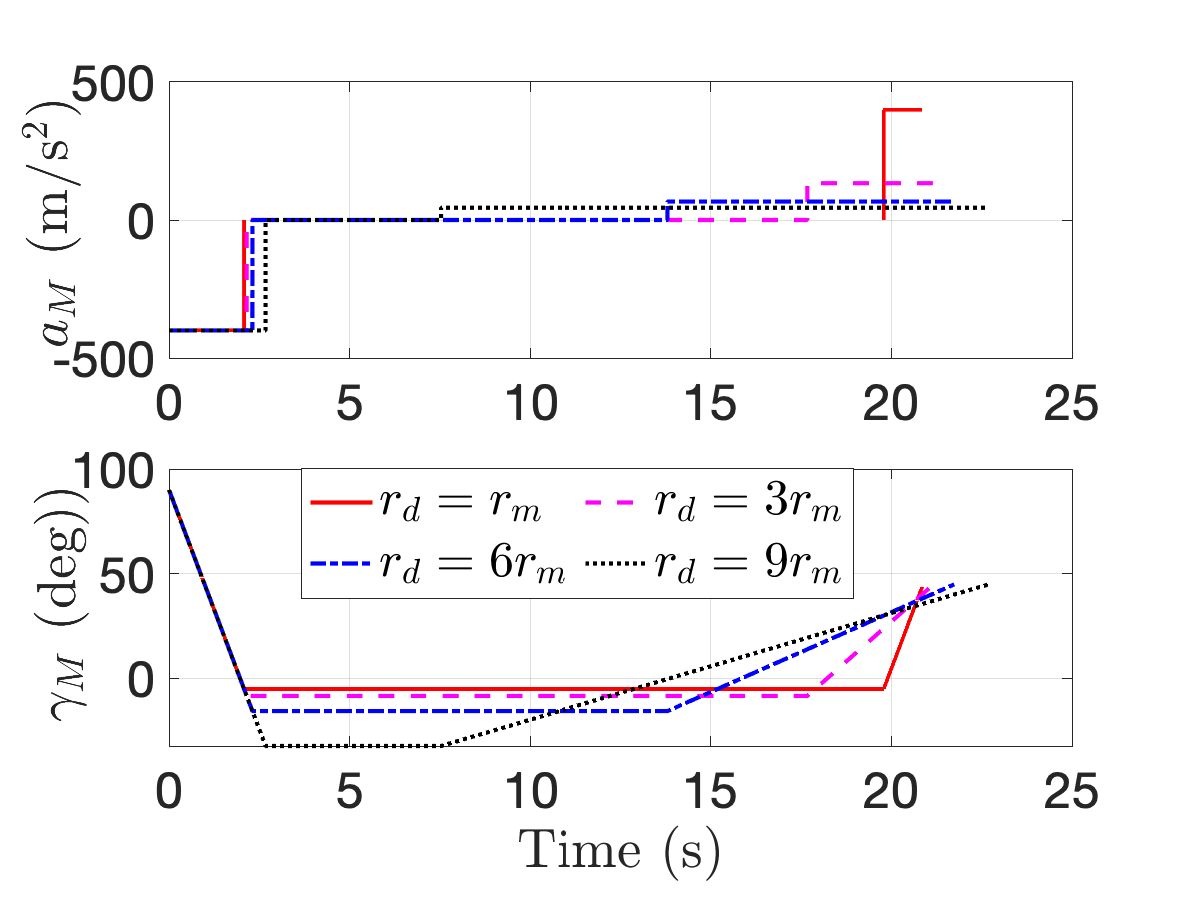
\includegraphics[scale=.3]{Images/amgammam_tct_compsrk.eps}
				%\caption{Interception of stationary target using TCT at an impact angle of $45^\circ$ with different impact times.}
			\end{figure}
\end{subframe}
%%%%%%%%%%%%%%%%%%%%%%%%%%%%%%%%%%%%%%%%%%%%%%%%%%%%%%%%%%%%%%%%%%%%%%%%%%%%%%%%%%%%%%%
\begin{subframe}{Impact Angle $45^\circ$ And Different Impact Times: TCT II}
			\begin{figure}
				\centering
				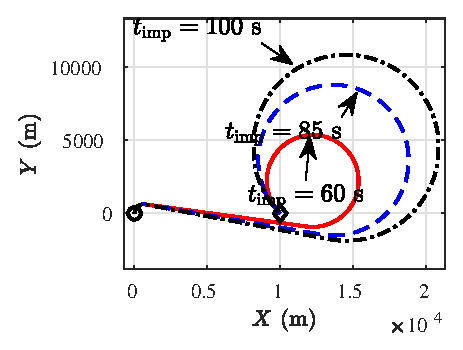
\includegraphics[scale=0.95]{Images/traj_out_tct1akd.eps}
				%\caption{Interception of stationary target using TCT at an impact angle of $45^\circ$ with different impact times when target angle is negative.}
			\end{figure}
			\vspace{-0.5cm}
			\begin{alertblock}{Note:}
				The impact time is unbounded when launched in a direction opposite to the desired impact angle using TCT based approach. 
			\end{alertblock}
\end{subframe}
%%%%%%%%%%%%%%%%%%%%%%%%%%%%%%%%%%%%%%%%%%%%%%%%%%%%%%%%%%%%%%%%%%%%%%%%%%%%%%%%%%%%%%%
\begin{subframe}{Comparison With Existing Strategies}\hyperlink{Guidance_Law}{\beamerbutton{Back2Guidance}}
			\vspace{-0.5cm}
			\begin{figure}
				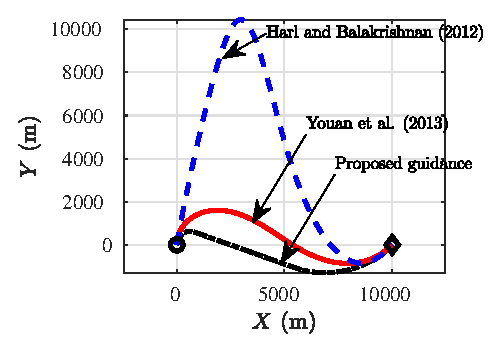
\includegraphics[scale=0.73]{Images/traj_compakd.eps}\hspace{.2cm}
				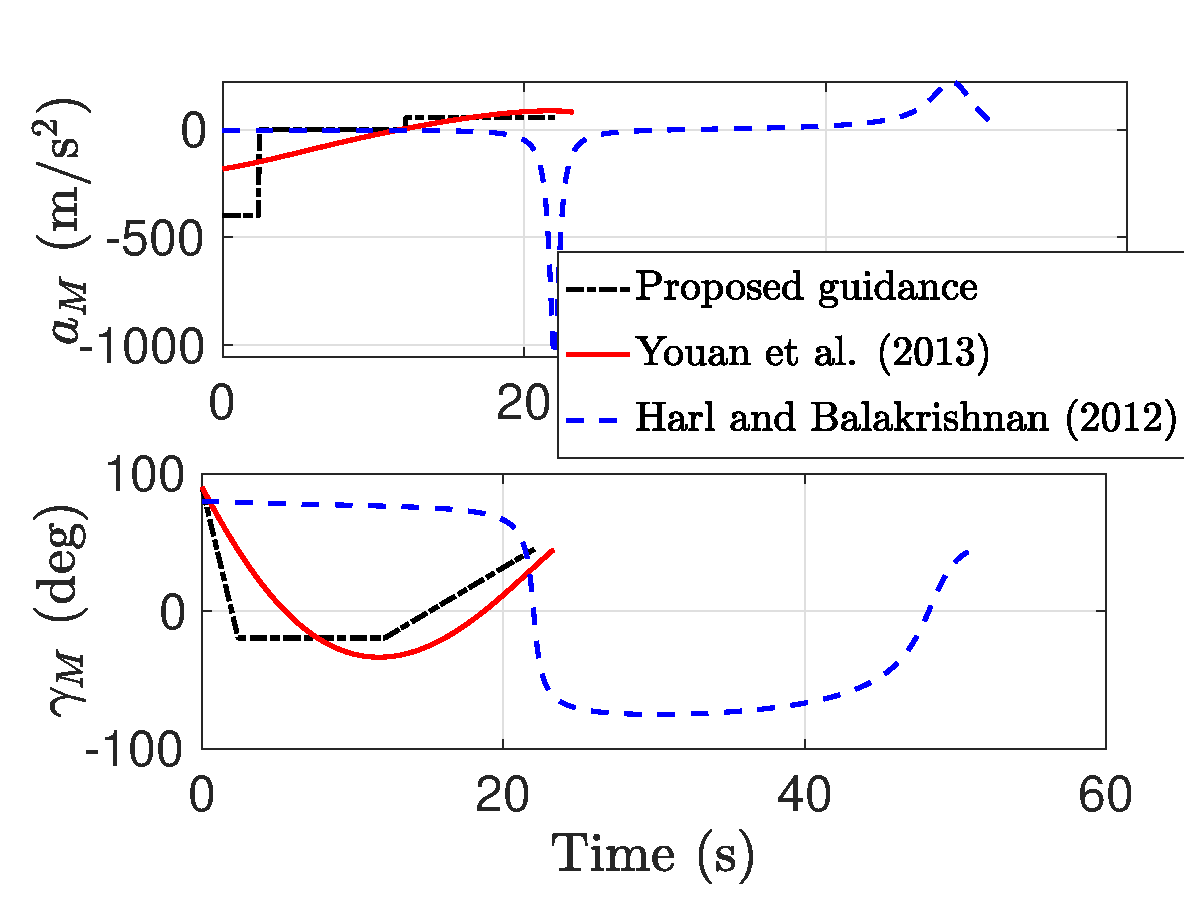
\includegraphics[scale=.3]{Images/am_comp_dubsrk.eps}	
				%\caption{Comparison with existing guidance strategies for an impact angle of $\mp 45^\circ$ and impact time of 22 seconds.}
			\end{figure}
			\vspace{-0.25cm}
			\begin{columns}
				\begin{column}{0.48\textwidth}
					-- \textit{Youan e. al (2013)}\footnotemark[1] 
					\begin{itemize}
						\item Succeeds to intercept when launched at $90^\circ$\\
						\item Exceeds the time requirements.
					\end{itemize}
				\end{column}
				\vrule{}
				\begin{column}{0.52\textwidth}
					-- \textit{Harl And Balakrishnan (2012)}\footnotemark[2]
					\begin{itemize}
						\item Fails to intercept when launched at $90^\circ$\\
						\item $\theta_M=80^\circ$, high impact time.
					\end{itemize}
				\end{column}
			\end{columns}
			\vspace{0.1cm}
			\footnotetext[1]{Zhang, Youan, Guoxin Ma, and Aili Liu. "Guidance law with impact time and impact angle constraints." Chinese Journal of Aeronautics 26.4 (2013): 960-966.}
			\footnotetext[2]{Harl, Nathan, and Sivasubramanya Nadar Balakrishnan. "Impact time and angle guidance with sliding mode control." IEEE Transactions on control systems technology 20.6 (2011): 1436-1449.}

\end{subframe}
%%%%%%%%%%%%%%%%%%%%%%%%%%%%%%%%%%%%%%%%%%%%%%%%%%%%%%%%%%%%%%%%%%%%%%%%%%%%%%%%%%%%%%%
\begin{comment}
	\begin{frame}{Simulation: Variation of the Lateral Acceleration and Impact Time}
		\begin{block}{Future Work}
			\begin{itemize}
			\item To obtain a closed loop implementation
			\item To extend it to multi-body problem for salvo attack.
			\end{itemize}
		\end{block}
				-- $\lambda_{P0}=\pi \quad r_{P0}=100\text{m} \quad V_P=500\,\text{m/s}$\\
				-- For $2000$ pairs $(\zeta_P,p)$ distributed uniformly over grid $[-\pi,\pi]\times[0.1, 1]$
				\vspace{-0.9cm}
				\begin{columns}
					\begin{column}{0.3\textwidth}
						\begin{figure}
							\centering
							\includegraphics[scale=0.5]{Images/t_imp_with_params.eps}
						\end{figure}
					\end{column}
					\begin{column}{0.3\textwidth}
						\begin{figure}
							\centering
							\includegraphics[scale=0.5]{Images/t_imp_with_p.eps}
						\end{figure}
					\end{column}
					\begin{column}{0.3\textwidth}
						--  For a fixed $\zeta_p$, $t_{imp} \downarrow$ when $p \uparrow$
					\end{column}
				\end{columns}
				\vspace{-0.9cm}
				\begin{columns}
					\begin{column}{0.3\textwidth}
						\begin{figure}
							\centering
							\includegraphics[scale=0.5]{Images/a_pmax_with_params.eps}
						\end{figure}
					\end{column}
					\begin{column}{0.3\textwidth}
						\begin{figure}
							\centering
							\includegraphics[scale=0.5]{Images/a_pmax_with_p.eps}
						\end{figure}
					\end{column}
					\begin{column}{0.3\textwidth}
						-- For a fixed $\zeta_p$, U-shaped $a_{P,\max}$ suggests the existence of an optimal trajectory that minimizes the lateral acceleration required.\\
						-- Minima is itself a function of $\zeta_P$\\
						-- No analytical expression for this optimal $p$ exists
					\end{column}
				\end{columns}
	\end{frame}			
\end{comment}
		
		
		
		
		
		
		
		%%%%%%%%%%%%%%%%%%%%%%%%%%%%%%%%%%%%%%%%%%%%%%%%%%%%%%%%%%%%%%%%%%%%%%%%%%%%%%%%%%%%%%%%%%%%%%%%%%%%%%%%
		

%\section{\color{blue}{Spiral Based Pursuer Trajectory for Impact Angle Constraint}}
%%%%%%%%%%%%%%%%%%%%%%%%%%%%%%%%%%%%%%%%%%%%%%%%%%%%%
\begin{frame}[noframenumbering]
	%\tableofcontents[currentsection]
	\begin{center}
		\textcolor{blue}{Problem 3: Spiral Path over Circular Path }
	\end{center}
\end{frame}
%%%%%%%%%%%%%%%%%%%%%%%%%%%%%%%%%%%%%%%%%%%%%%%%%%%%%
\begin{frame}{}
	\vspace{-0.2cm}
	\begin{block}{Well Known Geometric Rules}
		\begin{enumerate}
			\item Pure Pursuit (PP), Deviated Pure Pursuit (DPP) or Proportional Navigation Guidance (PNG): In general does not enforce impact angle. Modified PNG, although enforce the impact angle but same as others requires high terminal acceleration. 
			\item  Polynomial Guidance : The entire path needs to be calculated in the beginning and hence too rigid. 
			\item Circular  and Elliptic Guidance : Simple but Extremely Rigid Path [As our existing Dubins based Path]
%			\item Elliptic Guidance : Same as Circular, Simple but Rigid.
		\end{enumerate}
	\end{block}
	\begin{block}{Spiral Based Laws ($r=\alpha\lambda^\beta$, where $\beta \in (0,1], \alpha \in \mathbb{R}$)}
		\begin{enumerate}
			\item T. Tripathi \& T. Shima [2019]~\footnotemark[1]  : Proposed a geometric rule based on Archimedean spiral ($\beta = 1$) $r(\lambda) = \alpha \lambda$. The geometric rule proposed was $\rm tan (\delta_p) = \lambda_p - \zeta$, where $\zeta$ is the desired impact angle.
			\item K. Mishra \& D. Mukherjee \& S. R. Kumar [2024]~\footnotemark[2]  : Proposed a geometric rule based on generalized spiral $r(\lambda) = \alpha \lambda^\beta$. The geometric rule proposed was $\rm tan (\delta_p) = (\lambda_p - \zeta) / \beta$.
		\end{enumerate}
	\end{block}
	\footnotetext[1]{\textcolor{blue}{Tripathy, T., \& Shima, T. (2019). Archimedean spiral-based intercept angle guidance. Journal of Guidance, Control, and Dynamics, 42(5), 1105-1115.}}
	\footnotetext[2]{\textcolor{blue}{Mishra, K., Mukherjee, D., \& Kumar, S. R. (2024, July). Spiral-based Guidance Strategy for Interception of Stationary Targets. In 2024 American Control Conference (ACC) (pp. 797-802). IEEE.}}
\end{frame}
%%%%%%%%%%%%%%%%%%%%%%%%%%%%%%%%%%%%%%%%%%%%%%%%%%%%%%%%%%%%%%%%%%%%%%%%%%%%%%%
\begin{frame}{Problem Statement}
	\begin{columns}
		\begin{column}{0.4\textwidth}
			\textbf{Engagement Geometry}: Planar
				
			\textbf{Known Parameters: }
			 
			 Launch Angle($\gamma_p$), LOS Angle($\lambda_p$),
			 Deviation or Lead Angle($\delta_p$), 
			 
			 Initial Range($r_0$), Constant Speed($v_p$), 
			 
			 Maximum Lateral Acceleration ($a_{\rm max}$), 
		
			 \textcolor{red}{Desired Impact Angle ($\zeta$)}
			 
			 \textbf{Engagement Kinematics}
			 
			 $\dot{x}_p=v_p \cos(\gamma_p)$, $\dot{y}_p=v_p \sin(\gamma_p)$
			 
			 $\dot{\gamma}_p=a_p/v_p$ 
			 
			 $r_p\dot{\lambda}_p = -v_p\sin(\gamma_p - \lambda_p) = -v_p \sin(\delta_p)$
			 
			 $\dot{\r}_p = -v_p\cos(\gamma_p - \lambda_p) = -v_p \cos(\delta_p)$
			 
			 
			 
		\end{column}
		\begin{column}{0.6\textwidth}
					\begin{figure}
				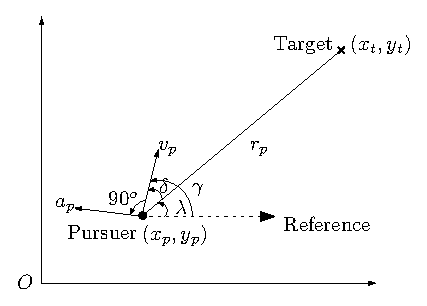
\includegraphics[scale=0.9, keepaspectratio]{Images/Eng_geom.eps}\\
				% \label{ChainLeader}
				% \caption{Engagement scenario against a stationary target.}
			\end{figure}
			
		\end{column}
	\end{columns}
		\begin{alertblock}{}
		%	 Given a pursuer's launch angle ($\gamma_p$), (constant) speed ($v_p$ ), initial range-to-go ($r_0$), and maximum lateral acceleration capability ($a_{\rm max}$), design a simple, easy-to-implement guidance law that meets the desired impact/approach angle ($\zeta$).
		\textcolor{blue}{\textbf{Objective: }\\
			Design a simple and easy-to-implement guidance law to satisfy the impact angle constraint}
	\end{alertblock}	
\end{frame}
%%%%%%%%%%%%%%%%%%%%%%%%%%%%%%%%%%%%%%%%%%%%%%%%%%%%%
\begin{comment}

\begin{frame}{Introduction: Why Impact Angle Constraints Are Important?}
	\begin{columns}
		\hspace*{0.2cm}
		\begin{column}{0.5\textwidth}
			\begin{defi}[Impact Angle]
				\begin{itemize}
					\item The angle between the velocity vectors of the two adversaries (target and interceptor) at the instant when interception of the target by the interceptor occurs. 
					\item For stationary targets, the impact angle is defined as the angle between the interceptor's velocity vector and some well-defined reference.
				\end{itemize}
			\end{defi}
		\end{column}
		\begin{column}{0.5\textwidth}
			\begin{figure}
				\centering
				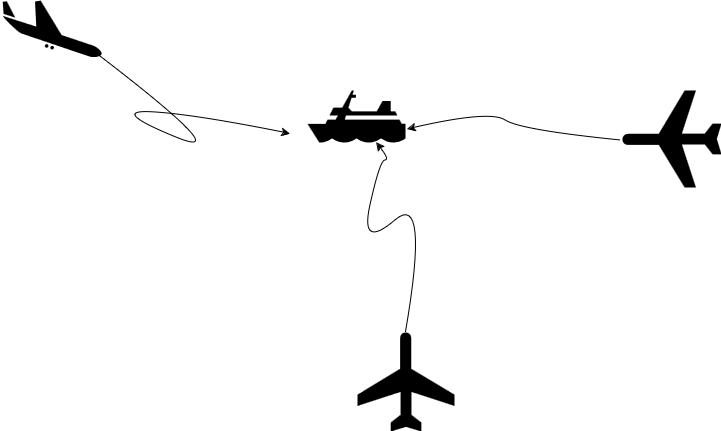
\includegraphics[scale=0.25]{Images/basicattack.png}
			\end{figure}
		\end{column}
	\end{columns}
	\vspace{0.5cm}
	\begin{columns}[T]
		\begin{column}{0.59\textwidth}
			%\column{0.46\textwidth}
			-- Exploit the geometric vulnerability\\    
			-- Enhancing warhead effectiveness \\
			-- Exploit fan-shaped coverage zones of radars
		\end{column}
		\vrule{}
		\begin{column}{0.41\textwidth}
			%\column{0.5\textwidth}
			-- Counter defense systems \\
			-- Improve hit-to-kill probability 
		\end{column}
	\end{columns}
\end{frame}


%%%%%%%%%%%%%%%%%%%%%%%%%%%%%%%%%%%%%%%%%%%%%%%%%%%%%
\begin{frame}{Literature Survey}
	\vspace{-0.2cm}
\begin{block}{Well Known Geometric Rules}
	\begin{enumerate}
		\item Pure Pursuit (PP), Deviated Pure Pursuit (DPP) or Proportional Navigation Guidance (PNG): In general does not enforce impact angle. Modified PNG, although enforce the impact angle but same as others requires high terminal acceleration. 
		\item  Polynomial Guidance : The entire path needs to be calculated in the beginning and hence too rigid. 
		\item Circular Navigation Guidance : Simple but Extremely Rigid Path
		\item Elliptic Guidance : Same as Circular, Simple but Rigid.
	\end{enumerate}
\end{block}
	\begin{block}{Spiral Based Laws ($r=\alpha\lambda^\beta$, where $\beta \in (0,1], \alpha \in \mathbb{R}$)}
		\begin{enumerate}
			\item T. Tripathi \& T. Shima [2019]~\footnotemark[1]  : Proposed a geometric rule based on Archimedean spiral ($\beta = 1$) $r(\lambda) = \alpha \lambda$. The geometric rule proposed was $\rm tan (\delta_p) = \lambda_p - \zeta$, where $\zeta$ is the desired impact angle.
			\item K. Mishra \& D. Mukherjee \& S. R. Kumar [2024]~\footnotemark[2]  : Proposed a geometric rule based on generalized spiral $r(\lambda) = \alpha \lambda^\beta$. The geometric rule proposed was $\rm tan (\delta_p) = (\lambda_p - \zeta) / \beta$.
		\end{enumerate}
	\end{block}
	\footnotetext[1]{\textcolor{blue}{Tripathy, T., \& Shima, T. (2019). Archimedean spiral-based intercept angle guidance. Journal of Guidance, Control, and Dynamics, 42(5), 1105-1115.}}
	\footnotetext[2]{\textcolor{blue}{Mishra, K., Mukherjee, D., \& Kumar, S. R. (2024, July). Spiral-based Guidance Strategy for Interception of Stationary Targets. In 2024 American Control Conference (ACC) (pp. 797-802). IEEE.}}
\end{frame}
\end{comment}
%%%%%%%%%%%%%%%%%%%%%%%%%%%%%%%%%%%%%%%%%%%%%%%%%%%%%
\begin{frame}{Curvature Vs Alpha}
	\vspace{-0.2cm}
	\begin{block}{Problems with the proposed laws}
		\begin{itemize}
			\item The proposed laws are independent of the spiral parameter $\alpha$ and the parameter $\alpha = r_0 / (\lambda_0 - \zeta)^\beta$ depends on initial Launch Angle and the initial Radial distance. Both of which are not usually a parameter of choice. 
		\end{itemize}
	\end{block}
	\begin{columns}
		\begin{column}{0.45\textwidth}
			$\kappa=\frac{\theta^{1-\beta}(\beta^2+\beta+\theta^2)}{\alpha(\beta^2+\theta^2)^{1.5}}$,
			\vspace{0.1cm}
			$\kappa_{max}=\frac{(3\beta^2+1)^{0.5}+\beta-1}{\alpha((3\beta^2+1)^{0.5}-1-\beta^2)^{(\beta-1)/2}((3\beta^2+1)^{0.5}-1)^{1.5}}$
			\vspace{0.1cm}
			$\kappa_{max}=\frac{f(\beta)}{\alpha}$
			
			\vspace{0.2cm}
			The curvature as well as maximum curvature and hence the Latax ($a=v_p^2\kappa$) is inversely proportional to $\alpha$.
		\end{column}
		\begin{column}{0.54\textwidth}
			\begin{figure}
				\centering
				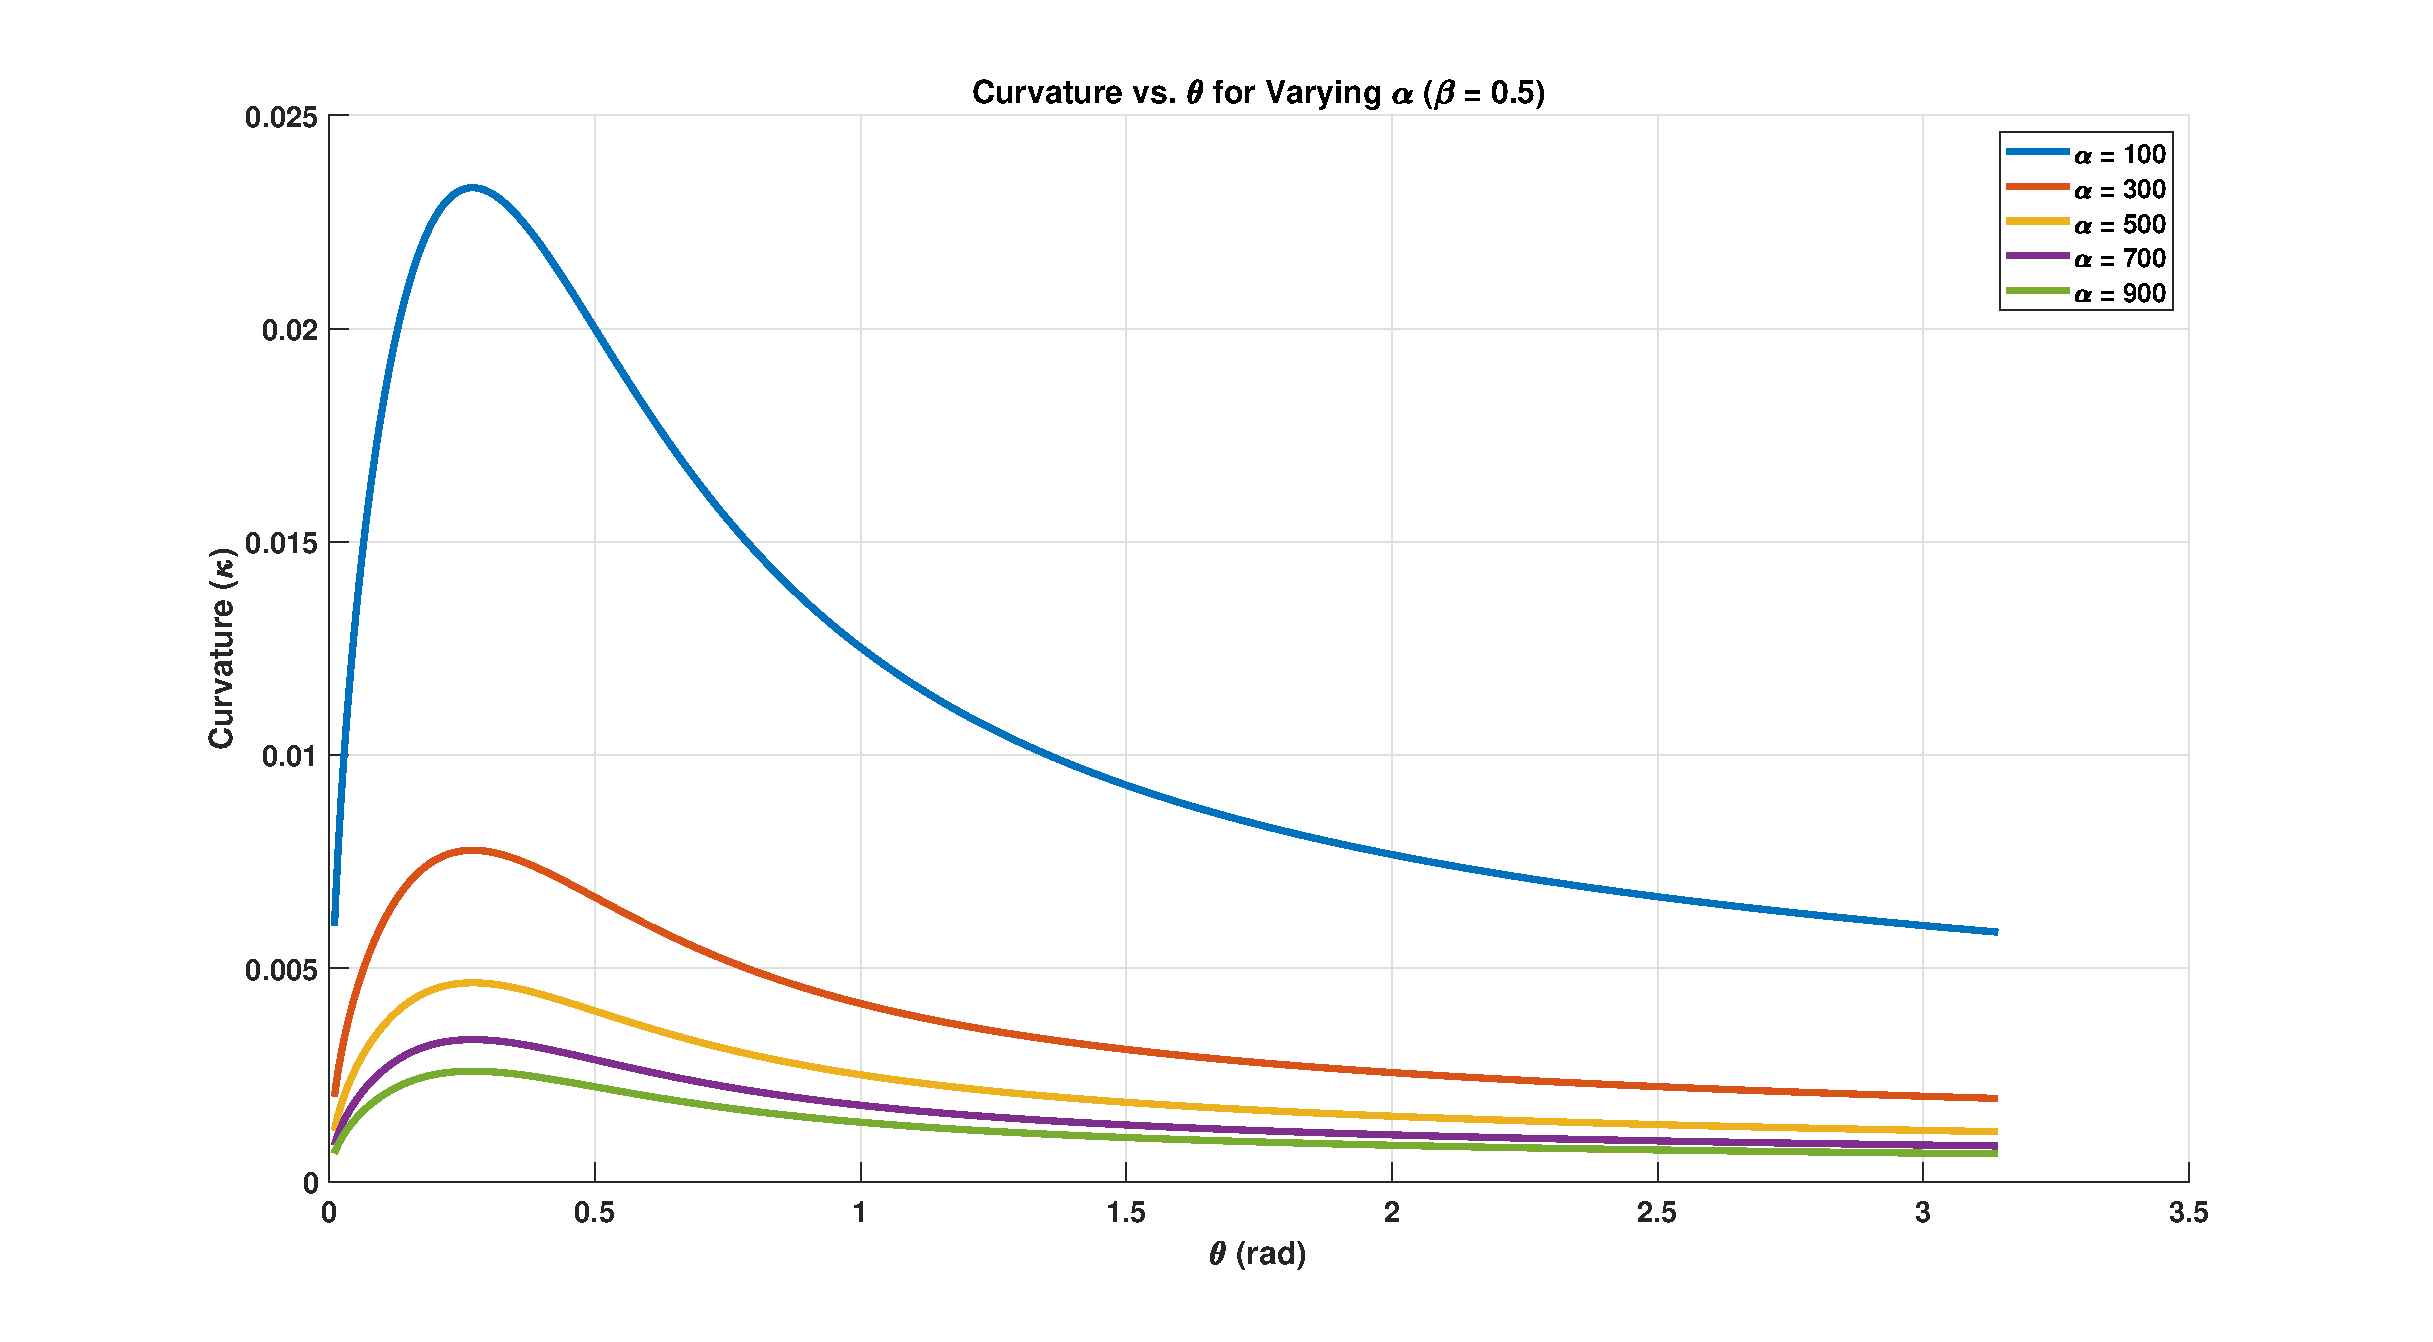
\includegraphics[scale=0.2]{Images/CurvVsAngle_FixedBeta_VaryingAlpha.eps}
			\end{figure}
		\end{column}
	\end{columns}
%	\vspace{-1.0 cm}
%\begin{columns}
%	\begin{column}{0.5\textwidth}
%		\begin{figure}
%			\centering
%			\includegraphics[scale=0.2]{CurvVsAngle_FixedAlpha_VaryingBeta.eps}
%		\end{figure}
%			The curvature as well as maximum curvature and hence the Latax is directly proportional to $\beta$ as shown.
%	\end{column}
%	\begin{column}{0.5\textwidth}
%	\end{column}
%\end{columns}
\end{frame}
%%%%%%%%%%%%%%%%%%%%%%%%%%%%%%%%%%%%%%%%%%%%%%%%%%%%%
\begin{frame}{Problem Demonstration}
	\vspace{-0.2cm}
	\begin{alertblock}{Inappropriate $\alpha$}
		If the initial value of $\alpha$ is not appropriate, the constrained lateral acceleration i.e. Latax (e.g. 30G) may not be sufficient to achieve the target. 
	\end{alertblock}
	The plot below reproduce the example demonstrated in the paper by K. Mishra \& D. Mukherjee \& S.R. Kumar~\footnotemark[1] by applying the constrained Latax.
	\vspace{-0.7cm} 
	\begin{columns}
		\begin{column}{0.5\textwidth}
			\begin{figure}
				\centering
				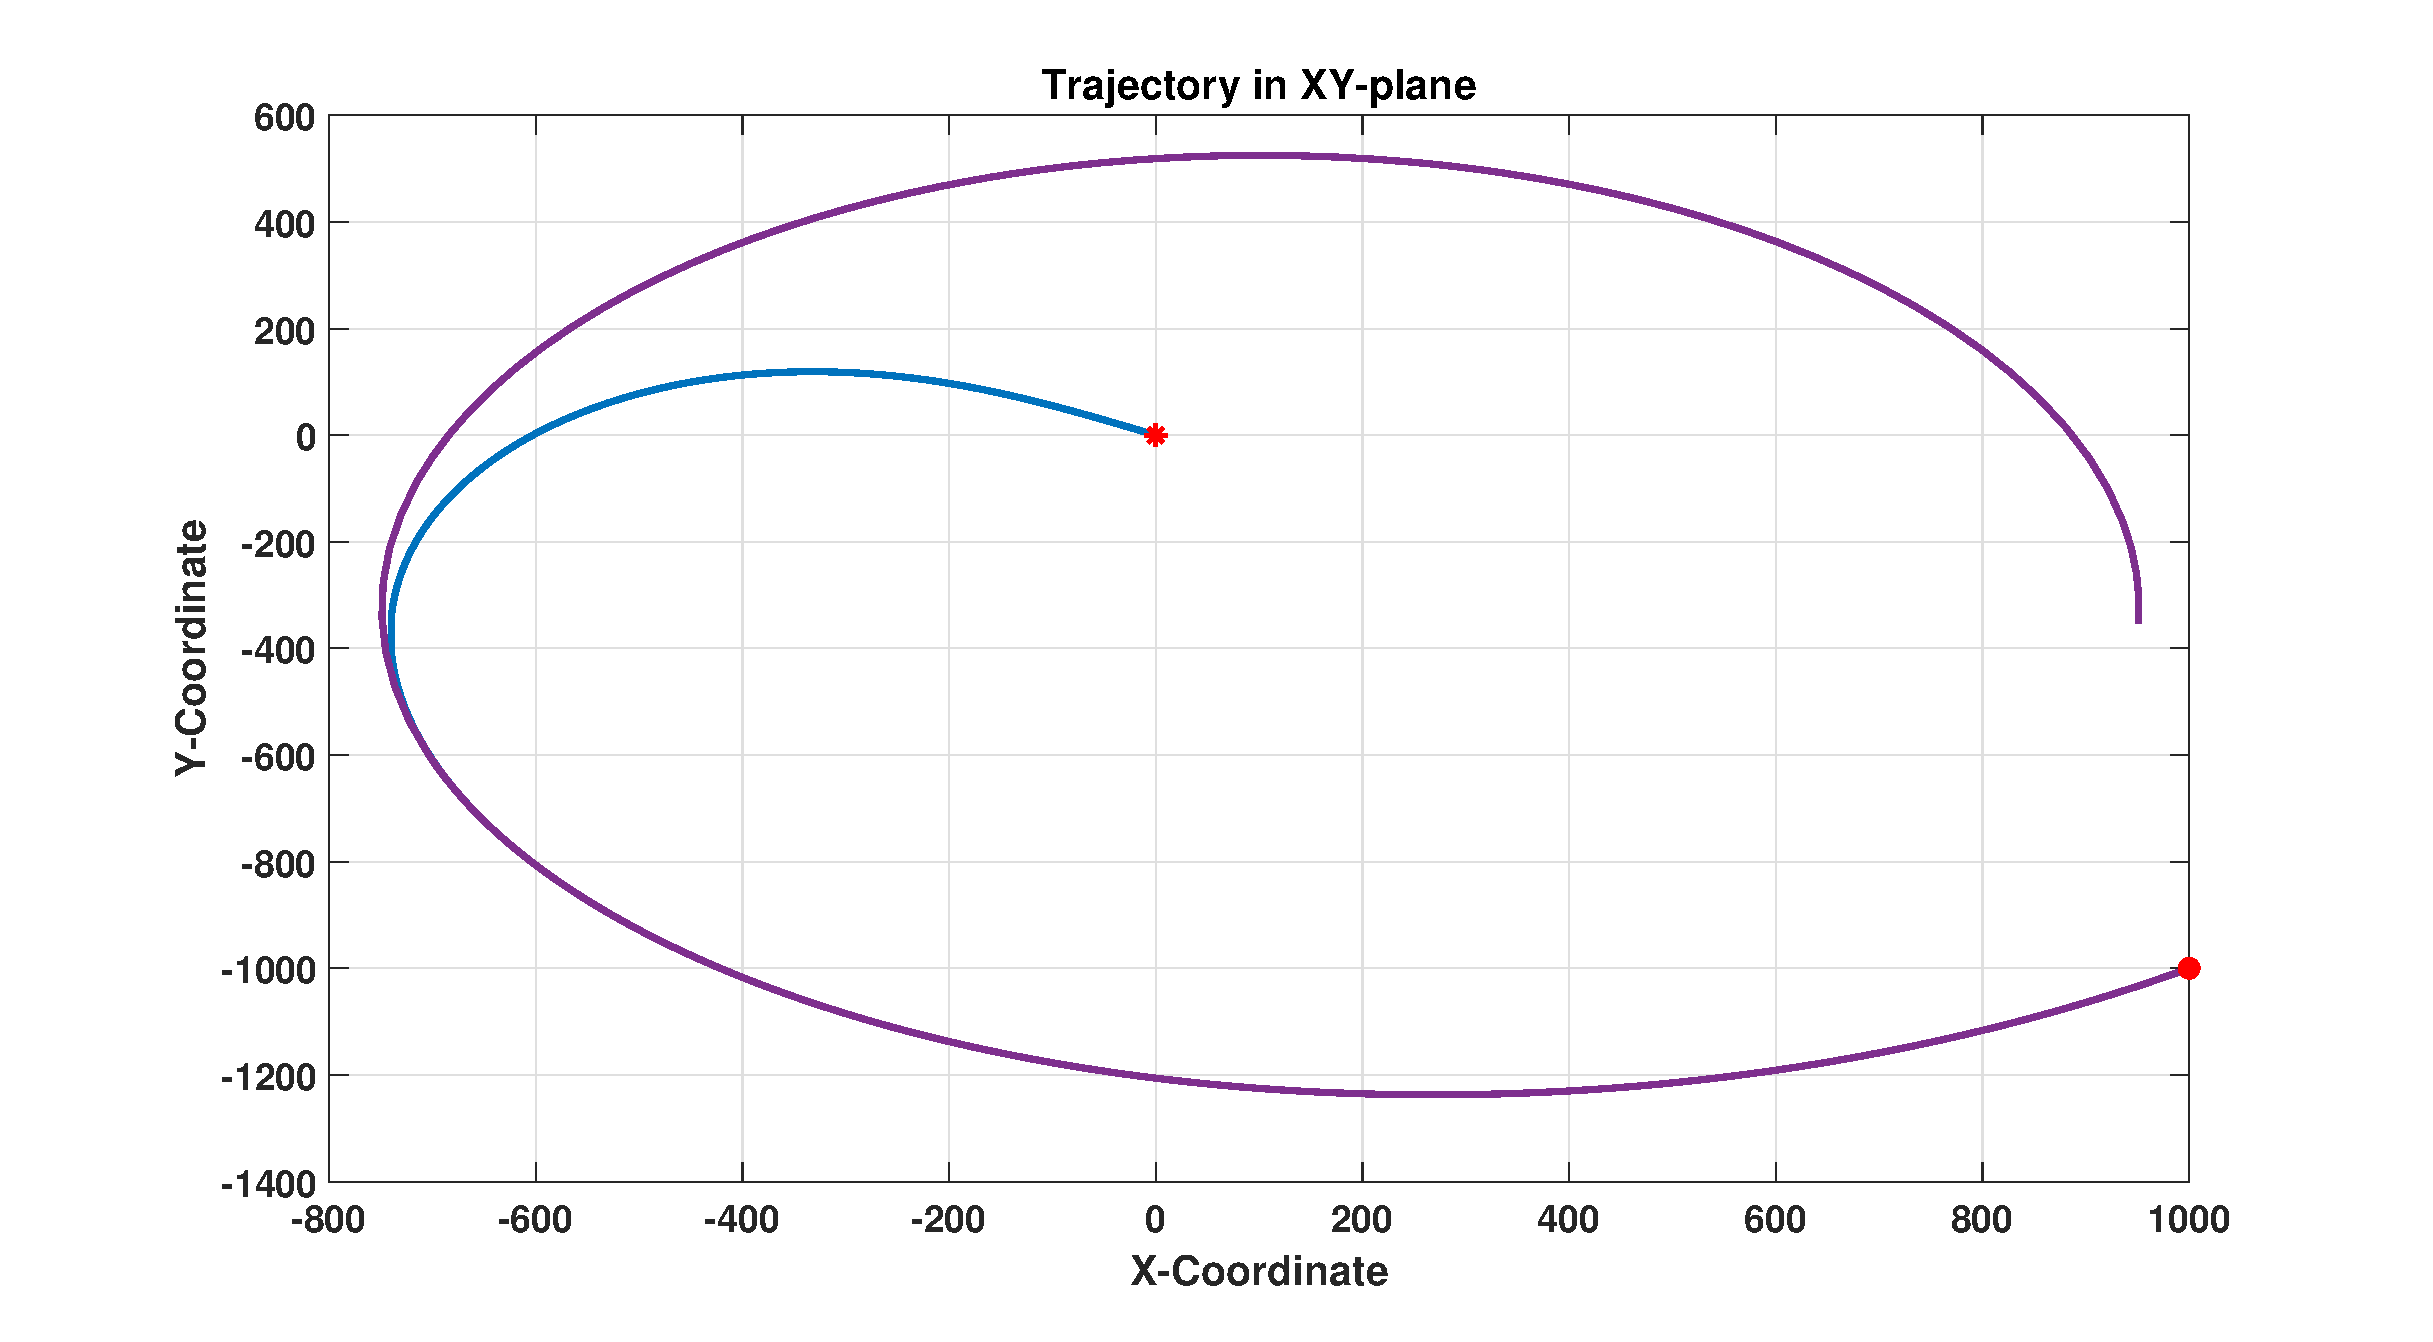
\includegraphics[scale=0.2]{Images/Trajectory_Kushagra.eps}
			\end{figure}
		\end{column}
		\begin{column}{0.5\textwidth}
			\begin{figure}
				\centering
				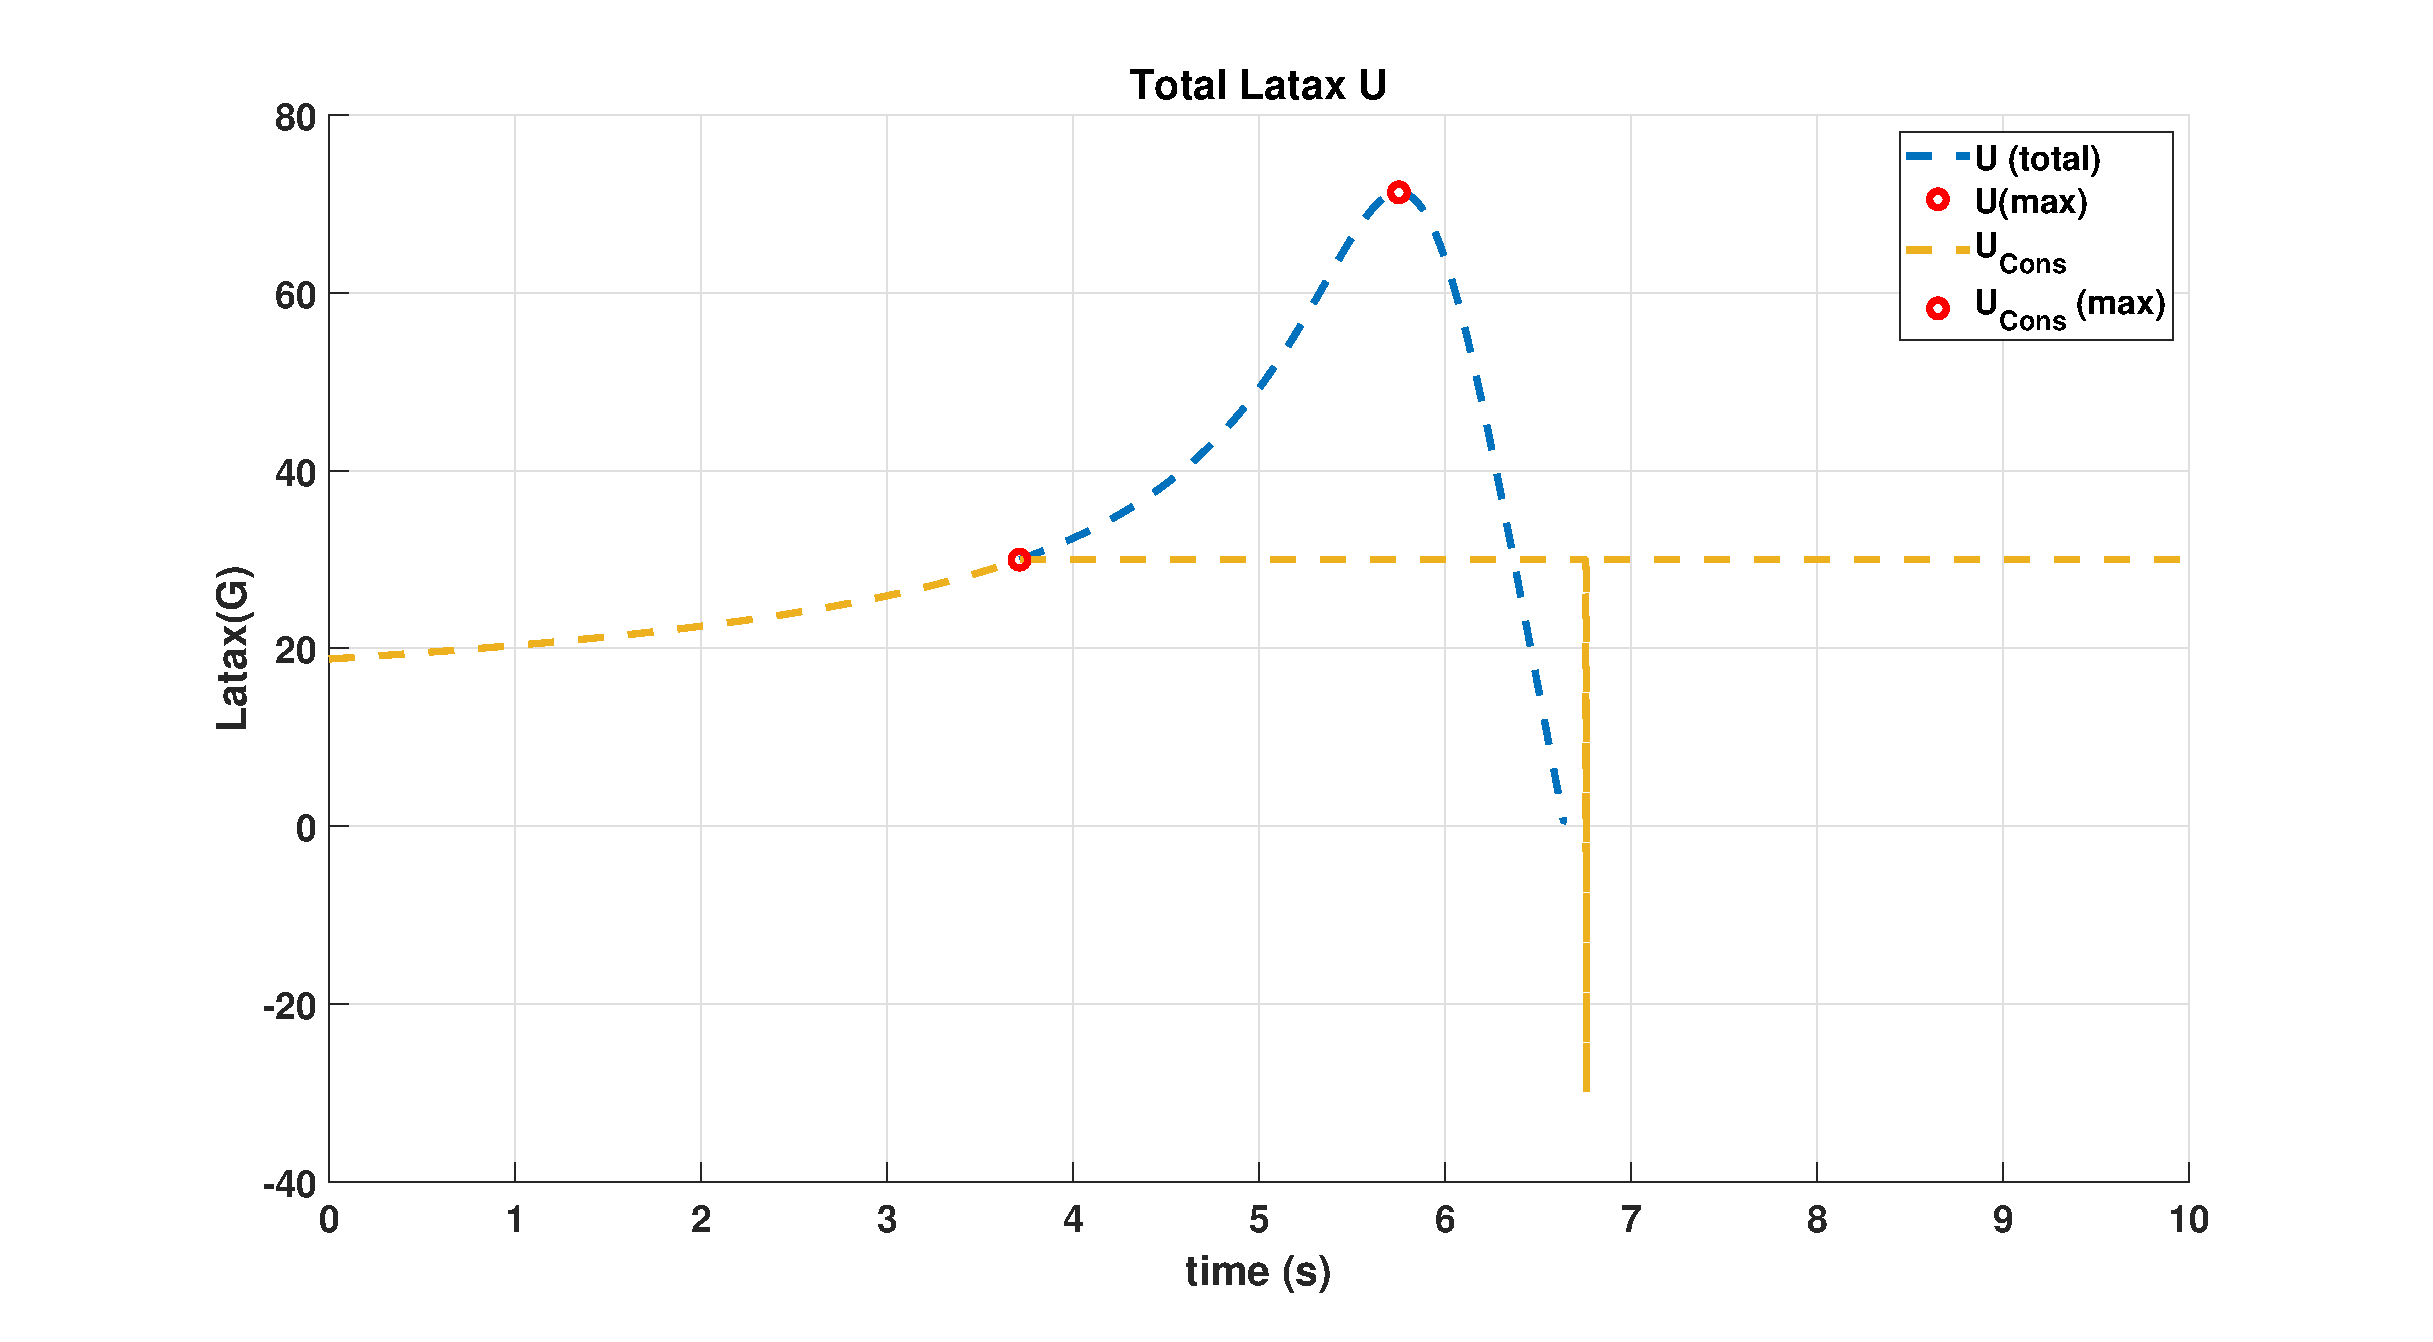
\includegraphics[scale=0.2]{Images/Latax_Kushagra.eps}
			\end{figure}
		\end{column}
	\end{columns}
\footnotetext[1]{\textcolor{blue}{Mishra, K., Mukherjee, D., \& Kumar, S. R. (2024, July). Spiral-based Guidance Strategy for Interception of Stationary Targets. In 2024 American Control Conference (ACC) (pp. 797-802). IEEE.}}
\end{frame}
%%%%%%%%%%%%%%%%%%%%%%%%%%%%%%%%%%%%%%%%%%%%%%%%%%%%%
\begin{frame}
		\begin{block}{Advantages of Spiral Based Trajectories}
		\begin{itemize}
			\item Direct Impact Angle Control : The geometry of the spiral is directly linked to the final impact angle.
			\item Curvature Constrained Path : Latax required by the pursuer throughout the engagement remains bounded.
			\item Terminal Acceleration : The terminal curvature ($\kappa$) and thus the terminal acceleration ($a$) tends to zero as $\lambda \rightarrow \zeta$.  
		\end{itemize}
	\end{block}
	\begin{myblock}{Two Stage Adaptive Law}
		We propose to use a geometric rule based on generalized spirals, $r(\alpha,\lambda) = \alpha (\lambda - \zeta)^\beta$.
		
		We introduce a two-stage Adaptive Control Technique to achieve the desired impact angle with the constrained Latax. 
		
		\textbf{Phase 1:} Feasibility Seeking : Calculate $\alpha_{ref} = \frac{v_p^2f(\beta)}{a_{max}}$. If $\alpha_0 < \alpha_{ref}$, then, drive the $\alpha$ to $\alpha_{ref}$. Otherwise, proceed directly with phase 2.\\
		\vspace{0.2cm}
		\textbf{Phase 2:} Terminal Guidance : We make $\dot{\alpha}=0$. Phase 1 already ensured that Constrained Latax is sufficient to drive the pursuer to the target.
	\end{myblock}
\end{frame}
%%%%%%%%%%%%%%%%%%%%%%%%%%%%%%%%%%%%%%%%%%%%%%%%%%%%%
\begin{frame}{Guidance Law for Phase 1}
\begin{myblock}{Feasibility Seeking}
	Given the dynamics of the system as follows:
	$$\begin{bmatrix}
		\dot{r_p} \\ 
		\dot{\lambda_p} \\
		\dot{\gamma_p}
	\end{bmatrix}=\begin{bmatrix}
	-v_p \cos(\gamma_p-\lambda_p) \\ 
	\frac{-v_p \sin(\gamma_p-\lambda_p)}{r_p} \\
	(a_p+n)/v_p
	\end{bmatrix}=\begin{bmatrix}
	-v_p \cos(\delta_p) \\ 
	\frac{-v_p \sin(\delta_p)}{r_p} \\
	(a_p+n)/v_p
	\end{bmatrix}$$
	where, $\max(n)=N_0$ is assumed to be bounded uniformly distributed noise. We take \\
	$$e=e_{shape}+k_re_{scale}$$
	where, $e_{shape}=\delta_p-\tan^{-1}{(\frac{\lambda_p-\zeta}{\beta}}), ~~ e_{scale}= r-\alpha(\lambda_p-\zeta)^{\beta}$.
\end{myblock}
\end{frame}
%%%%%%%%%%%%%%%%%%%%%%%%%%%%%%%%%%%%%%%%%%%%%%%%%%%%%
\begin{frame}
%	\begin{myblock}{}
		$$\boxed{\dot{e} = \dot{e}_{shape}+k_r\dot{e}_{scale}}$$
		$\mathbf{\dot{e}_{shape}}=\frac{a_p+n}{v_p}+\frac{v_p\sin(\delta_p)}{r_p}(1+\frac{1}{\beta(1+(\lambda_p-\zeta)^2/\beta^2)}),\quad \mathbf{\dot{e}_{scale}}=-v_p\cos(\delta_p)+\frac{v_p\sin(\delta_p)\alpha\beta(\lambda_p-\zeta)^{\beta-1}}{r_p}-\dot{\alpha}(\lambda_p-\zeta)^\beta$
		
		\vspace{0.2cm}
		Choosing,
		\begin{align*}
		a_{p} =& \color{magenta}{\underbrace{-\frac{v_p^2\sin(\delta_p)}{r_p}(1+\frac{1}{\beta(1+(\lambda_p-\zeta)^2/\beta^2)})}_{a_{shape}}}+\color{blue}{\underbrace{k_r(v_p^2\cos(\delta_p)-\frac{v_p^2\sin(\delta_p)\alpha\beta(\lambda_p-\zeta)^{\beta-1}}{r_p}+v_p\dot{\alpha}(\lambda_p-\zeta)^\beta)}_{a_{scale}}}\\
		&\color{teal}{+\underbrace{(\frac{c_1|e|^{\alpha_1}}{\tau^{\mu_1}}+\frac{c_2|e|^{\alpha_2}}{\tau^{\mu_2}})sgn(e)}_{a_{uncertain}}}	
		\end{align*}
		
	where $c_1,c_2,\mu_1,\mu_2 \in \mathbb{R} > 0,~~ \alpha_1 \in (0,1),~~ \alpha_2 > 1, ~~ \tau = T^*-t$
		
%	\end{myblock}
\begin{block}{}
		Appropriate values of the controller parameters and a proportional control for $\dot{\alpha}=K_p(\alpha_{ref}-\alpha(t))$, achieve the feasible trajectory. 
\end{block}
\end{frame}
%%%%%%%%%%%%%%%%%%%%%%%%%%%%%%%%%%%%%%%%%%%%%%%%%%%%%
\begin{frame}{Guidance Law for Phase 2}
	\begin{myblock}{Terminal Guidance}
		We take $\boxed{\dot{\alpha}=0}$ for this phase. Thus, $$\dot{e}_{scale}=-v_p\cos(\delta_p)+\frac{v_p\sin(\delta_p)\alpha\beta(\lambda_p-\zeta)^{\beta-1}}{r_p}$$
		
		Making $\dot{e}_{scale}=0$, 
		$$ \tan \delta_p = \frac{(\lambda - \zeta)}{\beta} \implies e_{shape}=0$$
		Therefore, $e_{scale}$ and $e_{shape}$ converges to the same geometric law as mentioned in the earlier paper\footnotemark[1].
	\end{myblock}
	\footnotetext[1]{\textcolor{blue}{Mishra, K., Mukherjee, D., \& Kumar, S. R. (2024, July). Spiral-based Guidance Strategy for Interception of Stationary Targets. In 2024 American Control Conference (ACC) (pp. 797-802). IEEE.}}
\end{frame}
%%%%%%%%%%%%%%%%%%%%%%%%%%%%%%%%%%%%%%%%%%%%%%%%%%%%%
\begin{frame}{Simulation Parameters}
\begin{itemize}
	\item Pursuer Position: $ x_p(0) = 1000 \text{ m};~~ y_p(0) = -1000 \text{ m}$
	\item Target Position: $x_t(0) = 0 \text{ m};~~y_t(0) = 0 \text{ m}$
	\item Pursuer's Constant Velocity: $v_p = 500 \text{ m/s}$
	\item Lead Angle: $\delta_p(0) = \pi/6$
	\item Desired Impact Angle: $\zeta = -\pi/4$
	\item Maximum Acceleration: $a_{max} = 30*9.8 \text{ m/$s^2$}= 30G \text{ m/$s^2$}$
	\item Fixed Spiral Parameter : $\beta = 0.5$
	\item Initial Spiral Parameter : $r_p(0) = 1414.2 \text{ m}, ~~ \alpha(0)=797.8846, ~~ \lambda(0)= 3 \pi/4$
\end{itemize}
	
\end{frame}
%%%%%%%%%%%%%%%%%%%%%%%%%%%%%%%%%%%%%%%%%%%%%%%%%%%%%
\begin{frame}{Trajectory Vs Time}
	%\vspace{-1.0cm}
	\begin{figure}
		\centering
		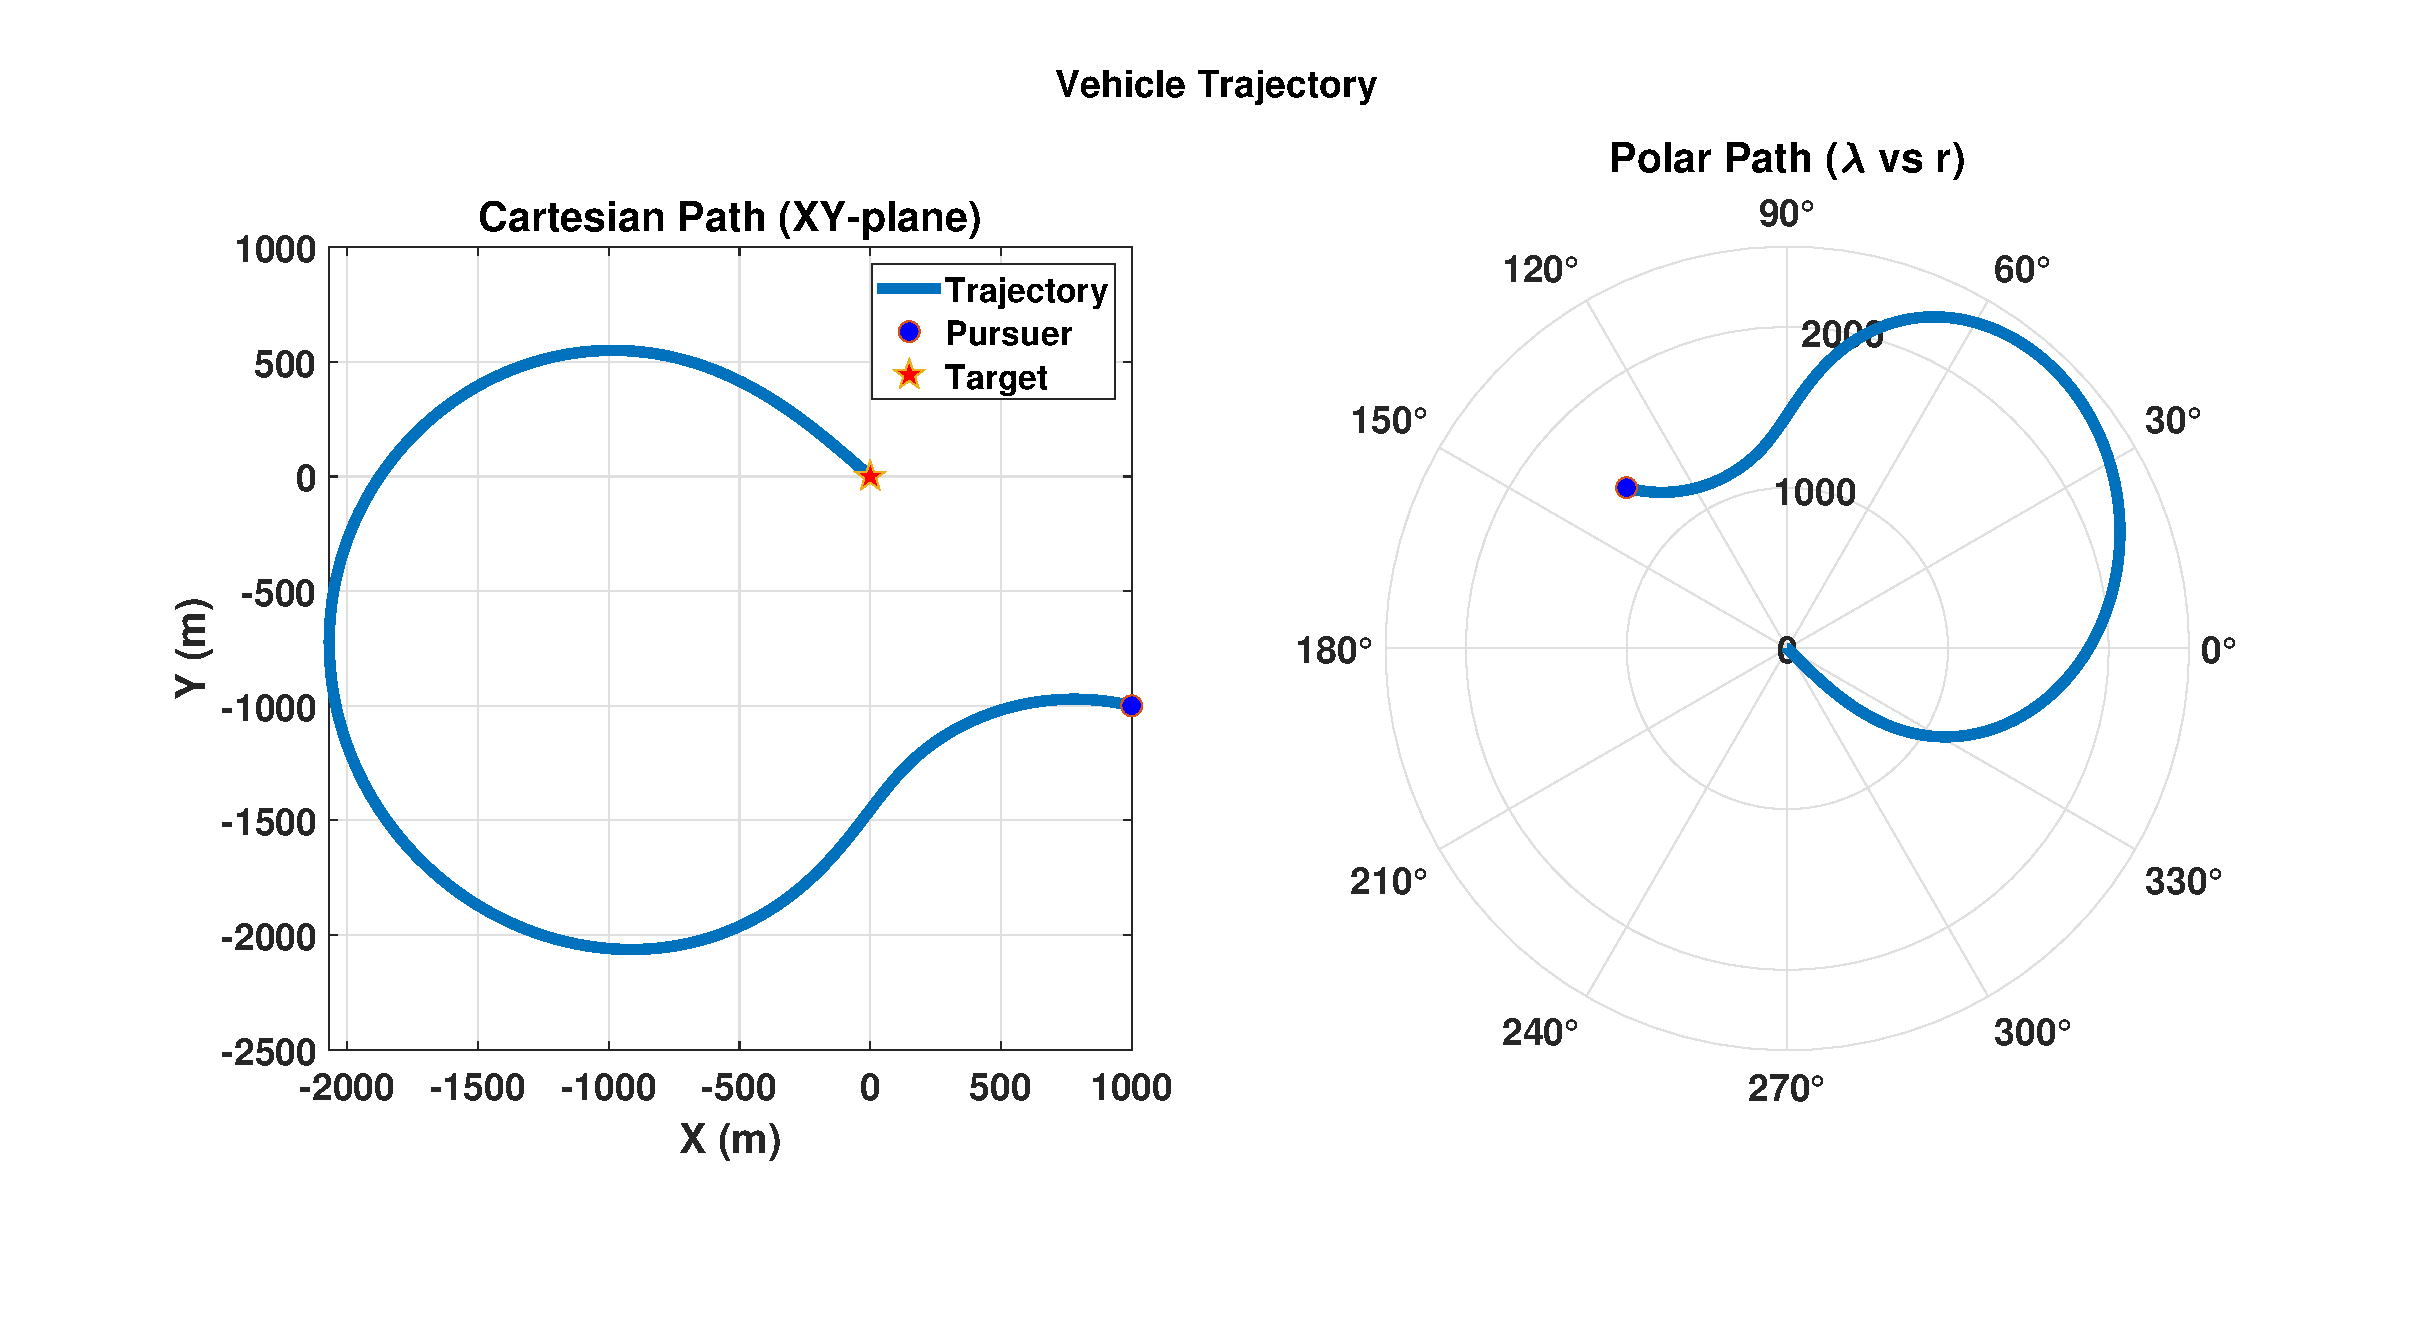
\includegraphics[scale=0.35]{Images/VehicleTrajectory.eps}
	\end{figure}
\end{frame}
%%%%%%%%%%%%%%%%%%%%%%%%%%%%%%%%%%%%%%%%%%%%%%%%%%%%%
\begin{frame}{States vs Time}
	\vspace{-0.3cm}
	\begin{figure}
		\centering
		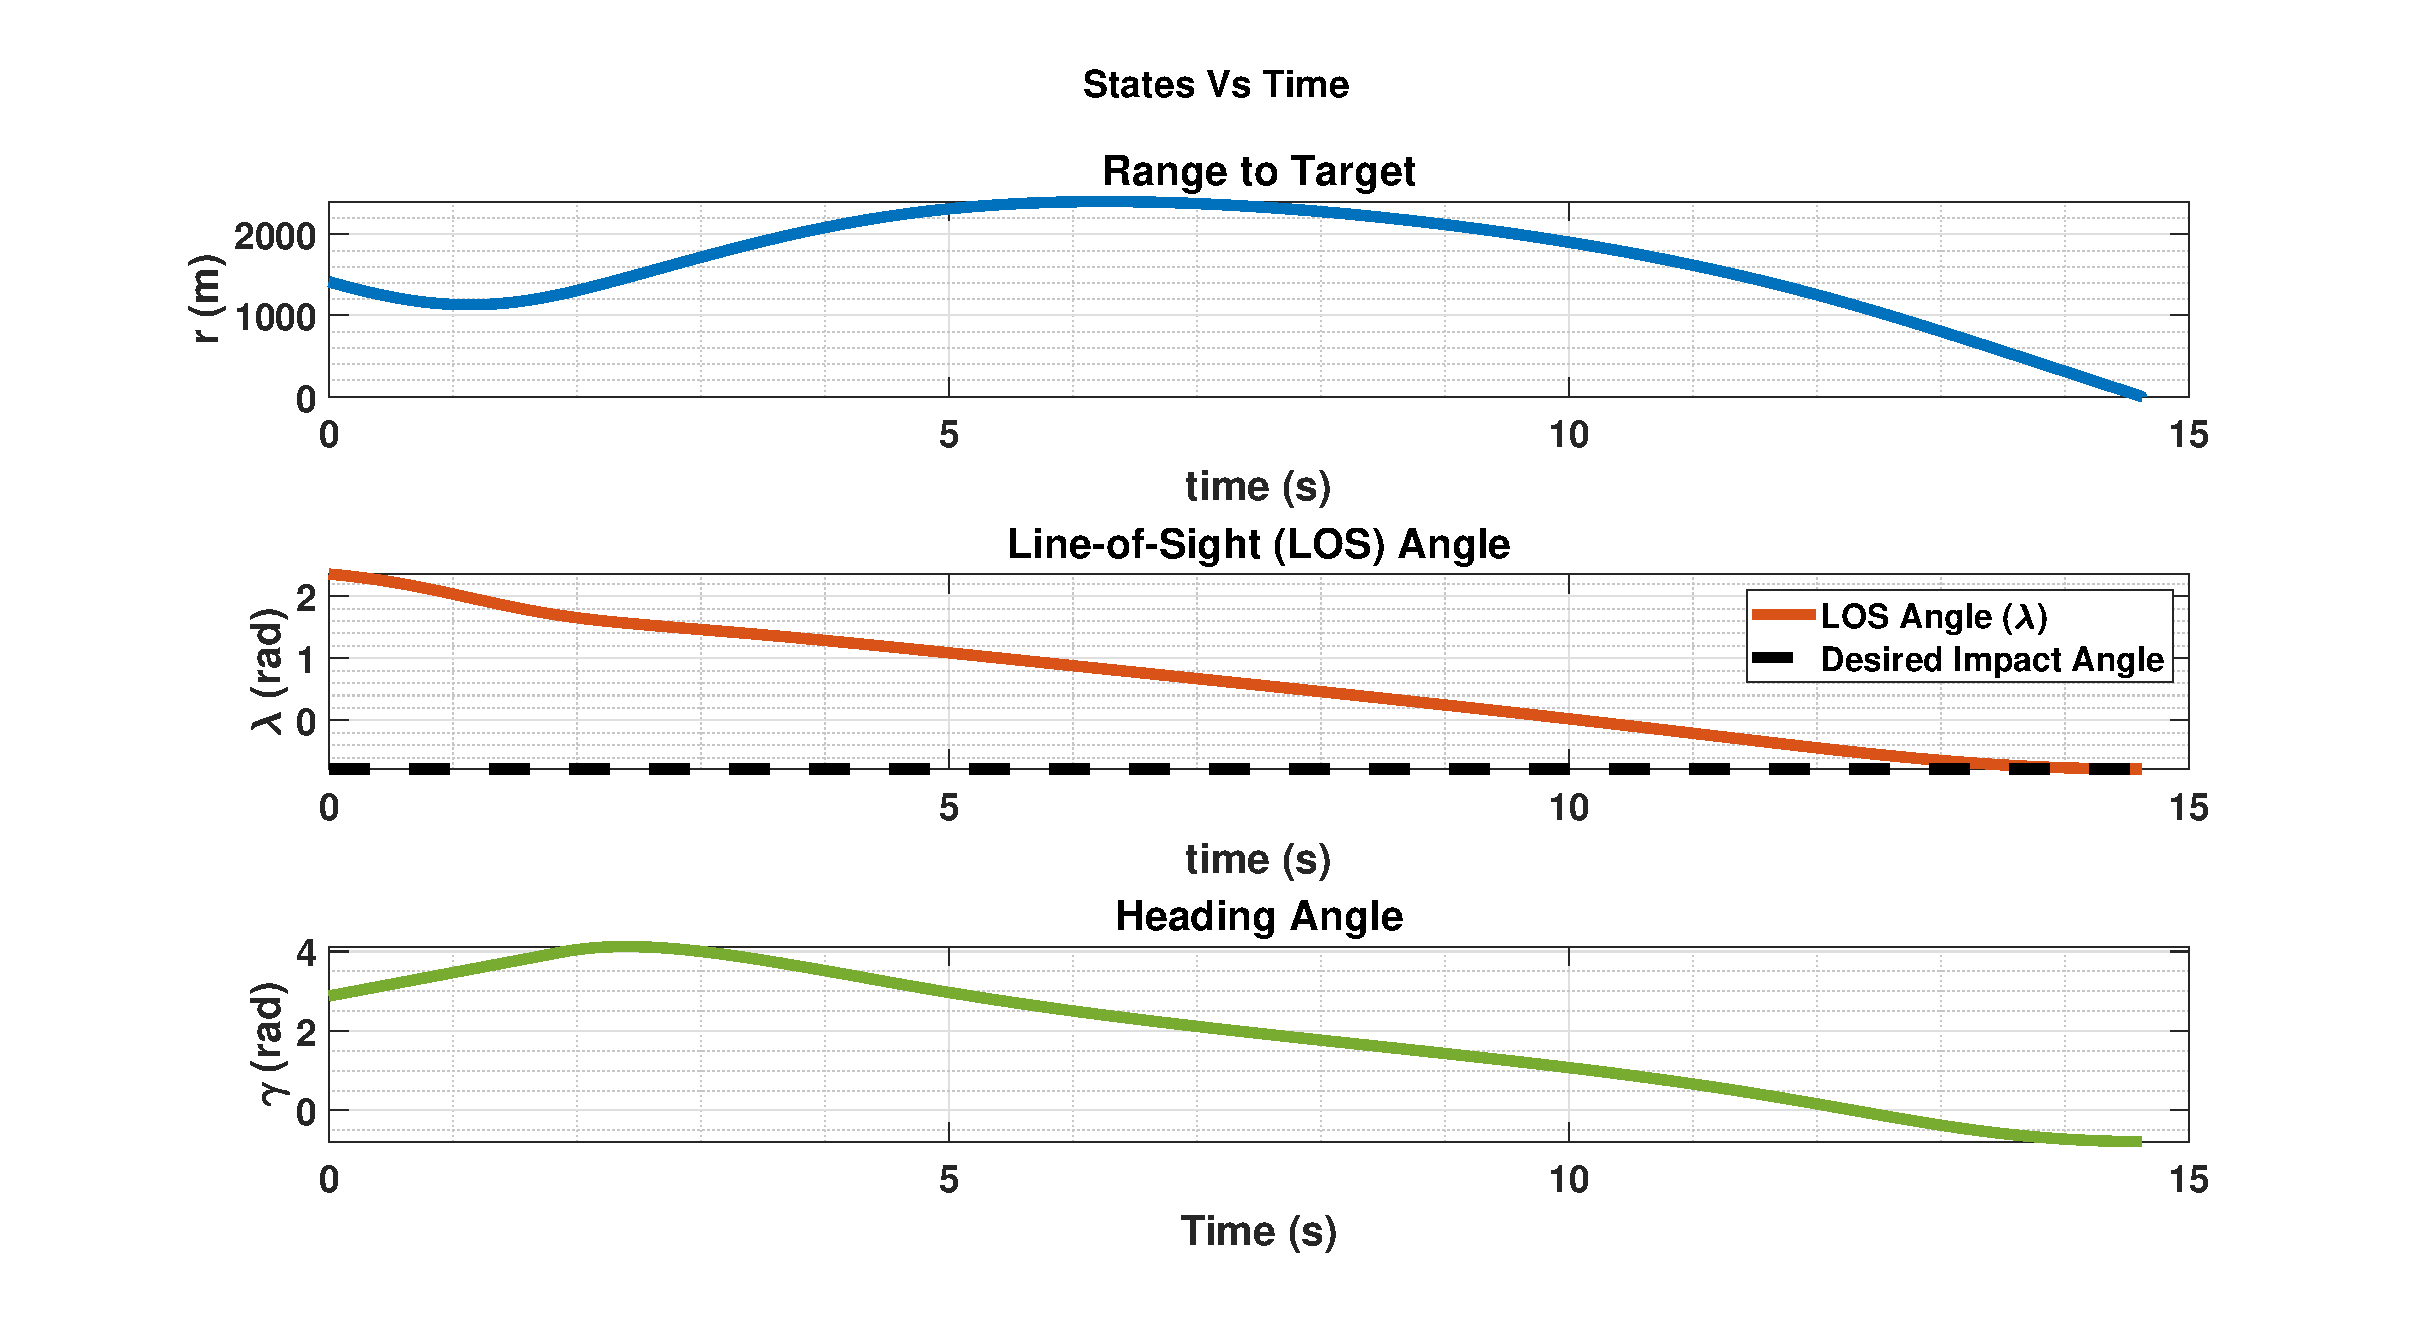
\includegraphics[scale=0.35]{Images/StatesVsTime.eps}
	\end{figure}
\end{frame}
%%%%%%%%%%%%%%%%%%%%%%%%%%%%%%%%%%%%%%%%%%%%%%%%%%%%%
\begin{frame}{Latax Commanded vs Actual}
	\vspace{-0.3cm}
		\begin{figure}
		\centering
		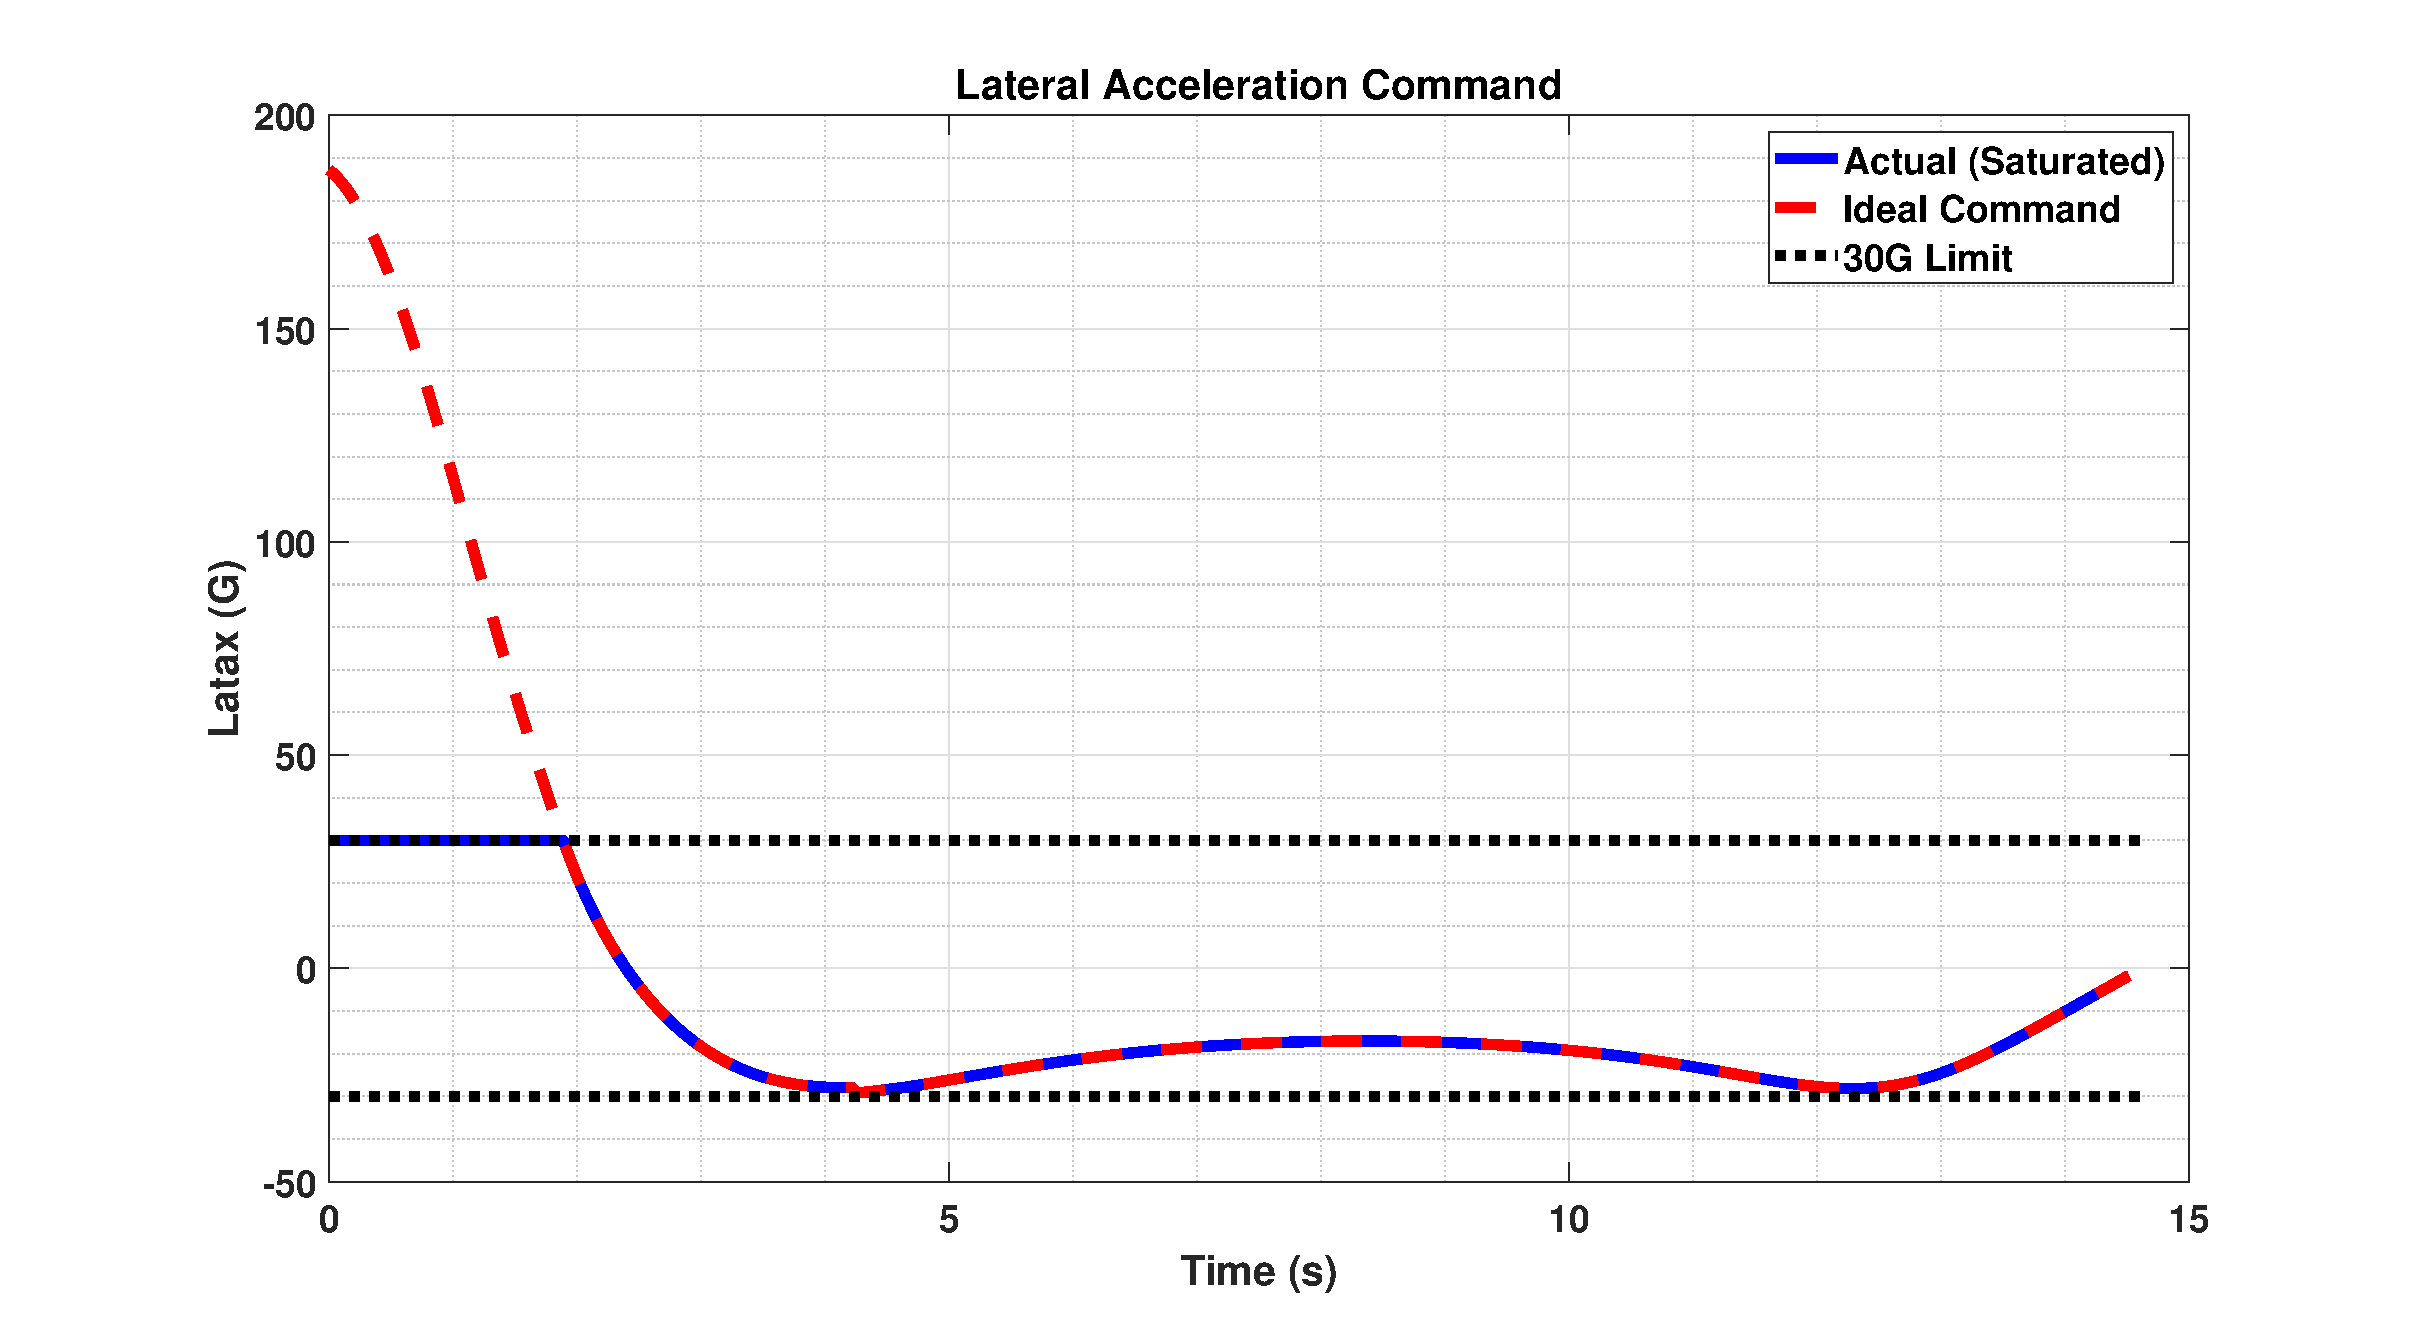
\includegraphics[scale=0.3]{Images/LATAX_ActualVsIdeal.eps}
	\end{figure}
\end{frame}
%%%%%%%%%%%%%%%%%%%%%%%%%%%%%%%%%%%%%%%%%%%%%%%%%%%%%
\begin{frame}{Shape and Scale Input}\label{Control}
	\vspace{-0.3cm}
		\begin{figure}
		\centering
		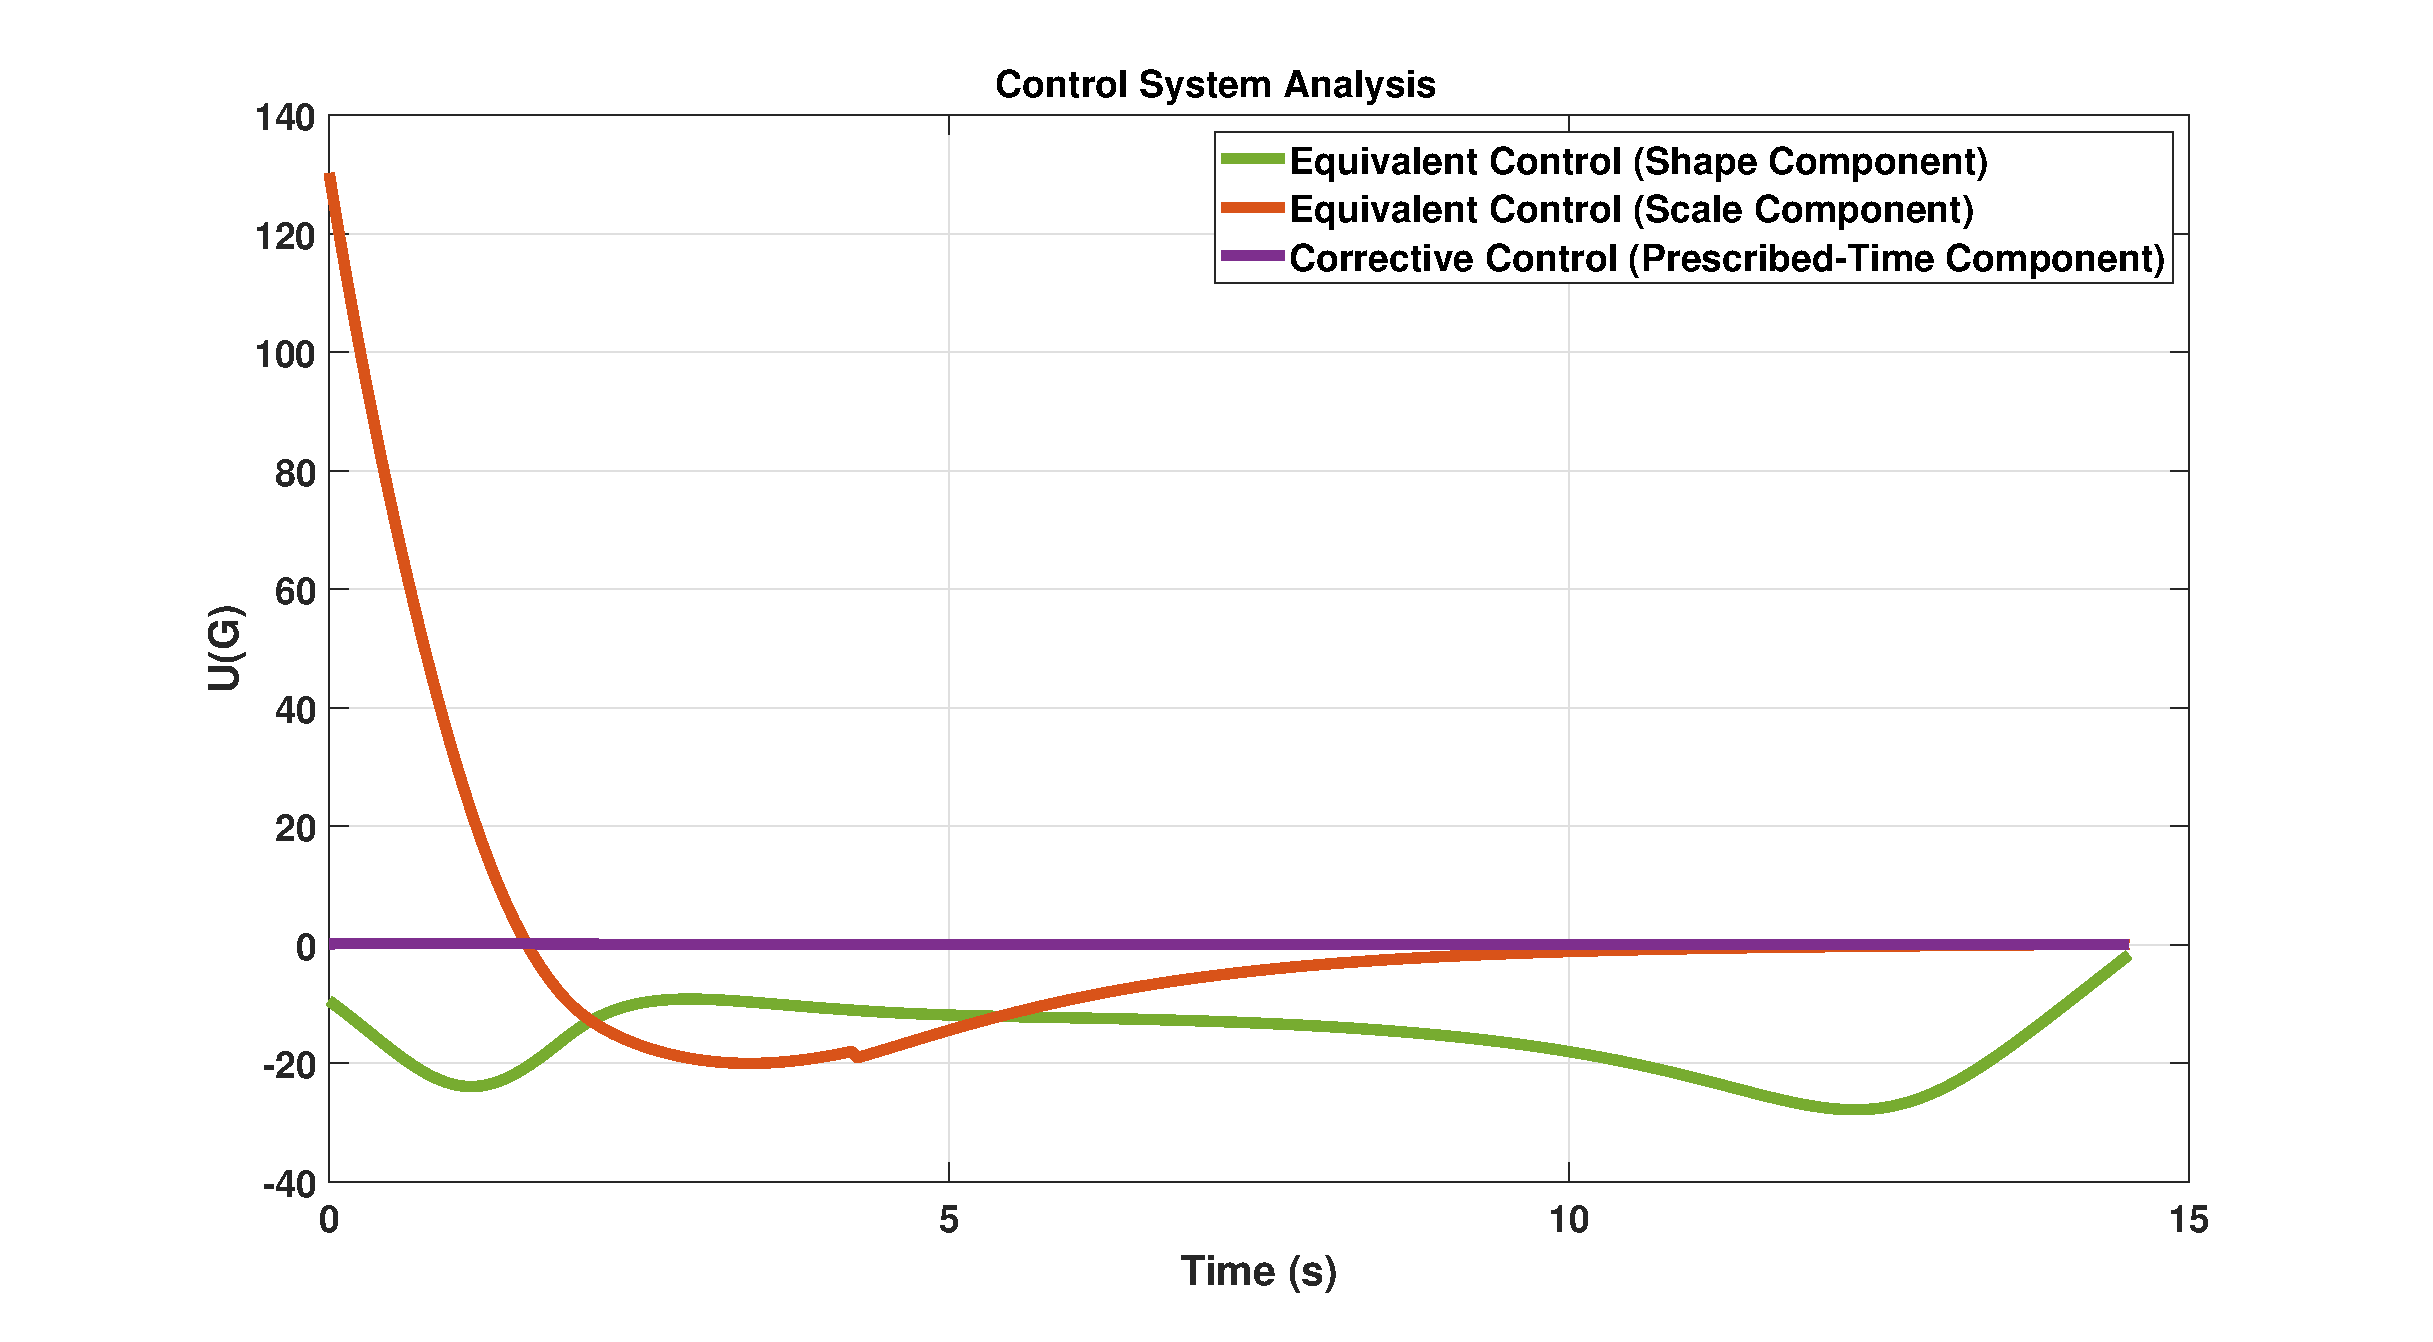
\includegraphics[scale=0.3]{Images/Control_Shape_Scale_PT.eps}
	\end{figure}
	\hyperlink{Corr}{\beamerbutton{PT Control}}
\end{frame}
%%%%%%%%%%%%%%%%%%%%%%%%%%%%%%%%%%%%%%%%%%%%%%%%%%%%%
\begin{frame}{Multi-Agent Extension}
	\begin{block}{Operational Motivation}
		\begin{itemize}
			\item Attack from a specified \textbf{sector} instead of a single direction.
			\item Make System Scalable
			\item Maintain actuator constraint ($a_{max} = 30G$) for all agents.
		\end{itemize}
	\end{block}
	
	\begin{alertblock}{New Challenges}
		\begin{itemize}
			\item Each agent has different initial condition.
			\item Initial Spiral parameter $\alpha_i$ differs for each agent.
			\item Spiral Parameters and Desired Impact Angle both affect the $\alpha_{req}$ for smoother trajectory.  
		\end{itemize}
	\end{alertblock}
\end{frame}
%%%%%%%%%%%%%%%%%%%%%%%%%%%%%%%%%%%%%%%%%%%%%%%%%%%%%
\begin{frame}{Multi-Agent Engagement Model}
	For $i = 1,2,\dots,N$
	\[
	\dot r_i = -v_p \cos(\delta_i)
	\]
	\[
	\dot \lambda_i = \frac{-v_p \sin(\delta_i)}{r_i}
	\]
	\[
	\dot \gamma_i = \frac{a_i}{v_p}
	\]
	
	\begin{block}{Impact Angle Sector Assignment}
		Impact angles distributed inside a sector:
		
		\[
		\zeta_i \in [\theta_{start},\theta_{end}]
		\]
		
		Uniform assignment:
		
		\[
		\zeta_i = \theta_{start} + \frac{i-1}{N-1}
		(\theta_{end}-\theta_{start})
		\]
	\end{block}
	
\end{frame}
%%%%%%%%%%%%%%%%%%%%%%%%%%%%%%%%%%%%%%%%%%%%%%%%%%%%%
\begin{frame}{Spiral Manifold for Each Agent}
	
	Each agent follows:
	
	\[
	r_i = \alpha_i (\lambda_i - \zeta_i)^{\beta_i}
	\]
	
	\begin{block}{Error Definition}
		\[
		e_i = e_{shape,i} + k_r e_{scale,i}
		\]
		
		\[
		e_{shape,i} = \delta_i - \tan^{-1}\left(\frac{\lambda_i - \zeta_i}{\beta_i}\right)
		\]
		
		\[
		e_{scale,i} = r_i - \alpha_i (\lambda_i - \zeta_i)^{\beta_i}
		\]
	\end{block}
	
	Each agent independently satisfies impact angle constraint.
\end{frame}
%%%%%%%%%%%%%%%%%%%%%%%%%%%%%%%%%%%%%%%%%%%%%%%%%%%%%
%%%%%%%%%%%%%%%%%%%%%%%%%%%%%%%%%%%%%%%%%%%%%%%%%%%%%
\begin{frame}{Two-Phase Multi-Agent Guidance}
We introduce coupling at the level of spiral scaling:

\[
\dot{\alpha}_i = -k_\alpha \sum_{j \in \mathcal{N}_i}
(\alpha_i - \alpha_j)
\]

\begin{block}{Leader-Follower Implementation}
	Leader:
	\[
	\alpha_1 \rightarrow \max(\alpha_{min,i})
	\]
	
	Followers:
	\[
	\dot{\alpha}_i = -k_\alpha (\alpha_i - \alpha_{parent})
	\]
\end{block}
	\begin{block}{Phase 1: Feasibility + Consensus}
		\begin{itemize}
			\item Compute $\alpha_{min,i}$
			\item Drive $\alpha_i \rightarrow \alpha_{ref}$
			%\item Apply prescribed-time control on $e_i$
			\item Maintain $|a_i| \le a_{max}$
		\end{itemize}
	\end{block}
\end{frame}
\begin{frame}	
	\begin{block}{Phase 2: Terminal Guidance}
		\begin{itemize}
			\item Freeze $\alpha_i$
			\item Enforce spiral manifold
			\item $\tan \delta_i = \frac{\lambda_i - \zeta_i}{\beta_i}$
			\item Terminal curvature $\rightarrow 0$
		\end{itemize}
	\end{block}
		Ensures:
	\begin{itemize}
		\item Topology is defined in a manner such that it is agnostic to link failures.
		\item Feasible curvature for all agents
		\item Coordinated spiral expansion
		\item Smooth scaling 
	\end{itemize}
\end{frame}
%%%%%%%%%%%%%%%%%%%%%%%%%%%%%%%%%%%%%%%%%%%%%%%%%%%%% 
\begin{frame}{Simulations}	
		N=4; x0 = [1000 1200 800 900]; y0 = [-1000 -900 -1100 -950];\\
		\begin{columns}
			\begin{column}{0.5\textwidth}
				\begin{figure}
					%\centering
					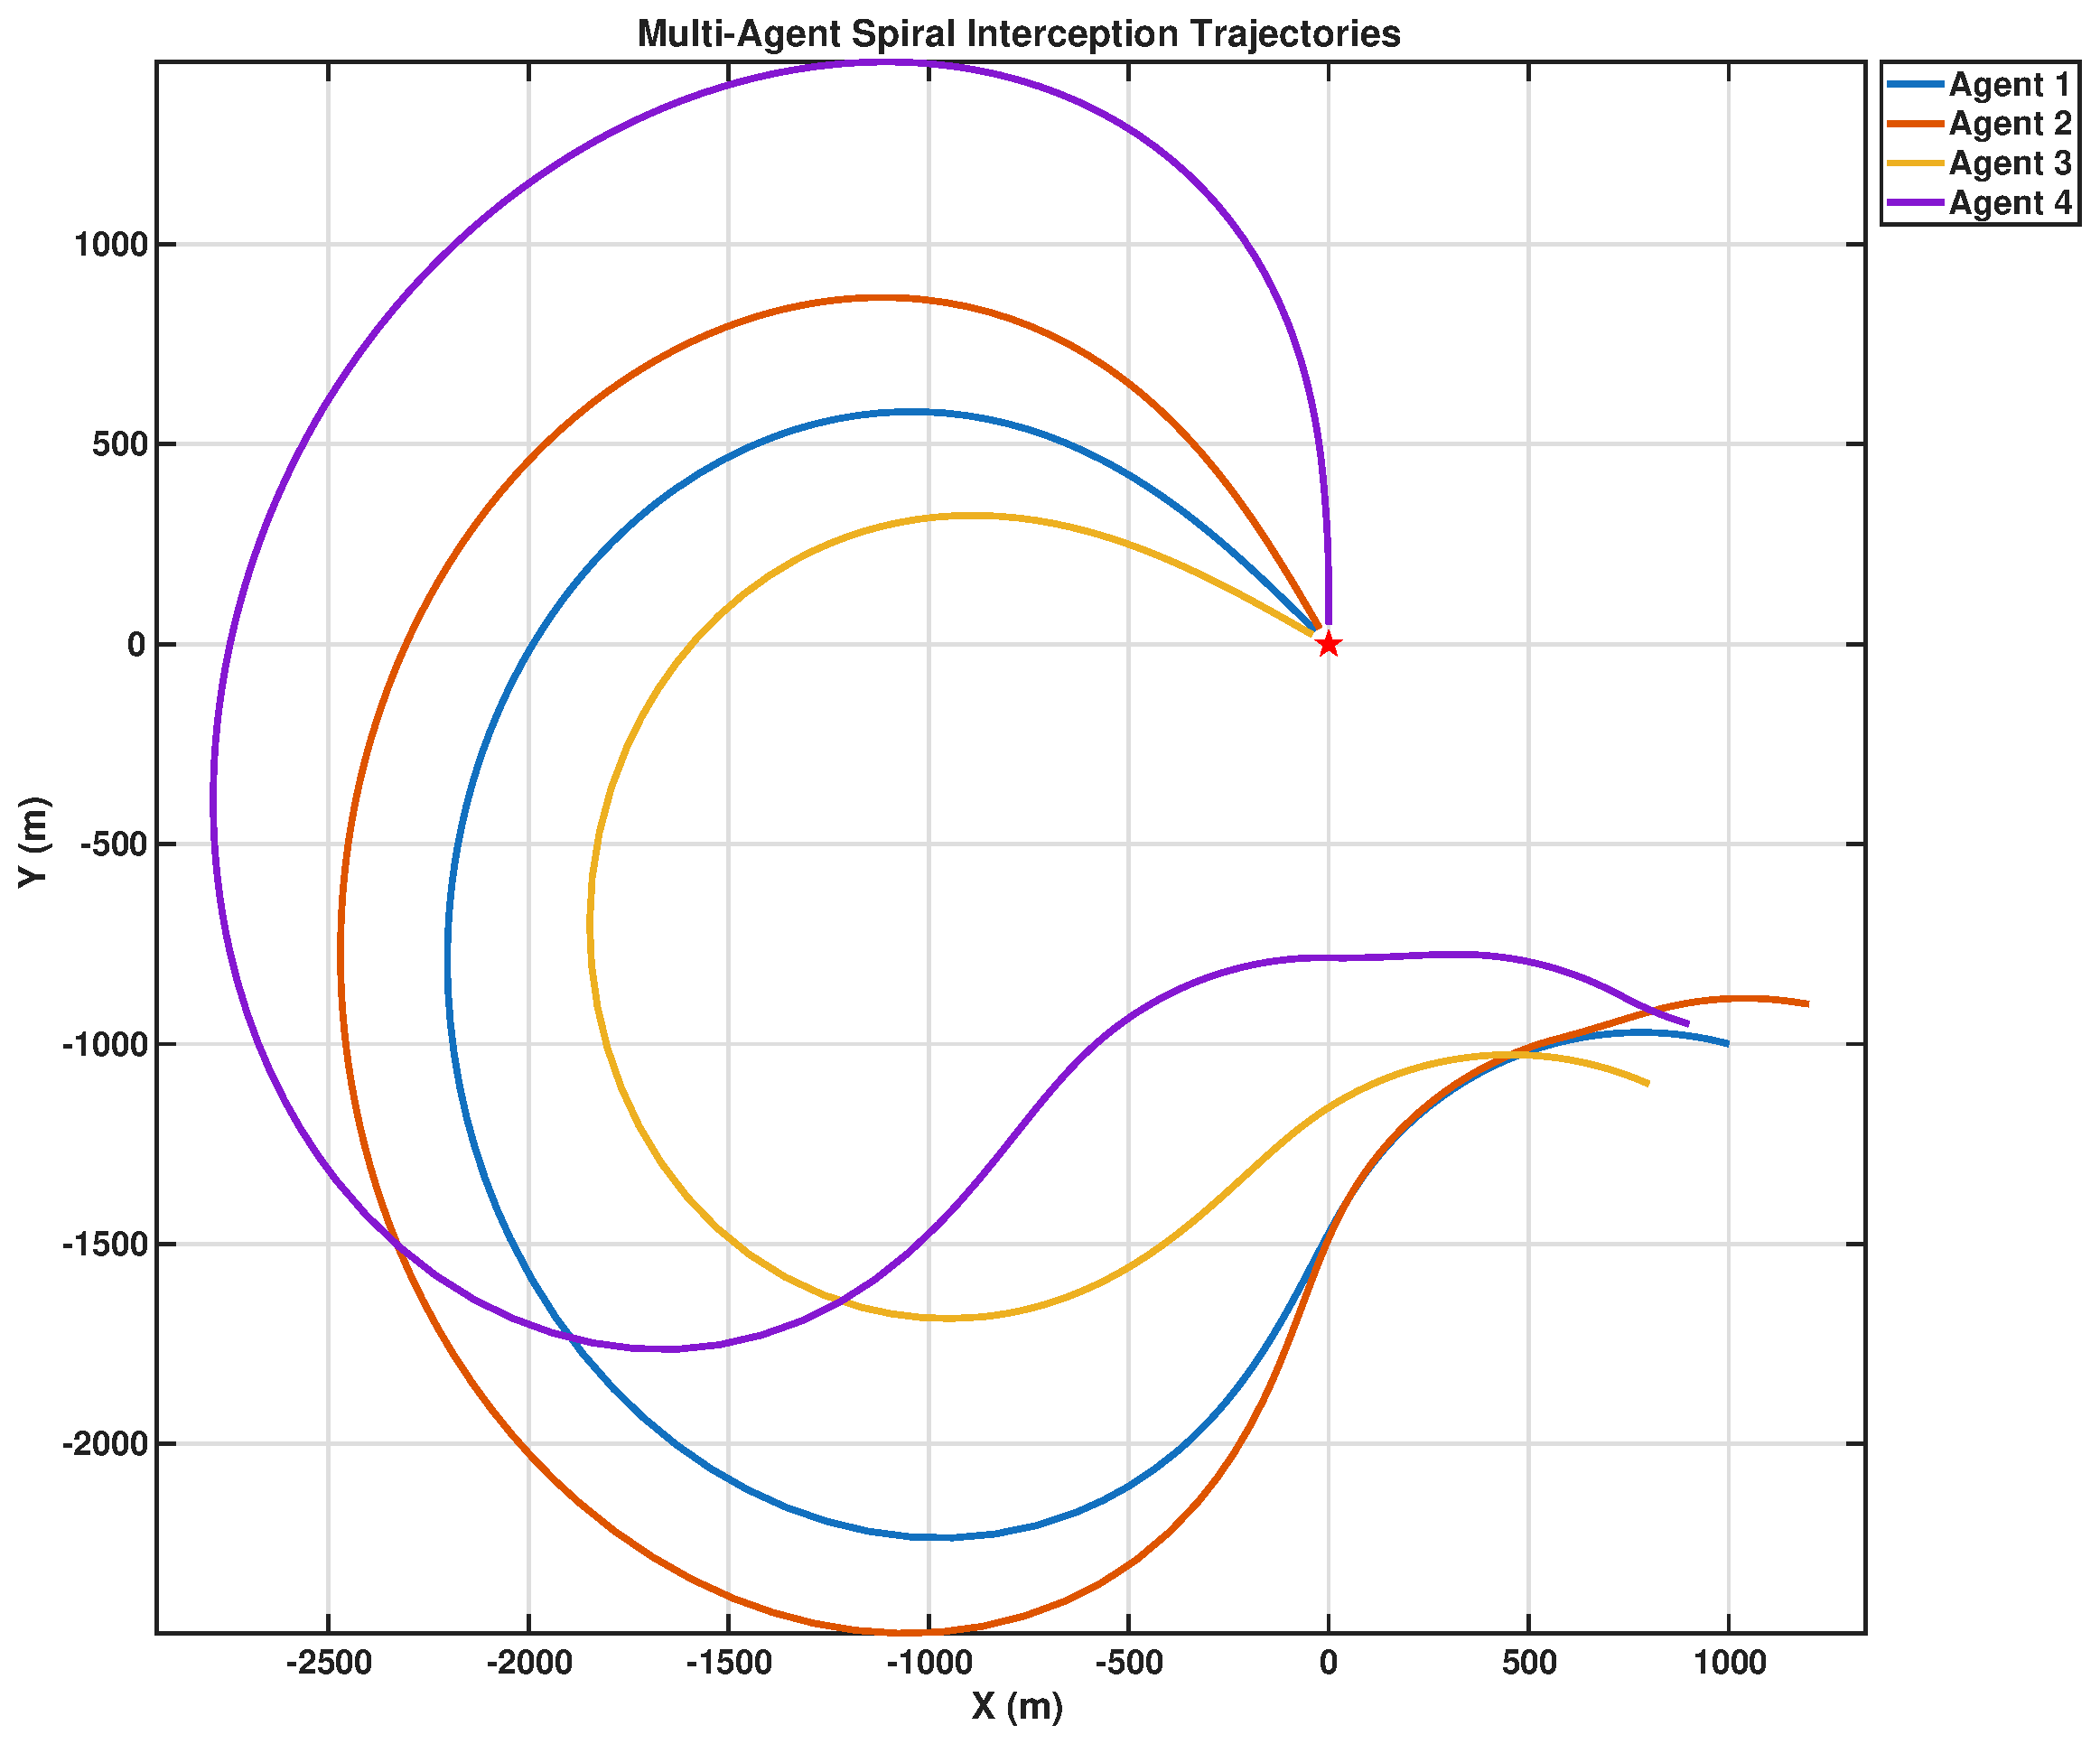
\includegraphics[scale=0.15]{Images/4Agent_Case1_Trajectory.eps}
					\caption{Trajectory of 4 Agents intercepting at different Impact Angle}
				\end{figure}
			\end{column}
			\begin{column}{0.5\textwidth}
				\begin{figure}
					%\centering
					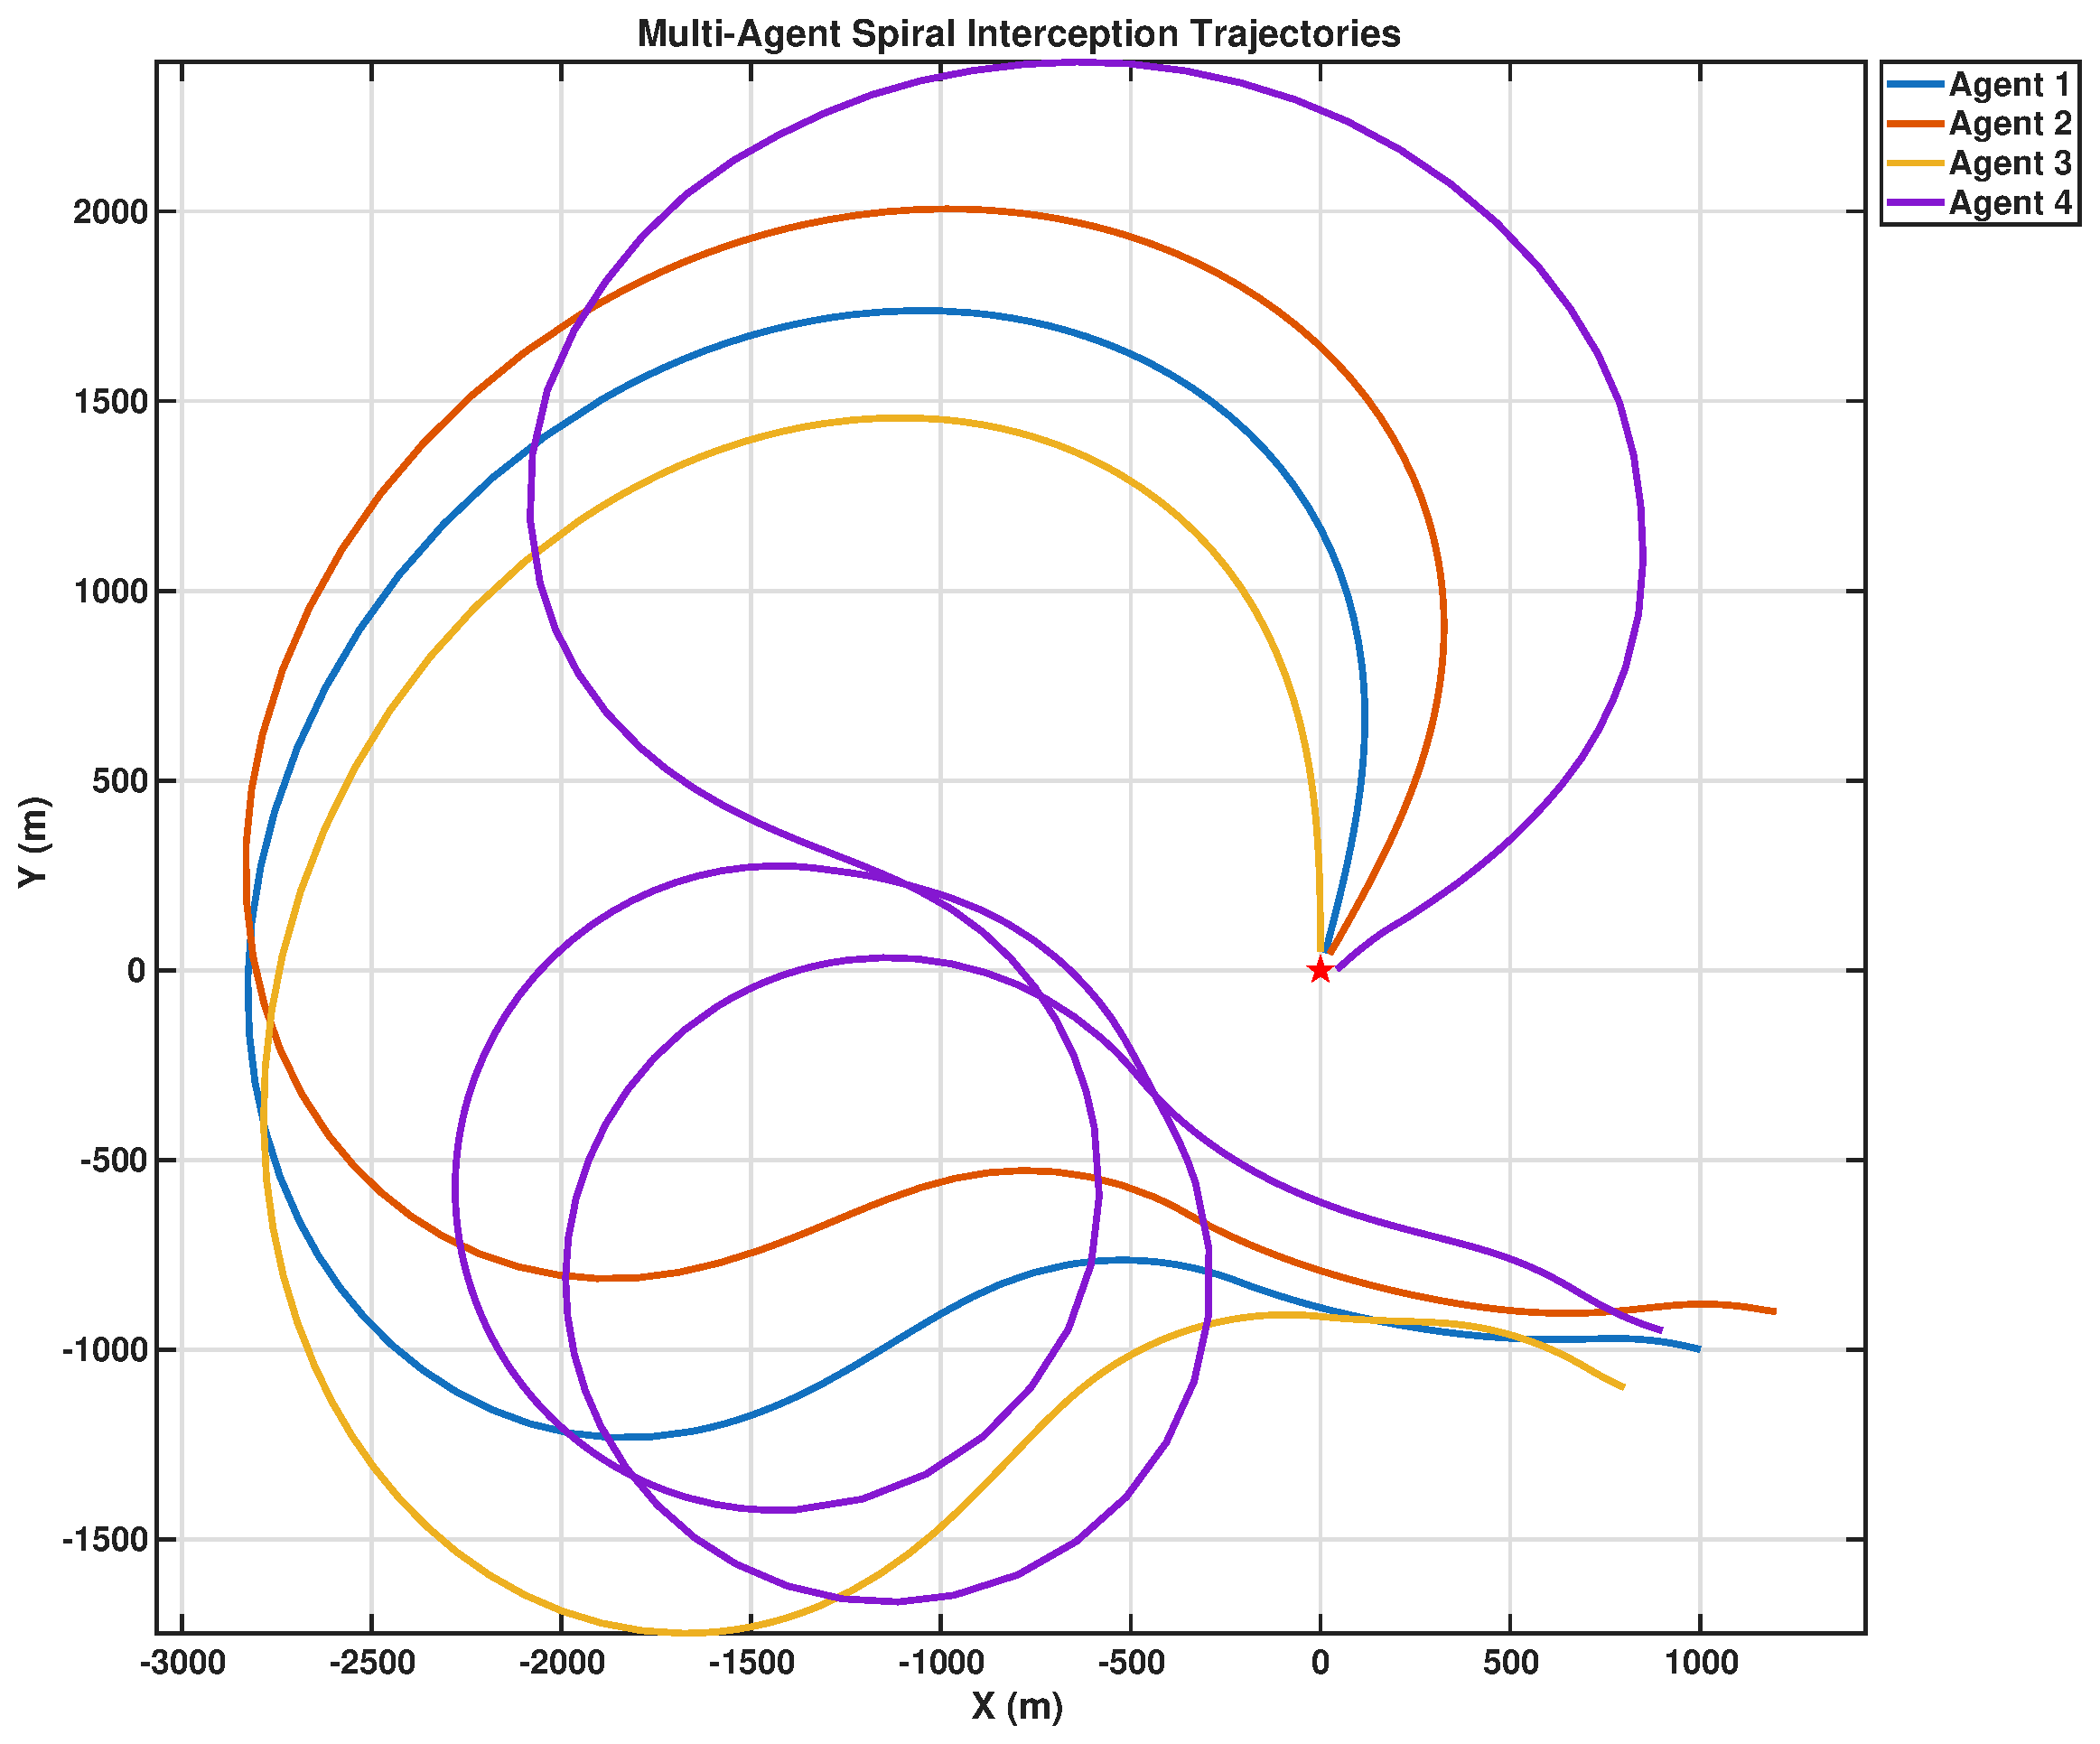
\includegraphics[scale=0.15]{Images/4Agent_Case2_Trajectory.eps}
					\caption{Trajectory of 4 Agents with Impact Angle Sector shifted by $\pi/3$}
				\end{figure}
			\end{column}
		\end{columns}
	
\end{frame}
%%%%%%%%%%%%%%%%%%%%%%%%%%%%%%%%%%%%%%%%%%%%%%%%%%%%% 
\begin{frame}{Simulations}	
	N=4; x0 = [1000 1200 800 900]; y0 = [-1000 -900 -1100 -950];\\
	N=5 x0 = [1000 1200 800 900 1100];y0 = [-1000 -900 -1100 -950 800];
	\begin{columns}
		\begin{column}{0.5\textwidth}
			\begin{figure}
				%\centering
				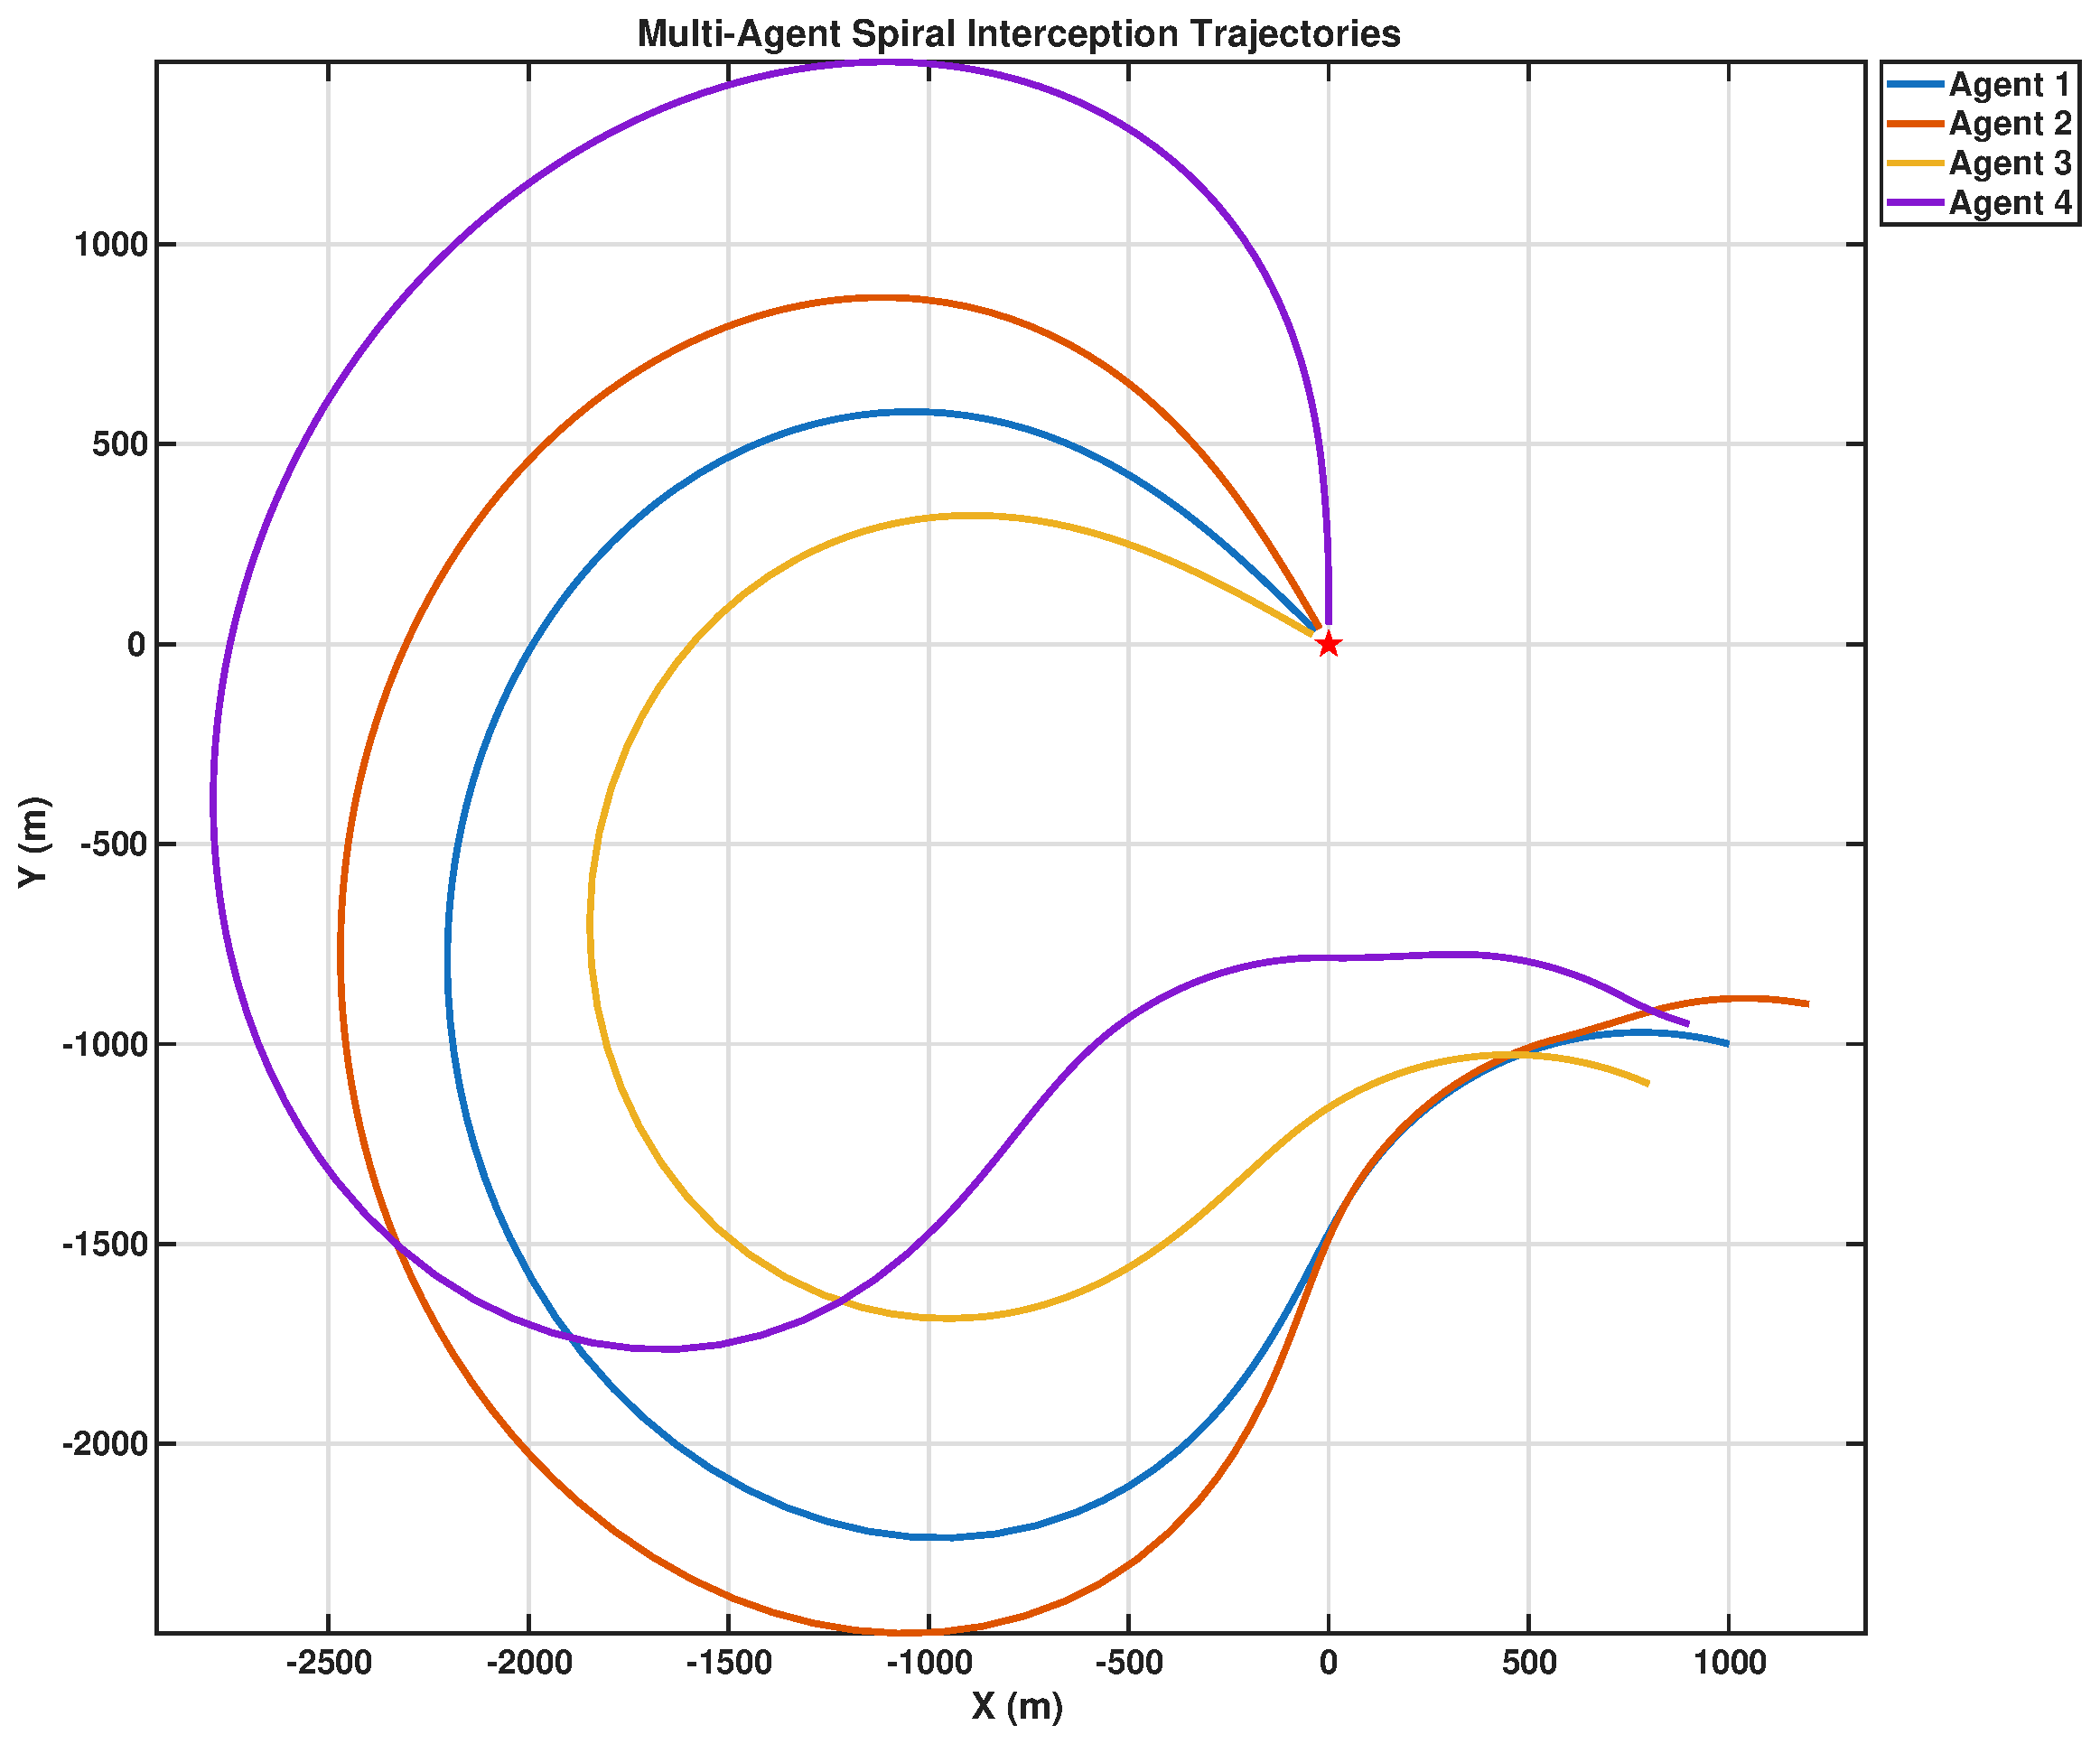
\includegraphics[scale=0.15]{Images/4Agent_Case1_Trajectory.eps}
				\caption{Trajectory of 4 Agents intercepting at different Impact Angle}
			\end{figure}
		\end{column}
		\begin{column}{0.5\textwidth}
			\begin{figure}
				%\centering
				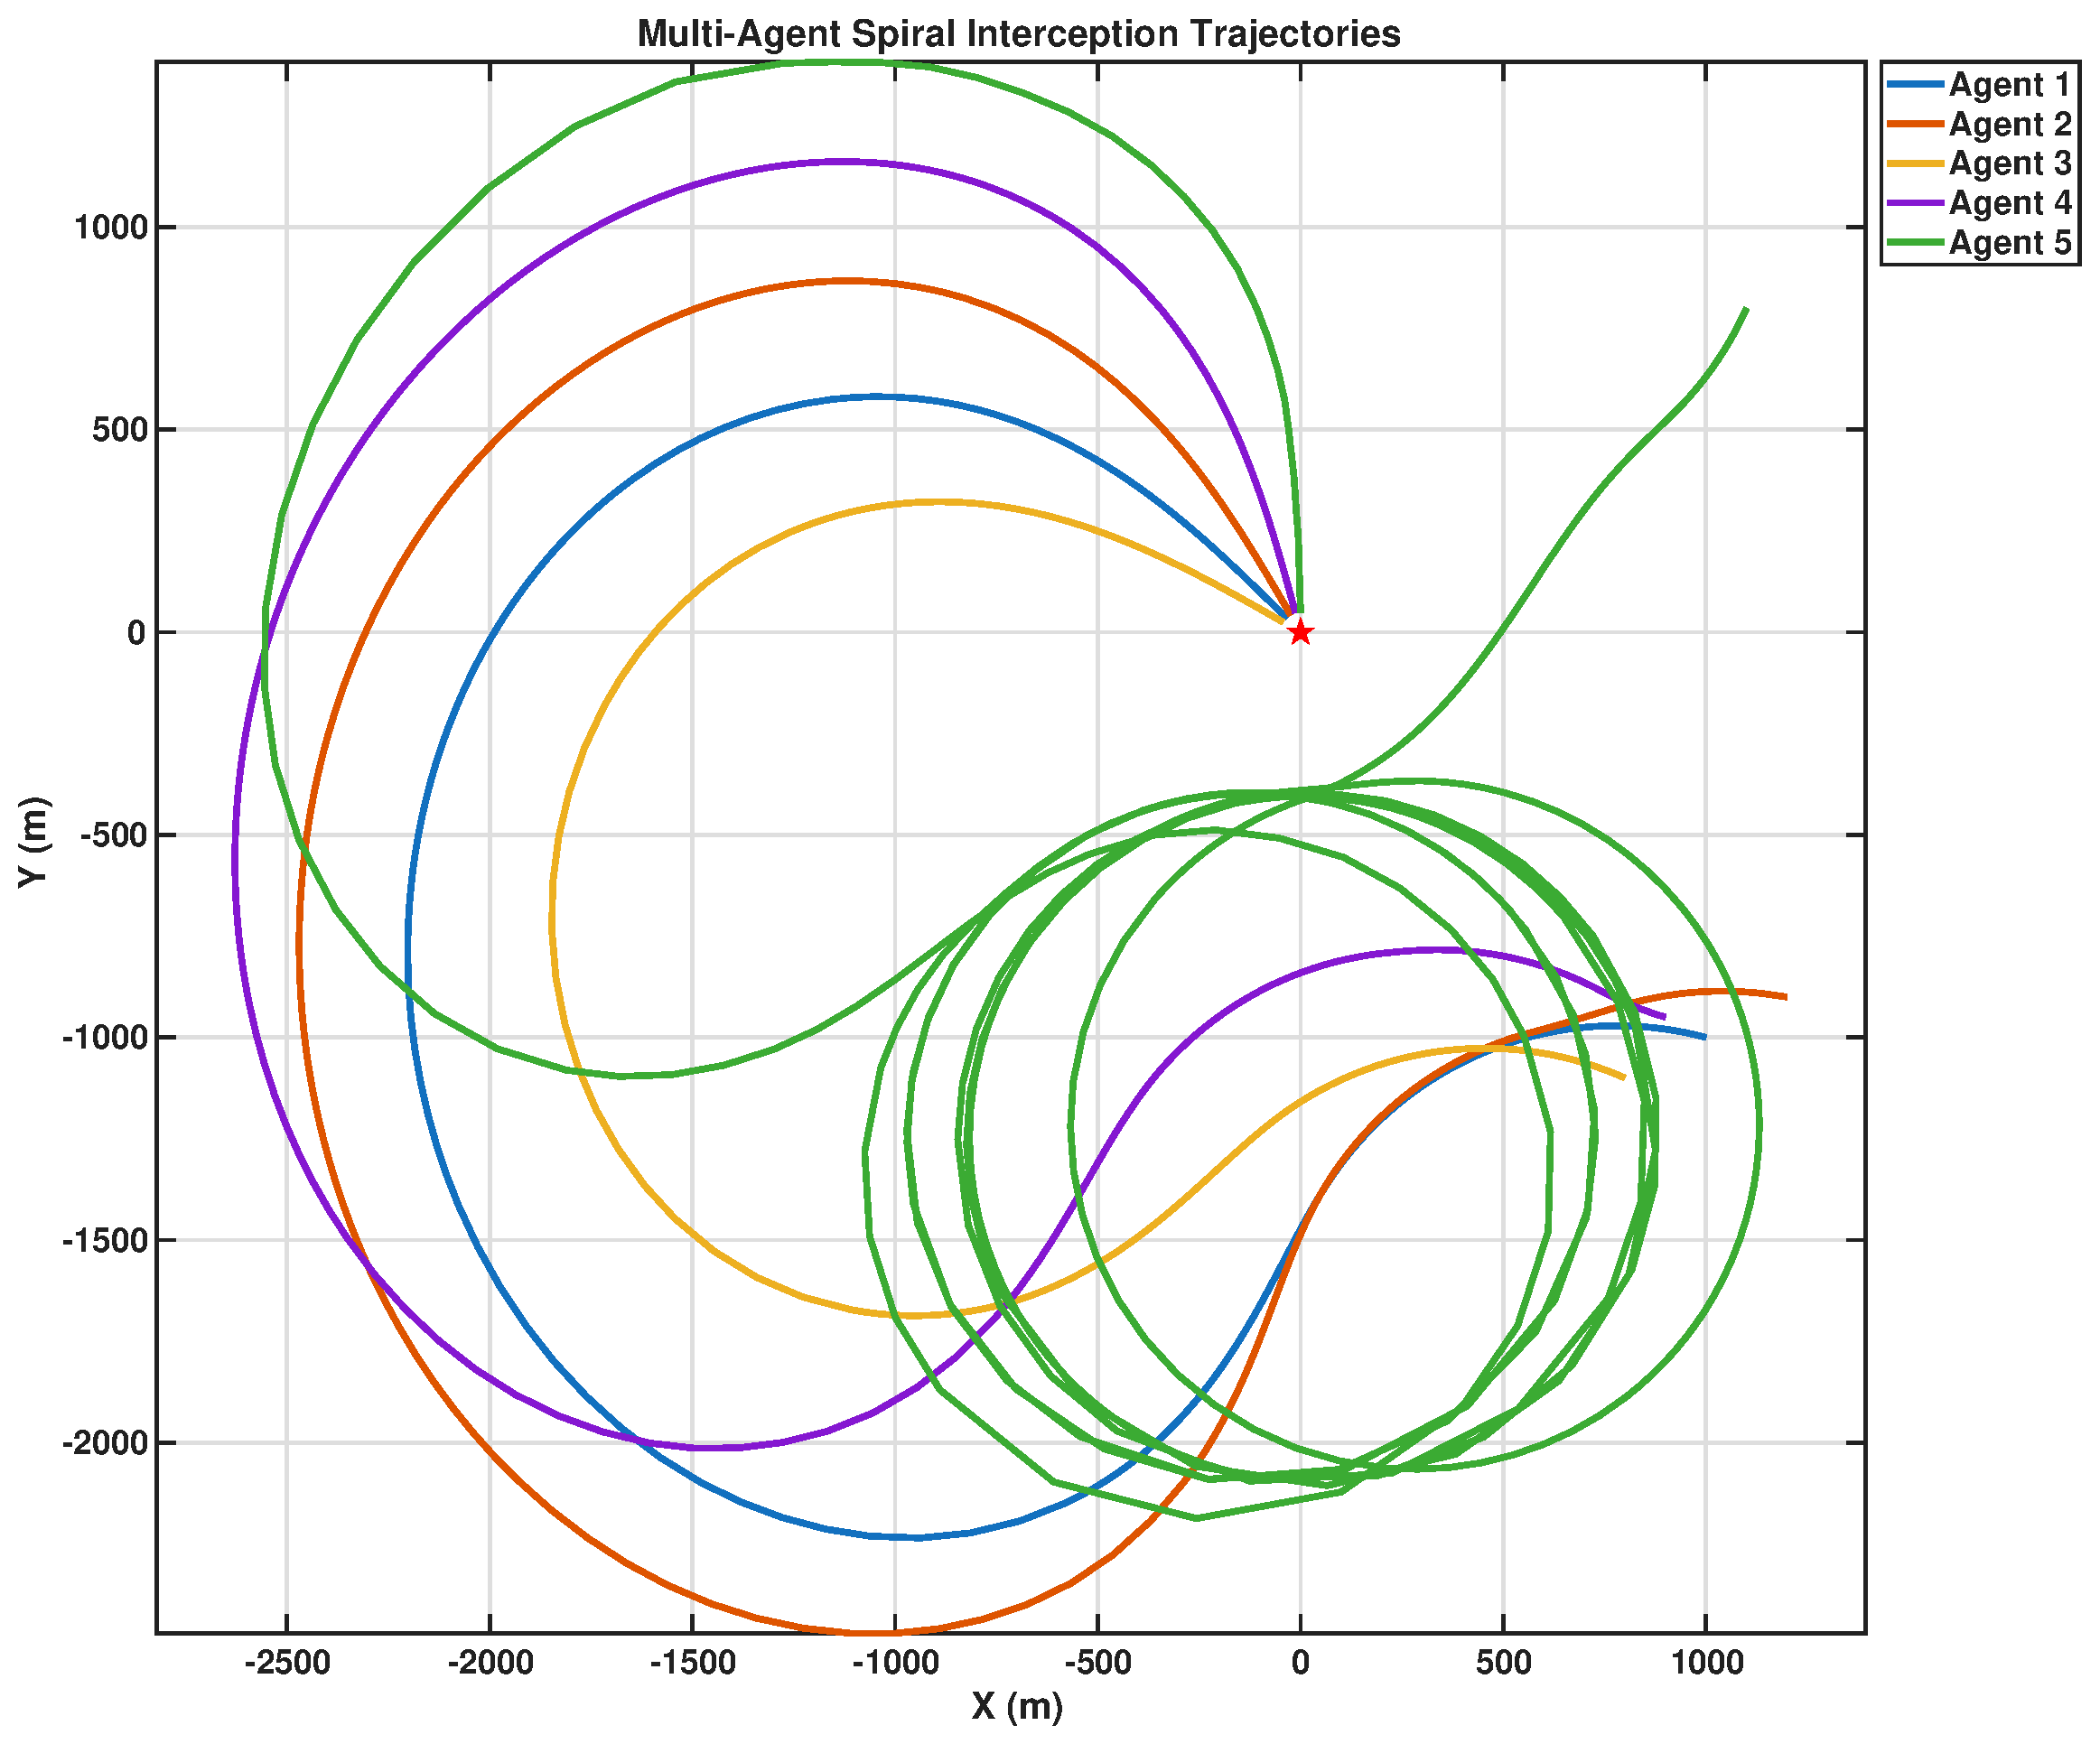
\includegraphics[scale=0.15]{Images/4Agent_Case7_Trajectory.eps}
				\caption{Trajectory of 5 Agents with Impact Angle in Same Sector}
			\end{figure}
		\end{column}
	\end{columns}
	
\end{frame}
%%%%%%%%%%%%%%%%%%%%%%%%%%%%%%%%%%%%%%%%%%%%%%%%%%%%%
%%%%%%%%%%%%%%%%%%%%%%%%%%%%%%%%%%%%%%%%%%%%%%%%%%%%%
\begin{frame}{}
	\begin{myblock}{Conclusion}
		\begin{itemize}
			\item We successfully developed a novel two-phase guidance law for high-precision impact angle control under strict actuator constraints.
			\item The key innovation is a proactive, "feasibility-seeking" first phase, which uses the vehicle's physical limits ($a_{max}$) to plan a guaranteed-flyable trajectory from the start.
			\item A robust, prescribed-time controller ensures the vehicle acquires and tracks the safe spiral path, successfully preventing control saturation and mission failure.
			\item A consensus based law proposed to extend it to multi-agent system.
			\item The consensus and topology ensures the scalability and directional interception.
			\item The chain topology also ensures that the interception occurs even if there is a link/node failure.
			%\item The proposed method was validated in simulation, demonstrating superior performance and robustness compared to simpler, single-phase guidance strategies.
		\end{itemize}
	\end{myblock}
	\begin{myblock}{Future Work}
		\begin{itemize}
		%	\item Develop the coordination algorithm for multi-agent system.
			\item Extend the framework to include simultaneous impact time control, creating a complete three-phase guidance solution.
		\end{itemize}
	\end{myblock}
	
\end{frame}
%%%%%%%%%%%%%%%%%%%%%%%%%%%%%%%%%%%%%%%%%%%%%%%%%%%%%
\begin{subframe}\label{Corr} %[noframenumbering] {Corrective Prescribed Time Control}
	\vspace{-0.3cm}
	\begin{figure}
		\centering
		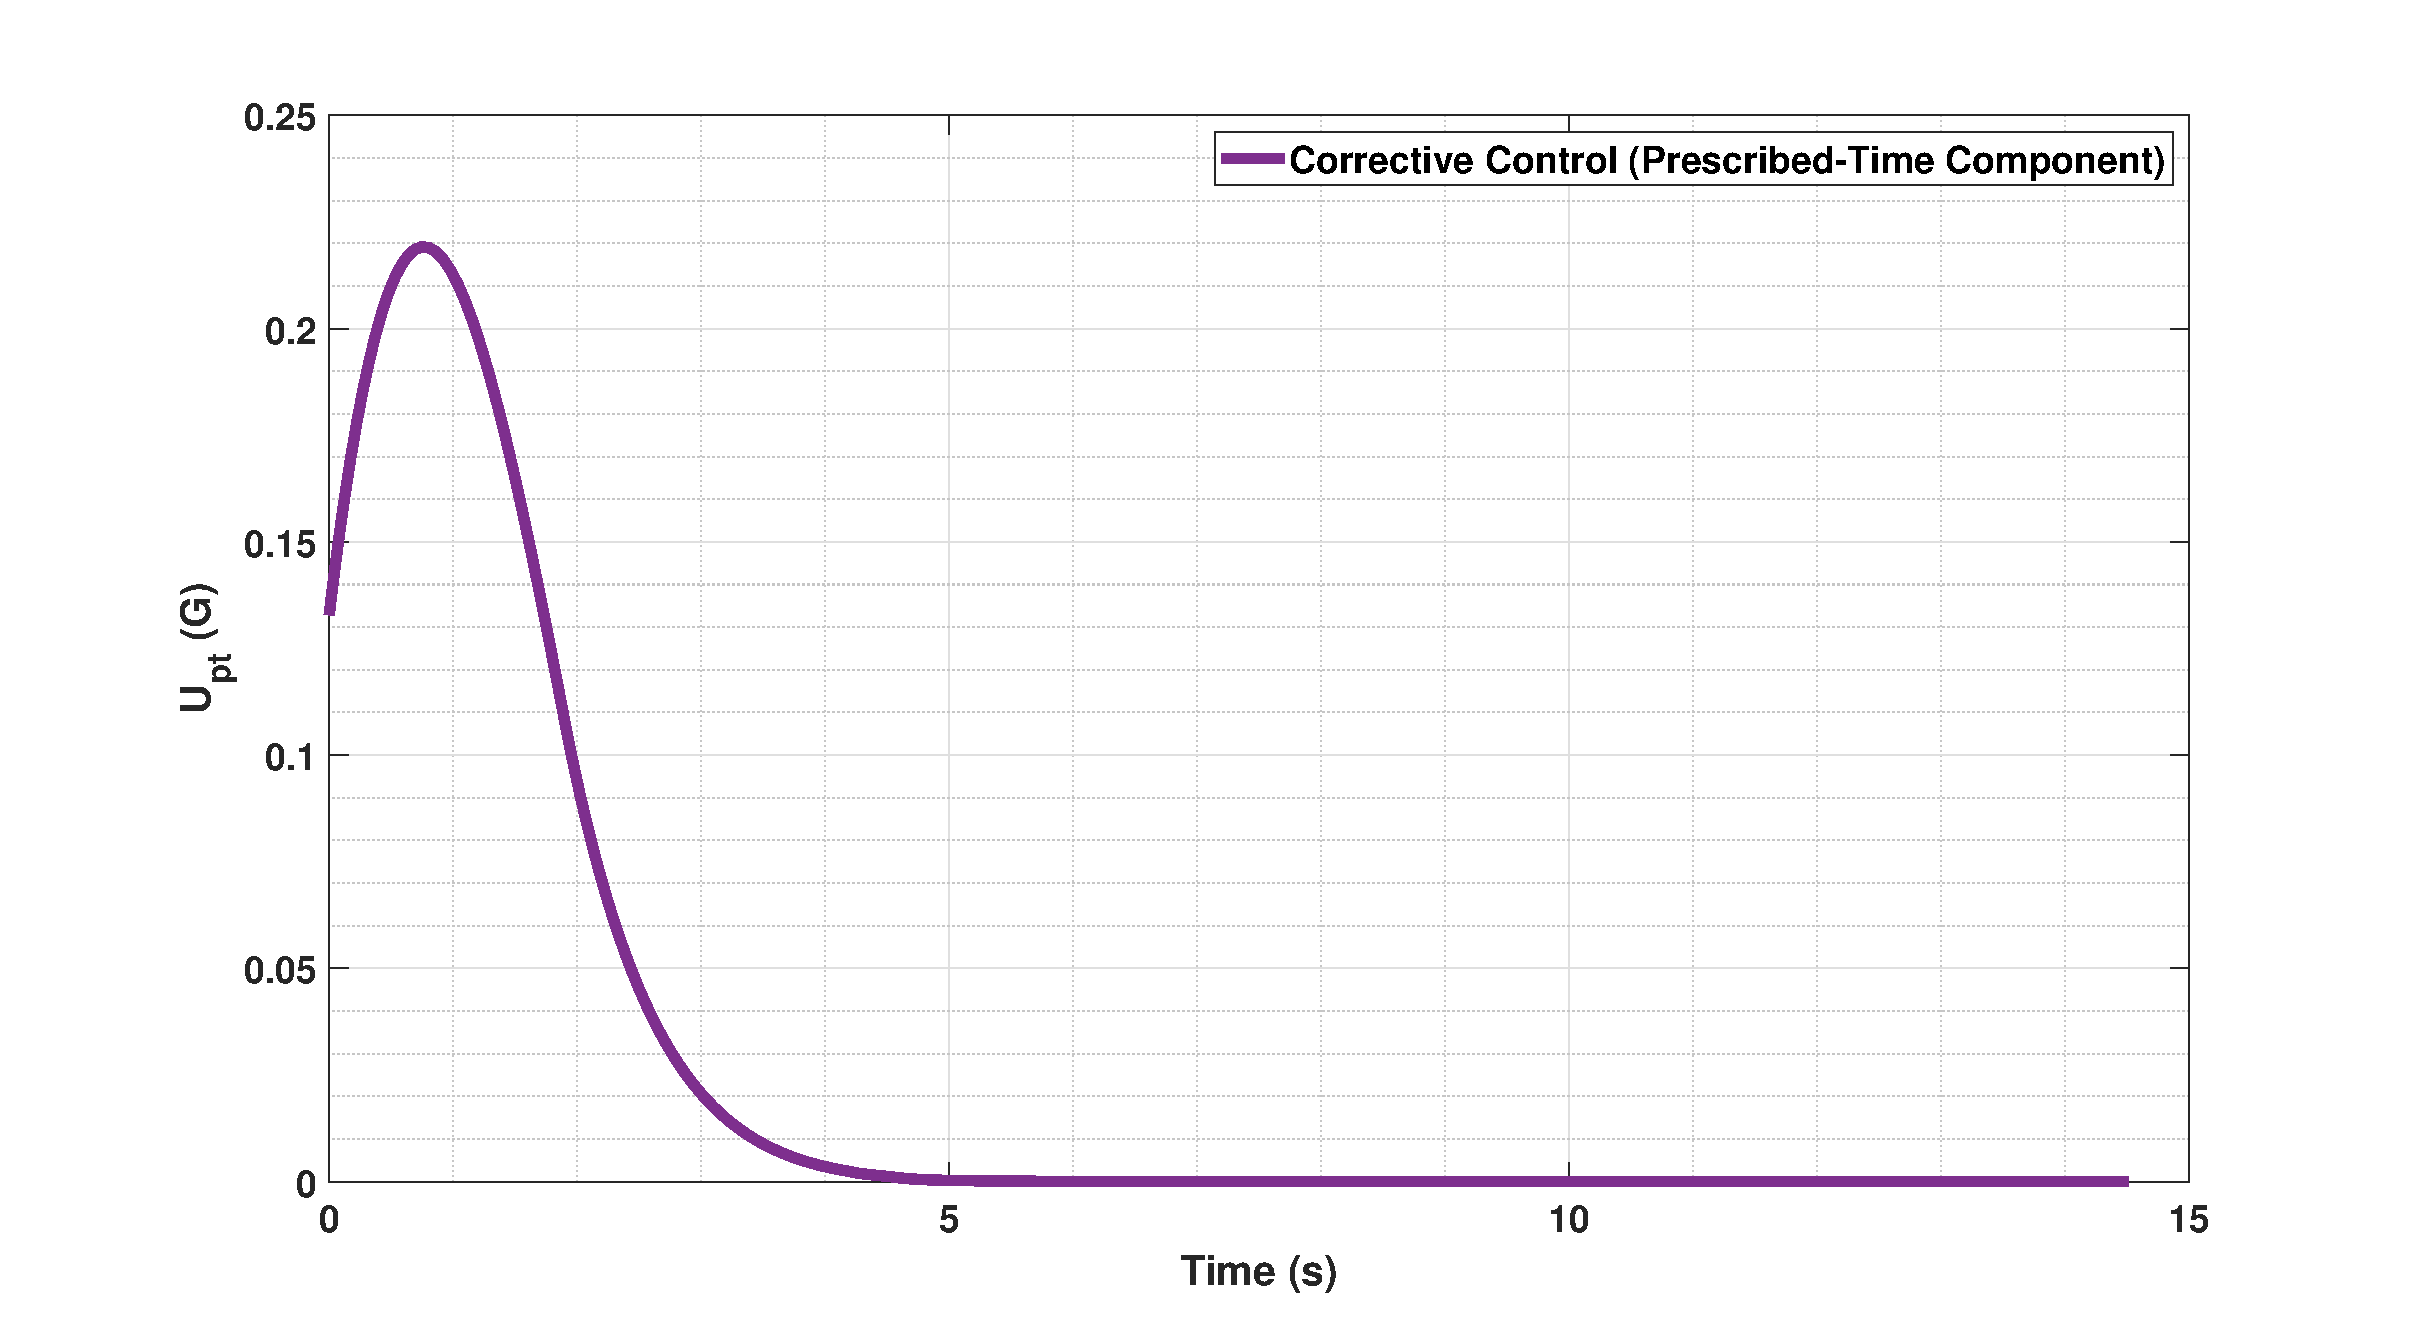
\includegraphics[scale=0.3]{Images/Correc_Control.eps}
	\end{figure}
	\hyperlink{Control}{\beamerbutton{Back}}
\end{subframe}
%----------------------------------------------------------------------------------------

% 
%\appendix
\subsection*{Containment Control in 3-D space}\label{Containment}
\begin{frame}{Containment of Double Integrators in 3D Space~~\hyperlink{Conc3DContainment}{\beamerbutton{Conclusion-3D}}~~\hyperlink{2DContainment}{\beamerbutton{PPT-2D}}}\label{3DContainment}
	%\vspace{-0.2cm}
	\begin{block}{}
		\begin{columns}
			\begin{column}{0.7\textwidth}
		~- Swarm of agents/drones are in 3D space.\\
		~- Trajectory to traverse known to selected few (\textcolor{blue}{Leaders})\\
		~- \textcolor{red}{Objective:} Plan trajectories for other agents such that they always remains inside the convex hull of the leaders.\\
		%\vspace{-0.2cm}
		\end{column}
		\begin{column}{0.3\textwidth}
		\begin{figure} 
			\centering
			\includegraphics[scale=0.2,keepaspectratio]{Swarm.png}
			%\caption{Swarm of drones following the trajectory defined by the leader drones}
			\label{Swarm}
		\end{figure}
		\end{column}
		\end{columns}
	\end{block}
	%\vspace{-0.2cm}
	\begin{block}{}
		- Leader Set:  $\mathcal{M}=\{1,2,\dots,M\}$,~~ Follower Set:  $\mathcal{N}=\{M+1,M+2,\dots, M+N\}$ \\
		- Position of Leaders and followers: $p_{i}(t), i \in \mathcal{M}\cup \mathcal{N}$ at time $t$\\
		- Convex hull of the leaders at any given time $t$ is defined by:
		\vspace{-0.3cm}
		$$co_{L}(t)=co\{p_{1}(t),\dots,p_{M}(t)\}=\sum_{i} \sigma_{i}p_{i}(t)|\sum_{i }\sigma_{i}=1, \sigma_{i}\geq 0, i \in \mathcal{M}$$
		\vspace{-0.3cm}
		- Containment Solution:$$\lim_{t\to\infty} \text{dis}(p_{i}(t),co_{L}(t))=0,i\in \mathcal{N}$$
	\end{block}
\end{frame}
\begin{frame}
	\vspace*{-0.3cm}
	\begin{block}{Assumptions}
		\begin{enumerate}
			\item Followers have the relative information only from their neighborhood.
			\item Either there exists a directed edge from any of the leaders to all but one follower, or some indirect path from one of the leaders to each follower. %In the second case, the topology among followers is \emph{strongly connected}.
			\item There exist a topological ordering.
		\end{enumerate}
	\end{block}
	\vspace*{-0.2cm}
	\begin{block}{Proposition 1\footnotemark[1]}
		The graph Laplacian with $M$ leaders and $N$ followers of the graph $\mathcal{G}$ is written as %~\footnotemark[1]
		$
			\mathcal{L}_{\mathcal{G}}=
			\begin{bmatrix}
				\boldsymbol{0} & \boldsymbol{0}\\
				\mathcal{L}_{1} & \mathcal{L}_{2}
			\end{bmatrix},
		$
		Under assumptions mentioned above:
		\begin{enumerate}
			\item All eigenvalues of $\mathcal{L}_{2}$ have positive real parts, thus validating the matrix to be invertible and hence $\mathcal{L}_{2}^{-1}$ exists.\textcolor{blue}{ (Important for invertibility of $\mathcal{L}_{2}$)}
			\item Each entry of $-\mathcal{L}_{2}^{-1}\mathcal{L}_{1} \geq 0$ and the row sum of every row equals to $1$. \textcolor{blue}{(Elements of row corresponds to $\sigma_{i}$)}
		\end{enumerate}
		where $\mathcal{L}_{1} \in \mathbb{R}^{N \times M}$, $\mathcal{L}_{2} \in \mathbb{R}^{N \times N}$, while $\boldsymbol{0}$ is a matrix of all zero entries, of appropriate dimension.
	\end{block}
	\footnotetext[1]{\textcolor{blue}{Meng, Z., Ren, W., \& You, Z.}, {\em Distributed finite-time attitude containment control for multiple rigid bodies}, Automatica, 46(12) 2010.}
	%\alt<2>{\let\thefootnote\relax\footnotetext{~}}{\footnotetext[1]{\textcolor{blue}{Meng, Z., Ren, W., \& You, Z.}, {\em Distributed finite-time attitude containment control for multiple rigid bodies}, Automatica, 46(12) 2010.}}
\end{frame}

\begin{frame}{}
		\vspace{-0.5cm}
	\begin{columns}
		\begin{column}{0.45\textwidth}
			\begin{block}{Leader's Dynamics}
				- Leaders dynamics are controllable and observable\\
				- Trajectory of $i^{th}$ leader is given by:
				$$	p_{i}(t)=c_{0}^{i}+c_{1}^{i}t+\dots+c_{n}^{i}t^{n},$$
				$\text{ where} \: i \in \mathcal{M},\: c_{j}^{i}\in \mathbb{R}^{3},\: j= 0,1,\dots,n$\\
				- $(n+1)$ points required to generate trajectory.\\
				- Leaders are considered as reference signals.
			\end{block}
		\end{column}
		\begin{column}{0.45\textwidth}
			\begin{block}{Followers' Dynamics}
				Motion dynamics of $i^{th}$ agent or the $(i-M)^{th}$ follower is given by:\\
				\begin{center}
					%\begin{equation}\label{Homodynamics}
					$\dot{Z_i}(t)=A_iZ_{i}(t)+Bu_{i}(t)+\delta_{i}(t)$,\\
					$y_i(t)=CZ_i(t)$
				\end{center}
				%\end{equation}
				%\begin{equation}
				%	y_i(t)=C_iZ_i(t)
				%\end{equation}
				Position and velocity of $(i-M)^{th}$ follower:
				$$p_{i}(t)=[Z_{i}(1)(t)]^T,~ v_{i}(t)=[Z_{i}(2)(t)]^T\in \mathbb{R}^{3}$$
			\end{block}
		\end{column}
	\end{columns}
	\vspace*{0.2cm}
	where $A_i=
	\begin{bsmallmatrix}
		0 & 1\\
		\alpha_{i} & \beta_{i}
	\end{bsmallmatrix}$
	and $B=
	\begin{bsmallmatrix}
		0 \\ 1
	\end{bsmallmatrix}$,
	$C=
	\begin{bsmallmatrix}
		1 & 0
	\end{bsmallmatrix}$,
	$Z_{i} \in \mathbb{R}^{2}$, $u_i \in \mathbb{R}$. \\
	$\delta_{i}(t)=d_{0}^{i}+d_{1}^{i}t+\dots+d_{r}^{i}t^{r},\: r\in \mathbb{N}, \: d_{j}^{i}\in \mathbb{R}^{2},\: j=0,1,\dots,r$ is the polynomial type disturbance.
	\end{frame}
	\begin{comment}
	\begin{block}{Leader's Dynamics}
		- Leaders dynamics are controllable and observable\\
		- Trajectory of $i^{th}$ leader is given by:
		$$	p_{i}(t)=c_{0}^{i}+c_{1}^{i}t+\dots+c_{n}^{i}t^{n},\text{ where} \: i \in \mathcal{M},\: c_{j}^{i}\in \mathbb{R}^{3},\: j= 0,1,\dots,n$$
		- $(n+1)$ points required to generate trajectory.\\
		- Leaders are considered as reference signals.
	\end{block}
	%\vspace{-0.1cm}
	\begin{block}{Followers' Dynamics}
		Motion dynamics of $i^{th}$ agent or the $(i-M)^{th}$ follower (second-order linear dynamics) is given by:\\
		\begin{center}
			%\begin{equation}\label{Homodynamics}
			$\dot{Z_i}(t)=A_iZ_{i}(t)+Bu_{i}(t)+\delta_{i}(t)$,\\
			$y_i(t)=CZ_i(t)$
		\end{center}
		%\end{equation}
		%\begin{equation}
		%	y_i(t)=C_iZ_i(t)
		%\end{equation}
		where $A_i=
		\begin{bsmallmatrix}
			0 & 1\\
			\alpha_{i} & \beta_{i}
		\end{bsmallmatrix}$
		and $B=
		\begin{bsmallmatrix}
			0 \\ 1
		\end{bsmallmatrix}$,
		$C=
		\begin{bsmallmatrix}
			1 & 0
		\end{bsmallmatrix}$,
		$Z_{i} \in \mathbb{R}^{2}$, $u_i \in \mathbb{R}$. \\
		$\delta_{i}(t)=d_{0}^{i}+d_{1}^{i}t+\dots+d_{r}^{i}t^{r},\: r\in \mathbb{N}, \: d_{j}^{i}\in \mathbb{R}^{2},\: j=0,1,\dots,r$ is the polynomial type disturbance.\\
		The position and velocity of $(i-M)^{th}$ follower is given by
		$$p_{i}(t)=[Z_{i}(1)(t)]^T,v_{i}(t)=[Z_{i}(2)(t)]^T\in \mathbb{R}^{3}$$
	\end{block}	
\end{comment}

\begin{frame}{}
	%\vspace{-0.1cm}
	\begin{block}{Proposed Control Law}
		$$  u_{i}(t)=\sum_{l=0}^{l_{m}-1}k_{l}\mathcal{D}^{1-l}\sum_{j \in \mathcal{M}\cup \mathcal{N}}\alpha_{ij} e_{ji}(t)$$
		%\end{equation}
		where $e_{ji}=p_j(t)-p_i(t)$ and $\mathcal{D}$ denotes the derivative operator.\\
		- The above equation has \textcolor{blue}{one derivative term, one proportional term, and $l_{m}-2$ integral terms}.\\ 
		- Since the order of the follower is assumed to be 2, therefore, $l_{m}=\max(2,n+1)$, where $n$ is the order of leader's trajectory.
	\end{block}
	%\vspace{-0.1cm}
	%\textbf{Note: }{
		\begin{block}{Agent's Dynamics Individually}
			Let $\xi_{i}(t)=(p_{i}^{T}(t),p_{i}^{(1)T}(t),\dots, p_{i}^{(l_{m}-1)T}(t))^T$. Then dynamics of $i^{th}$ agent can be described by:\\
			$~~~\color{cyan}{\dot{\xi_{i}}(t)=(E\otimes I_{3})\xi_{i}(t), \: \: i \in \mathcal{M}},~~~\color{brown}{\dot{\xi_{i}}(t)=(E \otimes I_{3})\xi_{i}(t)+(B \otimes I_{3}) \bar{u_{i}}(t)+\mathcal{D}^{l_{m}-2}\delta_{i}(t), \: \:  i \in \mathcal{N}}$\\
			\vspace*{0.2cm}
			where $E=\begin{bsmallmatrix}
				0 & 1 & 0 & \dots & 0\\
				0 & 0 & 1 & \dots & 0\\
				\vdots & \vdots & \vdots & \vdots & \vdots\\
				0 & 0 & 0 & \dots & 1 \\
				0 & 0 & 0 & \dots & 0
			\end{bsmallmatrix} \in \R^{(n+1) \times (n+1)},~~~
			B=\begin{bsmallmatrix}0 \\ 0 \\ \vdots \\ 0 \\ 1 \end{bsmallmatrix} \in \R^{n+1},$\\
			\vspace*{0.2cm}
			$~~~\bar{u}_{i}=\mathcal{D}^{(l_m-2)}u_{i}(t)=\sum_{j}K(\xi_{j}(t)-\xi_{i}(t)), ~~~\: j \in \mathcal{M}\cup \mathcal{N}, ~~~\: K=\begin{bsmallmatrix}k_n & \dots & k_1 & k_0 \end{bsmallmatrix}$
		\end{block}
		
	\end{frame}
	\begin{frame}{Stacked Dynamics}%\label{BL}
		\vspace{-0.2cm}
		\begin{block}{}
			Let $\Xi_L(t)= (\xi_1^T(t),\xi_2^T(t),\dots, \xi_M^T(t))^T$, then the Stacked Leaders' Dynamics are:
			$$\boxed{\mathcal{D}\Xi_{L}(t)= (I_{M} \otimes E \otimes I_{3})\Xi_{L}(t)}$$
			Let $\Xi_F(t)= (\xi_{M+1}^T(t), \xi_{M+2}^T(t), \dots, \xi_{M+N}^T(t))^T$ then the Stacked Followers' Dynamics are:
			$$\boxed{\mathcal{D}\Xi_{F}(t)= (\mathcal{I}_{\mathcal{N}} \otimes E \otimes I_{p}-\mathcal{L}_2 \otimes BK \otimes I_{p}) \Xi_{F}(t) - (\mathcal{L}_1 \otimes BK \otimes I_{p}) \Xi_{L}(t)+ (I_{N} \otimes B \otimes I_{p}) \Delta(t)}$$
			Taking $\hat{\Xi}_{F}(t)=\Xi_{F}(t)+(\mathcal{L}_2^{-1}\mathcal{L}_1 \otimes I_{(n+1)p})\Xi_{L}(t)$, we get 
			%			\begin{equation}
				$$\boxed{\mathcal{D}\hat{\Xi}_{F}(t)=(\mathcal{I}_{\mathcal{N}} \otimes E \otimes I_{p}-\mathcal{L}_2 \otimes BK \otimes I_{p})\hat{\Xi}_{F}(t)+(I_{N} \otimes B \otimes I_{p})\Delta(t)}$$
				%			\end{equation}
			where $\Delta(t)$ is the diagonal matrix with $(l_{m}-2)^{th}$ derivative of noise terms $\delta(t)$ in the diagonal.\\
			$$\bar{u}_{i}=\mathcal{D}^{(l_m-2)} u_{i}(t)=\sum_{j}K(\xi_{j}(t)-\xi_{i}(t)), \:		j \in \mathcal{M}\cup \mathcal{N}, \: K=\begin{bsmallmatrix}k_n & \dots & k_1 & k_0 \end{bsmallmatrix}$$
		\end{block}
		\pause
		%$H=(\mathcal{I}_{\mathcal{N}} \otimes E \otimes I_{p}-\mathcal{L}_2 \otimes BK \otimes I_{p})$,
		%$P=(\mathcal{L}_1 \otimes BK \otimes I_{p})$,
		%$L=(I_{N} \otimes B \otimes I_{p})$,\\
		%$W=\mathcal{I}_{\mathcal{N}} \otimes E-\mathcal{L}_2\otimes BK$.
		%\begin{alertblock}{Containment Solution}
		%Solving for the containment problem is equivalent to ensuring that matrix $$\mathcal{I}_{\mathcal{N}} \otimes E \otimes I_{p}-\mathcal{L}_2 \otimes BK \otimes I_{p}$$ being hurwitz.
		%\end{alertblock}
		\textcolor{blue}{Containment Solution: }\\
		- Ensure the matrix $(\mathcal{I}_{\mathcal{N}} \otimes E -\mathcal{L}_2 \otimes BK) \otimes I_{p} \implies $ \textcolor{red}{$ \mathcal{I}_{\mathcal{N}} \otimes E-\mathcal{L}_2 \otimes BK$ is Hurwitz.\\
			- $\Delta(t)$ doesn't affect the dynamics}: achieved if noise is a polynomial of degree $(l_{m}-3)$\\
		%If we assume that the noise is a polynomial of degree $(l_{m}-3)$, its effect can be nullified, because $(l_{m}-3)^{\text rd}$ derivative becomes 0.
	\end{frame}
	%\againframe<2>{base}
	\begin{frame}{Recall}
		\vspace{-0.2cm}
		\begin{block}{}
			- Graph Laplacian 
			$\mathcal{L}_{\mathcal{G}}=
			\begin{bmatrix}
				\boldsymbol{0} & \boldsymbol{0}\\
				\mathcal{L}_{1} & \mathcal{L}_{2}
			\end{bmatrix}$\\
			- Under topological ordering constraints $\mathcal{L}_2$ is lower triangular $ \implies (\mathcal{I}_{\mathcal{N}} \otimes E-\mathcal{L}_2 \otimes BK$) is also lower triangular block matrix.
		\end{block}
		\vspace*{-0.2cm}
		%\alt<2>{\let\thefootnote\relax\footnotetext{~}}{\footnotetext[1]{\textcolor{blue}{Meng, Z., Ren, W., \& You, Z.}, {\em Distributed finite-time attitude containment control for multiple rigid bodies}, Automatica, 46(12) 2010.}}
		\begin{exampleblock}{}
			- Follower Dynamics is $$\dot{Z_i}(t)=A_iZ_{i}(t)+B_iu_{i}(t)+\delta_{i}(t)$$
			where $A_i=
			\begin{bsmallmatrix}
				0 & 1\\
				\alpha_{i} & \beta_{i}
			\end{bsmallmatrix}, ~~~\:B=
			\begin{bsmallmatrix}
				0 \\ 1
			\end{bsmallmatrix}$,\\
			- \textcolor{blue}{Objective: }Stabilizing $N$ different polynomials of order $l_{m}$.\\
			- Characteristic equation of $(i-M)^{\rm th}$ block of the matrix ($\mathcal{I}_{\mathcal{N}} \otimes E-\mathcal{L}_2 \otimes BK$) is given by:
			$$\color{cyan}{s^{l_{m}}+(k_{0}\lambda_{i}-\beta_{i})s^{l_{m}-1} +(k_{1}\lambda_{i}-\alpha_{i})s^{l_{m}-2}}+\color{brown}{(k_{2}\lambda_{i})s^{l_{m}-3}+\dots+(k_{l_{m}-1}\lambda_{i})}=0,$$
			$
				\implies 1+ \frac{\color{brown}{k_{2}\lambda_{i}(s^{l_{m}-3}+\hat{k}_{3}s^{l_{m}-4}+\dots+\hat{k}_{l_{m}-1})}}{\color{cyan}{s^{l_{m}-2}(s^2 + (k_{0}\lambda_{i}-\beta_{i})s)+(k_{1}\lambda_{i}-\alpha_{i})}}=0,~~~
			$ where, $\lambda_{i}$ is the $i^{th}$ eigenvalue of matrix $\mathcal{L}_2$\\
		%	- Since $(2)$ is of $1+G(s)=0$ form, we can use root locus to solve the problem.
		\end{exampleblock}
	\end{frame}
	
	%%%%%%%%%%%%%%%%%%%%%%%%%%%%%%%%%%%%%%%%%%%%%%%%%%%%%%%%%%%%%%%%%%%%%%%%%%%%%%%%%%%%%
	\begin{frame}{Algorithm}
		$$1+G(s)= 1+ \frac{k_{2}\lambda_{i}(s^{l_{m}-3}+\hat{k}_{3}s^{l_{m}-4}+\dots+\hat{k}_{l_{m}-1})}{s^{l_{m}-2}(s^2 + (\lambda_{i}k_{0}-\beta_{i})s)+(\lambda_{i}k_{1}-\alpha_{i})}=0.$$
		Challenge is to design single controller gain $K$, which stabilizes all the $M$ blocks.
		\begin{block}{}
			\begin{itemize}
				\item First fix values of $k_{0}$ and $k_{1}$ such that the two closed loop poles which are not at origin are at left hand side of imaginary axis for all the N agents.
				\item Fix elements of $[1, \hat{k}_{3},\dots, \hat{k}_{l_{m}-1}]$ such that all the $l_{m}-3$ zeros are on the right side of the original poles of the systems and left side of origin, such that the two branches of root loci going to right side of the imaginary plane have a portion inside the left side of imaginary axis. This is the range of gains for which system is stable.
				\item Select a common gain that stabilizes all the $M$ blocks, and assign this value to $k_{2}$.
				\item Now, we can calculate all other remaining gains in the matrix  $K$ from the numerator polynomial.
			\end{itemize} 
		\end{block}
		%\begin{block}{Conclusion}
		%	\begin{itemize}
			%		\item Designed single controller for all the followers.
			%		\item The proposed controllers not only works for heterogeneous followers but also when some of them have unstable dynamics.
			%		\item The proposed controller also nullifies the effect of noise.
			%	\end{itemize}
		%\end{block}
	\end{frame}
	%%%%%%%%%%%%%%%%%%%%%%%%%%%%%%%%%%%%%%%%%%%%%%%%%%%%%%%%%%%%%%%%%%%%%%%%%%%%%%%%%%%%
	\begin{frame}{Experimental Setup: Homogeneous Stable System}
		The leaders are assumed to follow a $5^{th}$ order polynomial trajectory, i.e., $n=5$ and $l_m=6$. Thus, the system can cancel out the effect of disturbances of order 3.
		\begin{figure}
			\centering
			\begin{minipage}{0.4\linewidth}
				\centering
				\includegraphics[width=\textwidth]{homo_stable_topology.jpg}
				\textnormal{(a). Topology for Homogeneous stable system}
			\end{minipage}
			\hspace{1em}
			\begin{minipage}{0.5\linewidth}
				%\centering
				- Consider a multi-agent system of 8 agents where agents 1 to 4 are leaders and agents 5 through 8, as shown in Figure, are the followers. \\
				- All the agents are assumed to be connected over an unweighted topology. \\
				- The system is considered as homogeneous and individual agents are stable with system matrix given by
				$$A=\begin{bmatrix}
						0 & 1 \\
						-10 & -20
				\end{bmatrix}.
				$$
			\end{minipage}\\
		\end{figure}
	\end{frame}
	%%%%%%%%%%%%%%%%%%%%%%%%%%%%%%%%%%%%%%%%%%%%%%%%%%%%%%%%%%%%%%%%%%%%%%%%%%%%%%%%%%%%%%%
	\begin{frame}{Simulation Results: Homogeneous Stable System Root Locus}
		\begin{figure}
			\centering
			%\begin{minipage}{0.6\linewidth}
			%\centering
			\includegraphics[scale=.25]{rlocus_stab_hom_1-4_final.eps}
			\caption{Followers in Homogeneous stable system}
			%\textnormal{(a). Rootlocus for }
			%\end{minipage}
			%\hspace{1em}
			%\begin{minipage}{0.4\linewidth}
			%\centering
			%\textnormal{(b). Containment Path of followers in Homogeneous stable system}
			%\end{minipage}
		\end{figure}
		The gain matrix $K=[0.63, 10.2, 55.31, 100, 100, 50]$
	\end{frame}
	\begin{frame}{Simulation Results: Homogeneous Stable System Path}
		\begin{figure}
			\includegraphics[scale=0.25]{path_stab_homo_final.eps}
			\caption{Path of followers in Homogeneous stable system}
		\end{figure}
		The gain matrix $K=[0.63, 10.2, 55.31, 100, 100, 50]$
	\end{frame}
	
	%%%%%%%%%%%%%%%%%%%%%%%%%%%%%%%%%%%%%%%%%%%%%%%%%%%%%%%%%%%%%%%%%%%%%%%%%%%%%%%%%%%%%%%
	\begin{frame}{Experimental Setup: Homogeneous Unstable System}
		\begin{figure}
			\centering
			\begin{minipage}{0.4\linewidth}
				\centering
				\includegraphics[width=0.8\textwidth]{unstable_topology.jpg}
				\textnormal{(a). Topology for Homogeneous unstable system}
			\end{minipage}
			\hspace{1em}
			\begin{minipage}{0.5\linewidth}
				%\centering
				- From the chosen topology, all the $\lambda's$ are identical and $\lambda=6$.\\ 
				- $ A=\begin{bmatrix} 0 & 1 \\ 100 & 400 \end{bmatrix}.$\\
				- Having identical $\lambda's$, need to stabilize only one root locus
			\end{minipage}\\
		\end{figure}
	\end{frame}
	%%%%%%%%%%%%%%%%%%%%%%%%%%%%%%%%%%%%%%%%%%%%%%%%%%%%%%%%%%%%%%%%%%%%%%%%%%%%%%%%%%%%%%%
	\begin{frame}{Simulation Results: Homogeneous Unstable System}
		\begin{figure}
			\centering
			\includegraphics[width=0.6\textwidth]{rlocus_unsta_homo_final.eps}
			\caption{(a). Rootlocus for Homogeneous unstable system}
			%\includegraphics[width=\textwidth]{path_unst_homo_final.eps}
			%	\caption{(b). Containment Path in Homogeneous unstable system}
		\end{figure}
		The gain matrix for solving the containment problem is $$K=[10^8, 3 \times 10^7, 3\times 10^6, 10^5, 1683.3, 100]$$
	\end{frame}
	\begin{frame}{Simulation Results: Homogeneous Unstable System}
		\begin{figure}
			\centering
			%\includegraphics[width=\textwidth]{rlocus_unsta_homo_final.eps}
			%\caption{(a). Rootlocus for Homogeneous unstable system}
			\includegraphics[width=0.6\textwidth]{path_unst_homo_final.eps}
			\caption{(b). Containment Path in Homogeneous unstable system}
		\end{figure}
		The gain matrix for solving the containment problem is $$K=[10^8, 3 \times 10^7, 3\times 10^6, 10^5, 1683.3, 100]$$
	\end{frame}
	%%%%%%%%%%%%%%%%%%%%%%%%%%%%%%%%%%%%%%%%%%%%%%%%%%%%%%%%%%%%%%%%%%%%%%%%%%%%%%%%%%%%%%%
	\begin{frame}{Experimental Setup: Heterogeneous Stable System}
		\begin{figure}
			\centering
			\begin{minipage}{0.4\linewidth}
				\centering
				\includegraphics[width=0.8\textwidth]{hetero_topology.jpg}
				\textnormal{(a). Topology for Heterogeneous system}
			\end{minipage}
			\hspace{1em}
			\begin{minipage}{0.5\linewidth}
				%\centering
				System matrices of the unstable followers are given as:\\
				$A_5=\begin{bmatrix}0 & 1 \\-4 & 5\end{bmatrix},~~~~~~ 
				A_6=\begin{bmatrix}0 & 1 \\-10 & 10\end{bmatrix}$, \\
				$A_7=\begin{bmatrix}0 & 1 \\20 & -20\end{bmatrix},~~~ 
				A_8=\begin{bmatrix}0 & 1 \\-2 & 7\end{bmatrix}$.\\
				
				
				The $\mathcal{L}_2$ matrix have $4$ (followers) different eigenvalues. So, we have to stabilize four root loci simultaneously. 
			\end{minipage}\\
		\end{figure}
	\end{frame}
	%%%%%%%%%%%%%%%%%%%%%%%%%%%%%%%%%%%%%%%%%%%%%%%%%%%%%%%%%%%%%%%%%%%%%%%%%%%%%%%%%%%%%%%
	\begin{frame}{Simulation Results: Heterogeneous Stable System}
		\begin{figure}
			\centering
			\includegraphics[width=0.6\textwidth]{rlocus_hetero1-4_final.eps}
			\caption{(a). Root locus for followers in Heterogeneous system}
			%\includegraphics[width=\textwidth]{path_hetero_final.eps}
			%\textnormal{(b). Containment Path of followers in Heterogeneous system}
		\end{figure}
		The gain matrix for solving the containment problem is $$K=[0.5975,36.5,739,5000,1000,2000]$$
	\end{frame}
	\begin{frame}{Simulation Results: Heterogeneous Stable System}
		\begin{figure}
			\centering
			%\includegraphics[width=\textwidth]{rlocus_hetero1-4_final.eps}
			%\textnormal{(a). Root locus for followers in Heterogeneous system}
			\includegraphics[width=0.6\textwidth]{path_hetero_final.eps}
			\caption{(b). Containment Path of followers in Heterogeneous system}
		\end{figure}
		The gain matrix for solving the containment problem is $$K=[0.5975,36.5,739,5000,1000,2000]$$
	\end{frame}
	\begin{frame}{Conclusion \& Future Work}\label{Conc3DContainment}
		\begin{block}{Conclusion}
			\begin{itemize}
				\item Designed single controller for all the followers.
				\item The proposed controllers not only works for heterogeneous followers but also when some of them have unstable dynamics.
				\item The proposed controller also nullifies the effect of noise.
			\end{itemize}
		\end{block}
		\vspace*{-0.2cm}
		\begin{block}{Future Work}
			\begin{itemize}
				\item Apply systematic approach to include non-identical heterogeneous follower to truly address the problem of heterogeneity.\vspace{2mm}
				\item Implement the collision avoidance technique to prevent any accident among the followers.\vspace{2mm}
				\item Using the directed topology including the directed cycles.\vspace{2mm}
				\item Extend the result to weakly connected follower topology.\vspace{2mm}
			\end{itemize}
		\end{block}
		\hyperlink{3DContainment}{\beamerbutton{BackTo3DContainment}}
	\end{frame}
%%%%%%%%%%%%%%%%%%%%%%%%%%%%%%%%%%%%%%%%%%%%%%%%%%%%%%%%%%%%%%%%%%%%%%%%%%%%%%%%%%%%%%%%%%%%%%%%%%%%%%%%%%%%

	\subsection*{Containment of Double Integrators in 2D Space}\label{2DContainment}
	\begin{frame}{Containment Control for Terrestrial Robots:2D Case}
		\begin{block}{}
			- Swarm of agents/robots in 2D space.\\
			- Trajectory to traverse known to selected few (\textcolor{blue}{Leaders})\\
			- \textcolor{red}{Objective:} Plan topology and trajectories for followers such that they always remains inside the convex hull of the leaders.\\
		\end{block}
		%\begin{center}
		%	\includegraphics[scale=0.3,keepaspectratio]{TSwarm.png}
		%\end{center}
		\begin{block}{Proposed Method}
			\begin{enumerate}
				\item Designing a suitable network topology for containment.
				\item Using a polynomial based approach for agents to follow the convex hull.
			\end{enumerate}
		\end{block}
		
	\end{frame}
	\begin{frame}{Background}
		\vspace{-0.2cm}
		\begin{block}{Proposition 1~\footnotemark[1]}
			Let $P(x)$ be a polynomial with complex coefficient. Then the roots of derivative polynomial $P'(x)$ belongs to the convex hull of the roots of the polynomial P itself.
		\end{block}
		\vspace{-0.2cm}
		\begin{block}{Proposition 2~\footnotemark[1]}
			If $P(x)$ has distinct root, then the roots of derivative polynomial $P'(x)$ are distinct than the roots of P(x).
		\end{block}
		\vspace{-0.2cm}
		\begin{block}{Lemma 3}
			With two distinct point inside a triangle T, five distinct non-overlapping triangle can be created inside T.\\
			\centering
			\includegraphics[scale=0.3,keepaspectratio]{nonoverlaptriangle.eps}  	
		\end{block}
		\footnotetext[1]{Prasolov, V. V. (2004). Polynomials. Germany: Springer.}
	\end{frame}
	
	
	\begin{frame}{}
		\begin{block}{Assumptions}
			\begin{enumerate}
				\item The agents/robots measure only relative position from a subset of leaders.
				\item Each leader starts at a distinct position i.e. no two agents start at the same positions.
				\item Leaders hold the shape of the convex hull at all time.
				\item The network among the agents is directed.
				\item The agents are modeled as double integrators.
			\end{enumerate}
		\end{block}
		\begin{alertblock}{Strategy}
			Let there be $M$ leaders whose positions are given by $x_1,x_2,\dots,x_m$. Form a polynomial $$P(x)=\prod_{i=1}^{m}(x-x_i)$$
			Then the target position of $m-1$ followers will be given by roots of $P'(x)=0$, where $P'(x)$ is the derivative of $P(x)$ with respect to $x \in \C$.\\
		\end{alertblock}
	\end{frame}
	
	\begin{frame}{Apparent Problems}
		\begin{itemize}
			\item The idea seems to only accommodate $m-1$ followers i.e. less followers than the number of leaders. \\
			\textcolor{blue}{ Probable Solution:} 
			\begin{enumerate}
				\item Create a layered structure i.e. making the $m-1$ followers as leaders for next $m-2$ followers and repeating the procedure. However, using this method we can accommodate at max  $m(m-1)/2$ followers and $m-k$ followers at the $k^{th}$ layer.
				\item Other Solution is to create the layered structure by taking all the $m+m-1=2m-1$ agents as leaders for the next $2(m-1)$ followers. This way we can accommodate any number of followers. For calculations, $2^k(m-1)$ followers at the $k^{th}$ layer. 
			\end{enumerate}
			\item All followers needs to have connection with the leaders. If we try to increase the number using layered structure, then all the agents at $k^{th}$ layer should be connected to all the agents at $(k-1)^{th}$ layer. So the number of connections required will be $\frac{m^3-m}{3}=\mathcal{O}(3)$ for the first case and of $\mathcal{O}(4^k)$ at $k^{th}$ layer in second case. 
			\item There might be multiple followers approaching the same point and may collide among them.
		\end{itemize}
	\end{frame}
	
	\begin{frame}
		\begin{block}{Proposed Algorithm}
			\begin{enumerate}
				\item Divide the convex polygon formed by $m$ leaders into $m-2$ non-overlapping triangles. 
				\item Index all the followers and pair them up. If there are odd number of follower then pair the last one with a virtual follower. 
				\item Pick agents forming each set of triangle and compute the two position for the followers and place one pair of follower in each triangle.
				\item For conflict resolution, the rules can be laid down as given below:
				\begin{itemize}
					\item The lower indexed follower will go to the root with smaller real part.
					\item If the real parts are same then the lower indexed follower will go to the root with smaller imaginary part.
					\item If both roots are same then pick the smaller indexed follower will pick position of any leader at random and will approach the mid point of line joining the leader's position with the computed root, while the other follower will approach the computed root.   
				\end{itemize}
				\item Using Lemma 3 we have in total $5(m-2)$ new non-over-lapping triangles.
				\item Repeat above step $3-5$ till all the followers are positioned inside the convex hull. 
			\end{enumerate}
		\end{block}
	\end{frame}
	
	\begin{frame}{Simulations}
		For designing the topology, we take $5$ leaders and $34$ followers.The follower places are shown as:\\
		\centering
		\includegraphics[scale=0.3,keepaspectratio]{5leader34followersContainment3alt.eps}
		%\caption{Followers Contained inside the Convex hull of the leaders}	
		
	\end{frame}
	\begin{frame}{The Conclusion}\label{Conc2DContainment}
		%\begin{block}{Conclusion: 3D Containment}
		%	\begin{itemize}
		%		\item Designed single controller for all the followers.
		%		\item Proposed controllers not only works for heterogeneous follower but also when some of them have unstable dynamics.
		%		\item The proposed controller also nullifies the effect of noise.
		%	\end{itemize}
		%\end{block}
		\begin{block}{Conclusion: 2D Containment}
			\begin{itemize}
				\item No Restriction on Number of Followers.
				\item Algorithmic approach to conflict resolution.
				\item Graph connections are significantly reduced. 
				\item Incoming edges to each follower is $3$.
			\end{itemize}
		\end{block}
		%\pause
		%\textcolor{blue}{Publications: }\\
		%\begin{enumerate}
		
		%\end{enumerate}
	\end{frame}
	
	%------------------------------------------------
\begin{comment}
	
	\begin{frame}[noframenumbering]
		\begin{center}
			\textcolor{blue}{Problem 3:Trajectory planning for interception with terminal constraints}\\	
		\end{center}
		Multi-Vehicular Cooperative Pursuit and Evasion Guidance Strategies: Multi-Agent Perspective \\
		\begin{flushright}
			\textcolor{cyan}{Prof. Shashi Ranjan Kumar(PI)}\\
			Aerospace Engineering \\
			IIT Bombay
		\end{flushright}
	\end{frame}
	
	
	
	
	
	\section{Containment Control of networked system of double integrator}%\label{Containment}
	%%%%%%%%%%%%%%%%%%%%%%%%%%%%%%%%%%%%%%%%%%%%%%%%%%%%%%%%%%%%%%%%%%%%%%%%%%%%%%%%%%%%%%%
	\begin{frame}[noframenumbering]
		\begin{center}
			\textcolor{blue}{Problem 4: Containment Control}
		\end{center}
	\end{frame}
	\begin{frame}
		\begin{block}{Containment Control of follower agent in 3-D space}
			\begin{itemize}
				\item Designed single controller for all the followers to drive them into the convex hull of the leaders.
				\item The proposed controllers not only works for heterogeneous followers but also when some of them have unstable dynamics.
				\item The proposed controller also nullifies the effect of noise.
			\end{itemize}
		\end{block}
		\begin{block}{Containment Control of double integrators in 2-D space}
			\begin{itemize}
				\item Proposed an algorithm for containment in 2-D space
				\item Experimentally validated by V. Adarsh.
			\end{itemize}
		\end{block}
		\textcolor{blue}{Publications: }\\
		\begin{enumerate}
			\item ArjunDas, K., Dubey, A. K., \& Mukherjee, D. (2022). Containment control of heterogeneous multi-agent systems. IFAC-PapersOnLine, 55(22), 363-368.
		\end{enumerate}	
	\end{frame}
	
	\begin{frame}[noframenumbering]
		\begin{center}
			Thank You for your kind attention !!!
		\end{center}
	\end{frame}
	\begin{frame}
		\textcolor{blue}{Publications: }\\
		\begin{enumerate}
			\item Dubey, A. K., Mukherjee, D., \& Arya, K. (2022). Consensus of double integrators over a chain with reverse edges. IFAC-PapersOnLine, 55(13), 19-24.
			%\item ArjunDas, K., Dubey, A. K., \& Mukherjee, D. (2022). Containment control of heterogeneous multi-agent systems. IFAC-PapersOnLine, 55(22), 363-368.
			\item Dubey, A. K., Mukherjee, D., \& Arya, K. (2023, May). Consensus of double integrators in presence of a reverse edge in a chain: Analysis and design. In 2023 American Control Conference (ACC) (pp. 411-416). IEEE.
			%\hyperlink{Containment}{\beamerbutton{PPT}}
			\item Dubey, A. K., Mukherjee, D., \& Kumar, S. R. (2024, June). Trajectory Planning Using Dubins-Like Paths with Approach Angle and Terminal Time Constraints. In 2024 32nd Mediterranean Conference on Control and Automation (MED) (pp. 412-417). IEEE.
			\item Dubey, A. K. \& Mukherjee, D. Guaranteed Consensus in System of Double Integrators in Presence of Directed Cycles [to be communicated]
			\item Dubey, A. K. \& Mukherjee, D. On $\mathcal{H}_2$ performance of a network of double integrators in presence of cycles [to be communicated]
			
		\end{enumerate}
		%	\begin{alertblock}{4. Containment Control of Multi-Agent System}
			%		\begin{enumerate}
				%		\item ArjunDas, K., Dubey, A. K., \& Mukherjee, D. (2022). Containment control of heterogeneous multi-agent systems. IFAC-PapersOnLine, 55(22), 363-368.
				%		\end{enumerate}
			%	\end{alertblock}
	\end{comment}
	
	
	
	%\end{comment}


\section*{Publications}
\begin{frame}{Work Summary}
	\begin{block}{1. Guaranteed Consensus in network of the Double Integrator Agents in presence of directed cycles}
		\begin{enumerate}
			\item Dubey, A. K., Mukherjee, D., \& Arya, K. (2023, May). Consensus of double integrators in presence of a reverse edge in a chain: Analysis and design. In 2023 American Control Conference (ACC) (pp. 411-416). IEEE.
			\item Dubey, A. K. \& Mukherjee, D. Guaranteed Consensus in System of Double Integrators in Presence of Directed Cycles [to be communicated]
		\end{enumerate}
	\end{block}
	\begin{block}{2. Effect of Reverse Edges on Consensus and $\mathcal{H}_2$ performance of a networked dynamical system }
		\begin{enumerate}
			\item Dubey, A. K., Mukherjee, D., \& Arya, K. (2022). Consensus of double integrators over a chain with reverse edges. IFAC-PapersOnLine, 55(13), 19-24.
			\item Dubey, A. K. \& Mukherjee, D. On $\mathcal{H}_2$ performance of a network of double integrators in presence of cycles [to be communicated]
		\end{enumerate}
	\end{block}
\end{frame}
\begin{frame}{Work Summary Contd.}
\begin{block}{3. Guidance Law for Intercepting Stationary target under Terminal Constraints}
	\begin{enumerate}
		\item Dubey, A. K., Mukherjee, D., \& Kumar, S. R. (2024, June). Trajectory Planning Using Dubins-Like Paths with Approach Angle and Terminal Time Constraints. In 2024 32nd Mediterranean Conference on Control and Automation (MED) (pp. 412-417). IEEE.
		\item Dubey, A. K., Mukherjee, D., \& Kumar, S. R. Spirals based Multi-Agent Guidance for Coordinated Spatial Interception [Under Preparation]
	\end{enumerate}
\end{block}
\centering
\Huge{Thank You!!}
\end{frame}


\appendix
\appendsubframes


\end{document} 